%%%%%%%%%%%%%%%%%%%%%%%%%%%%%%%%%%%%%%%%%%%%%%%%%%%%%%%%%%%%%%%%%%%%%%%%%%
%% Copyright: William Stein, 2007.
%%
%% License: Creative Commons Attribution-Share Alike 3.0 License
%%%%%%%%%%%%%%%%%%%%%%%%%%%%%%%%%%%%%%%%%%%%%%%%%%%%%%%%%%%%%%%%%%%%%%%%%%

\documentclass[11pt]{book}

\usepackage{hyperref}
\usepackage{graphicx}
\usepackage[all]{xy}
%\usepackage{sagetex} %see macros about \sage
\usepackage{sage}
\usepackage{tikz}

\bibliographystyle{amsalpha}
 % macros.tex
%\usepackage[active]{srcltx}
\usepackage{amsmath}
\usepackage{amsfonts}
\usepackage{amssymb}
\usepackage{amsthm}


\newcommand{\absval}[1]{\left\|#1\right\|}
\newcommand{\abs}[1]{\left|#1\right|}
\newcommand{\absspc}{\abs{\,\cdot\,}}
\newcommand{\norm}[1]{\left\|#1\right\|}
\newcommand{\normspc}{\norm{\,\cdot\,}}
\renewcommand{\P}{\mathfrak{P}}
\DeclareMathOperator{\gc}{gc}
\DeclareMathOperator{\Cl}{Cl}
\DeclareMathOperator{\Span}{Span}
\newcommand{\kr}[2]{\left(\frac{#1}{#2}\right)}
\usepackage{xspace}  % to allow for text macros that don't eat space 
\newcommand{\SAGE}{{\sf Sage}\xspace}
\newcommand{\sage}{\SAGE}


\newcommand{\marginalfootnote}[1]{%
   \footnote{#1}
   \marginpar{\hfill {\sf\thefootnote}}%
}
\newcommand{\edit}[1]{\marginalfootnote{#1}}

\author{William~A. Stein}


\newcommand{\myhead}[3]{
\par\noindent
{Version #2}
\vspace{10ex}
\par\noindent
{\bf \LARGE #1}\\
\vspace{3ex}
\par\noindent
{\large W.\thinspace{}A. Stein}\\
{\small Department of Mathematics, Harvard University}\vspace{1ex}\\
#3     
\vspace{2ex}\par
}

\newcommand{\myheadauth}[3]{
\par\noindent
{Version #2}
\vspace{10ex}
\par\noindent
{\bf \LARGE #1}\\
\vspace{3ex}
\par\noindent
#3     
\vspace{5ex}\par
}


\newcommand{\gzero}{\Gamma_0(N)}
\newcommand{\esM}{\overline{\sM}}
\newcommand{\sM}{\boldsymbol{\mathcal{M}}}
\newcommand{\sS}{\boldsymbol{\mathcal{S}}}
\newcommand{\sB}{\boldsymbol{\mathcal{B}}}       
\newcommand{\eE}{\mathbb{E}}
\newcommand{\Adual}{A^{\vee}}
\newcommand{\Bdual}{B^{\vee}}

%\newcommand{\defn}[1]{{\em #1}}
\newcommand{\solution}[1]{\vspace{1em}%
  \par\noindent{\bf Solution #1.} }
\newcommand{\todo}[1]{\noindent$\bullet$ {\small \textsf{#1}} $\bullet$\\}
\newcommand{\done}[1]{\noindent {\small \textsf{Done: #1}}\\}
\newcommand{\danger}[1]{\marginpar{\small \textsl{#1}}}
\renewcommand{\div}{\mbox{\rm div}}
\DeclareMathOperator{\inff}{inf}
\renewcommand{\inf}{\inff}
\DeclareMathOperator{\chr}{char}
\DeclareMathOperator{\Disc}{Disc}
\DeclareMathOperator{\ind}{ind}
\DeclareMathOperator{\im}{im}
\DeclareMathOperator{\oo}{\infty}
\DeclareMathOperator{\lcm}{lcm}
\DeclareMathOperator{\cores}{cores}
\DeclareMathOperator{\coker}{coker}
\DeclareMathOperator{\image}{image}
\DeclareMathOperator{\prt}{part}
\DeclareMathOperator{\proj}{proj}
\DeclareMathOperator{\Br}{Br}
\DeclareMathOperator{\Ann}{Ann}
\DeclareMathOperator{\End}{End}
\DeclareMathOperator{\Eis}{Eis}
\newcommand{\unity}{\mathbf{1}}
\DeclareMathOperator{\Pic}{Pic}
\DeclareMathOperator{\Vol}{Vol}
\DeclareMathOperator{\Vis}{Vis}
\DeclareMathOperator{\Reg}{Reg}
%\DeclareMathOperator{\myRes}{Res}
%\newcommand{\Res}{\myRes}
\DeclareMathOperator{\Res}{Res}
\newcommand{\an}{{\rm an}}
\DeclareMathOperator{\rank}{rank}
\DeclareMathOperator{\Sel}{Sel}
\DeclareMathOperator{\Mat}{Mat}
\DeclareMathOperator{\BSD}{BSD}
\DeclareMathOperator{\id}{id}
\DeclareMathOperator{\dz}{dz}
%\DeclareMathOperator{\Re}{Re}
\renewcommand{\Re}{\mbox{\rm Re}}
%\DeclareMathOperator{\Im}{Im}
\DeclareMathOperator{\Selmer}{Selmer}
\newcommand{\pfSel}{\widehat{\Sel}}
\newcommand{\qe}{\stackrel{\mbox{\tiny ?}}{=}}
\newcommand{\isog}{\simeq}
\newcommand{\e}{\mathbf{e}}
\newcommand{\bN}{\mathbb{N}}

% ---- SHA ----
\DeclareFontEncoding{OT2}{}{} % to enable usage of cyrillic fonts
  \newcommand{\textcyr}[1]{%
    {\fontencoding{OT2}\fontfamily{wncyr}\fontseries{m}\fontshape{n}%
     \selectfont #1}}
\newcommand{\Sha}{{\mbox{\textcyr{Sh}}}}

%\font\cyr=wncyr10 scaled \magstep 1
%\font\cyr=wncyr10

%\newcommand{\Sha}{{\cyr X}}
\newcommand{\Shaan}{\Sha_{\mbox{\tiny \rm an}}}
\newcommand{\TS}{Shafarevich-Tate group}

\newcommand{\Gam}{\Gamma}
\renewcommand{\Im}{\text{Im}}
\newcommand{\X}{\mathcal{X}}
\newcommand{\cH}{\mathcal{H}}
\newcommand{\cA}{\mathcal{A}}
\newcommand{\cF}{\mathcal{F}}
\newcommand{\cG}{\mathcal{G}}
\newcommand{\cJ}{\mathcal{J}}
\newcommand{\cL}{\mathcal{L}}
\newcommand{\cV}{\mathcal{V}}
\newcommand{\cO}{\mathcal{O}}
\newcommand{\cQ}{\mathcal{Q}}
\newcommand{\cX}{\mathcal{X}}
\newcommand{\ds}{\displaystyle}
\newcommand{\M}{\mathcal{M}}
\newcommand{\E}{\mathcal{E}}
\renewcommand{\L}{\mathcal{L}}
\newcommand{\J}{\mathcal{J}}
\DeclareMathOperator{\new}{new}
\DeclareMathOperator{\Morph}{Morph}
\DeclareMathOperator{\old}{old}
\DeclareMathOperator{\Sym}{Sym}
\DeclareMathOperator{\Symb}{Symb}
%\newcommand{\Sym}{\mathcal{S}{\rm ym}}
\newcommand{\dw}{\delta(w)} 
\newcommand{\dwh}{\widehat{\delta(w)}}      
\newcommand{\dlwh}{\widehat{\delta_\l(w)}} 
\newcommand{\dash}{-\!\!\!\!-\!\!\!\!-\!\!\!\!-} 
\DeclareMathOperator{\tor}{tor}  
\newcommand{\Frobl}{\Frob_{\ell}}
\newcommand{\tE}{\tilde{E}}
\renewcommand{\l}{\ell}
\renewcommand{\t}{\tau}
\DeclareMathOperator{\cond}{cond}
\DeclareMathOperator{\Spec}{Spec}
\DeclareMathOperator{\Div}{Div}
\DeclareMathOperator{\Jac}{Jac}
\DeclareMathOperator{\res}{res}
\DeclareMathOperator{\Ker}{Ker}
\DeclareMathOperator{\Coker}{Coker}
\DeclareMathOperator{\sep}{sep}
\DeclareMathOperator{\sign}{sign}
\DeclareMathOperator{\unr}{unr}
\newcommand{\N}{\mathcal{N}}
\newcommand{\U}{\mathcal{U}}
\newcommand{\Kbar}{\overline{K}}
\newcommand{\Lbar}{\overline{L}}
\newcommand{\gammabar}{\overline{\gamma}}
\newcommand{\q}{\mathfrak{q}}
\renewcommand{\star}{\times}
\newcommand{\gM}{\mathfrak{M}}
\newcommand{\gA}{\mathfrak{A}}
\newcommand{\gP}{\mathfrak{P}}
\newcommand{\bmu}{\boldsymbol{\mu}}
\newcommand{\union}{\cup}
\newcommand{\Tl}{T_{\ell}}
\newcommand{\into}{\rightarrow}
\newcommand{\onto}{\rightarrow\!\!\!\!\rightarrow}
\newcommand{\intersect}{\cap}
\newcommand{\meet}{\cap}
\newcommand{\cross}{\times}
\DeclareMathOperator{\md}{mod}
\DeclareMathOperator{\toric}{toric}
\DeclareMathOperator{\tors}{tors}
\DeclareMathOperator{\Frac}{Frac}
\DeclareMathOperator{\corank}{corank}
\newcommand{\rb}{\overline{\rho}}
\newcommand{\ra}{\rightarrow}
\newcommand{\xra}[1]{\xrightarrow{#1}}
\newcommand{\hra}{\hookrightarrow}
\newcommand{\la}{\leftarrow}
\newcommand{\lra}{\longrightarrow}
\newcommand{\riso}{\xrightarrow{\sim}}
\newcommand{\da}{\downarrow}
\newcommand{\ua}{\uparrow}
\newcommand{\con}{\equiv}
\newcommand{\Gm}{\mathbb{G}_m}
\newcommand{\pni}{\par\noindent}
\newcommand{\set}[1]{\{#1\}}
\newcommand{\iv}{^{-1}}
\newcommand{\alp}{\alpha}
\newcommand{\bq}{\mathbf{q}}
\newcommand{\cpp}{{\tt C++}}
\newcommand{\tensor}{\otimes}
\newcommand{\bg}{{\tt BruceGenus}}
\newcommand{\abcd}[4]{\left(
        \begin{smallmatrix}#1&#2\\#3&#4\end{smallmatrix}\right)}
\newcommand{\mthree}[9]{\left(
        \begin{matrix}#1&#2&#3\\#4&#5&#6\\#7&#8&#9
        \end{matrix}\right)}
\newcommand{\mtwo}[4]{\left(
        \begin{matrix}#1&#2\\#3&#4
        \end{matrix}\right)}
\newcommand{\vtwo}[2]{\left(
        \begin{matrix}#1\\#2
        \end{matrix}\right)}
\newcommand{\smallmtwo}[4]{\left(
        \begin{smallmatrix}#1&#2\\#3&#4
        \end{smallmatrix}\right)}
\newcommand{\twopii}{2\pi{}i{}}  
\newcommand{\eps}{\varepsilon}
\newcommand{\vphi}{\varphi}
\newcommand{\gp}{\mathfrak{p}}
\newcommand{\W}{\mathcal{W}}
\newcommand{\oz}{\overline{z}}
\newcommand{\Zpstar}{\Zp^{\star}}
\newcommand{\Zhat}{\widehat{\Z}}
\newcommand{\Zbar}{\overline{\Z}}
\newcommand{\Zl}{\Z_{\ell}}
\newcommand{\Q}{\mathbb{Q}}
\newcommand{\GQ}{G_{\Q}}
\newcommand{\R}{\mathbb{R}}
\newcommand{\D}{{\mathbb D}}
\newcommand{\cC}{\mathcal{C}}
\newcommand{\cD}{\mathcal{D}}
\newcommand{\cP}{\mathcal{P}}
\newcommand{\cS}{\mathcal{S}}
\newcommand{\Sbar}{\overline{S}}
\newcommand{\K}{{\mathbb K}}
\newcommand{\C}{\mathbb{C}}
\newcommand{\Cp}{{\mathbb C}_p}
\newcommand{\Sets}{\mbox{\rm\bf Sets}}
\newcommand{\bcC}{\boldsymbol{\mathcal{C}}}
%\renewcommand{\P}{\mathbb{P}}
\newcommand{\Qbar}{\overline{\Q}}
\newcommand{\kbar}{\overline{k}}
\newcommand{\dual}{\bot}
\newcommand{\T}{\mathbb{T}}
\newcommand{\calT}{\mathcal{T}}
\newcommand{\cT}{\mathcal{T}}
\newcommand{\cbT}{\mathbb{\mathcal{T}}}
\newcommand{\cU}{\mathcal{U}}
\newcommand{\Z}{\mathbb{Z}}
\newcommand{\ZZ}{\mathbb{Z}}
\newcommand{\QQ}{\mathbb{Q}}
\newcommand{\F}{\mathbb{F}}
\newcommand{\Fl}{\F_{\ell}}
\newcommand{\Fell}{\Fl}
\newcommand{\Flbar}{\overline{\F}_{\ell}}
\newcommand{\Flnu}{\F_{\ell^{\nu}}}
\newcommand{\Fbar}{\overline{\F}}
\newcommand{\Fpbar}{\overline{\F}_p}
\newcommand{\fbar}{\overline{f}}
\newcommand{\Qp}{\Q_p}
\newcommand{\Ql}{\Q_{\ell}}
\newcommand{\Qell}{\Q_{\ell}}
\newcommand{\Qlbar}{\overline{\Q}_{\ell}}
\newcommand{\Qlnr}{\Q_{\ell}^{\text{nr}}}
\newcommand{\Qlur}{\Q_{\ell}^{\text{ur}}}
\newcommand{\Qltm}{\Q_{\ell}^{\text{tame}}}
\newcommand{\Qv}{\Q_v}
\newcommand{\Qpbar}{\Qbar_p}
\newcommand{\Zp}{\Z_p}
\newcommand{\Fp}{\F_p}
\newcommand{\Fq}{\F_q}
\newcommand{\Fqbar}{\overline{\F}_q}
\newcommand{\Ad}{Ad}
\newcommand{\adz}{\Ad^0}
\renewcommand{\O}{\mathcal{O}}
\newcommand{\A}{\mathcal{A}}
\newcommand{\Og}{O_{\gamma}}
\newcommand{\isom}{\cong}
\newcommand{\ncisom}{\approx}   % noncanonical isomorphism
\DeclareMathOperator{\ab}{ab}
\DeclareMathOperator{\Aut}{Aut}
\DeclareMathOperator{\Frob}{Frob}
\DeclareMathOperator{\Fr}{Fr}
\DeclareMathOperator{\Ver}{Ver}
\DeclareMathOperator{\Norm}{Norm}
\DeclareMathOperator{\disc}{disc}
\DeclareMathOperator{\ord}{ord}
\DeclareMathOperator{\GL}{GL}
\DeclareMathOperator{\PSL}{PSL}
\DeclareMathOperator{\PGL}{PGL}
\DeclareMathOperator{\Gal}{Gal}
\DeclareMathOperator{\SL}{SL}
\DeclareMathOperator{\SO}{SO}
\newcommand{\galq}{\Gal(\Qbar/\Q)}
\newcommand{\rhobar}{\overline{\rho}}
\newcommand{\cM}{\mathcal{M}}
\newcommand{\cB}{\mathcal{B}}
\newcommand{\cE}{\mathcal{E}}
\newcommand{\cR}{\mathcal{R}}
\newcommand{\et}{\text{\rm\'et}}

\newcommand{\sltwoz}{\SL_2(\Z)}
\newcommand{\sltwo}{\SL_2}
\newcommand{\gltwoz}{\GL_2(\Z)}
\newcommand{\mtwoz}{M_2(\Z)}
\newcommand{\gltwoq}{\GL_2(\Q)}
\newcommand{\gltwo}{\GL_2}
\newcommand{\gln}{\GL_n}
\newcommand{\psltwoz}{\PSL_2(\Z)}
\newcommand{\psltwo}{\PSL_2}
\newcommand{\h}{\mathfrak{h}}
\renewcommand{\a}{\mathfrak{a}}
\newcommand{\p}{\mathfrak{p}}
\newcommand{\m}{\mathfrak{m}}
\newcommand{\trho}{\tilde{\rho}}
\newcommand{\rhol}{\rho_{\ell}}
\newcommand{\rhoss}{\rho^{\text{ss}}}
\DeclareMathOperator{\tr}{tr}
\DeclareMathOperator{\order}{order}
\DeclareMathOperator{\ur}{ur}
\DeclareMathOperator{\Tr}{Tr}
\DeclareMathOperator{\Hom}{Hom}
\DeclareMathOperator{\Mor}{Mor}
\DeclareMathOperator{\HH}{H}
\renewcommand{\H}{\HH}
\DeclareMathOperator{\Ext}{Ext}
\DeclareMathOperator{\Tor}{Tor}
\newcommand{\smallzero}{\left(\begin{smallmatrix}0&0\\0&0
                        \end{smallmatrix}\right)}
\newcommand{\smallone}{\left(\begin{smallmatrix}1&0\\0&1
                        \end{smallmatrix}\right)}

\newcommand{\pari}{{\sc Pari}}
\newcommand{\hecke}{{\sc Hecke}}
\newcommand{\lidia}{{\sc LiDIA}}

%%%% Theoremstyles
\theoremstyle{plain}
\newtheorem{theorem}{Theorem}[section]
\newtheorem{proposition}[theorem]{Proposition}
\newtheorem{corollary}[theorem]{Corollary}
\newtheorem{claim}[theorem]{Claim}
\newtheorem{lemma}[theorem]{Lemma}
\newtheorem{conjecture}[theorem]{Conjecture}

\theoremstyle{definition}
\newtheorem{definition}[theorem]{Definition}
\newtheorem{algorithm}[theorem]{Algorithm}
\newtheorem{question}[theorem]{Question}
\newtheorem{problem}[theorem]{Problem}

\theoremstyle{remark}
\newtheorem{goal}[theorem]{Goal}
\newtheorem{remark}[theorem]{Remark}
\newtheorem{remarks}[theorem]{Remarks}
\newtheorem{example}[theorem]{Example}
\newtheorem{exercise}[theorem]{Exercise}

\numberwithin{equation}{section}
\numberwithin{figure}{section}
\numberwithin{table}{section}


% bulleted list environment
\newenvironment{bulletlist}
   {
      \begin{list}
         {$\bullet$}
         {
            \setlength{\itemsep}{.5ex}
            \setlength{\parsep}{0ex}
            \setlength{\parskip}{0ex}
            \setlength{\topsep}{.5ex}
         }
   }
   {
      \end{list}
   }
%end newenvironment

% bulleted list environment
\newenvironment{dashlist}
   {
      \begin{list}
         {---}
         {
            \setlength{\itemsep}{.5ex}
            \setlength{\parsep}{0ex}
            \setlength{\parskip}{0ex}
            \setlength{\topsep}{.5ex}
         }
   }
   {
      \end{list}
   }
%end newenvironment

% numbered list environment
\newcounter{listnum}
\newenvironment{numlist}
   {
      \begin{list}
            {{\em \thelistnum.}}{
            \usecounter{listnum}
            \setlength{\itemsep}{.5ex}
            \setlength{\parsep}{0ex}
            \setlength{\parskip}{0ex}
            \setlength{\topsep}{.5ex}
         }
   }
   {
      \end{list}
   }
%end newenvironment

\newcommand{\hd}[1]{\vspace{1ex}\noindent{\bf #1} }
\newcommand{\nf}[1]{\underline{#1}} 
\newcommand{\cbar}{\overline{c}}

\DeclareMathOperator{\rad}{rad}
\newcommand{\bx}{\mathbf{x}}
\newcommand{\by}{\mathbf{y}}
\newcommand{\bw}{\mathbf{w}}
\renewcommand{\AA}{\mathbb{A}}
\newcommand{\II}{\mathbb{I}}
\newcommand{\galff}{\Gal(\F_\p/\F_p)}
\newcommand{\autff}{\Aut(\F_\p/\F_p)}

\newcommand{\crtwo}{\sqrt[3]{2}}
\newcommand{\ww}{\underline{w}}
\newcommand{\bb}{\underline{b}}
\newcommand{\bt}{\mathbf{t}}
\renewcommand{\i}[1]{\index{#1}}
\newcommand{\ii}[1]{\index*{#1}}
%\newcommand{\defn}[1]{{\em \index*{#1}}}
\newcommand{\defn}[1]{{\em #1}}
\newcommand{\ithm}[1]{\index{Theorem!#1}\index{#1 theorem}}
\newcommand{\iprop}[1]{\index{Proposition!#1}\index{#1 proposition}}
\newcommand{\ilem}[1]{\index{Lemma!#1}\index{#1 lemma}}
\newcommand{\icor}[1]{\index{Corollary!#1}\index{#1 corollary}}
\newcommand{\magma}{\ii{{\sc Magma}}}




\definecolor{dblackcolor}{rgb}{0.0,0.0,0.0}
\definecolor{dbluecolor}{rgb}{.01,.02,0.7}
\definecolor{dredcolor}{rgb}{0.6,0,0}
\definecolor{dgraycolor}{rgb}{0.30,0.3,0.30}
\definecolor{lightyellow}{rgb}{1,1,.86}
\definecolor{gray}{rgb}{0.6,0.6,0.6}
\newcommand{\dblue}{\color{dbluecolor}}
\newcommand{\dred}{\color{dredcolor}}
\newcommand{\dblack}{\color{dblackcolor}}
\newcommand{\dr}{\dred\bf}
\usepackage{soul}
\usepackage{listings} 
\lstdefinelanguage{Sage}[]{Python}
{morekeywords={True,False,sage,singular},
sensitive=true}
\lstset{frame=single,
        showtabs=False,
        showspaces=False,
        showstringspaces=False,
        backgroundcolor=\color{lightyellow},
          commentstyle={\ttfamily\color{dredcolor}},
          keywordstyle={\ttfamily\color{dbluecolor}\bfseries},
          stringstyle ={\ttfamily\color{dgraycolor}\bfseries},
          language = Sage,
	  basicstyle={\scriptsize \ttfamily},
	  %aboveskip=.3em,
	  %belowskip=.1em
          }

\hoffset=-0.05\textwidth
\textwidth=1.1\textwidth
\voffset=-0.05\textheight
\textheight=1.1\textheight
\makeindex
\renewcommand{\edit}[1]{}
\newcommand{\zmod}[1]{{\Z/#1\Z{}}}

\title{\Huge\bf\sc Algebraic Number Theory,\\a Computational Approach}
\author{William Stein}

\includeonly{decomp}
\begin{document}
\maketitle
\newpage
\tableofcontents
\newpage

\chapter*{Preface}

This book is based on notes the author created for a one-semester
undergraduate course on Algebraic Number Theory, which the author
taught at Harvard during Spring 2004 and Spring 2005.  This book was
mainly inspired by the \cite[Ch.~1]{sd:brief} and Cassels's article
{\em Global Fields} in \cite{cassels:global}

\vspace{0.3in}
\begin{center}
---------------------------
\end{center}-
\vspace{0.3in}
\noindent{}Copyright: William Stein, 2005, 2007.

\vspace{0.2in}
\noindent{}License: Creative Commons Attribution-Share Alike 3.0 License

\vspace{0.2in}
\noindent{}Please send any typos or corrections to {\tt wstein@gmail.com}.

\newpage
\noindent{\bf Acknowledgement:} This book closely builds on
Swinnerton-Dyer's book \cite{sd:brief} and Cassels's article
\cite{cassels:global}. Many of the students of Math 129 at Harvard
during Spring 2004 and 2005 made helpful comments: Jennifer
Balakrishnan, Peter Behrooz, Jonathan Bloom, David Escott Jayce Getz,
Michael Hamburg, Deniz Kural, Danielle Li, Andrew Ostergaard, Gregory
Price, Grant Schoenebeck, Jennifer Sinnott, Stephen Walker, Daniel
Weissman, and Inna Zakharevich in 2004; Mauro Braunstein, Steven
Byrnes, William Fithian, Frank Kelly, Alison Miller, Nizameddin
Ordulu, Corina Patrascu, Anatoly Preygel, Emily Riehl, Gary Sivek,
Steven Sivek, Kaloyan Slavov, Gregory Valiant, and Yan Zhang in 2005.
Also the course assistants Matt Bainbridge and Andrei Jorza made many
helpful comments.  The mathemtical software \cite{sage}, \cite{pari},
and \cite{magma} were used in writing this book. 

\vspace{5ex}
\noindent{}This material is based upon work supported by the National Science
Foundation under Grant No. 0400386.




%%% Local Variables: 
%%% mode: latex
%%% TeX-master: "ant"
%%% End: 

\chapter{Introduction}

\section{Mathematical background}

In addition to general mathematical maturity,
this book assumes you have the following background:
\begin{itemize}\setlength{\itemsep}{-.7ex}
	\item Basics of finite group theory
	\item Commutative rings, ideals, quotient rings
	\item Some elementary number theory
	\item Basic Galois theory of fields
	\item Point set topology
	\item Basics of topological rings, groups, and measure theory
\end{itemize}
For example, if you have never worked with finite groups before, you
should read another book first. If you haven't seen much elementary
ring theory, there is still hope, but you will have to do some
additional reading and exercises.  We will briefly review the basics of
the Galois theory of number fields.

Some of the homework problems involve using a computer, but there
are examples which you can build on.  We will not assume that you have
a programming background or know much about algorithms. Most
of the book uses Sage (\url{http://sagemath.org}), which is
free open source mathematical software.  The following is an example
Sage session:
\begin{sagecode}
\begin{sagecell}
2 + 2
\end{sagecell}
\begin{sageout}
4
\end{sageout}
\begin{sagecell}
k.<a> = NumberField(x^2 + 1); k
\end{sagecell}
\begin{sageout}
Number Field in a with defining polynomial x^2 + 1
\end{sageout}
\end{sagecode}

\section{What is algebraic number theory?}

A number field $K$ is a finite degree extension of the rational
numbers $\Q$.  The primitive element theorem from field theory
asserts that every such extension can be represented as the set of all
polynomials of degree less than $d = [K:\Q] = \dim_{\Q} K$ in
a single root $\alpha$ of some polynomial with coefficients in $\Q$:
$$
 K = \Q(\alpha) = \left\{ \sum_{n=0}^{d-1} a_n \alpha^n : a_n\in\Q \right\}.
$$

Note that
$\Q(\alpha)$ is non-canonically isomorphic to $\Q[x]/(f)$, where $f$
is the minimal polynomial of~$\alpha$ over $\Q$.
The homomorphism $\Q[x]\to\Q(\alpha)$ that sends~$x$ to~$\alpha$
has kernel~$(f)$, hence it induces an isomorphism between
$\Q[x]/(f)$ and $\Q(\alpha)$.
It is not canonical, since $\Q(\alpha)$ could
have nontrivial automorphisms.  For example, if $\alpha=\sqrt{2}$, then
$\Q(\sqrt{2})$ is isomorphic as a field to $\Q(-\sqrt{2})$ via
$\sqrt{2}\mapsto -\sqrt{2}$.  There are two isomorphisms
$\Q[x]/(x^2-2)\to \Q(\sqrt{2})$.


\defn{Algebraic number theory} is the study of number fields, their rings of
integers, and related objects (e.g., functions fields, elliptic curves, etc.).
To gain a deeper understanding of these concepts, one uses techniques from
(mostly commutative) algebra and finite group theory.
The main objects that we study in this book are number fields, rings of
integers of number fields, unit groups, ideal class groups, norms, traces,
discriminants, prime ideals, Hilbert and other class fields and
associated reciprocity laws, zeta and $L$-functions, and algorithms
for computing with each of the above.

\subsection{Topics in this book}
These are some of the main topics that are discussed in this book:
\begin{itemize}\setlength{\itemsep}{-.7ex}
	\item Rings of integers of number fields
	\item Unique factorization of nonzero ideals in Dedekind domains
	\item Structure of the group of units of the ring of integers
	\item Fractional ideals and class groups
	\item Decomposition and inertia groups, Frobenius elements
	\item Ramification
	\item Discriminant and different
	\item Quadratic and biquadratic fields
	\item Cyclotomic fields (and applications)
	\item How to use Sage to compute with many of the above objects
\end{itemize}
We will also touch on elliptic curves and $L$-functions.
However we will not do anything nontrivial with these subjects.


\section{Some applications of algebraic number theory}
The following examples illustrate some of the power, depth, and
importance of algebraic number theory.

\begin{description}
\item[Integer factorization:]
The number field sieve is the asymptotically fastest known algorithm for
factoring general large integers (that don't have too special of a
form).  On December 12, 2009, the number field sieve was used to
factor the RSA-768 challenge, which is a 232 digit number that is a
product of two primes:
\begin{sagecode}
\begin{sagecell}
rsa768 = 12301866845301177551304949583849627207728535695\
95334792197322452151726400507263657518745202199786469389\
95647494277406384592519255732630345373154826850791702612\
21429134616704292143116022212404792747377940806653514195\
97459856902143413
n = 3347807169895689878604416984821269081770479498371376\
85689124313889828837938780022876147116525317430877378144\
67999489
m = 3674604366679959042824463379962795263227915816434308\
76426760322838157396665112792333734171433968102700927987\
36308917
n*m == rsa768
\end{sagecell}
\begin{sageout}
True
\end{sageout}
\end{sagecode}
This record integer factorization cracked a certain 768-bit public key
cryptosystem (see \cite{cryptoeprint:2010:006}), thus
establishing a lower bound on one's choice of key size:
\begin{sagecode}
\begin{sagecell}[language=bash]
$ man ssh-keygen   # in ubuntu-12.04
...
     -b bits
             Specifies the number of bits in the key to create.
             For RSA keys, the minimum size is 768 bits ...
\end{sagecell}
\end{sagecode}

\item[Primality testing:]
Agrawal and his students Saxena and
Kayal found in 2002 the first ever deterministic
polynomial-time (in the number of digits) primality test
\cite{agrawal2004primes}. Their methods involve arithmetic
in quotients of $(\Z/n\Z)[x]$, which are best understood in
the context of algebraic number theory.

\item[Deeper point of view:]
Some questions in number theory
are best viewed from the point of view of algebraic number
theory such as:
\begin{enumerate}
	\item[$\bullet$]
		Pell's Equation $x^2-dy^2=1$ can be reinterpreted
		in terms of units in real quadratic fields, which
		leads to a study of unit groups of number fields.
	\item[$\bullet$]
		Integer factorization is a special case of factoring nonzero
		ideals in rings of integers of number fields.
	\item[$\bullet$]
		The Riemann hypothesis about the zeros of $\zeta(s)$
		generalizes to zeta functions of number fields.
	\item[$\bullet$]
		Reinterpreting Gauss's quadratic reciprocity law in terms of
		the arithmetic of cyclotomic fields $\Q(e^{2\pi i/n})$ leads
		to class field theory, which in turn leads to the Langlands
		program.
\end{enumerate}

\item[Fermat's Last Theorem:] 
This classical theorem says $x^n+y^n=z^n$ has no solutions with
$x,y,z,n$ all positive integers and $n\geq 3$. Wiles's
proof of Fermat's Last Theorem uses methods from
algebraic number theory extensively, in addition to many other deep
techniques.  Attempts to prove Fermat's Last Theorem long ago were
hugely influential in the development of algebraic number theory
by Dedekind, Hilbert, Kummer, Kronecker, and others.

\item[Arithmetic geometry:] This is a huge field that studies
solutions to polynomial equations that lie in arithmetically
interesting rings, such as the integers or number fields.  A
major triumph of arithmetic geometry is Faltings's proof of Mordell's
Conjecture.
\begin{theorem}[Faltings]\label{thm:faltings}\ithm{Faltings}
	Let $X$ be a nonsingular plane algebraic curve over a number
	field $K$.  Assume that the manifold $X(\C)$ of complex solutions to
	$X$ has genus at least $2$ (i.e., $X(\C)$ is topologically a donut
	with at least two holes).  Then the set $X(K)$ of points on $X$ with
	coordinates in~$K$ is finite.
\end{theorem}
For example, Theorem~\ref{thm:faltings} implies that for any $n\geq 4$
and any number field~$K$, there are only finitely many solutions
in~$K$ to $x^n+y^n=1$.

A major open problem in arithmetic geometry is the
{\em Birch and Swinnerton-Dyer conjecture}.
An \defn{elliptic curve} $E$ is an algebraic curve with at least one point
with coordinates in $K$ such that the set of complex points
$E(\C)$ is a topological torus (i.e., $E(\C)$ is topologically a donut
with one hole).
The Birch and Swinnerton-Dyer conjecture gives a
criterion for whether or not $E(K)$ is infinite in
terms of analytic properties of the $L$-function $L(E,s)$.
See \url{http://www.claymath.org/millennium/Birch_and_Swinnerton-Dyer_Conjecture/}.

\end{description}


%%% Local Variables:
%%% mode: latex
%%% TeX-master: "ant"
%%% End:


\part{Algebraic Number Fields}

\chapter{Basic Commutative Algebra}

The commutative algebra in this chapter provides a
foundation for understanding the more refined number-theoretic
structures associated to number fields.

First we prove the structure theorem for finitely generated abelian
groups.  Then we establish the standard properties of Noetherian rings
and modules, including a proof of the Hilbert basis theorem.  We also
observe that finitely generated abelian groups are Noetherian
$\Z$-modules.  After establishing
properties of Noetherian rings, we consider rings of algebraic
integers and discuss some of their properties.

\section{Finitely Generated Abelian Groups}\label{sec:fg}
Finitely generated abelian groups arise all over algebraic number
theory.  For example, they will appear in this book as class groups,
unit groups, and the underlying additive groups of rings of integers,
and as Mordell-Weil groups of elliptic curves.

In this section, we prove the structure theorem for finitely generated
abelian groups, since it will be crucial for much of what we will do
later.  \i{abelian groups!structure theorem} \i{structure theorem}

Let $\Z=\{0,\pm 1, \pm 2, \ldots\}$ denote the ring of (rational)
integers, and for each positive integer~$n$, let $\Z/n\Z$ denote the
ring of integers modulo~$n$, which is a cyclic abelian group of
order~$n$ under addition.

\begin{definition}[Finitely Generated]
  A group $G$ is \defn{finitely generated} if there exists
  $g_1,\ldots, g_n \in G$ such that every element of $G$ can be
  expressed as a finite product (or sum, if we write $G$ additively)
  of positive or negative powers of the $g_i$.
\end{definition}
For example, the group $\Z$ is finitely generated, since it is generated
by~$1$.

\begin{theorem}[Structure Theorem for Finitely Generated Abelian Groups]\label{thm:struc}
\ithm{structure of abelian groups}
Let $G$ be a finitely generated abelian group.  Then there is an isomorphism
$$
  G \ncisom (\Z/n_1\Z) \oplus (\Z/n_2\Z) \oplus \cdots \oplus
    (\Z/n_s\Z) \oplus \Z^{r},
$$
where $r, s\geq 0$, $n_1>1$ and $n_1\mid{}n_2\mid{}\cdots \mid{}n_s$. 
Furthermore, the $n_i$ and~$r$ are uniquely determined by~$G$.
\end{theorem}

\begin{exercise}
	Quick! Guess how many abelian groups there are of order less than $12$. Use Theorem~\ref{thm:struc} to classify all abelian groups of order less than $12$. How many do you think there are? How many are there?
\end{exercise}

We will prove the theorem as follows.  We first remark that any
subgroup of a finitely generated free abelian group is finitely
generated.  Then we see how to represent finitely generated abelian groups 
as quotients of finite rank free abelian groups, and how to
reinterpret such a presentation in terms of matrices over the
integers.  Next we describe how to use row and column operations over
the integers to show that every matrix over the integers is equivalent
to one in a canonical diagonal form, called the Smith normal form.  We
obtain a proof of the theorem by reinterpreting the \ii{Smith normal form} in
terms of groups.  Finally, we observe that
the representation in the theorem is necessarily unique. 

\begin{proposition}\label{prop:subfin}\iprop{subgroup of free group}
If $H$ is a subgroup of a finitely generated abelian group $G$, then $H$
is finitely generated.
\end{proposition}
The key reason that this is true is that~$G$ is a finitely generated
module over the principal ideal domain $\Z$.  We defer the
proof of Proposition~\ref{prop:subfin} to Section~\ref{sec:noetherian},
where we will give a complete proof of a beautiful generalization 
in the context of Noetherian rings (the Hilbert basis theorem).

\begin{corollary}\label{cor:presentation}\icor{group as quotient of free
groups}
Suppose $G$ is a finitely generated abelian group.  Then there are
finitely generated free abelian groups $F_1$ and $F_2$ and there is
a homomorphism
$\psi:F_2 \to F_1$ such that
$G \ncisom F_1/\psi(F_2)$.
\end{corollary}
\begin{proof}
  Let $x_1,\ldots, x_m$ be generators for $G$.  Let $F_1=\Z^m$ and let
  $\vphi:F_1\to G$ be the homomorphism that sends the $i$th generator
  $(0,0,\ldots,1,\ldots,0)$ of $\Z^m$ to $x_i$.  Then $\vphi$ is
  surjective, and by Proposition~\ref{prop:subfin} the
  kernel $\ker(\vphi)$ of $\vphi$ is a finitely generated abelian
  group.
Suppose there are $n$ generators for $\ker(\vphi)$, let 
$F_2 = \Z^n$ and fix a surjective homomorphism $\psi:F_2
  \to \ker(\vphi)$.  Then $F_1 / \psi(F_2)$ is isomorphic to $G$.
\end{proof}

 An \defn{sequence} of homomorphisms of abelian groups
$$H \xra{f} G \xra{g} K$$
is exact if  $\im(f) = \ker(g)$.
Given a finitely generated abelian group $G$, Corollary~\ref{cor:presentation} 
provides an exact sequence
$$
  F_2 \xra{\psi} F_1 \to G \to 0.
$$

Suppose $G$ is a nonzero finitely generated abelian group.  By the
corollary, there are free abelian groups $F_1$ and $F_2$ and there is a
homomorphism $\psi:F_2 \to F_1$ such that $G\ncisom F_1/\psi(F_2)$.
Upon choosing a basis for $F_1$ and $F_2$, we obtain isomorphisms
$F_1\ncisom \Z^n$ and $F_2\ncisom \Z^m$ for integers $n$ and $m$.
Just as in linear algebra, we
 view $\psi:F_2\to F_1$ as being given by left multiplication
by the $n\times m$ matrix $A$ whose columns are the images of the
generators of $F_2$ in $\Z^n$.  We visualize this as follows:

$$
\Z^m \xra{A} \Z^n \to G \to 0
$$

The \defn{cokernel} of the
homomorphism defined by $A$ is the quotient of $\Z^n$ by the image of $A$ (i.e., the
$\Z$-span of the columns of $A$), and this cokernel is isomorphic to
$G$.  

The following proposition implies that we may choose a bases for $F_1$
and $F_2$ such that the matrix of $A$ only has nonzero entries along
the diagonal, so that the structure of the cokernel of $A$ is
trivial to understand.

\begin{proposition}[Smith normal form]\label{prop:smith}\iprop{Smith normal form}
Suppose~$A$ is an $n\times m$ integer matrix.  Then there exist
invertible integer matrices $P$ and $Q$ such that $A'=PAQ$ only
has nonzero entries along the diagonal, and these entries are
$n_1, n_2,\ldots, n_s,0,\ldots,0$, where
$s\geq 0$, $n_1\geq 1$ and $n_1\mid n_2 \mid{} \cdots \mid{} n_s$.  
Here $P$ and $Q$ are invertible as integer matrices, so $\det(P)$
and $\det(Q)$ are $\pm 1$.
The matrix $A'$ is called the \defn{Smith normal form} of $A$.
\end{proposition}
We will see in the proof of Theorem~\ref{thm:struc} that
$A'$ is uniquely determined by $A$.
An example of a matrix in Smith normal form is 
$$
A=\left(
        \begin{matrix}2&0&0&0\\0&6&0&0\\0&0&0&0
        \end{matrix}\right).
$$

\begin{proof}[Proof of Proposition~\ref{prop:smith}]  The matrix $P$ will be a product of matrices that define elementary
  row operations and $Q$ will be a product corresponding to elementary
  column operations.  The elementary row and column operations over
  $\Z$ are as follows:
\begin{enumerate}
\item{}{[\bf Add multiple]} Add an integer multiple of one row to another (or a multiple
of one column to another).
\item{}{[\bf Swap]} Interchange two rows or two columns.
\item{}{[\bf Rescale]} Multiply a row by $-1$.
\end{enumerate}
Each of these operations is given by left or right multiplying by an
invertible matrix~$E$ with integer entries, where~$E$ is the result of
applying the given operation to the identity matrix, and~$E$ is
invertible because each operation can be reversed using another row or
column operation over the integers.

To see that the proposition must be true, assume $A\neq 0$ and perform
the following steps (compare \cite[pg.~459]{artin:algebra}):
\begin{enumerate}
\item By permuting rows and columns, move a nonzero entry of $A$ with
  smallest absolute value to the upper left corner of $A$.  Now
  ``attempt'' (as explained in detail below) to make all other entries
  in the first row and column $0$ by adding multiples of the top row
  or first column to other rows or columns, as follows:
\begin{quote}
Suppose $a_{i1}$ is a nonzero entry in the first column, with
$i>1$.  Using the division algorithm, write $a_{i1} = a_{11}q + r$,
with $0\leq r < a_{11}$.  Now add $-q$ times the first row to the
$i$th row.  If $r>0$, then go to step~1 (so that an entry with
absolute value at most $r$ is the upper left corner).  
\end{quote}
  If at any point this operation produces a nonzero entry in the
  matrix with absolute value smaller than $|a_{11}|$, start the
  process over by permuting rows and columns to move that entry to the
  upper left corner of $A$.  Since the integers $|a_{11}|$ are a
  decreasing sequence of positive integers, we will not have to move
  an entry to the upper left corner infinitely often, so when this
  step is done the upper left entry of the matrix is nonzero, and all
  entries in the first row and column are 0.


\item We may now assume that $a_{11}$ is the only nonzero entry in the
first row and column.  If some entry $a_{ij}$ of $A$ is not divisible
by $a_{11}$, add the column of $A$ containing $a_{ij}$ to the first
column, thus producing an entry in the first column that is nonzero.
When we perform step~2, the remainder $r$ will be greater than $0$.
Permuting rows and columns results in a smaller $|a_{11}|$.  Since
$|a_{11}|$ can only shrink finitely many times, eventually we will get
to a point where every $a_{ij}$ is divisible by $a_{11}$.  If $a_{11}$
is negative, multiple the first row by $-1$.
\end{enumerate}
After performing the above operations, the first row and column
of $A$ are zero except for $a_{11}$ which is positive and divides
all other entries of $A$.  We repeat the above steps for the 
matrix $B$ obtained from $A$ by deleting the first row and column.
The upper left entry of the resulting matrix will be divisible by
$a_{11}$, since every entry of $B$ is.  Repeating the argument
inductively proves the proposition.
\end{proof}

\begin{example}
The matrix $\mtwo{-1}{2}{-3}{4}$ has Smith normal form
$\mtwo{1}{0}{0}{2}$,
and the matrix 
$\mthree{1}{4}{9}{16}{25}{36}{49}{64}{81}$
has Smith normal form
$\mthree{1}{0}{0}{0}{3}{0}{0}{0}{72}.$
As a double check, note that the determinants of a matrix and its Smith
normal form match, up to sign. This is because
$$\det(PAQ) = \det(P)\det(A)\det(Q) = \pm \det(A).$$

We compute each of the above Smith forms using \sage,
along with the corresponding transformation matrices.
First the $2\times 2$ matrix.
\begin{sagecode}
\begin{sagecell}
A = matrix(ZZ, 2, [-1,2, -3,4])
S, U, V = A.smith_form(); S
\end{sagecell}
\begin{sageout}
[1 0]
[0 2]
\end{sageout}
\begin{sagecell}
U*A*V
\end{sagecell}
\begin{sageout}
[1 0]
[0 2]
\end{sageout}
\begin{sagecell}
U
\end{sagecell}
\begin{sageout}
[ 0  1]
[ 1 -1]
\end{sageout}
\begin{sagecell}
V
\end{sagecell}
\begin{sageout}
[1 4]
[1 3]
\end{sageout}
\end{sagecode}
The \sage{} {\tt matrix} command takes as input the base ring, the number
of rows, and the entries.  Next we compute with a $3\times3$ matrix.
\begin{sagecode}
\begin{sagecell}
A = matrix(ZZ, 3, [1,4,9,  16,25,36, 49,64,81])
S, U, V = A.smith_form(); S
\end{sagecell}
\begin{sageout}
[ 1  0  0]
[ 0  3  0]
[ 0  0 72]
\end{sageout}
\begin{sagecell}
U*A*V
\end{sagecell}
\begin{sageout}
[ 1  0  0]
[ 0  3  0]
[ 0  0 72]
\end{sageout}
\begin{sagecell}
U
\end{sagecell}
\begin{sageout}
[  0   0   1]
[  0   1  -1]
[  1 -20 -17]
\end{sageout}
\begin{sagecell}
V
\end{sagecell}
\begin{sageout}
[  47   74   93]
[ -79 -125 -156]
[  34   54   67]
\end{sageout}
\end{sagecode}

Finally we compute the Smith form of a matrix of rank $2$:
\begin{sagecode}
\begin{sagecell}
m = matrix(ZZ, 3, [2..10]); m
\end{sagecell}
\begin{sageout}
[ 2  3  4]
[ 5  6  7]
[ 8  9 10]
\end{sageout}
\begin{sagecell}
m.smith_form()[0]
\end{sagecell}
\begin{sageout}
[1 0 0]
[0 3 0]
[0 0 0]
\end{sageout}
\end{sagecode}
\end{example}


\begin{proof}[Proof of Theorem~\ref{thm:struc}] 
Suppose $G$ is a finitely generated abelian group, which we may assume
is nonzero.  As in the paragraph before Proposition~\ref{prop:smith},
we use Corollary~\ref{cor:presentation} to write $G$ as the cokernel
of an $n\times m$ integer matrix $A$.  By Proposition~\ref{prop:smith}
there are isomorphisms $Q:\Z^m\to \Z^m$ and $P:\Z^n\to \Z^n$ such that
$A'=PAQ$ has diagonal entries $n_1, n_2,\ldots,
n_s,0,\ldots,0$, where $n_1>1$ and $n_1\mid n_2 \mid{} \ldots \mid{}
n_s$.  Then $G$ is isomorphic to the cokernel of the diagonal matrix
$A'$, so
\begin{equation}
\label{eqn:gprod}
  G \isom (\Z/n_1\Z) \oplus (\Z/n_2\Z)
 \oplus \cdots \oplus (\Z/n_s\Z) \oplus \Z^{r},
\end{equation}
as claimed.  The $n_i$ are determined by $G$, because $n_i$ is the
smallest positive integer~$n$ such that $nG$ requires at most $s+r-i$
generators. We see from the representation (\ref{eqn:gprod}) of $G$ as
a product that $n_i$ has this property and that no smaller positive
integer does.
\end{proof}

\begin{exercise}
	Recall Smith normal form defined in Proposition~\ref{prop:smith}. With only minor modifications, then the proposition and proof will work over any principle ideal domain. Find and apply these modifications then find the Smith normal form of the matrix $\begin{pmatrix} 1 & 2 & 3 \\ 0 & 1+i & 2 \\ 0 & 1 & 5 \end{pmatrix}$.

	\begin{hint}
		You can use \sage{} to verify your answer. However, you will need to make explicitly construct the Gaussian integers in order to input the matrix. You can do this by the following code.
	\end{hint}
	\begin{sagecode}
	\begin{sagecell}
K.<i> = QuadraticField(-1)
R = K.maximal_order()
M = matrix(R, 3, [1,2,3,0,1+i,2,0,1,5]); show(M)
#show(M.smith_form()[0]) #uncomment for the answer
	\end{sagecell}
	\end{sagecode}
\end{exercise}

\begin{exercise}
	Let $A=\left(
	        \begin{matrix}1&2&3\\4&5&6\\7&8&9
	        \end{matrix}\right)$. 
	\begin{enumerate}
	\item Find the Smith normal form of $A$.
	\item Prove that 
	the cokernel of the map $\Z^3\to \Z^3$ given by multiplication by~$A$ 
	is isomorphic to $\Z/3\Z \oplus \Z$.
	\end{enumerate}
\end{exercise}

\section{Noetherian Rings and Modules}\label{sec:noetherian}

A module $M$ over a commutative ring $R$ with unit element is much
like a vector space, but with more subtle structure.  In this book,
most of the modules we encounter will be noetherian, which is a
generalization of the ``finite dimensional'' property of vector
spaces.  This section is about properties of noetherian modules (and
rings), which are crucial to much of this book.  We thus
give complete proofs of these properties, so you will have a solid
foundation on which to learn algebraic number theory.

We first define noetherian rings and modules, then introduce several
equivalent characterizations of them.  We prove that when the
base ring is noetherian, a module is finitely generated if and only if
it is noetherian.  Next we define short exact sequences, and prove
that the middle module in a sequence is noetherian if and only if the
first and last modules are noetherian.  Finally, we prove the Hilbert
basis theorem, which asserts that adjoining finitely many elements
to a noetherian ring results in a noetherian ring. 

Let $R$ be a commutative ring with unity.
An \defn{$R$-module} is an additive abelian
group $M$ equipped with a map $R\times M \to M$ such that for all~$r,
r'\in R$ and all $m, m'\in M$ we have $(r r')m = r(r' m )$, $(r + r')m
= rm + r' m$, $r(m+m') = rm + rm'$, and $1m=m$.  A \defn{submodule} of $M$
is a subgroup of $M$ that is preserved by the action of $R$.
For example, $R$ is a module over itself, and 
any ideal $I$ in $R$ is an $R$-submodule of $R$.

\begin{example}
Abelian groups are the same as $\Z$-modules, and vector spaces
over a field $K$ are the same as $K$-modules.
\end{example}

An $R$-module $M$ is finitely generated if there are elements $m_1, \ldots, m_n\in M$
such that every element of $M$ is an $R$-linear combination of the $m_i$.  The noetherian
property is stronger than just being finitely generated:

\begin{definition}[Noetherian] An $R$-module~$M$ is \defn{noetherian} if every
submodule of $M$ is finitely generated.  A ring~$R$ is
\defn{noetherian} if~$R$ is noetherian as a module over itself, i.e.,
if every ideal of~$R$ is finitely generated.
\end{definition}

Any submodule~$M'$ of a noetherian module~$M$ is also noetherian.
Indeed, if every submodule of~$M$ is finitely generated then so is
every submodule of $M'$, since submodules of $M'$ are also submodules
of $M$.

\begin{example}
Let $R=M=\Q[x_1,x_2,\ldots]$ be a polynomial ring over $\Q$ in
infinitely many indeterminants $x_i$.  Then $M$ is finitely generated
{\em as an $R$-module} (!), since it is generated by $1$.  Consider
the submodule $I=(x_1,x_2,\ldots)$ of polynomials with $0$ constant
term, and suppose it is generated by polynomials $f_1, \ldots, f_n$.
Let $x_i$ be an indeterminant that does not appear in any $f_j$, and
suppose there are $h_k\in R$ such that $\sum_{k=1}^n h_k f_k = x_i$.
Setting $x_i=1$ and all other $x_j=0$ on both sides of this equation
and using that the $f_k$ all vanish (they have 0 constant term),
yields $0=1$, a contradiction.  We conclude that the ideal $I$ is not
finitely generated, hence $M$ is not a noetherian $R$-module, despite
being finitely generated.
\end{example}

\begin{definition}[Ascending chain condition]
An $R$-module $M$ satisfies the \defn{ascending chain condition} if
every sequence $M_1\subset M_2 \subset M_3 \subset \cdots$ of
submodules of~$M$ eventually stabilizes, i.e., there is some $n$ such
that $M_n=M_{n+1}=M_{n+2}=\cdots$.
\end{definition}
We will use the notion of maximal element below.  If $\mathcal{X}$ is
a set of subsets of a set $S$, ordered by inclusion, then a
\defn{maximal element} $A\in \mathcal{X}$ is a set such that no superset
of $A$ is contained in $\mathcal{X}$.  Note that $\mathcal{X}$ may 
contain many different maximal elements.

\begin{proposition}\iprop{characterization of noetherian}
If $M$ is an $R$-module, then the following are equivalent:
\begin{enumerate}
\item $M$ is noetherian,
\item $M$ satisfies the ascending chain condition, and
\item Every nonempty set of submodules of $M$ contains at least one
maximal element.  
\end{enumerate}
\end{proposition}
\begin{proof}
{\bf $1\implies 2$:} Suppose $M_1\subset M_2\subset \cdots$ is a
sequence of submodules of $M$.  Then $M_\infty=\union_{n=1}^{\infty}
M_n$ is a submodule of $M$.  Since $M$ is noetherian and $M_\infty$
is a submodule of~$M$, there is a
finite set $a_1,\ldots, a_m$ of generators for $M_{\infty}$.  Each $a_i$
must be contained in some $M_j$, so there is an $n$ such that
$a_1,\ldots, a_m\in M_n$.  But then $M_{k}=M_n$ for all $k\geq n$,
which proves that the chain of $M_i$ stabilizes, 
so the ascending chain condition holds for~$M$.

\noindent{}{\bf $2\implies 3$:} Suppose 3 were false, so there exists
a nonempty set~$S$ of submodules of~$M$ that does not contain a
maximal element.  We will use~$S$ to construct an infinite ascending
chain of submodules of~$M$ that does not stabilize.  Note that~$S$ is
infinite, otherwise it would contain a maximal element.  Let $M_1$ be
any element of~$S$.  Then there is an $M_2$ in $S$ that contains
$M_1$, otherwise $S$ would contain the maximal element $M_1$.
Continuing inductively in this way we find an $M_3$ in $S$ that
properly contains $M_2$, etc., and we produce an infinite ascending
chain of submodules of $M$, which contradicts the ascending chain
condition.

\noindent{}{\bf $3\implies 1$:} Suppose 1 is false, so there is a
submodule $M'$ of~$M$ that is not finitely generated.  We will show
that the set~$S$ of all finitely generated submodules of $M'$ does not
have a maximal element, which will be a contradiction.  Suppose~$S$
does have a maximal element~$L$.  Since~$L$ is finitely generated and
$L\subset M'$, and $M'$ is not finitely generated, there is an $a\in
M'$ such that $a\not\in L$.  Then $L'=L+Ra$ is an element of~$S$ that
strictly contains the presumed maximal element~$L$, a contradiction.
\end{proof}

A \defn{homomorphism} of $R$-modules $\vphi:M\to N$ is an abelian group
homomorphism such that for any $r\in R$ and $m\in M$ we have
$\vphi(rm) = r\vphi(m)$.  
A sequence 
$$
  L \xra{f} M \xra{g} N,
$$ where $f$ and $g$ are homomorphisms of $R$-modules,
is \defn{exact} if $\im(f)=\ker(g)$.
A \defn{short exact sequence} of $R$-modules is a sequence
$$0 \to L \xra{f} M \xra{g} N \to 0$$
that is exact at each point; thus
$f$ is injective, $g$ is surjective, and $\im(f) = \ker(g)$.

\begin{example}
The sequence
$$
  0 \to \Z \xra{2} \Z\ra \Z/2\Z \to 0
$$ 
is an exact sequence, where the first map sends $1$ to $2$, and the second
is the natural quotient map.
\end{example}


\begin{lemma}\label{lem:noetherianexact}\ilem{exactness and noetherian}
If 
$$
 0 \to L \xra{f} M \xra{g} N \to 0
$$ 
is a short exact sequence of~$R$-modules, then~$M$ is noetherian if and 
only if both~$L$ and~$N$ are noetherian.
\end{lemma}
\begin{proof}
First suppose that~$M$ is noetherian.  Then~$L$ is a submodule of~$M$, so~$L$
is noetherian.  Let $N'$ be a submodule of~$N$; then the inverse image of $N'$
in~$M$ is a submodule of~$M$, so it is finitely generated, hence its image
$N'$ is also finitely generated.  Thus~$N$ is noetherian as well.

Next assume nothing about~$M$, but suppose that both~$L$ and~$N$ are
noetherian.  Suppose $M'$ is a submodule of $M$; then $M_0=f(L)\cap M'$
is isomorphic to a submodule of the noetherian module $L$, so $M_0$ is
generated by finitely many elements $a_1,\ldots, a_n$.  The quotient
$M'/M_0$ is isomorphic (via $g$) to a submodule of the noetherian
module~$N$, so $M'/M_0$ is generated by finitely many elements
$b_1,\ldots, b_m$. For each $i\leq m$, let $c_i$ be a lift of $b_i$ to
$M'$, modulo $M_0$.  Then the elements $a_1,\ldots, a_n, c_1,\ldots,
c_m$ generate $M'$, for if $x\in M'$, then there is some element $y\in
M_0$ such that $x-y$ is an $R$-linear combination of the $c_i$,
and~$y$ is an $R$-linear combination of the $a_i$.
\end{proof}


\begin{proposition}\label{prop:noethfg}\iprop{noetherian equals finitely generated}
Suppose~$R$ is a noetherian ring.  Then an $R$-module~$M$ is 
noetherian if and only if it is finitely generated. 
\end{proposition}
\begin{proof}
If~$M$ is noetherian then every submodule of~$M$ is finitely generated
so~$M$ itself is finitely generated.  Conversely, suppose~$M$ is finitely
generated, say by elements $a_1,\ldots, a_n$.  Then there is a
surjective homomorphism from $R^n=R\oplus \cdots \oplus R$ to~$M$ that
sends $(0,\ldots,0,1,0,\ldots,0)$ ($1$ in the $i$th factor) to $a_i$.
Using Lemma~\ref{lem:noetherianexact} and exact sequences of
$R$-modules such as $0\to R\to R\oplus R\to R\to 0$, we see
inductively that $R^n$ is noetherian.  Again by
Lemma~\ref{lem:noetherianexact}, homomorphic images of noetherian
modules are noetherian, so~$M$ is noetherian.
\end{proof}

\begin{lemma}\label{lem:surjnoetherian}\ilem{surjection and noetherian}
Suppose $\vphi:R\to S$ is a surjective homomorphism of rings 
and $R$ is noetherian.   Then $S$ is noetherian.
\end{lemma}
\begin{proof}
The kernel of $\vphi$ is an ideal $I$ in $R$, and
we have an exact sequence 
$$ 
  0 \to I \to R \to S \to 0
$$
with~$R$ noetherian.  
This is an exact sequence of $R$-modules, where $S$ has the
$R$-module structure induced from $\vphi$ (if $r\in R$
and $s\in S$, then we define $rs = \vphi(r)s$).
By Lemma~\ref{lem:noetherianexact}, it follows
that~$S$ is a noetherian $R$-modules.  Suppose~$J$ is an ideal of~$S$.
Since~$J$ is an $R$-submodule of~$S$, if we view~$J$ as an $R$-module,
then~$J$ is finitely generated.  Since~$R$ acts on~$J$ through~$S$,
the $R$-generators of~$J$ are also $S$-generators of~$J$, so~$J$ 
is finitely generated as an ideal.  Thus~$S$ is noetherian.
\end{proof}

\begin{theorem}[Hilbert Basis Theorem]\label{thm:hilbert}
\ithm{Hilbert Basis}
If $R$ is a noetherian ring and $S$ is finitely generated as a ring
over~$R$, then~$S$ is noetherian.  In particular, for any~$n$ the
polynomial ring $R[x_1,\ldots, x_n]$ and any of its quotients are
noetherian.
\end{theorem}
\begin{proof}
Assume first that we have already shown that for any $n$ the
polynomial ring $R[x_1,\ldots, x_n]$ is noetherian.  Suppose $S$ is
finitely generated as a ring over $R$, so there are generators
$s_1,\ldots, s_n$ for $S$.  Then the map $x_i\mapsto s_i$ extends
uniquely to a surjective homomorphism $\pi: R[x_1,\ldots, x_n] \onto S$,
and Lemma~\ref{lem:surjnoetherian} implies that $S$ is noetherian.

The rings $R[x_1,\ldots, x_n]$ and $(R[x_1,\ldots,x_{n-1}])[x_n]$ are
isomorphic, so it suffices to prove that if~$R$ is noetherian then
$R[x]$ is also noetherian.  (Our proof follows
\cite[\S12.5]{artin:algebra}.)
Thus suppose $I$ is an ideal of $R[x]$ and that~$R$ is
noetherian.  We will show that $I$ is finitely generated.

Let $A$ be the set of leading coefficients of polynomials in $I$.  
(The leading coefficient of a polynomial is the coefficient of
the highest degree monomial, or $0$ if the polynomial is $0$; thus 
$3x^7 + 5x^2  - 4$ has leading coefficient $3$.)
We will first show that~$A$ is an ideal of~$R$.
Suppose $a,b\in A$ are nonzero with $a+b\neq 0$.  Then there are
polynomials~$f$ and~$g$ in~$I$ with leading coefficients~$a$ and~$b$.
If $\deg(f)\leq \deg(g)$, then $a+b$ is the leading coefficient of
$x^{\deg(g)-\deg(f)}f + g$, so $a+b\in A$; the argument when 
$\deg(f)> \deg(g)$ is analogous.  Suppose $r\in R$ and $a\in A$
with $ra\neq 0$. Then $ra$ is the leading coefficient of $rf$, so
$ra\in A$.  Thus $A$ is an ideal in $R$. 

Since $R$ is noetherian and $A$ is an ideal of $R$, there exist nonzero
$a_1,\ldots, a_n\in A$ that generate~$A$ as an ideal.  Since~$A$ is the set
of leading coefficients of elements of~$I$, and the $a_j$ are in~$A$,
we can choose for each $j\leq n$ an element $f_j\in I$ with leading
coefficient $a_j$.  By multipying the $f_j$ by some power of~$x$, we
may assume that the $f_j$ all have the same degree $d\geq 1$.

Let $S_{<d}$ be the set of elements of~$I$ that have degree strictly
less than~$d$.  This set is closed under addition and under
multiplication by elements of~$R$, so $S_{<d}$ is a module over~$R$.
The module $S_{<d}$ is the submodule of the $R$-module of polynomials
of degree less than~$n$, which is noetherian by
Proposition~\ref{prop:noethfg} because it is generated by $1,x,\ldots,
x^{n-1}$.  Thus $S_{<d}$ is finitely generated, and we may choose
generators $h_1,\ldots, h_m$ for $S_{<d}$.

We finish by proving using induction on the degree that every $g\in I$ is an
$R[x]$-linear combination of $f_1,\ldots, f_n, h_1,\ldots, h_m$.
If $g\in I$ has degree $0$, then $g \in S_{<d}$, since $d\geq 1$, so
$g$ is a linear combination of $h_1,\ldots, h_m$.  Next suppose
$g\in I$ has degree $e$, and that we have proven the statement
for all elements of $I$ of degree $<e$.
If $e\leq d$, then $g\in S_{<d}$, so~$g$ is
in the $R[x]$-ideal generated by $h_1,\ldots, h_m$.  Next suppose
that $e\geq d$.  Then the leading coefficient~$b$
of~$g$ lies in the ideal~$A$ of leading coefficients of elements of~$I$, so there
exist $r_i\in R$ such that $b=r_1 a_1 + \cdots + r_n a_n$.  Since
$f_i$ has leading coefficient $a_i$, the difference $g- x^{e-d} r_i
f_i$ has degree less than the degree~$e$ of~$g$.  By induction $g-
x^{e-d} r_i f_i$ is an $R[x]$ linear combination of $f_1,\ldots, f_n,
h_1,\ldots, h_m$, so $g$ is also an $R[x]$ linear combination of
$f_1,\ldots, f_n, h_1,\ldots, h_m$.  Since each $f_i$ and $h_j$ lies in
$I$, it follows that $I$ is generated by $f_1,\ldots, f_n, h_1,\ldots,
h_m$, so $I$ is finitely generated, as required.
\end{proof}

\subsection{The Ring $\Z$ is noetherian}\label{sec:Znoeth}

The ring $\Z$ is noetherian since every ideal of $\Z$ is
generated by one element. 
\begin{proposition}\label{prop:zpid}\iprop{$\Z$ is a PID}
Every ideal of the ring $\Z$ is principal.
\end{proposition}
\begin{proof}
Suppose~$I$ is a nonzero ideal in~$\Z$.  Let~$d$ be the least positive
element of~$I$.  Suppose that $a\in I$ is any nonzero element of~$I$.
Using the division algorithm, we write  $a=dq + r$, where~$q$ is an integer
and $0\leq r < d$.  We have $r=a-dq\in I$ and $r<d$, so our assumption
that $d$ is minimal implies that $r=0$, hence $a=dq$ is in the ideal generated
by~$d$.   Thus~$I$ is the principal ideal generated by~$d$.
\end{proof}

\begin{example}
Let $I=(12,18)$ be the ideal of $\Z$ generated by $12$ and $18$.
If $n=12a+18b\in I$, with $a,b\in\Z$, 
then $6\mid n$, since $6\mid 12$ and $6\mid 18$.
Also, $6=18-12\in I$, so $I=(6)$.

The ring $\Z$
in \sage{} is {\tt ZZ}, which is Noetherian.
\begin{sagecode}
\begin{sagecell}
ZZ.is_noetherian()
\end{sagecell}
\begin{sageout}
True
\end{sageout}
\end{sagecode}
We create the ideal $I$ in \sage{} as follows, and note that
it is principal:
\begin{sagecode}
\begin{sagecell}
I = ideal(12,18); I
\end{sagecell}
\begin{sageout}
Principal ideal (6) of Integer Ring
\end{sageout}
\begin{sagecell}
I.is_principal()
\end{sagecell}
\begin{sageout}
True
\end{sageout}
\end{sagecode}
We could also create $I$ as follows:
\begin{sagecode}
\begin{sagecell}
ZZ.ideal(12,18)
\end{sagecell}
\begin{sageout}
Principal ideal (6) of Integer Ring
\end{sageout}
\end{sagecode}
\end{example}

Propositions~\ref{prop:noethfg} and \ref{prop:zpid} together imply that
any finitely generated abelian group is noetherian.  This means that
subgroups of finitely generated abelian groups are finitely generated,
which provides the missing step in our proof of the structure theorem
for finitely generated abelian groups.

\begin{exercise}
	There is another way to show every principle ideal domain (for example $\Z$) is noetherian (contrast to the proof in Section~\ref{sec:Znoeth}). Let $R$ be a PID and $(a)$ an arbitrary ideal. Use the facts that $(b)\supseteq(a)$ if and only if $b \mid a$ and $R$ is a UFD to show that ascending chain of ideals starting with $(a)$ must stabilize.
\end{exercise}

\section{Rings of Algebraic Integers}
In this section we introduce the central objects of this book, which
are the rings of algebraic integers.  These are noetherian rings with
an enormous amount of structure.  We also introduce a function field
analogue of these rings.


An \defn{algebraic number} is a root of some nonzero polynomial $f(x) \in \Q[x]$.
For example, $\sqrt{2}$ and $\sqrt{5}$ are both algebraic numbers, being 
roots of $x^2-2$ and $x^2-5$, respectively.
But is $\sqrt{2} + \sqrt{5}$ necessarily the root of some polynomial in $\Q[x]$?
This isn't quite so obvious.

\begin{proposition}\label{prop:fdalg}
An element $\alpha$ of a field extension of $\Q$ is an algebraic
number if and only if the ring $\Q[\alpha]$ generated by $\alpha$ is
finite dimensional as a $\Q$ vector space.
\end{proposition}
\begin{proof}
Suppose $\alpha$ is an algebraic number, so there is a nonzero polynomial $f(x)\in\Q[x]$,
so that $f(\alpha)=0$.  The equation $f(\alpha)=0$ implies that
$\alpha^{\deg(f)}$ can be written in terms of smaller powers of $\alpha$, so $\Q[\alpha]$
is spanned by the finitely many numbers $1,\alpha,\ldots,\alpha^{\deg(f)-1}$, hence finite dimensional.
Conversely, suppose $\Q[\alpha]$ is finite dimensional.  Then for some $n\geq 1$, 
we have that $\alpha^n$ is in the $\Q$-vector space spanned by $1,\alpha,\ldots, \alpha^{n-1}$.
Thus $\alpha$ satisfies a polynomial $f(x) \in \Q[x]$ of degree $n$.
\end{proof}

\begin{proposition}\label{prop:algnumfield}
Suppose $K$ is a field and $\alpha, \beta\in K$ are two algebraic
numbers.  Then $\alpha\beta$ and $\alpha+\beta$ are also algebraic numbers.
\end{proposition}
\begin{proof}
Let $f, g\in\Q[x]$ be polynomials that are satisfied by $\alpha,\beta$, respectively.
The subring $\Q[\alpha,\beta]\subset K$ is a $\Q$-vector space that
is spanned by the numbers $\alpha^i\beta^j$, where $0\leq i<\deg(f)$
and $0\leq j<\deg(g)$.  Thus $\Q[\alpha,\beta]$ is finite dimensional, and
since $\alpha+\beta$ and $\alpha\beta$ are both in $\Q[\alpha,\beta]$,
we conclude by Proposition~\ref{prop:fdalg} that both
are algebraic numbers. 
\end{proof}

Suppose $C$ is a field extension of $\Q$ such that every polynomial
$f(x)\in \Q[x]$ factors completely in $C$.  
The algebraic closure $\Qbar$ of $\Q$ inside $C$
is the  field generated by all roots in $C$ of polynomials
in $\Q[x]$.
The fundamental theorem of algebra tells us that
$C=\C$ is one choice of field $C$ as above.
There are other fields $C$, e.g., constructed using $p$-adic numbers.
One can show that any two choices of~$\Qbar$ are isomorphic; however,
there will be {\em many} isomorphisms between them.   

\begin{definition}[Algebraic Integer]
An element $\alpha\in\Qbar$ is an \defn{algebraic integer} if it is a
root of some monic polynomial with coefficients in~$\Z$.
\end{definition}
For example, $\sqrt{2}$ is an algebraic integer, since it is a root
of the monic integral polynomial $x^2-2$. As we will see below,
$1/2$ is not an algebraic integer.

The following two propositions are analogous to
Propositions~\ref{prop:fdalg}--\ref{prop:algnumfield} above, with
the proofs replacing basic facts about vector spaces with facts we
proved above about noetherian rings and modules.

\begin{proposition}\label{prop:intfg}\iprop{characterization of integrality}
An element $\alpha\in\Qbar$ is an algebraic integer if and only if $\Z[\alpha]$ is
finitely generated as a $\Z$-module.  
\end{proposition}
\begin{proof}
Suppose~$\alpha$ is integral and let $f\in\Z[x]$ be a monic integral polynomial
such that $f(\alpha)=0$.  Then, as a $\Z$-module, $\Z[\alpha]$
is generated by $1,\alpha,\alpha^2,\ldots,\alpha^{d-1}$, where~$d$ is
the degree of~$f$.   Conversely, suppose $\alpha\in\Qbar$ is such that
$\Z[\alpha]$ is finitely generated as a module over $\Z$, say by elements 
$f_1(\alpha), \ldots, f_n(\alpha)$.  Let~$d$ be any integer bigger
than the degrees of all~$f_i$.  Then there exist integers $a_i$ such
that $\alpha^d = \sum_{i=1}^n a_i f_i(\alpha)$, hence~$\alpha$ satisfies
the monic polynomial $x^d - \sum_{i=1}^n a_i f_i(x) \in \Z[x]$, so~$\alpha$
is an algebraic integer.
\end{proof}

The proof of the following proposition uses repeatedly that any
submodule of a finitely generated $\Z$-module is finitely generated,
which uses that $\Z$ is noetherian and that finitely generated modules
over a noetherian ring are noetherian.
\begin{proposition}\iprop{$\Zbar$ is a ring}\label{prop:zbarring}
Suppose $K$ is a field and $\alpha, \beta\in K$ are two algebraic
integers.  Then $\alpha\beta$ and $\alpha+\beta$ are also algebraic integers.
\end{proposition}
\begin{proof}
Let $m, n$ be the degrees of monic integral polynomials that have
$\alpha, \beta$ as roots, respectively.  Then we can write $\alpha^m$
in terms of smaller powers of $\alpha$ and likewise for $\beta^n$, so 
the elements $\alpha^i\beta^j$ for $0\leq i < m$ and $0\leq j< n$ span
the $\Z$-module $\Z[\alpha, \beta]$.  Since $\Z[\alpha + \beta]$ is a submodule of the
finitely-generated $\Z$-module $\Z[\alpha, \beta]$, it is finitely
generated, so $\alpha+\beta$ is integral.  Likewise, $\Z[\alpha\beta]$
is a submodule of $\Z[\alpha, \beta]$, so it is also finitely
generated, and $\alpha\beta$ is integral.
\end{proof}



\subsection{Minimal Polynomials}

\begin{definition}[Minimal Polynomial]\label{defn:minpoly}
The \defn{minimal polynomial} of $\alpha\in\Qbar$ is the monic polynomial
$f\in\Q[x]$ of least positive degree such that $f(\alpha)=0$.
\end{definition}
It is a consequence of Lemma~\ref{lem:mindiv} below that
``the'' minimal polynomial of~$\alpha$ is unique.
The minimal polynomial of $1/2$ is $x-1/2$, and
the minimal polynomial of $\sqrt[3]{2}$ is $x^3-2$.

\begin{example}
We compute the minimal polynomial of a number expressed
in terms of $\sqrt[4]{2}$:
\begin{sagecode}
\begin{sagecell}
k.<a> = NumberField(x^4 - 2)
a^4
\end{sagecell}
\begin{sageout}
2
\end{sageout}
\begin{sagecell}
(a^2 + 3).minpoly()
\end{sagecell}
\begin{sageout}
x^2 - 6*x + 7
\end{sageout}
\end{sagecode}
\end{example}

\begin{exercise}
	Find the minimal polynomial of $\sqrt{2} + \sqrt{3}$ by hand. Check your result with \sage{}.
\end{exercise}

\begin{lemma}\label{lem:mindiv}
  Suppose $\alpha \in\Qbar$.  Then the minimal polynomial of~$\alpha$
  divides any polynomial~$h$ such that $h(\alpha)=0$.
\end{lemma}
\begin{proof}
  Let~$f$ be a choice of minimal polynomial of~$\alpha$, as in
  Definition~\ref{defn:minpoly}, and let $h$ be a polynomial with
  $h(\alpha)=0$.  Use the division algorithm to write $h=qf + r$,
  where $0\leq \deg(r) < \deg(f)$.  We have $$r(\alpha) = h(\alpha) -
  q(\alpha) f(\alpha) = 0,$$ so $\alpha$ is a root of~$r$.
  However,~$f$ is a polynomial of least positive degree with
  root~$\alpha$, so $r=0$.
\end{proof}

\begin{exercise}
	Show that the minimal polynomial of an algebraic number $\alpha\in\Qbar$ is unique. 
\end{exercise}

\begin{lemma}\label{lem:minpolint}\ilem{minimal polynomial of algebraic integer}
Suppose~$\alpha \in\Qbar$. Then $\alpha$ is an algebraic integer if and only
if the minimal polynomial $f$ of~$\alpha$ has coefficients in~$\Z$.
\end{lemma}
\begin{proof}
($\Longleftarrow$) Since $f\in \Z[x]$ is monic and $f(\alpha)=0$, we see immediately
that $\alpha$ is an algebraic integer.

($\Longrightarrow$) Since $\alpha$ is an algebraic integer, there is
  some nonzero monic $g\in\Z[x]$ such that $g(\alpha)=0$.
  By Lemma~\ref{lem:mindiv}, we have $g=fh$, for some $h\in\Q[x]$, and
  $h$ is monic because $f$ and $g$ are.  If $f\not\in\Z[x]$, then some
  prime~$p$ divides the denominator of some coefficient of $f$.  Let
  $p^i$ be the largest power of~$p$ that divides some denominator of
  some coefficient~$f$, and likewise let $p^j$ be the largest power
  of~$p$ that divides some denominator of a coefficient of~$h$.  Then
  $p^{i+j}g = (p^if)(p^j h)$, and if we reduce both sides modulo $p$,
  then the left hand side is $0$ but the right hand side is a product
  of two nonzero polynomials in $\F_p[x]$, hence nonzero, a
  contradiction.
\end{proof}

\begin{exercise}
	Which of the following numbers are algebraic integers?
	\begin{enumerate}
		\item The number $(1+\sqrt{5})/2$.
		\item The number $(2+\sqrt{5})/2$.
		\item The value of the infinite sum $\sum_{n=1}^{\infty} 1/n^2$.
		\item The number $\alpha/3$, where $\alpha$ is a root of 
		$x^4 + 54x + 243$.
	\end{enumerate}
\end{exercise}

\begin{example}
We compute some minimal polynomials in \sage.
The minimal polynomial of $1/2$:
\begin{sagecode}
\begin{sagecell}
(1/2).minpoly()
\end{sagecell}
\begin{sageout}
x - 1/2
\end{sageout}
We construct a root $a$ of $x^2-2$ and compute its minimal polynomial:
\begin{sagecell}
k.<a> = NumberField(x^2 - 2)
a^2 - 2
\end{sagecell}
\begin{sageout}
0
\end{sageout}
\begin{sagecell}
a.minpoly()
\end{sagecell}
\begin{sageout}
x^2 - 2
\end{sageout}
\end{sagecode}
%link
Finally we compute the minimal polynomial of $\alpha=\sqrt{2}/2 + 3$, which
is not integral, hence Proposition~\ref{prop:intfg} implies that $\alpha$
is not an algebraic integer:
%link
\begin{sagecode}
\begin{sagecell}
(a/2 + 3).minpoly()
\end{sagecell}
\begin{sageout}
x^2 - 6*x + 17/2
\end{sageout}
\end{sagecode}
\end{example}

The only elements of $\Q$ that are algebraic
integers are the usual integers $\Z$, since $\Z[1/d]$ is not finitely
generated as a $\Z$-module.  Watch out since there are elements of
$\Qbar$ that seem to {\em appear} to have denominators when written down, but are still
algebraic integers.  
This is an artifact of how we write them down, e.g., if we wrote
our integers as a multiple of $\alpha=2$, then we would write $1$
as $\alpha/2$.
For example,
$$
  \alpha = \frac{1+\sqrt{5}}{2}
$$
is an algebraic integer, since it is a root of the monic integral
polynomial $x^2 - x - 1$.  We verify this using \sage below,
though of course this is easy to do by hand (you should try
much more complicated examples in \sage).
\begin{sagecode}
\begin{sagecell}
k.<a> = QuadraticField(5)
a^2
\end{sagecell}
\begin{sageout}
5
\end{sageout}
\begin{sagecell}
alpha = (1 + a)/2
alpha.minpoly()
\end{sagecell}
\begin{sageout}
x^2 - x - 1
\end{sageout}
\begin{sagecell}
alpha.is_integral()
\end{sagecell}
\begin{sageout}
True
\end{sageout}
\end{sagecode}

Since $\sqrt{5}$ can be expressed in terms of radicals, we can also
compute this minimal polynomial using the symbolic functionality in
Sage.
\begin{sagecode}
\begin{sagecell}
alpha = (1+sqrt(5))/2
alpha.minpoly()
\end{sagecell}
\begin{sageout}
x^2 - x - 1
\end{sageout}
Here is a more complicated example using a similar approach:
\begin{sagecell}
alpha = sqrt(2) + 3^(1/4)
alpha.minpoly()
\end{sagecell}
\begin{sageout}
x^8 - 8*x^6 + 18*x^4 - 104*x^2 + 1
\end{sageout}
\end{sagecode}

\begin{example}
  We illustrate an example of a sum and product of two algebraic
  integers being an algebraic integer.  We first make the relative number
  field obtained by adjoining a root of $x^3 - 5$ to the field
  $\Q(\sqrt{2})$:
\begin{sagecode}
\begin{sagecell}
k.<a, b> = NumberField([x^2 - 2, x^3 - 5])
k
\end{sagecell}
\begin{sageout}
Number Field in a with defining polynomial x^2 + -2 over its base field
\end{sageout}
\end{sagecode}
%link
\noindent Here $a$ and $b$ are roots of $x^2-2$ and $x^3-5$, respectively.
%link
\begin{sagecode}
\begin{sagecell}
a^2
\end{sagecell}
\begin{sageout}
2
\end{sageout}
\begin{sagecell}
b^3
\end{sagecell}
\begin{sageout}
5
\end{sageout}
\end{sagecode}

\noindent We compute the minimal polynomial of the sum and product of
$\sqrt[3]{5}$ and $\sqrt{2}$.  The command {\tt absolute\_minpoly}
gives the minimal polynomial of the element over the rational numbers.
%link
\begin{sagecode}
\begin{sagecell}
(a+b).absolute_minpoly()
\end{sagecell}
\begin{sageout}
x^6 - 6*x^4 - 10*x^3 + 12*x^2 - 60*x + 17
\end{sageout}
\begin{sagecell}
(a*b).absolute_minpoly()
\end{sagecell}
\begin{sageout}
x^6 - 200
\end{sageout}
\end{sagecode}
The minimal polynomial of the product is $\sqrt[3]{5} \sqrt{2}$ is
trivial to compute by hand.  In light of the Cayley-Hamilton theorem,
we can compute the minimal polynomial of $\alpha = \sqrt[3]{5} +
\sqrt{2}$ by hand by computing the determinant of the matrix given by
left multiplication by $\alpha$ on the basis
$$
 1,\sqrt{2}, \sqrt[3]{5}, \sqrt[3]{5}\sqrt{2}, \sqrt[3]{5}^2, \sqrt[3]{5}^2\sqrt{2}.
$$

The following is an alternative, more symbolic way to compute the
minimal polynomials above, though it is not provably correct.  We
compute $\alpha$ to 100 bits precision (via the {\tt n} command), then
use the LLL algorithm (via the {\tt algdep} command) to heuristically
find a linear relation between the first $6$ powers of $\alpha$ (see
Section~\ref{sec:LLL} below for more about LLL).
\begin{sagecode}
\begin{sagecell}
a = 5^(1/3); b = sqrt(2)
c = a+b; c
\end{sagecell}
\begin{sageout}
5^(1/3) + sqrt(2)
\end{sageout}
\begin{sagecell}
(a+b).n(100).algdep(6)
\end{sagecell}
\begin{sageout}
x^6 - 6*x^4 - 10*x^3 + 12*x^2 - 60*x + 17
\end{sageout}
\begin{sagecell}
(a*b).n(100).algdep(6)
\end{sagecell}
\begin{sageout}
x^6 - 200
\end{sageout}
\end{sagecode}
\end{example}

\begin{exercise}
	Let $\alpha = \sqrt{2} + \frac{1+\sqrt{5}}{2}$. 
	\begin{enumerate}
	\item Is $\alpha$ an algebraic integer?
	\item Explicitly write down the minimal polynomial of $\alpha$
	as an element of $\Q[x]$.
	\end{enumerate}
\end{exercise}




\subsection{Number fields, rings of integers, and orders}
\begin{definition}[Number field]
  A \defn{number field} is a field~$K$ that contains the rational
  numbers $\Q$ such that the degree $[K:\Q] = \dim_\Q(K)$ is finite.
\end{definition}

If $K$ is a number field, then by the primitive element theorem there
is an $\alpha \in K$ so that $K = \Q(\alpha)$.  Let $f(x) \in \Q[x]$
be the minimal polynomial of $\alpha$.  Fix a choice of algebraic
closure $\Qbar$ of $\Q$.  Associated to each of the $\deg(f)$ roots
$\alpha'\in\Qbar$ of $f$, we obtain a field embedding $K\hra \Qbar$
that sends $\alpha$ to $\alpha'$.  Thus any number field can be
embedded in $[K:\Q]=\deg(f)$ distinct ways in $\Qbar$.

\begin{definition}[Ring of Integers]
The \defn{ring of integers} of a number field~$K$ is the ring 
$$
  \O_K = \{x \in K : \text{ $x$ satisfies a monic polynomial with integer coefficients}\}.
$$
\end{definition}
Proposition~\ref{prop:zbarring} implies that $\O_K$ is a ring.

\begin{example}
The field $\Q$ of rational numbers is a number field of degree $1$,
and the ring of integers of $\Q$ is $\Z$.  The field $K=\Q(i)$ of
Gaussian integers has degree $2$ and $\O_K = \Z[i]$.  
\end{example}

\begin{example}\label{example:Qsqrt5ringofints}
The golden ratio $\varphi =(1+\sqrt{5})/2$ is in the quadratic number field
$K=\Q(\sqrt{5})=\Q(\varphi)$; notice that
$\varphi$ satisfies $x^2-x-1$, so $\varphi\in\O_K$.
To see that $\O_K = \Z[\varphi]$ directly, we proceed as follows.
By Proposition~\ref{prop:intfg}, the algebraic integers $K$
are exactly the elements $a+b\sqrt{5} \in K$, with $a,b\in\Q$
that have integral minimal polynomial.   The matrix of $a+b\sqrt{5}$  with respect to the 
basis $1,\sqrt{5}$ for $K$ is
$m=\abcd{a}{5b}{b}{a}$.
The characteristic polynomial of $m$ is $f = (x-a)^2 - 5b^2 = x^2 - 2ax + a^2 - 5b^2$,
which is in $\Z[x]$ if and only if $2a\in\Z$ and $a^2-5b^2\in\Z$.
Thus $a=a'/2$ with $a'\in\Z$, and 
$(a'/2)^2 - 5b^2 \in\Z$, so $5b^2 \in \frac{1}{4}\Z$, so $b\in\frac{1}{2}\Z$ as well.
If $a$ has a denominator of $2$, then $b$ must also have a denominator of $2$ to ensure that the difference
$a^2-5b^2$ is an integer.  This proves that $\O_K = \Z[\varphi]$.  
\end{example}

\begin{example}
The
ring of integers of $K=\Q(\sqrt[3]{9})$ is $\Z[\sqrt[3]{3}]$, where
$\sqrt[3]{3}=\frac{1}{3}(\sqrt[3]{9})^2 \not \in \Z[\sqrt[3]{9}]$.  As we
will see, in general the problem of computing $\O_K$ given $K$ may be
very hard, since it requires factoring a certain potentially large
integer.
\end{example}

\begin{exercise}
	From basic definitions, find the rings of integers of the fields
	$\Q(\sqrt{11})$ and $\Q(\sqrt{-6})$.
\end{exercise}

\begin{definition}[Order]\label{defn:order}
An \defn{order} in $\O_K$ is any subring $R$ of $\O_K$ such that the
quotient $\O_K/R$ of abelian groups is finite.  
(By definition $R$ must contain $1$ because it is a ring.)
\end{definition}
As noted above, $\Z[i]$ is the ring of integers of $\Q(i)$.  For every
nonzero integer~$n$, the subring $\Z+ni\Z$ of $\Z[i]$ is an order.
The subring $\Z$ of $\Z[i]$ is not an order, because $\Z$ does not
have finite index in $\Z[i]$.  Also the subgroup $2\Z + i\Z$ of
$\Z[i]$ is not an order because it is not a ring.  

\begin{exercise}\label{ex:orderInQuadraticExts}
	Let $K$ be a quadratic extension of $\Q$
	and $R$ be any order in $\O_K$.
	Show that $\O_K/R$ is cyclic as an abelian group
	and that there is a bijection between orders of
	$\O_K$ containing $R$ and divisors of $[\O_K:R]$.
\end{exercise}

\begin{remark}
	Exercise~\ref{ex:orderInQuadraticExts} is used in
	elliptic curve cryptography to measure the number
	of isogenies; this is used in \cite[\S11.2]{Koblitz2011781}
	for an example.
\end{remark}

We define the number field $\Q(i)$ and compute its
ring of integers.
\begin{sagecode}
\begin{sagecell}
K.<i> = NumberField(x^2 + 1)
OK = K.ring_of_integers(); OK
\end{sagecell}
\begin{sageout}
Order with module basis 1, i in Number Field in i with 
defining polynomial x^2 + 1
\end{sageout}
\end{sagecode}
%link

\noindent Next we compute the order $\Z + 3i \Z$.
%link
\begin{sagecode}
\begin{sagecell}
O3 = K.order(3*i); O3
\end{sagecell}
\begin{sageout}
Order with module basis 1, 3*i in Number Field in i with 
defining polynomial x^2 + 1
\end{sageout}
\begin{sagecell}
O3.gens()
\end{sagecell}
\begin{sageout}
[1, 3*i]
\end{sageout}
\end{sagecode}
%link


\noindent We test whether certain elements are in the order.
%link
\begin{sagecode}
\begin{sagecell}
5 + 9*i in O3
\end{sagecell}
\begin{sageout}
True
\end{sageout}
\begin{sagecell}
1 + 2*i in O3
\end{sagecell}
\begin{sageout}
False
\end{sageout}
\end{sagecode}


We will frequently consider orders because they are often much easier
to write down explicitly than $\O_K$.  For example, if $K=\Q(\alpha)$
and $\alpha$ is an algebraic integer, then $\Z[\alpha]$ is an order in
$\O_K$, but frequently $\Z[\alpha]\neq \O_K$.

\begin{example}
In this example $[\O_K : \Z[a]] = 2197$.  First we define
the number field $K=\Q(a)$ where $a$ is a root of $x^3 - 15 x^2 - 94 x - 3674$,
then we compute the order $\Z[a]$ generated by $a$.
\begin{sagecode}
\begin{sagecell}
K.<a> = NumberField(x^3 - 15*x^2 - 94*x - 3674)
Oa = K.order(a); Oa
\end{sagecell}
\begin{sageout}
Order with module basis 1, a, a^2 in Number Field in a with defining 
polynomial x^3 - 15*x^2 - 94*x - 3674
\end{sageout}
\begin{sagecell}
Oa.basis()
\end{sagecell}
\begin{sageout}
[1, a, a^2]
\end{sageout}
\end{sagecode}
%link

\noindent Next we compute a $\Z$-basis for the maximal order $\O_K$ of $K$, and
compute that the index of $\Z[a]$ in $\O_K$ is $2197=13^3$.
%link
\begin{sagecode}
\begin{sagecell}
OK = K.maximal_order()
OK.basis()
\end{sagecell}
\begin{sageout}
[25/169*a^2 + 10/169*a + 1/169, 5/13*a^2 + 1/13*a, a^2]
\end{sageout}
\begin{sagecell}
Oa.index_in(OK)
\end{sagecell}
\begin{sageout}
2197
\end{sageout}
\end{sagecode}
\end{example}

\begin{lemma}\label{lem:intq}\ilem{$\O_K$ span and $\O_K\cap \Q=\Z$}
Let $\O_K$ be the ring of integers of a number field.  Then 
$\O_K\cap \Q = \Z$ and $\Q\O_K = K$.
\end{lemma}
\begin{proof}
  Suppose $\alpha\in \O_K\cap\Q$ with $\alpha=a/b \in \Q$ in lowest
  terms and $b>0$.  Since $\alpha$ is integral, $\Z[a/b]$ is finitely
  generated as a module, so $b=1$.

To prove that $\Q\O_K=K$, suppose $\alpha\in K$, and let
$f(x)\in\Q[x]$ be the minimal monic polynomial of~$\alpha$.  For any
positive integer~$d$, the minimal monic polynomial of $d\alpha$ is
$d^{\deg(f)}f(x/d)$, i.e., the polynomial obtained from $f(x)$ by
multiplying the coefficient of $x^{\deg(f)}$ by~$1$, multiplying the
coefficient of $x^{\deg(f)-1}$ by~$d$, multiplying the coefficient of
$x^{\deg(f)-2}$ by $d^2$, etc.  If~$d$ is the least common multiple of
the denominators of the coefficients of~$f$, then the minimal monic
polynomial of $d\alpha$ has integer coefficients, so $d\alpha$ is
integral and $d\alpha\in \O_K$.  This proves that $\Q\O_K = K$.
\end{proof}

\begin{exercise}
	Which are the following rings are orders in the given
	number field, i.e. orders in the ring of integers of the
	given number field.
	\begin{enumerate}
	\item The ring $R = \Z[i]$ in the number field $\Q(i)$.
	\item The ring $R = \Z[i/2]$ in the number field $\Q(i)$.
	\item The ring $R = \Z[17i]$ in the number field $\Q(i)$.
	\item The ring $R = \Z[i]$ in the number field $\Q(\sqrt[4]{-1})$.
	\end{enumerate}
\end{exercise}

\subsection{Function fields}
Let $k$ be any field.  We can also make the same definitions, but with $\Q$
replaced by the field $k(t)$ of rational functions in an indeterminate
$t$, and $\Z$ replaced by $k[t]$.
The analogue of a number field is called a {\em function field}; it is
a finite algebraic extension field $K$ of $k(t)$.  Elements of $K$
have a unique minimal polynomial as above, and the ring of integers of
$K$ consists of those elements whose monic minimal polynomial has
coefficients in the polynomial ring $k[t]$.  

Geometrically, if $F(x,t)=0$ is an affine equation that defines (via
projective closure) a nonsingular projective curve $C$, then
$K=k(t)[x]/(F(x,t))$ is a function field.  We view the field $K$ as
the field of all rational functions on the projective closure of the
curve $C$.  The ring of integers $\O_K$ is the subring of rational
functions that have no poles on the affine curve $F(x,t)=0$, though
they may have poles at infinity, i.e., at the extra points we
introduce when passing to the projective closure $C$.  The algebraic
arguments we gave above prove that $\O_K$ is a ring.  This is also
geometrically intuitive, since the sum and product of two functions
with no poles also have no poles.

\begin{exercise}
	Let $k = \F_p$ be the finite field with $p$ elements where $p$ is some prime. Find all automorphisms of $k(t)$. Note that an automorphism is completely characterized by its value on $t$. How many such automorphisms are there?

	\begin{hint}
		For some people, it is easier to think about the equivalent question: What rational functions $f\in k(t)$ is the map $k(t)\to k(t)$ given by $t\mapsto f(t)$ an automorphism?
	\end{hint}
\end{exercise}

\section{Norms and Traces}
%\setcounter{section}{1}
In this section we develop some basic properties of norms, traces, and
discriminants, and give more properties of rings of integers in the
general context of Dedekind domains.

Before discussing norms and traces we introduce some notation for
field extensions.  If $K\subset L$ are number fields, we let $[L:K]$
denote the dimension of~$L$ viewed as a $K$-vector space.  If~$K$ is a
number field and $a\in \Qbar$, let $K(a)$ be the extension of~$K$
generated by~$a$, which is the smallest number field that contains
both~$K$ and~$a$.  If $a\in\Qbar$ then~$a$ has a minimal polynomial
$f(x)\in\Q[x]$, and the \defn{Galois conjugates} of~$a$ are the roots
of~$f$. These are called the Galois conjugates because they are the orbit
of $a$ under the action of $\Gal(\Qbar/\Q)$.  

\begin{example}
The element $\sqrt{2}$ has minimal polynomial $x^2-2$ and the Galois
conjugates of $\sqrt{2}$ are $\sqrt{2}$ and $-\sqrt{2}$.  The cube root $\sqrt[3]{2}$
has minimial polynomial $x^3 - 2$ and three Galois conjugates 
$\sqrt[3]{2}, \zeta_3\sqrt[3]{2}, \zeta_3^2\sqrt[3]{2}$, where
$\zeta_3$ is a cube root of unity. 

We create the extension $\Q(\zeta_3)(\sqrt[3]{2})$ in \sage.
\begin{sagecode}
\begin{sagecell}
L.<cuberoot2> = CyclotomicField(3).extension(x^3 - 2)
cuberoot2^3
\end{sagecell}
\begin{sageout}
2
\end{sageout}
\end{sagecode}
%link
\noindent Then we list the Galois conjugates of $\sqrt[3]{2}$. 
%link
\begin{sagecode}
\begin{sagecell}
cuberoot2.galois_conjugates(L)
\end{sagecell}
\begin{sageout}
[cuberoot2, (-zeta3 - 1)*cuberoot2, zeta3*cuberoot2]
\end{sageout}
\end{sagecode}
%link
\noindent Note that $\zeta_3^2 = -\zeta_3 - 1$:
%link
\begin{sagecode}
\begin{sagecell}
zeta3 = L.base_field().0
zeta3^2
\end{sagecell}
\begin{sageout}
-zeta3 - 1
\end{sageout}
\end{sagecode}
\end{example}

Suppose $K\subset L$ is an inclusion of number fields and let $a\in
L$.  Then left multiplication by~$a$ defines a $K$-linear
transformation $\ell_a:L\to L$.  (The transformation $\ell_a$ is
$K$-linear because $L$ is commutative.)

\begin{definition}[Norm and Trace]\label{defn:normtrace}
The \defn{norm} and \defn{trace} of~$a$ from~$L$ to~$K$ are
$$\Norm_{L/K}(a)=\det(\ell_a) \quad\text{ and }\quad
 \tr_{L/K}(a)=\tr(\ell_a).$$
\end{definition}
We know from linear algebra that 
determinants are multiplicative
and traces are additive, so for $a,b\in L$ we have
$$\Norm_{L/K}(ab) = \Norm_{L/K}(a)\cdot \Norm_{L/K}(b)$$
and
$$\tr_{L/K}(a+b) = \tr_{L/K}(a) + \tr_{L/K}(b).$$

Note that if $f\in\Q[x]$ is the characteristic polynomial of~$\ell_a$,
then the constant term of $f$ is $(-1)^{\deg(f)}\det(\ell_a)$, and the
coefficient of $x^{\deg(f)-1}$ is $-\tr(\ell_a)$.

\begin{proposition}\label{prop:normtracesigma}\iprop{norm and trace}
Let $a\in L$ and let $\sigma_1,\ldots, \sigma_d$, where $d=[L:K]$, be
the distinct field embeddings $L\hra \Qbar$ that fix every element
of~$K$.  Then
$$
\Norm_{L/K}(a) = \prod_{i=1}^d \sigma_i(a)
\quad\text{ and }\quad
\tr_{L/K}(a) = \sum_{i=1}^d \sigma_i(a).
$$
\end{proposition}
\begin{proof}
  We prove the proposition by computing the characteristic
  polynomial of~$a$.  Let $f\in K[x]$ be the minimal polynomial
  of~$a$ over~$K$, and note that~$f$ has distinct roots and is
  irreducible, since it is the polynomial in $K[x]$ of least degree
  that is satisfied by~$a$ and~$K$ has characteristic~$0$.  Since~$f$
  is irreducible, we have $K(a) \isom K[x]/(f)$, so $[K(a):K]=\deg(f)$.
  Also~$a$ satisfies a polynomial if and only if~$\ell_a$ does, so the
  characteristic polynomial of $\ell_a$ acting on $K(a)$ is~$f$.  Let
  $b_1,\ldots,b_n$ be a basis for $L$ over $K(a)$ and note that
  $1,\ldots, a^m$ is a basis for $K(a)/K$, where $m=\deg(f)-1$.  Then
  $a^i b_j$ is a basis for $L$ over $K$, and left multiplication by
  $a$ acts the same way on the span of $b_j, a b_j, \ldots, a^m b_j$
  as on the span of $b_k, a b_k, \ldots, a^m b_k$, for any pair $j,
  k\leq n$.  Thus the matrix of $\ell_a$ on $L$ is a block direct sum
  of copies of the matrix of $\ell_a$ acting on $K(a)$, so the
  characteristic polynomial of $\ell_a$ on~$L$ is $f^{[L:K(a)]}$.  The
  proposition follows because the roots of $f^{[L:K(a)]}$ are exactly
  the images $\sigma_i(a)$, with multiplicity $[L:K(a)]$, since each
  embedding of $K(a)$ into $\Qbar$ extends in exactly $[L:K(a)]$ ways
  to $L$.
\end{proof}

It is important in Proposition~\ref{prop:normtracesigma} that
the product and sum be over {\em all} the images $\sigma_i(a)$,
not over just the distinct images.  For example, if $a=1\in L$, then
$\Tr_{L/K}(a) = [L:K]$, whereas the sum of the distinct conjugates
of $a$ is $1$.

The following corollary asserts that the norm and trace behave well in
towers.
\begin{corollary}\icor{norm, trace compatible with towers}\label{cor:compatower}
Suppose $K\subset L \subset M$ is a tower of number fields, and
let $a\in M$.  Then 
$$
\Norm_{M/K}(a) = \Norm_{L/K}(\Norm_{M/L}(a))
\quad\text{ and }\quad
\tr_{M/K}(a) = \tr_{L/K}(\tr_{M/L}(a)).
$$
\end{corollary}
\begin{proof}
The proof uses that every embedding $L\hra \Qbar$ extends in exactly
$[M:L]$ way to an embedding $M\hra \Qbar$.  This is clear
if we view $M$ as $L[x]/(h(x))$ for some irreducicble
polynomial $h(x) \in L[x]$ of degree $[M:L]$, and note that 
the extensions of $L\hra \Qbar$ to $M$ correspond to
the roots of $h$, of which there are $\deg(h)$, since $\Qbar$
is algebraically closed.

  For the first equation, both sides are the product of $\sigma_i(a)$,
  where $\sigma_i$ runs through the embeddings of~$M$ into $\Qbar$
  that fix $K$.  To see this, suppose $\sigma:L\to \Qbar$ fixes $K$.
  If $\sigma'$ is an extension of $\sigma$ to $M$, and $\tau_1,\ldots,
  \tau_d$ are the embeddings of $M$ into $\Qbar$ that fix $L$, then
  $\sigma'\tau_1,\ldots,\sigma'\tau_d$ are exactly the extensions
  of~$\sigma$ to~$M$.  For the second statement, both sides are the
  sum of the $\sigma_i(a)$.
\end{proof}

Let $K\subset L\subset M$ be as in Corollary~\ref{cor:compatower}.  If
$\alpha\in M$, then the formula of
Proposition~\ref{prop:normtracesigma} implies that the norm and trace
down to~$L$ of $\alpha$ is an element of~$\O_L$, because the sum and
product of algebraic integers is an algebraic integer.

\begin{proposition}\label{prop:ok_lattice}\iprop{$\O_K$ is a lattice}
Let~$K$ be a number field.  The ring of integers $\O_K$ is a lattice
in~$K$, i.e., $\Q\O_K=K$ and $\O_K$ is an abelian group of rank $[K:\Q]$.
\end{proposition}
\begin{proof}
We saw in Lemma~\ref{lem:intq} that $\Q\O_K=K$.  Thus there exists a
basis $a_1,\ldots, a_n$ for~$K$, where each~$a_i$ is in $\O_K$.
Suppose that as $x=\sum_{i=1}^n c_i a_i\in \O_K$ varies over all
elements of $\O_K$ the denominators of the coefficients $c_i$ are not
all uniformly bounded.  Then subtracting off integer multiples of the
$a_i$, we see that as $x=\sum_{i=1}^n c_i a_i\in \O_K$ varies over
elements of $\O_K$ with $c_i$ between $0$ and $1$, the denominators of
the $c_i$ are also arbitrarily large.  This implies that there are
infinitely many elements of $\O_K$ in the bounded subset
$$S = \left\{c_1 a_1 +\cdots + c_n a_n : c_i \in \Q,\, 0\leq c_i \leq 1\right\}\subset K.$$
Thus for any $\eps>0$, there are elements $a,b\in \O_K$ such that the
coefficients of $a-b$ are all less than $\eps$ (otherwise the elements
of $\O_K$ would all be a ``distance'' 
of least~$\eps$ from each other, so only finitely
many of them would fit in~$S$).

As mentioned above, the norms of elements of $\O_K$ are integers.
Since the norm of an element is the determinant of left multiplication
by that element, the norm is a homogenous polynomial of degree $n$ in
the indeterminate coefficients $c_i$, which is $0$ only on the
element~$0$, so the constant term of this polynomial is $0$.  If the $c_i$ get arbitrarily small for elements of
$\O_K$, then the values of the norm polynomial get arbitrarily small,
which would imply that there are elements of $\O_K$ with positive norm
too small to be in $\Z$, a contradiction.  So the set $S$ contains
only finitely many elements of $\O_K$.  Thus the denominators of the
$c_i$ are bounded, so for some $d$, we have that $\O_K$ has finite
index in $A=\frac{1}{d}\Z a_1 + \cdots + \frac{1}{d}\Z a_n$.  Since
$A$ is isomorphic to $\Z^n$, it follows from the structure theorem for
finitely generated abelian groups that $\O_K$ is isomorphic as a
$\Z$-module to $\Z^n$, as claimed.
\end{proof}

\begin{corollary}\label{prop:intnoetherian}\icor{$\O_K$
is noetherian}
The ring of integers $\O_K$ of a number field is noetherian.
\end{corollary}
\begin{proof}
By Proposition~\ref{prop:ok_lattice}, the ring $\O_K$ is
finitely generated as a module over $\Z$, so it is certainly
finitely generated as a ring over $\Z$.  By Theorem~\ref{thm:hilbert},
 $\O_K$ is noetherian.
\end{proof}


\section{Recognizing Algebraic Numbers using LLL}\label{sec:LLL}

Suppose we somehow compute a decimal approximation $\alpha$
to some rational number $\beta \in \Q$ and from this wish
to recover $\beta$.  For concreteness, say
$$\beta= 22/389 = 0.05655526992287917737789203084832904884318766066838046\ldots$$
and we compute
$$
  \alpha = 0.056555.
$$
Now suppose given only $\alpha$ that you would like to recover
$\beta$.  A standard technique is to use continued fractions, which
yields a sequence of good rational approximations
for $\alpha$; by truncating right before a surprisingly big
partial quotient, we obtain $\beta$:
\begin{sagecode}
\begin{sagecell}
v = continued_fraction(0.056555)
continued_fraction(0.056555)
\end{sagecell}
\begin{sageout}
[0, 17, 1, 2, 6, 1, 23, 1, 1, 1, 1, 1, 2]
\end{sageout}
\begin{sagecell}
convergents([0, 17, 1, 2, 6, 1])
\end{sagecell}
\begin{sageout}
[0, 1/17, 1/18, 3/53, 19/336, 22/389]
\end{sageout}
\end{sagecode}

   
Generalizing this, suppose next that somehow you numerically approximate
an algebraic number, e.g., by evaluating a special
function and get a decimal approximation $\alpha \in \C$
to an algebraic number $\beta \in \Qbar$.  For concreteness,
suppose $\beta = \frac{1}{3} + \sqrt[4]{3}$:
\begin{sagecode}
\begin{sagecell}
N(1/3 + 3^(1/4), digits=50)
\end{sagecell}
\begin{sageout}
1.64940734628582579415255223513033238849340192353916
\end{sageout}
\end{sagecode}
Now suppose you very much want to find the (rescaled) 
minimal polynomial $f(x) \in \Z[x]$
of $\beta$ just given this numerical approximation $\alpha$.
This is of great value even without proof, since often in practice
once you know a potential minimal polynomial you can
verify that it is in fact right.  Exactly this situation
arises in the explicit construction of class fields (a
more advanced topic in number theory) and in the construction
of Heegner points on elliptic curves.   As we will see, the
LLL algorithm provides a polynomial time way to solve this
problem, assuming $\alpha$ has been computed to
sufficient precision. 

\subsection{LLL Reduced Basis}
Given a basis $b_1,\ldots, b_n$ for $\R^n$, the \defn{Gramm-Schmidt
orthogonalization} process produces an orthogonal basis 
$b_1^*,\ldots, b_n^*$ for $\R^n$ as follows.  Define inductively
$$
   b_i^* = b_i - \sum_{j < i} \mu_{i,j} b_j^*
$$
where
$$
\mu_{i,j} = \frac{b_i \cdot b_j^*}{b_j^* \cdot b_j^*}.
$$

\begin{example}
We compute the Gramm-Schmidt orthogonal basis of the rows
of a matrix.  Note that no square roots are introduced
in the process; there would be square roots if we
constructed an orthonormal basis. 
\begin{sagecode}
\begin{sagecell}
A = matrix(ZZ, 2, [1,2, 3,4]); A
\end{sagecell}
\begin{sageout}
[1 2]
[3 4]
\end{sageout}
\begin{sagecell}
Bstar, mu = A.gramm_schmidt()
\end{sagecell}
\end{sagecode}
%link

\noindent{}The rows of the matrix $B^*$ are obtained
from the rows of $A$ by the Gramm-Schmidt procedure. 
%link
\begin{sagecode}
\begin{sagecell}
Bstar
\end{sagecell}
\begin{sageout}
[   1    2]
[ 4/5 -2/5]
\end{sageout}
\begin{sagecell}
mu
\end{sagecell}
\begin{sageout}
[   0    0]
[11/5    0]
\end{sageout}
\end{sagecode}
\end{example}

A \defn{lattice} $L\subset \R^n$ is a subgroup that
is free of rank $n$ such that $\R L = \R^n$. 

\begin{definition}[LLL-reduced basis]
The basis $b_1,\ldots, b_n$ for a lattice $L\subset \R^n$
is \defn{LLL reduced} if for all $i,j$, 
$$
   |\mu_{i,j}| \leq \frac{1}{2}
$$   
and for each $i\geq 2$, 
$$
  |b_i^*|^2 \geq \left( \frac{3}{4} - \mu_{i,i-1}^2\right) | b_{i-1}^*|^2
$$

\end{definition}

For example, the basis $b_1 = (1,2)$, $b_2 = (3,4)$ for a lattice $L$
 is {\em not}
LLL reduced because $b_1^*=b_1$ and 
$$
   \mu_{2,1} = \frac{b_2 \cdot b_1^*}{b_1^* \cdot b_1^*}
       = \frac{11}{5} > \frac{1}{2}.
$$
However, the basis $b_1 = (1,0)$, $b_2 = (0,2)$ for $L$ is
LLL reduced, since
$$
 \mu_{2,1} = \frac{b_2 \cdot b_1^*}{b_1^* \cdot b_1^*}
       = 0,
$$
and
$$
   2^2 \geq (3/4) \cdot 1^2.
$$
\begin{sagecode}
\begin{sagecell}
A = matrix(ZZ, 2, [1,2, 3,4])
A.LLL()
\end{sagecell}
\begin{sageout}
[1 0]
[0 2]
\end{sageout}
\end{sagecode}

\subsection{What LLL really means}
The following theorem is not too difficult to prove.

Let $b_1, \ldots, b_n$ be an LLL reduced basis
for a lattice $L\subset \R^n$.  Let $d(L)$ denote
the absolute value of the determinant of any matrix
whose rows are basis for $L$.   Then the vectors
$b_i$ are ``nearly orthogonal'' and ``short'' in 
the sense of the following theorem:
\begin{theorem}
We have
\begin{enumerate}
\item $d(L) \leq \prod_{i=1}^n |b_i| \leq 2^{n(n-1)/4} d(L)$.
\item For $1\leq j \leq i \leq n$, we have
$$
 |b_j| \leq 2^{(i-1)/2} |b_i^*|.
$$
\item The vector $b_1$ is very short in the sense that
$$
  |b_1| \leq 2^{(n-1)/4} d(L)^{1/n}
$$
and for every nonzero $x \in L$ we have
$$
  |b_1| \leq 2^{(n-1)/2} |x|.
$$
\item More generally, for any linearly independent $x_1,\ldots, x_t \in L$, we have 
$$
  |b_j| \leq 2^{(n-1)/2} \max(|x_1|, \ldots, |x_t|)
$$
for $1\leq j \leq t$. 
\end{enumerate}
\end{theorem}

Perhaps the most amazing thing about the idea of an LLL
reduced basis is that there is an algorithm (in fact many)
that given a basis for a lattice $L$ produce an LLL reduced
basis for $L$, and do so {\em quickly}, i.e., in polynomial
time in the number of digits of the input.   The current
optimal implementation (and practically optimal algorithms)
for computing LLL reduced basis are due to Damien Stehle,
and are included standard in Magma in Sage.   Stehle's code
is amazing -- it can LLL reduce a random lattice in $\R^{n}$
for $n<1000$ in a matter of minutes!
\begin{sagecode}
\begin{sagecell}
A = random_matrix(ZZ, 200)
t = cputime()
B = A.LLL()     
cputime(t)     # random output
\end{sagecell}
\begin{sageout}
3.0494159999999999
\end{sageout}
\end{sagecode}
%link

\noindent{}There is even a very fast variant of Stehle's implementation that computes a basis for $L$ that is very likely LLL reduced but may in rare
cases fail to be LLL reduced.

%link
\begin{sagecode}
\begin{sagecell}
t = cputime()
B = A.LLL(algorithm="fpLLL:fast")   # not tested
cputime(t)      # random output
\end{sagecell}
\begin{sageout}
0.96842699999999837
\end{sageout}
\end{sagecode}

\subsection{Applying LLL}
The LLL definition and algorithm has many application in 
number theory, e.g., to cracking lattice-based cryptosystems,
to enumerating all short vectors in a lattice, to finding relations
between decimal approximations to complex numbers, to very
fast univariate polynomial factorization in $\Z[x]$ and more
generally in $K[x]$ where $K$ is a number fields, and to
computation of kernels and images of integer matrices.  LLL
can also be used to solve the problem of recognizing algebraic
numbers mentioned at the beginning of Section~\ref{sec:LLL}.

Suppose as above that $\alpha$ is a decimal approximation
to some algebraic number $\beta$, and to for simplicity
assume that $\alpha\in\R$ (the general case of $\alpha \in \C$
is described in \cite{cohen:course_ant}). 
We finish by explaining how to use LLL to find a polynomial 
$f(x) \in \Z[x]$ such that $f(\alpha)$ is small, hence
has a shot at being the minimal polynomial of $\beta$. 

Given a real number decimal approximation $\alpha$, an
integer $d$ (the degree), and an integer $K$ (a function
of the precision to which $\alpha$ is known), the following
steps produce a polynomial $f(x) \in \Z[x]$ of degree 
at most $d$ such that $f(\alpha)$ is small.  
\begin{enumerate}
\item Form the lattice in $\R^{d+2}$ with basis the rows
of the matrix $A$ whose first $(d+1) \times (d+1)$ part is the
identity matrix, and whose last column has entries
\begin{equation}\label{eqn:K}
K, \lfloor K\alpha \rfloor, \lfloor K\alpha^2 \rfloor, 
\ldots, \lfloor K\alpha^{d} \rfloor.
\end{equation}
(Note this matrix is $(d+1) \times (d+2)$ so the lattice
is not of full rank in $\R^{d+2}$, which isn't a problem,
since the LLL definition also makes sense for less vectors.)
\item Compute an LLL reduced basis for the $\Z$-span of the rows
of $A$, and let $B$ be the corresponding matrix. 
Let $b_1 = (a_0, a_1, \ldots, a_{d+1})$ be the first
row of $B$ and notice that $B$ is obtained from $A$
by left multiplication by an invertible integer matrix.
Thus $a_0,\ldots, a_d$ are the linear combination of the
(\ref{eqn:K}) that equals $a_{d+1}$. Moreover, since $B$
is LLL reduced we expect that $a_{d+1}$ is relatively small. 

\item Output $f(x) = a_0 + a_1 x + \cdots + a_{d} x^d$.
We have that $f(\alpha) \sim a_{d+1}/K$, which is small.
Thus $f(x)$ may be a very good candidate for the minimal
polynomial of $\beta$ (the algebraic number we are approximating),
assuming $d$ was chosen minimally and $\alpha$ was computed
to sufficient precision.
\end{enumerate}

The following is a complete implementation of the above algorithm
in Sage:
\begin{sagecode}
\begin{sagecell}
def myalgdep(a, d, K=10^6):
    aa = [floor(K*a^i) for i in range(d+1)]
    A = identity_matrix(ZZ, d+1)
    B = matrix(ZZ, d+1, 1, aa)
    A = A.augment(B)
    L = A.LLL()
    v = L[0][:-1].list()
    return ZZ['x'](v)
\end{sagecell}
\end{sagecode}
%link

Here is an example of using it:
%link
\begin{sagecode}
\begin{sagecell}
R.<x> = RDF[]
f = 2*x^3 - 3*x^2 + 10*x - 4
a = f.roots()[0][0]; a
myalgdep(a, 3, 10^6)       # not tested
\end{sagecell}
\begin{sageout}
2*x^3 - 3*x^2 + 10*x - 4
\end{sageout}
\end{sagecode}


%%% Local Variables: 
%%% mode: latex
%%% TeX-master: "ant"
%%% End: 
\chapter{Unique Factorization of Ideals}
Unique factorization into irreducible elements frequently fails for
rings of integers of number fields.  In this chapter we will deduce a
central property of the ring of integers $\O_K$ of an algebraic number
field, namely that every nonzero {\em ideal} factors uniquely as a
products of prime ideals.  Along the way, we will introduce fractional
ideals and prove that they form a free abelian group under
multiplication.  Factorization of {\em elements} of $\O_K$ (and much
more!) is governed by the class group of $\O_K$, which is the quotient
of the group of fractional ideals by the principal fractional ideals
(see Chapter~\ref{ch:classgroup}).

\section{Dedekind Domains}
Recall (Corollary~\ref{prop:intnoetherian}) that we proved that the
ring of integers $\O_K$ of a number field is noetherian as follows.
As we saw before using norms, the ring $\O_K$ is finitely generated as
a module over~$\Z$, so it is certainly finitely generated as a ring
over~$\Z$.  By the Hilbert Basis Theorem (Theorem~\ref{thm:hilbert}),
$\O_K$ is noetherian.

If $R$ is an integral domain, the \defn{field of fractions} $\Frac(R)$
of~$R$ is the field of all equivalence classes of formal quotients
$a/b$, where $a,b \in R$ with $b\neq 0$, and $a/b\sim c/d$ if $ad=bc$.
For example, the field of fractions of~$\Z$ is (canonically isomorphic
to) $\Q$ and the field of fractions of $\Z[(1+\sqrt{5})/2]$ is
$\Q(\sqrt{5})$.  The field of fractions of the ring $\O_K$ of integers
of a number field~$K$ is just the number field~$K$ (see Lemma~\ref{lem:intq}).

\begin{example}
We compute the fraction fields mentioned above.
\begin{sagecode}
\begin{sagecell}
Frac(ZZ)
\end{sagecell}
\begin{sageout}
Rational Field
\end{sageout}
\end{sagecode}
In Sage the {\tt Frac} command usually returns a field canonically
isomorphic to the fraction field (not a formal construction).
\begin{sagecode}
\begin{sagecell}
K.<a> = QuadraticField(5)
OK = K.ring_of_integers(); OK
\end{sagecell}
\begin{sageout}
Maximal Order in Number Field in a with defining polynomial x^2 - 5
\end{sageout}
\begin{sagecell}
OK.basis()
\end{sagecell}
\begin{sageout}
[1/2*a + 1/2, a]
\end{sageout}
\begin{sagecell}
Frac(OK)
\end{sagecell}
\begin{sageout}
Number Field in a with defining polynomial x^2 - 5
\end{sageout}
\end{sagecode} %link

\begin{remark}
Note that in computers {\tt 1/2 * x} means the same as {\tt (1/2)*x}.
For more information about the order of operations in programming see 
\url{http://en.wikipedia.org/wiki/Order_of_operations}.
In $\SAGE{}$ the {\tt \string^} symbol is replaced with python's
exponentiation {\tt **} at execution.\footnote{
Another source for order of operations specific to python is
\url{https://docs.python.org/2/reference/expressions.html\#operator-precedence}.}
\end{remark}

\noindent{}The fraction field of an {\em order} -- i.e., a subring of $\O_K$ of
finite index -- is also the number field again.
%link
\begin{sagecode}
\begin{sagecell}
O2 = K.order(2*a); O2
\end{sagecell}
\begin{sageout}
Order in Number Field in a with defining polynomial x^2 - 5
\end{sageout}
\begin{sagecell}
Frac(O2)
\end{sagecell}
\begin{sageout}
Number Field in a with defining polynomial x^2 - 5
\end{sageout}
\end{sagecode}
\end{example}

\begin{definition}[Integrally Closed]
An integral domain $R$ is \defn{integrally closed in its field of
fractions} if whenever $\alpha$ is in the field of fractions of $R$
and $\alpha$ satisfies a monic polynomial $f\in R[x]$, then $\alpha
\in R$.
\end{definition}

For example, every field is integrally closed in its field of
fractions, as is the ring $\Z$ of integers.  However, $\Z[\sqrt{5}]$
is not integrally closed in its field of fractions, since
$(1+\sqrt{5})/2$ is integrally over $\Z$ and lies in $\Q(\sqrt{5})$,
but not in $\Z[\sqrt{5}]$

\begin{proposition}\label{prop:integrallyclosed}\iprop{$\O_K$ is integrally closed}
If $K$ is any number field, then $\O_K$ is integrally closed.  Also,
the ring $\Zbar$ of all algebraic integers (in a fixed choice of $\Qbar$)
is integrally closed.
\end{proposition}
\begin{proof}
We first prove that~$\Zbar$ is integrally closed.  Suppose $\alpha\in\Qbar$
is integral over~$\Zbar$, so there is a monic polynomial $f(x)=x^n +
a_{n-1}x^{n-1} + \cdots + a_1 x + a_0$ with $a_i\in\Zbar$ and
$f(\alpha)=0$.  The $a_i$ all lie in the ring of integers $\O_K$ of the
number field $K=\Q(a_0,a_1,\ldots a_{n-1})$, and $\O_K$ is finitely
generated as a $\Z$-module, so $\Z[a_0,\ldots, a_{n-1}]$ is finitely
generated as a $\Z$-module.  Since $f(\alpha)=0$, we can write $\alpha^n$ as a
$\Z[a_0,\ldots, a_{n-1}]$-linear combination of $\alpha^i$ for $i<n$, so
the ring $\Z[a_0,\ldots, a_{n-1},\alpha]$ is also finitely generated as a
$\Z$-module.  Thus $\Z[\alpha]$ is finitely generated as a $\Z$-module
because it is a submodule of a finitely generated $\Z$-module, which
implies that~$\alpha$ is integral over~$\Z$.

Without loss we may assume that $K\subset \Qbar$, so that
$\O_K = \Zbar \cap K$.
Suppose $\alpha\in K$ is integral over $\O_K$.  Then since $\Zbar$ is
integrally closed,~$\alpha$ is an element of $\Zbar$, so
$\alpha\in K \cap \Zbar=\O_K$, as required.
\end{proof}

\begin{exercise}\label{ex:Zbarnotnoetherian}
	Prove that $\Zbar$ is not noetherian.
	
	\begin{hint}
		Consider an ideal generated by fractional powers of a prime.
	\end{hint}
\end{exercise}

\begin{definition}[Dedekind Domain]
An integral domain~$R$ is a \defn{Dedekind domain} if it is noetherian,
integrally closed in its field of fractions, and every nonzero prime
ideal of $R$ is maximal.
\end{definition}

\begin{exercise}
Let $K$ be a field.
\begin{enumerate}
\item[(a)] Prove that the polynomial ring $K[x]$ is a Dedekind domain.
\item[(b)] Is $\Z[x]$ a Dedekind domain?
\end{enumerate}
\end{exercise}

The ring $\Z\oplus \Z$ is not a Dedekind domain because it is not an
integral domain.  The ring $\Z[\sqrt{5}]$ is not a Dedekind domain
because it is not integrally closed in its field of fractions.  The
ring~$\Z$ is a Dedekind domain, as is any ring of integers $\O_K$ of a
number field, as we will see below.  Also, any field $K$ is a Dedekind
domain, since it is an integral domain, it is trivially integrally
closed in itself, and there are no nonzero prime ideals so the
condition that they be maximal is empty.

\begin{exercise}
	In Proposition~\ref{prop:integrallyclosed} we showed
	that $\Zbar$ is integrally closed in its field of fractions.
	Prove that and every nonzero prime ideal of $\Zbar$
	is maximal. Together with Exercise~\ref{ex:Zbarnotnoetherian},
	this shows $\Zbar$ is not a Dedekind domain only because it
	is not noetherian.
\end{exercise}

\begin{exercise*}\label{ex:dedekindlocal}
	Show that Dedekind domains are closed under
	localization. This means the following: given
	any non-zero prime $\p$ in $R$, the \emph{localization}
	$R_{\p}$ of $R$ at $\p$ is the ring formed by inverting all
	elements of $R$ not contained in $\p$. Thus $R_{\p}$ is a
	subring of the field of fractions $K$ of $R$ which contains
	$R$. For example, $\Z_{(2)}$ is the localization of $\Z$
	at the prime ideal $(2)$. Note $\Z_{(2)}$ contains
	$\frac{1}{3}$ but not $\frac{1}{2}$.
	This exercise will show $R_{\p}$ is again a Dedekind domain.
	In general, any element of $R_{\p}$ can be written as a quotient
	$\frac{a}{b}$ for some $a\in R$ and $b\in R\setminus \p$.
	
	\begin{hint}
		It is a standard fact of localizations that
		set of prime ideals in $R_{\p}$ is in bijection with the set
		of prime ideals of $R$ contained in $P$. Use this to show
		$R_{\p}$ is noetherian and all prime ideals of $R_{\p}$ are maximal.
		It remains to show $R_{\p}$ is integrally closed. Let $\alpha\in K$
		satisfy a monic polynomial with coefficients in $R_{\p}$. By
		clearing denominators show that $s\alpha\in R$ for some
		$s\in R\setminus \p$.
	\end{hint}
\end{exercise*}

\begin{proposition}\iprop{$\O_K$ is Dedekind}
The ring of integers $\O_K$ of a number field is a Dedekind domain.
\end{proposition}
\begin{proof}
By Proposition~\ref{prop:integrallyclosed}, the ring $\O_K$ is
integrally closed, and by Proposition~\ref{prop:intnoetherian} it is
noetherian.  Suppose that~$\p$ is a nonzero prime ideal of $\O_K$.
Let $\alpha\in \p$ be a nonzero element, and let $f(x)\in\Z[x]$ be the
minimal polynomial of~$\alpha$.  Then
$$f(\alpha)=\alpha^n+a_{n-1}\alpha^{n-1}+\cdots+a_1\alpha+a_0=0,$$ so
$a_0 = -(\alpha^n+a_{n-1}\alpha^{n-1}+\cdots+a_1\alpha)\in \p$.  Since
$f$ is irreducible, $a_0$ is a nonzero element of $\Z$ that lies
in~$\p$.  Every element of the finitely generated abelian group
$\O_K/\p$ is killed by~$a_0$, so $\O_K/\p$ is a finite set.
Since~$\p$ is prime, $\O_K/\p$ is an integral domain.  Every finite
integral domain is a field (see Exercise~\ref{ex:finitedomain}), so
$\p$ is maximal, which completes the proof.
\end{proof}

\section{Factorization of Ideals}

If $I$ and $J$ are ideals in a ring $R$, the product $IJ$ is the ideal
{\em generated by} all products of elements in $I$ with elements in $J$:
$$
  IJ = (ab : a\in I, b\in J) \subset R.
$$
Note that the set of all products $ab$, with $a\in I$ and $b\in J$,
need not be an ideal, so it is important to take the ideal generated
by that set (see Exercise~\ref{ex:idealprod}).

\begin{definition}[Fractional Ideal]\label{def:fracideal}
A \defn{fractional ideal} is a nonzero $\O_K$-submodule~$I$ of~$K$ that
is finitely generated as an $\O_K$-module.
\end{definition}
We will sometimes call a genuine ideal $I\subset \O_K$ an
\defn{integral ideal}.  The notion of fractional ideal makes
sense for an arbitrary Dedekind domain $R$ -- it is an
$R$-module $I\subset K=\Frac(R)$ that is finitely
generated as an $R$-module.

\begin{example}
We multiply two fractional ideals in \sage:
\begin{sagecode}
\begin{sagecell}
K.<a> = NumberField(x^2 + 23)
I = K.fractional_ideal(2, 1/2*a - 1/2)
J = I^2
I
\end{sagecell}
\begin{sageout}
Fractional ideal (2, 1/2*a - 1/2)
\end{sageout}
\begin{sagecell}
J
\end{sagecell}
\begin{sageout}
Fractional ideal (4, 1/2*a + 3/2)
\end{sageout}
\begin{sagecell}
I*J
\end{sagecell}
\begin{sageout}
Fractional ideal (1/2*a + 3/2)
\end{sageout}
\end{sagecode}
\end{example}

Since fractional ideals $I$ are finitely generated, we can clear
denominators of a generating set to see that there exists some nonzero
$\alpha\in K$ such that
$$
\alpha I = J \subset \O_K,
$$
with $J$ an integral ideal.  Thus dividing by $\alpha$, we see
that every fractional ideal is
of the form
$$a J = \{a b : b \in J\}$$
for some $a\in K$ and integral ideal $J\subset \O_K$.

For example, the set $\frac{1}{2}\Z$ of rational numbers with
denominator $1$ or $2$ is a fractional ideal of $\Z$.

\begin{theorem}\label{thm:ddabgrp}
\ithm{fractional ideals}
The set of fractional ideals of a Dedekind domain~$R$ is an
abelian group under ideal multiplication with identity element $R$.
\end{theorem}
Note that fractional ideals are nonzero by definition, so it is not
necessary to write ``nonzero fractional ideals'' in the statement of
the theorem. We will {\em only} prove Theorem~\ref{thm:ddabgrp} in the
case when $R=\O_K$ is the ring of integers of a number field $K$. The
general case can be found in many algebraic number theory books such
as \cite[Ch.~3]{marcus1977number}.
Before proving Theorem~\ref{thm:ddabgrp} we prove a lemma.  For the
rest of this section $\O_K$ is the ring of integers of a number
field~$K$.


\begin{definition}[Divides for Ideals]
Suppose that $I,J$ are ideals of $\O_K$.
Then we say that~$I$ \defn{divides}~$J$ if $I\supset J$.
\end{definition}
To see that this notion of divides is sensible, suppose $K=\Q$, so
$\O_K=\Z$.  Then $I=(n)$ and $J=(m)$ for some integer $n$ and $m$, and
$I$ divides $J$ means that $(n)\supset (m)$, i.e., that there exists
an integer~$c$ such that $m=cn$, which exactly means that $n$ divides
$m$, as expected.

\begin{lemma}\label{lem:divprod}\ilem{$I$ divides product of primes}
Suppose~$I$ is a nonzero ideal of $\O_K$.  Then there exist prime ideals
$\p_1,\ldots, \p_n$ such that $\p_1\cdot \p_2\cdots \p_n \subset{}I$,
i.e.,~$I$ divides a product of prime ideals.
\end{lemma}
\begin{proof}
Let $S$ be the set of nonzero ideals of $\O_K$ that do not
satisfy the conclusion
of the lemma.  The key idea is to use that $\O_K$ is noetherian to show that
$S$ is the empty set.   If~$S$ is
nonempty, then since $\O_K$ is noetherian, there is an ideal
$I\in S$ that is maximal as an element of~$S$.  If~$I$ were prime, then~$I$
would trivially contain a product of primes, so we may assume that~$I$
is not prime.  Thus there exists $a,b\in \O_K$ such that $ab\in
I$ but $a\not\in I$ and $b\not\in I$.  Let $J_1 = I+(a)$ and
$J_2=I+(b)$.  Then neither $J_1$ nor $J_2$ is in $S$, since~$I$ is
maximal, so both $J_1$ and $J_2$ contain a product of prime ideals,
say $\p_1 \cdots \p_r \subset J_1$ and $\q_1\cdots \q_s \subset J_2$.
Then
$$
\p_1  \cdots \p_r \cdot \q_1\cdots \q_s \subset
J_1 J_2 = I^2 + I(b)+  (a)I+ (ab) \subset I,$$
so $I$ contains a product of primes.  This is a contradiction,
since we assumed $I\in S$.   Thus~$S$ is empty, which completes
the proof.
\end{proof}
We are now ready to prove the theorem.

\begin{proof}[Proof of Theorem~\ref{thm:ddabgrp}]
  Note that we will {\em only} prove Theorem~\ref{thm:ddabgrp} in the
  case when $R=\O_K$ is the ring of integers of a number field $K$.

The product of two fractional ideals is again finitely generated, so
it is a fractional ideal, and $I\O_K=I$ for any ideal~$I$,
so to prove that the set of fractional ideals under multiplication is
a group it suffices to show the existence of inverses.  We will first
prove that if~$\p$ is a prime ideal, then~$\p$ has an inverse, then we
will prove that all nonzero integral ideals have inverses, and finally
observe that every fractional ideal has an inverse.  (Note: Once we
know that the set of fractional ideals is a group, it will follows
that inverses are unique; until then we will be careful to write
``an'' instead of ``the''.)

Suppose $\p$ is a nonzero prime ideal of $\O_K$.   We will show that
the $\O_K$-module
$$
  I = \{a \in K : a\p \subset \O_K \}
$$
is a fractional ideal of $\O_K$ such that $I\p = \O_K$, so that
$I$ is an inverse of $\p$.

For the rest of the proof, fix a nonzero element $b\in \p$.  Since~$I$
is an $\O_K$-module, $bI\subset \O_K$ is an $\O_K$ ideal, hence~$I$ is
a fractional ideal.  Since $\O_K \subset I$ we have $\p \subset I \p
\subset \O_K$, hence since~$\p$ is maximal, either $\p = I\p$ or $I\p
= \O_K$.  If $I\p=\O_K$, we are done since then~$I$ is an inverse
of~$\p$.  Thus suppose that $I\p=\p$.  Our strategy is to show that
there is some $d\in I$, with $d\not\in\O_K$.  Since $I\p=\p$, such
a~$d$ would leave~$\p$ invariant, i.e., $d \p \subset \p$.  Since $\p$
is a finitely generated $\O_K$-module we will see that it will follow that $d\in \O_K$,
a contradiction.

By Lemma~\ref{lem:divprod}, we can choose a product $\p_1,\ldots, \p_m$,
with~$m$ minimal, with
$$
\p_1\p_2\cdots \p_m \subset (b) \subset \p.
$$ If no $\p_i$ is contained in $\p$, then we can choose for each $i$
an $a_i \in \p_i$ with $a_i\not\in \p$; but then $\prod a_i\in \p$,
which contradicts that $\p$ is a prime ideal.  Thus some $\p_i$, say
$\p_1$, is contained in $\p$, which implies that $\p_1 = \p$ since
every nonzero prime ideal is maximal.  Because~$m$ is minimal,
$\p_2\cdots \p_m$ is not a subset of $(b)$, so there exists $c\in
\p_2\cdots \p_m$ that does not lie in $(b)$. Then $\p(c) \subset (b)$,
so by definition of $I$ we have $d=c/b\in I$.  However, $d\not\in
\O_K$, since if it were then $c$ would be in $(b)$.  We have thus
found our element $d\in I$ that does not lie in $\O_K$.

To finish the proof that $\p$ has an inverse, we observe that $d$
preserves the finitely generated $\O_K$-module $\p$, and is hence in $\O_K$, a
contradiction.  More precisely, if $b_1,\ldots, b_n$ is a basis for
$\p$ as a $\Z$-module, then the action of~$d$ on~$\p$ is given by a
matrix with entries in~$\Z$, so the minimal polynomial of~$d$ has
coefficients in~$\Z$ (because $d$ satisfies the minimal polynomial of
$\ell_d$, by the Cayley-Hamilton theorem -- here we also use that
$\Q\tensor\p = K$, since $\O_K/\p$ is a finite set).  This implies
that~$d$ is integral over~$\Z$, so $d\in \O_K$, since~$\O_K$ is
integrally closed by Proposition~\ref{prop:integrallyclosed}.  (Note
how this argument depends strongly on the fact that $\O_K$ is
integrally closed!)

So far we have proved that if $\p$ is a prime ideal of $\O_K$, then
$$
  \p^{-1} = \{a \in K : a\p \subset \O_K\}
$$
is the inverse of $\p$ in
the monoid of nonzero fractional ideals of $\O_K$.  As mentioned after
Definition~\ref{def:fracideal}, every nonzero fractional
ideal is of the form $aI$ for $a\in K$ and $I$ an integral ideal, so
since $(a)$ has inverse $(1/a)$, it suffices to show that every
integral ideal~$I$ has an inverse.  If not, then there is a nonzero
integral ideal~$I$ that is maximal among all nonzero integral ideals
that do not have an inverse.  Every ideal is contained in a maximal
ideal, so there is a nonzero prime ideal $\p$ such that $I\subset \p$.
Multiplying both sides of this inclusion by $\p^{-1}$ and using that
$\O_K\subset \p^{-1}$, we see that
$$
  I \subset \p^{-1} I \subset \p^{-1}\p = \O_K.
$$
If $I = \p^{-1} I$, then arguing as in the proof that $\p^{-1}$ is an
inverse of~$\p$, we see that each element of $\p^{-1}$ preserves the
finitely generated $\Z$-module~$I$ and is hence integral.  But then
$\p^{-1}\subset \O_K$, which, upon multiplying both sides by $\p$,
implies that $\O_K = \p \p^{-1} \subset \p$, a contradiction.
Thus $I \neq \p^{-1} I$.  Because $I$ is
maximal among ideals that do not have an inverse, the ideal $\p^{-1}
I$ does have an inverse~$J$.
Then $\p{}^{-1}J$ is an inverse of~$I$, since
$
(J\p^{-1})I = J(\p^{-1}I) = \O_K.
$
\end{proof}

We can finally deduce the crucial Theorem~\ref{thm:intuniqfac}, which
will allow us to show that any nonzero ideal of a Dedekind domain can
be expressed uniquely as a product of primes (up to order).  Thus
unique factorization holds for ideals in a Dedekind domain, and it is
this unique factorization that initially motivated the introduction of
ideals to mathematics over a century ago.

\begin{theorem}\label{thm:intuniqfac}\ithm{unique ideal factorization}
Suppose $I$ is a nonzero integral ideal of $\O_K$.  Then $I$ can
be written as a product
$$
  I = \p_1\cdots \p_n
$$ of prime ideals of $\O_K$, and this representation is unique up to
order.
\end{theorem}
\begin{proof}
Suppose~$I$ is an ideal that is maximal among the set of all ideals in
$\O_K$ that cannot be written as a product of primes.  Every ideal is
contained in a maximal ideal, so $I$ is contained in a nonzero prime
ideal $\p$.  If $I\p^{-1} = I$, then by Theorem~\ref{thm:ddabgrp} we
can cancel $I$ from both sides of this equation to see that
$\p^{-1}=\O_K$, a contradiction.  Since $\O_K\subset \p^{-1}$,
we have $I\subset I\p^{-1}$, and by the above observation~$I$
is strictly contained in
$I\p^{-1}$.  By our maximality assumption on~$I$, there are maximal
ideals $\p_1,\ldots, \p_n$ such that $I\p^{-1} = \p_1\cdots \p_n$.
Then $I=\p\cdot \p_1\cdots \p_n$, a contradiction.  Thus every ideal
can be written as a product of primes.

Suppose $\p_1\cdots \p_n=\q_1\cdots \q_m$. If no $\q_i$ is contained in
$\p_1$, then for each $i$ there is an $a_i\in \q_i$ such that
$a_i\not\in\p_1$.  But the product of the $a_i$ is in $\p_1\cdots
\p_n$, which is a subset of $\p_1$, which contradicts that
$\p_1$ is a prime ideal.  Thus $\q_i=\p_1$ for some~$i$.  We can thus
cancel $\q_i$ and $\p_1$ from both sides of the equation by multiplying
both sides by the inverse.  Repeating
this argument finishes the proof of uniqueness.
\end{proof}

\begin{theorem}\label{thm:uniqfac}\icor{factorization
of fractional ideals}
If $I$ is a fractional ideal of $\O_K$ then there exists
prime ideals $\p_1,\ldots, \p_n$ and $\q_1,\ldots, \q_m$,
unique up to order, such that
$$
  I = (\p_1\cdots \p_n)(\q_1\cdots \q_m)^{-1}.
$$
\end{theorem}
\begin{proof}
We have $I=(a/b)J$ for some $a,b\in\O_K$ and integral ideal $J$.
Applying Theorem~\ref{thm:intuniqfac} to $(a)$, $(b)$, and $J$ gives
an expression as claimed.  For uniqueness, if one has two such product
expressions, multiply through by the denominators and use the
uniqueness part of Theorem~\ref{thm:intuniqfac}
\end{proof}

\begin{example}
The ring of integers of $K=\Q(\sqrt{-6})$ is $\O_K=\Z[\sqrt{-6}]$.
We have
$$
  6 = -\sqrt{-6}\sqrt{-6} = 2 \cdot 3.
$$ If $ab=\sqrt{-6}$, with $a,b\in \O_K$ and neither a unit, then
$\Norm(a)\Norm(b) = 6$, so without loss $\Norm(a)=2$ and
$\Norm(b)=3$. If $a=c + d\sqrt{-6}$, then $\Norm(a) = c^2 + 6d^2$;
since the equation $c^2 + 6d^2 = 2$ has no solution with $c,d\in\Z$,
there is no element in $\O_K$ with norm~$2$, so $\sqrt{-6}$ is
irreducible.  Also, $\sqrt{-6}$ is not a unit times~$2$ or times $3$,
since again the norms would not match up.  Thus $6$ cannot be written
uniquely as a product of irreducibles in $\O_K$.
Theorem~\ref{thm:uniqfac}, however, implies that the principal
ideal $(6)$ can, however, be
written uniquely as a product of prime ideals.
An explicit decomposition is
\begin{equation}\label{eqn:fac6}
(6) = (2, 2+\sqrt{-6})^2 \cdot (3,3+\sqrt{-6})^2,
\end{equation}
where each of the ideals $(2, 2+\sqrt{-6})$ and $(3, 3+\sqrt{-6})$ is
prime.  We will discuss algorithms for computing such a decomposition
in detail in Chapter~\ref{ch:factoring_primes}.  The first idea is to
write $(6)=(2)(3)$, and hence reduce to the case of writing the $(p)$,
for $p\in\Z$ prime, as a product of primes.  Next one decomposes the
finite (as a set) ring $\O_K/p\O_K$.

The factorization (\ref{eqn:fac6}) can be compute using
\sage{} as follows:
\begin{sagecode}
\begin{sagecell}
K.<a> = NumberField(x^2 + 6); K
\end{sagecell}
\begin{sageout}
Number Field in a with defining polynomial x^2 + 6
\end{sageout}
\begin{sagecell}
K.factor(6)
\end{sagecell}
\begin{sageout}
(Fractional ideal (2, a))^2 * \
(Fractional ideal (3, a))^2
\end{sageout}
\end{sagecode}

%{\small
%\begin{lstlisting}
%   > R<x> := PolynomialRing(RationalField());
%   > K := NumberField(x^2+6);
%   > OK := RingOfIntegers(K);
%   > [K!b : b in Basis(OK)];
%   [ 1,
%     K.1]    // this is sqrt(-6)
%   > Factorization(6*OK);
%   [
%       <Prime Ideal of OK
%       Two element generators:
%           [2, 0]
%           [2, 1], 2>,
%       <Prime Ideal of OK
%       Two element generators:
%           [3, 0]
%           [3, 1], 2>
%   ]
%\end{lstlisting}
%}
%
%The factorization (\ref{eqn:fac6}) can also be computed
%using PARI (see \cite{pari}).
%{\small
%\begin{lstlisting}
%   ? k=nfinit(x^2+6);
%   ? idealfactor(k, 6)
%   [[2, [0, 1]~, 2, 1, [0, 1]~] 2]
%   [[3, [0, 1]~, 2, 1, [0, 1]~] 2]
%   ? k.zk
%   [1, x]
%\end{lstlisting}
%}
%The output of PARI is a list of two prime ideals with exponent $2$.
%A prime ideal is represented by a $5$-tuple
%$[p,a,e,f,b]$, where the ideal is $p\O_K + \alpha\O_K$,
%where $\alpha = \sum a_i \omega_i$, where $\omega_1,\ldots, \omega_n$
%are a basis for $\O_K$ (as output by {\tt k.zk}).

\end{example}



%%% Local Variables:
%%% mode: latex
%%% TeX-master: "ant"
%%% End:
%\chapter{Computing}
\section{Algorithms for Algebraic Number Theory}
The main algorithmic goals in algebraic number theory 
are to solve the following problems quickly:
\begin{itemize}
\item {\bf Ring of integers:} Given a number field $K$, specified
by an irreducible polynomial with coefficients in $\Q$, 
compute the ring of integers $\O_K$.
\item  {\bf Decomposition of primes:} Given a prime number 
$p\in\Z$, find the decomposition of the ideal $p\O_K$ as a product 
of prime ideals of $\O_K$.
\item {\bf  Class group:} Compute the class group of $K$, i.e., the
group of equivalence classes of nonzero ideals of $\O_K$, where $I$ and $J$
are equivalent if there exists $\alpha \in \O_K$
such that $IJ^{-1}=(\alpha)$.
\item  {\bf Units:} Compute generators for the group $U_K$ 
of  units of $\O_K$.
\end{itemize}
This chapter is about how to compute the first two using a computer.
\begin{center}
{\bf\Large This chapter will be completely rewritten.}
\end{center}

%As we will see, somewhat surprisingly it turns out that
%algorithmically by far the most time-consuming step in computing the
%ring of integers $\O_K$ seems to be to factor the discriminant of a
%polynomial whose root generates the field~$K$.  The algorithm(s) for
%computing $\O_K$ are quite complicated to describe, but the first step
%is to factor this discriminant, and it takes much longer in practice
%than all the other complicated steps.

The best overall reference for algorithms for doing basic algebraic
number theory computations is \cite{cohen:course_ant}.  This chapter
is not about algorithms for solving the above problems; instead is a
tour of the two most popular programs for doing algebraic number
theory computations, \magma{} and PARI.
These programs are both available to use via the web page
\begin{center}
\verb|http://modular.fas.harvard.edu/calc|
\end{center}

The following two sections illustrate what we've done so far in this
book, and a little of where we are going.  First we describe
\magma{} then PARI.

\section{\magma{}}
This section is a first introduction to \magma{} for algebraic number
theory.  \magma{} is a general purpose package for doing algebraic
number theory computations, but it is closed source and not free.  Its
development and maintenance at the University of Sydney is paid for by
grants and subscriptions.  I have visited Sydney three times to work
with them, and I also wrote the modular forms parts of MAGMA.

The documentation for \magma{} is available here:
\begin{center}
\verb|http://magma.maths.usyd.edu.au/magma/htmlhelp/MAGMA.htm|
\end{center}
Much of the algebraic number theory documentation is here:
\begin{center}
\verb|http://magma.maths.usyd.edu.au/magma/htmlhelp/text711.htm|
\end{center}

\subsection{Smith Normal Form}
In Section~\ref{sec:fg} we learned about Smith normal forms
of matrices.  
\begin{verbatim}
> A := Matrix(2,2,[1,2,3,4]);
> A;
[1 2]
[3 4]
> SmithForm(A);
[1 0]
[0 2]

[ 1  0]
[-1  1]

[-1  2]
[ 1 -1]
\end{verbatim}
As you can see, \magma{} computed the Smith form, which is 
$\abcd{1}{0}{0}{2}$.  What are the other two matrices
it output?  To see what any \magma{} command does, type
the command by itself with no arguments followed by a
semicolon.
\begin{verbatim}
> SmithForm;
Intrinsic 'SmithForm'

Signatures:

    (<Mtrx> X) -> Mtrx, AlgMatElt, AlgMatElt
    [
        k: RngIntElt, 
        NormType: MonStgElt, 
        Partial: BoolElt, 
        RightInverse: BoolElt
    ]

        The smith form S of X, together with unimodular matrices 
        P and Q such that P * X * Q = S.
\end{verbatim}
{\tt SmithForm} returns three arguments, a matrix and
matrices $P$ and $Q$ that transform the input matrix to Smith normal
form.  The syntax to ``receive'' three return arguments is natural,
but uncommon in other programming languages:
\begin{verbatim}
> S, P, Q := SmithForm(A);
> S;
[1 0]
[0 2]
> P;
[ 1  0]
[-1  1]
> Q;
[-1  2]
[ 1 -1]
> P*A*Q;
[1 0]
[0 2]
\end{verbatim}
Next, let's test the limits.  We make a $10\times 10$ 
integer matrix with random entries between $0$ and $100$,
and compute its Smith normal form.
\begin{verbatim}
> A := Matrix(10,10,[Random(100) : i in [1..100]]);
> time B := SmithForm(A);  
Time: 0.000
\end{verbatim}
Let's print the first row of $A$, the first and last
row of $B$, and the diagonal of $B$:
\begin{verbatim}
> A[1];
( 4 48 84  3 58 61 53 26  9  5)
> B[1];
(1 0 0 0 0 0 0 0 0 0)
> B[10];
(0 0 0 0 0 0 0 0 0 51805501538039733)
> [B[i,i] : i in [1..10]];
[ 1, 1, 1, 1, 1, 1, 1, 1, 1, 51805501538039733 ]
\end{verbatim}

Let's see how big we have to make~$A$ in order
to slow down \magma{} V2.11-10. 
 These timings below are on
an Opteron 248 server. 

\begin{verbatim}
> n := 50; A := Matrix(n,n,[Random(100) : i in [1..n^2]]);
> time B := SmithForm(A);
Time: 0.020
> n := 100; A := Matrix(n,n,[Random(100) : i in [1..n^2]]);
> time B := SmithForm(A);
Time: 0.210
> n := 150; A := Matrix(n,n,[Random(100) : i in [1..n^2]]);
> time B := SmithForm(A);
Time: 1.240
> n := 200; A := Matrix(n,n,[Random(100) : i in [1..n^2]]);
> time B := SmithForm(A);
Time: 4.920
\end{verbatim}
\begin{remark}
The same timings on a 1.8Ghz Pentium M notebook are 
{\tt 0.030, 0.410, 2.910, 10.600}, respectively, so about
twice as long.
On a G5 XServe (with Magma V2.11-2), they are 
{\tt 0.060, 0.640, 3.460, 12.270}, respectively, which
is nearly three times as long as the Opteron
(MAGMA seems very poorly optimized for the G5, so watch out).
\end{remark}

\begin{comment}
\magma{} can also work with finitely generated abelian groups.
\begin{verbatim}
> G := AbelianGroup([3,5,18]);
> G;
Abelian Group isomorphic to Z/3 + Z/90
Defined on 3 generators
Relations:
    3*G.1 = 0
    5*G.2 = 0
    18*G.3 = 0
> #G;
270
> H := sub<G | [G.1+G.2]>;
> #H;
15
> G/H;
Abelian Group isomorphic to Z/18
\end{verbatim}
\end{comment}

\subsection{Number Fields}
\begin{comment}
\magma{} has many commands for doing basic arithmetic with
$\Qbar$.
\begin{verbatim}
> Qbar := AlgebraicClosure(RationalField());
> Qbar;
> S<x> := PolynomialRing(Qbar);
> r := Roots(x^3-2);
> r;
[
    <r1, 1>,
    <r2, 1>,
    <r3, 1>
]
> a := r[1][1];
> MinimalPolynomial(a);
x^3 - 2
> s := Roots(x^2-7);
> b := s[1][1];
> MinimalPolynomial(b);
x^2 - 7
> a+b;
r4 + r1
> MinimalPolynomial(a+b);
x^6 - 21*x^4 - 4*x^3 + 147*x^2 - 84*x - 339
> Trace(a+b);
0
> Norm(a+b);
-339
\end{verbatim}
There are few commands for general algebraic number fields,
so usually we work in specific finitely generated subfields:
\begin{verbatim}
> MinimalPolynomial(a+b);
x^6 - 21*x^4 - 4*x^3 + 147*x^2 - 84*x - 339

> K := NumberField($1) ;  // $1 = result of previous computation.
> K;
Number Field with defining polynomial x^6 - 21*x^4 - 4*x^3 + 
    147*x^2 - 84*x - 339 over the Rational Field
\end{verbatim}
\end{comment}

To define a number field, we first define the polynomial ring
over the rational numbers.  The notation 
{\tt R<x>} below means ``the variable {\tt x} is the generator
of the polynomial ring''.  We then pass an irreducible polynomial
ot the {\tt NumberField} function.
\begin{verbatim}
> R<x> := PolynomialRing(RationalField());
> K<a> := NumberField(x^3-2);   // a is the image of x in Q[x]/(x^3-2)
> a;
a
> a^3;
2
\end{verbatim}

\subsection{Relative Extensions}
If $K$ is a number field, and $f(x)\in K[x]$ is an irreducible polynomial,
and $\alpha$ is a root of $f$, then $L=K(\alpha)\isom K[x]/(f)$ 
is a {\em relative extension} of $K$.  \magma{} can compute with
relative extensions, and also find the corresponding absolute
extension of $\Q$, i.e., find a polynomial $g$ such that
$K[x]/(f) \isom \Q[x]/(g)$.

The following illustrates defining
$L=K(\sqrt{a})$, where $K=\Q(a)$ and $a=\sqrt[3]{2}$.
\begin{verbatim}
> R<x> := PolynomialRing(RationalField());
> K<a> := NumberField(x^3-2);  
> S<y> := PolynomialRing(K);
> L<b> := NumberField(y^2-a);
> L;
Number Field with defining polynomial y^2 - a over K
> b^2;
a
> b^6;
2
> AbsoluteField(L);
Number Field with defining polynomial x^6 - 2 over the Rational 
Field
\end{verbatim}

\subsection{Rings of integers}
\magma{} can compute rings of integers of number fields.

\begin{verbatim}
> R<x> := PolynomialRing(RationalField());
> K<a> := NumberField(x^3-2);   // a is the image of x in Q[x]/(x^3-2)
> RingOfIntegers(K);
Maximal Equation Order with defining polynomial x^3 - 2 over ZZ
\end{verbatim}
Sometimes the ring of integers of $\Q(a)$ is not $\Z[a]$.
First a simple example, then a more complicated one:
\begin{verbatim}
> K<a> := NumberField(2*x^2-3);   // doesn't have to be monic
> 2*a^2 - 3;
0
> K;
Number Field with defining polynomial x^2 - 3/2 over the Rational
Field
> O := RingOfIntegers(K);
> O;
Maximal Order of Equation Order with defining polynomial 2*x^2 - 
    3 over ZZ
\end{verbatim}
Printing $\O_K$ gave us no real information.  Instead we
request a basis for $\O_K$:
\begin{verbatim}
> Basis(O);
[
    O.1,
    O.2
]
\end{verbatim}
Again we get no information.   To get a basis for $\O_K$ in
terms of $a=\sqrt{3/2}$, we use \magma's coercion operator {\tt !}:
\begin{verbatim}
> [K!x : x in Basis(O)];
[
    1,
    2*a       
]
\end{verbatim}
Thus the ring of integers has basis $1$ and 
$2\sqrt{3/2} = \sqrt{6}$ as a $\Z$-module.

Here are some more examples, which we've reformated for publication.
\begin{verbatim}
> procedure ints(f)   // (procedures don't return anything; functions do)
      K<a> := NumberField(f);
      O := RingOfIntegers(K);
      print [K!z : z in Basis(O)];
  end procedure;
> ints(x^2-5);
[
    1,  1/2*(a + 1)
]
> ints(x^2+5);
[
    1,  a
]
> ints(x^3-17);
[
    1,  a,  1/3*(a^2 + 2*a + 1)
]
> ints(CyclotomicPolynomial(7));  
[
    1, a, a^2, a^3, a^4, a^5
]
> ints(x^5+&+[Random(10)*x^i : i in [0..4]]);  // RANDOM
[
    1, a, a^2, a^3, a^4
]
> ints(x^5+&+[Random(10)*x^i : i in [0..4]]);  // RANDOM
[
    1, a, a^2,  1/2*(a^3 + a),
    1/16*(a^4 + 7*a^3 + 11*a^2 + 7*a + 14)
]
\end{verbatim}
Lets find out how high of a degree \magma{} can easily deal with.
\begin{verbatim}
> d := 10; time ints(&+[i*x^i + 2*x+1: i in [0..d]]);
[
    1, 10*a, ...
]
Time: 0.030
> d := 15; time ints(&+[i*x^i + 2*x+1: i in [0..d]]);
...
Time: 0.160
> d := 20; time ints(&+[i*x^i + 2*x+1: i in [0..d]]);
...
Time: 1.610
> d := 21; time ints(&+[i*x^i + 2*x+1: i in [0..d]]);
...
Time: 0.640
> d := 22; time ints(&+[i*x^i + 2*x+1: i in [0..d]]);
...
Time: 3.510
> d := 23; time ints(&+[i*x^i + 2*x+1: i in [0..d]]);
...
Time: 12.020
> d := 24; time ints(&+[i*x^i + 2*x+1: i in [0..d]]);
...
Time: 34.480
> d := 24; time ints(&+[i*x^i + 2*x+1: i in [0..d]]);
...
Time: 5.580 -- the timings very *drastically* on the same problem,
because presumably some randomized algorithms are used.
> d := 25; time ints(&+[i*x^i + 2*x+1: i in [0..d]]);
...
Time: 70.350
> d := 30; time ints(&+[i*x^i + 2*x+1: i in [0..d]]);
Time: 136.740
\end{verbatim}

Recall that an order is a subring of $\O_K$ of finite index as
an additive group.
We can also define orders in rings of integers in \magma.
\begin{verbatim}
> R<x> := PolynomialRing(RationalField());
> K<a> := NumberField(x^3-2);
> O := Order([2*a]);
> O;
Transformation of Order over 
Equation Order with defining polynomial x^3 - 2 over ZZ
Transformation Matrix:
[1 0 0]
[0 2 0]
[0 0 4]
> OK := RingOfIntegers(K);
> Index(OK,O);
8
\end{verbatim}
%> Discriminant(O);
%-6912
%> Discriminant(OK);
%-108
%> 6912/108;
%64    // perfect square...

\subsection{Ideals}
We can construct ideals in rings of integers of number fields
in \magma{} as illustrated. 
\begin{verbatim}
> R<x> := PolynomialRing(RationalField());
> K<a> := NumberField(x^2-5);
> OK := RingOfIntegers(K);
> I := 7*OK;
> I;
Principal Ideal of OK
Generator:
    [7, 0]
> J := (OK!a)*OK;    // the ! computes the natural image of a in OK
> J;
Principal Ideal of OK
Generator:
    [-1, 2]
> Generators(J);
[    [-1, 2]  ]
> K!Generators(J)[1];
a
> I*J;
Principal Ideal of OK
Generator:
    [-7, 14]
> J*I;
Principal Ideal of OK
Generator:
    [-7, 14]
> I+J;
Principal Ideal of OK
Generator:
    [1, 0]
> 
> Factorization(I);
[
    <Principal Prime Ideal of OK
    Generator:
        [7, 0], 1>
]
> Factorization(3*OK);
[
    <Principal Prime Ideal of OK
    Generator:
        [3, 0], 1>
]
> Factorization(5*OK);
[
    <Prime Ideal of OK
    Two element generators:
        [5, 0]
        [4, 2], 2>
]
> Factorization(11*OK);
[
    <Prime Ideal of OK
    Two element generators:
        [11, 0]
        [14, 2], 1>,
    <Prime Ideal of OK
    Two element generators:
        [11, 0]
        [17, 2], 1>
]
\end{verbatim}
We can even work with fractional ideals in \magma{}.
\begin{verbatim}
> K<a> := NumberField(x^2-5);
> OK := RingOfIntegers(K);
> I := 7*OK;
> J := (OK!a)*OK;
> M := I/J;
> M;
Fractional Principal Ideal of OK
Generator:
    -7/5*OK.1 + 14/5*OK.2
> Factorization(M);
[
    <Prime Ideal of OK
    Two element generators:
        [5, 0]
        [4, 2], -1>,
    <Principal Prime Ideal of OK
    Generator:
        [7, 0], 1>
]
\end{verbatim}

%In the next chapter, we will learn about discriminants and an
%algorithm for ``factoring primes'', that is writing an ideal $p\O_K$
%as a product of prime ideals of~$\O_K$.

\section{Using PARI}

PARI is freely available (under the GPL) from
\begin{center}
\verb|http://pari.math.u-bordeaux.fr/|
\end{center}
The above website describes PARI thus:
\begin{quote}
  PARI/GP is a widely used computer algebra system designed for fast
  computations in number theory (factorizations, algebraic number
  theory, elliptic curves...), but also contains a large number of
  other useful functions to compute with mathematical entities such as
  matrices, polynomials, power series, algebraic numbers etc., and a
  lot of transcendental functions. PARI is also available as a C
  library to allow for faster computations.

  Originally developed by Henri Cohen and his co-workers (Université
  Bordeaux I, France), PARI is now under the GPL and maintained by
  Karim Belabas (Université Paris XI, France) with the help of many
  volunteer contributors.
\end{quote}

The sections below are very similar to the \magma{} sections
above, except they address PARI instead of \magma{}.  We use
Pari Version 2.2.9-alpha for all examples below, and all timings
are on an Opteron 248.

\subsection{Smith Normal Form}
In Section~\ref{sec:fg} we learned about Smith normal forms
of matrices.   We create matrices in PARI by giving the
entries of each  row separated by a {\tt ;}.
\begin{verbatim}
? A = [1,2;3,4];
? A
[1 2]
[3 4]
? matsnf(A)
[2, 1]
\end{verbatim}
The {\tt matsnf} function computes the diagonal entries of the
Smith normal form of a matrix.  To get documentation about
a function PARI, type {\tt ?} followed by the function name.
\begin{verbatim}
? ?matsnf
matsnf(x,{flag=0}): Smith normal form (i.e. elementary divisors) 
of the matrix x, expressed as a vector d. Binary digits of flag 
mean 1: returns [u,v,d] where d=u*x*v, otherwise only the diagonal d 
        is returned, 
     2: allow polynomial entries, otherwise assume x is integral, 
     4: removes all information corresponding to entries equal 
        to 1 in d.
\end{verbatim}

Next, let's test the limits.  
To time code in PARI use the {\tt gettime} function:
\begin{verbatim}
? ?gettime
gettime(): time (in milliseconds) since last call to gettime.
\end{verbatim}
If we divide the result of {\tt gettime} by 1000 we get the time in seconds.

We make a $10\times 10$ 
integer matrix with random entries between $0$ and $100$,
and compute its Smith normal form.
\begin{verbatim}
> n=10;A=matrix(n,n,i,j,random(101));gettime;B=matsnf(A);gettime/1000.0
%7 = 0.0010000000000000000000000000000000000000
\end{verbatim}
Let's see how big we have to make~$A$ in order
to slow down PARI 2.2.9-alpha.
These timings below are on an Opteron 248 server. 
\begin{verbatim}
? n=50;A=matrix(n,n,i,j,random(101));gettime;B=matsnf(A);gettime/1000.0
0.058
? n=100;A=matrix(n,n,i,j,random(101));gettime;B=matsnf(A);gettime/1000.0
1.3920000000000000000000000000000000000
? n=150;A=matrix(n,n,i,j,random(101));gettime;B=matsnf(A);gettime/1000.0
30.731000000000000000000000000000000000
? n=200;A=matrix(n,n,i,j,random(101));gettime;B=matsnf(A);gettime/1000.0
  *** matsnf: the PARI stack overflows !
  current stack size: 8000000 (7.629 Mbytes)
  [hint] you can increase GP stack with allocatemem()
? allocatemem(); allocatemem(); allocatemem()
  *** allocatemem: Warning: doubling stack size; new stack = 16000000 (15.259 Mbytes).
? n=200;A=matrix(n,n,i,j,random(101));gettime;B=matsnf(A);gettime/1000.0
35.742000000000000000000000000000000000
\end{verbatim}
%6 = 229.58900000000000000000000000000000000
\begin{remark}
The same timings on a 1.8Ghz Pentium M notebook are 
{\tt 0.189, 5.489, 48.185, 170.21}, respectively.
On a G5 XServe, they are 
{\tt 0.19, 5.70, 41.95, 153.98}, respectively.

Recall that the timings for the same computation on the Opteron under \magma{}
are {\tt 0.020, 0.210, 1.240, 4.290}, which is {\em vastly} faster than PARI.
\end{remark}


\subsection{Number Fields}
There are several ways to define number fields in PARI.  The simplest is to
give a monic integral polynomial as input to the {\tt nfinit} function.
\begin{verbatim}
? K = nfinit(x^3-2);
\end{verbatim}
Number fields do not print as nicely in PARI as in \magma{}:
\begin{verbatim}
? K
K
%12 = [x^3 - 2, [1, 1], -108, 1, [[1, 1.2599210498948731647672106072782283506,
 ... and tons more numbers! ...
\end{verbatim}
Confusingly, elements of number fields can be represented in PARI in many different ways. 
I refer you to the documentation for PARI (\S3.6).  A simple way is as polymods:
\begin{verbatim}
? a = Mod(x, x^3-2)  \\ think of this as x in Q[x]/(x^3-2).
? a
Mod(x, x^3 - 2)
? a^3
Mod(2, x^3 - 2)
\end{verbatim}

\subsection{Relative Extensions}
[[Write this section.]]

\subsection{Rings of integers}
To compute the ring of integers of a number field in PARI, 
use the {\tt nfbasis} command.
\begin{verbatim}
? ?nfbasis
nfbasis(x,{flag=0},{p}): integral basis of the field Q[a], where a is 
a root of the polynomial x, using the round 4 algorithm. Second and
third args are optional.   Binary digits of flag means:
   1: assume that no square of a prime>primelimit divides the 
      discriminant of x, 
   2: use round 2 algorithm instead. 
If present, p provides the matrix of a partial factorization of the 
discriminant of x, useful if one wants only an order maximal at 
certain primes only.
\end{verbatim}

For example, we compute the ring of integers of $\Q(\sqrt[3]{2})$.
\begin{verbatim}
? nfbasis(x^3-2)
[1, x, x^2]
? nfbasis(2*x^2-3)
[1, 2*x]
\end{verbatim}

Here are some more examples, which we've reformated for publication.
\begin{verbatim}
> nfbasis(x^2-5)
[1, 1/2*x + 1/2]
? nfbasis(x^3-17)
[1, x, 1/3*x^2 - 1/3*x + 1/3]
? nfbasis(polcyclo(7))
[1, x, x^2, x^3, x^4, x^5]

? d=10; f=sum(i=0,d,i*x^i+2*x+1); gettime; nfbasis(f); gettime/1000.0
0.011000000000000000000000000000000000000
? d=15; f=sum(i=0,d,i*x^i+2*x+1); gettime; nfbasis(f); gettime/1000.0
0.027000000000000000000000000000000000000
? d=20; f=sum(i=0,d,i*x^i+2*x+1); gettime; nfbasis(f); gettime/1000.0
1.6690000000000000000000000000000000000
? d=20; f=sum(i=0,d,i*x^i+2*x+1); gettime; nfbasis(f); gettime/1000.0
1.6640000000000000000000000000000000000
? d=21; f=sum(i=0,d,i*x^i+2*x+1); gettime; nfbasis(f); gettime/1000.0
0.080000000000000000000000000000000000000
? d=22; f=sum(i=0,d,i*x^i+2*x+1); gettime; nfbasis(f); gettime/1000.0
1.5000000000000000000000000000000000000
? d=23; f=sum(i=0,d,i*x^i+2*x+1); gettime; nfbasis(f); gettime/1000.0
12.288000000000000000000000000000000000
? d=24; f=sum(i=0,d,i*x^i+2*x+1); gettime; nfbasis(f); gettime/1000.0
1.6380000000000000000000000000000000000
? d=25; f=sum(i=0,d,i*x^i+2*x+1); gettime; nfbasis(f); gettime/1000.0
38.141000000000000000000000000000000000
? d=30; f=sum(i=0,d,i*x^i+2*x+1); gettime; nfbasis(f); gettime/1000.0
33.423000000000000000000000000000000000
? d=30; f=sum(i=0,d,i*x^i+2*x+1); gettime; nfbasis(f); gettime/1000.0
33.066000000000000000000000000000000000  \\ doesn't vary much
\end{verbatim}
Lets find out how high of a degree PARI can easily deal with.
\begin{verbatim}
\end{verbatim}

Recall that the timing in \magma{} for computing $\O_K$ for
$d=30$ was 136.740 seconds, which is four times as long as the
33 second timing of PARI.\footnote{I onced discussed 
timings of PARI versus \magma{} with John Cannon, who is
the director of \magma{}.
He commented that in some cases PARI implicitly assumes unproven conjectures,
e.g., the Riemann Hypothesis,
in order to get such fast algorithms, whereas the philosophy in \magma{} 
is to not assume conjectures unless one explicitly asks it to.}
  Thus for the fields
considered above, computation of $\O_K$ in PARI is faster
than in MAGMA. Sometimes one system is {\em much}
better than another, and it is not clear a priori which will be
better.

\subsection{Ideals}
In PARI ideals can be represented in several ways.   For example, to construct
a principal ideal, give the generator.  There is no ideal data type, but you 
can give data that defines an ideal, e.g., an alement to define a principal ideal,
to functions that take ideals as input.

The following examples illustrate 
basic arithmetic with ideals and factorization of ideals.   
\begin{verbatim}
? a = Mod(x, x^2-5)
%41 = Mod(x, x^2 - 5)
? nf = nfinit(x^2-5);
? idealadd(nf, 5*a, 10*a)
%44 =
[25 15]
[ 0  5]
\end{verbatim}
The output of {\tt idealadd} is a $2$-column matrix, whose columns
represent elements of $K$ on the integral basis for $\O_K$ output by
{\tt nfbasis}.  These two elements generate the ideal as an
$\O_K$-module.  We will prove later (see Prop.~\ref{prop:2gen}) that
every ideal can be generated by $2$ elements.

Note that fractional ideals are also allowed:
\begin{verbatim}? idealadd(nf, a/5, 10*a)
%45 =
[1 3/5]
[0 1/5]
\end{verbatim}

We can also factor an ideal as a product of prime ideals.  The output
is an arrays of pairs, a prime ideal and its exponent.  These ideals
are represented in yet another way, as a $5$-tuple $[p,a,e,f,b]$, where
$a$ is a vector of integers.
Such a tuple corresponds to the ideal $p\O_K + \alpha \O_K$, where 
$\alpha = \sum a_i \omega_i$, and the $\omega_i$ are the basis
output by {\tt nfbasis}.  Explaining $e,f,b$ requires ideas that
we have not yet introduced (ramification, inertia degrees, etc.)
Here are some examples:
\begin{verbatim}
? nf = nfinit(x^2-5);
? idealfactor(nf, 7)
%46 =
[[7, [7, 0]~, 1, 2, [1, 0]~] 1]

? idealfactor(nf, 3)
%47 =
[[3, [3, 0]~, 1, 2, [1, 0]~] 1]

? idealfactor(nf, 5)
%48 =
[[5, [1, 2]~, 2, 1, [1, 2]~] 2]

? idealfactor(nf, 11)
%49 =
[[11, [-3, 2]~, 1, 1, [5, 2]~] 1]
[[11, [5, 2]~, 1, 1, [-3, 2]~] 1]
\end{verbatim}
We can even factor fractional ideals:
\begin{verbatim}
? idealfactor(nf, 1/11)
%50 =
[[11, [-3, 2]~, 1, 1, [5, 2]~] -1]
[[11, [5, 2]~, 1, 1, [-3, 2]~] -1]
\end{verbatim}

%%% Local Variables: 
%%% mode: latex
%%% TeX-master: "ant"
%%% End: 

\chapter{Factoring Primes}\label{ch:factoring_primes}
Let $p$ be a prime and $\O_K$ the ring of integers of a number
field.  This chapter is about how to write $p\O_K$ as a product of
prime ideals of $\O_K$.  Paradoxically, computing the
explicit prime ideal factorization of $p\O_K$ is easier than
computing~$\O_K$.

%Ideals were introduced to mathematics by Kummer long ago because in
%rings of integers of number fields, ideals factor uniquely as products
%of primes ideals, despite the fact that algebraic integers need not
%factor uniquely as products of irreducible algebraic integers.  This
%failure of unique factorization for algebraic integers was used by
%Liouville to refute Lam\'{e}'s purported 1847 proof of Fermat's
%Last Theorem.



%(Recall that by Theorem~\ref{thm:uniqfac},
%such a product representation is unique.)

%Then I will sketch the main results and definitions
%that we will study in detail during the next few chapters.  We will
%cover discriminants and norms of ideals, define the class group of
%$\O_K$ and prove that it is finite and computable, and define the
%group of units of $\O_K$, determine its structure, and prove that it
%is also computable.

\section{The Problem}
\begin{center}
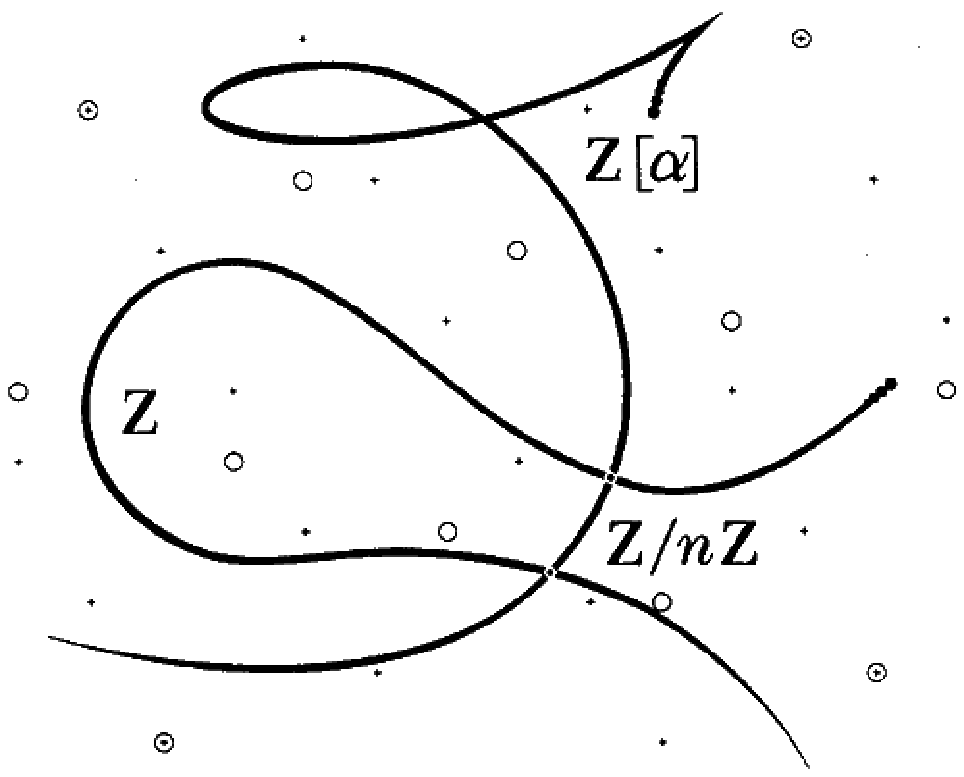
\includegraphics[width=20em]{spec}\\
A diagram from \cite{lenstras:nfs}.
\end{center}

\begin{tabular}{lr}
{\begin{minipage}{4in}
``The obvious mathematical breakthrough would be development of an easy
way to factor large prime numbers.''
\mbox{ }\\\mbox{}\hspace{3em}-- {Bill Gates, {\em The Road Ahead}, 1st ed., pg 265}
\end{minipage}}
&
\begin{minipage}{2in}
\mbox{}\vspace{3ex}

\includegraphics[width=1in]{gates}
\end{minipage}
\\
\end{tabular}

Bill Gates meant\footnote{This quote is on page 265 of the first
  edition.  In the second edition, on page 303, this sentence is
  changed to ``The obvious mathematical breakthrough that would defeat
  our public key encryption would be the development of an easy way to
  factor large numbers.''  This is less nonsensical; however, fast
  factoring is {\em not} known to break all commonly used public-key
  cryptosystem.  For example, there are cryptosystems based on the
  difficulty of computing discrete logarithms in $\F_p^*$ and on
  elliptic curves over $\F_p$, which (presumably) would not be broken
  even if one could factor large numbers quickly.}  factoring products
of two primes, which would break the RSA cryptosystem (see
e.g. \cite[\S 3.2]{stein:ent}).  However, perhaps Gates is an
algebraic number theorist, and he really meant what he said: then we
might imagine that he meant factorization of primes of~$\Z$ in rings
of integers of number fields.  For example, $2^{16}+1 = 65537$ is a
``large'' prime, and in $\Z[i]$ we have
$$ (65537) = (65537, 2^8 + i) \cdot (65537, 2^8 - i).$$

\subsection{Geometric Intuition}
Let $K=\Q(\alpha)$ be a number field, and let $\O_K$ be the ring of
integers of $K$.  To employ our geometric intuition, as the Lenstras
did on the cover of \cite{lenstras:nfs}, it is helpful to
view $\O_K$ as a 1-dimensional scheme
$$
  X = \Spec(\O_K) = \{\text{all prime ideals of $\O_K$}\}
$$
over
$$
  Y=\Spec(\Z) = \{ (0) \} \union \{ p\Z : p \in\Z_{>0} \text{ is prime}\}.
$$
There is a natural map $\pi :X\ra Y$ that sends a prime ideal $\p\in X$ to
$\p\intersect \Z\in Y$.
For example, if
$$
 \p = (65537, 2^8 + i)\subset\Z[i],
$$
then
$\p \intersect \Z = (65537)$.
For more on this viewpoint,
see \cite{hartshorne} and \cite[Ch.~2]{eisenbud_harris:geometry}.

If $p\in\Z$ is a prime number, then the ideal $p\O_K$ of $\O_K$
factors uniquely as a product $\prod \p_i^{e_i}$, where the $\p_i$ are
maximal ideals of $\O_K$.  We may imagine the decomposition of $p\O_K$
into prime ideals geometrically as the fiber $\pi^{-1}(p\Z)$, where
the exponents $e_i$ are the multiplicities of the fibers.  Notice that
the elements of $\pi^{-1}(p\Z)$ are the prime ideals of $\O_K$ that
contain~$p$, i.e., the primes that divide $p\O_K$.
This chapter is about how to compute the $\p_i$ and $e_i$.





\begin{remark}
  More technically, in algebraic geometry one defines the inverse
  image of the point $p\Z$ to be the spectrum of the tensor product
  $\O_K \tensor_{\Z} \Z/\p\Z$; by a generalization of the Chinese
  Remainder Theorem, we have
$$
  \O_K \tensor_{\Z} \left(\Z/\p\Z\right) \isom \oplus \O_K/\p_i^{e_i}.
$$
\end{remark}



\subsection{Examples}
The following \sage session shows the commands needed to compute
the factorization of $p\O_K$ for~$K$ the number field
defined by a root of $x^5+7x^4+3x^2-x+1$ and $p=2$ and~$5$.
We first create an element $f\in \QQ[x]$ in \sage:
\begin{verbatim}
sage: R.<x> = QQ[]
sage: f = x^5 + 7*x^4 + 3*x^2 - x + 1
\end{verbatim}%link

\par\noindent{}Then we create the corresponding number field obtained
by adjoining a root of $f$, and find its ring of integers.
%link
\begin{verbatim}
sage: K.<a> = NumberField(f)
sage: OK = K.ring_of_integers()
sage: OK.basis()
[1, a, a^2, a^3, a^4]
\end{verbatim}%link

\par\noindent{}We define the ideal $2\O_K$ and factor -- it turns
out to be prime.
%link
\begin{verbatim}
sage: I = K.fractional_ideal(2); I
Fractional ideal (2)
sage: I.factor()
Fractional ideal (2)
sage: I.is_prime()
True
\end{verbatim}%link

\par\noindent{}Finally we factor $5\O_K$, which factors as a product of three
primes.
%link
\begin{verbatim}
sage: I = K.fractional_ideal(5); I
Fractional ideal (5)
sage: I.factor()
(Fractional ideal (5, a^2 + 9*a + 2)) * (Fractional ideal (5, a + 2)) \
* (Fractional ideal (5, a + 3))^2
\end{verbatim}
Notice that the polynomial $f$ factors in a similar way:
\begin{verbatim}
sage: f.factor_mod(5)
(x + 2) * (x + 3)^2 * (x^2 + 4*x + 2)
\end{verbatim}
Thus $2\O_K$ is already a prime ideal, and
$$
  5\O_K = (5,2+a)\cdot(5,3+a)^2\cdot(5,2+4a+a^2).
$$
Notice that in this example $\O_K=\Z[a]$.  (Warning: There are
examples of $\O_K$ such that $\O_K\neq \Z[a]$ for any $a\in\O_K$, as
Example~\ref{ex:dedekind} below illustrates.)  When $\O_K=\Z[a]$ it is
relatively easy to factor $p\O_K$, at least assuming one can factor
polynomials in $\F_p[x]$.  The following
factorization gives a hint as to why:
$$
  x^5+7x^4+3x^2-x+1 \con (x+2)\cdot (x+3)^2 \cdot (x^2+4x+2)\pmod{5}.
$$

The exponent~$2$ of $(5,3+a)^2$ in the factorization of $5\O_K$ above
suggests ``ramification'',
in the sense that the cover $X\ra Y$ has less points (counting their ``size'', i.e.,
their residue class degree) in its fiber over~$5$ than
it has generically.

%% \vfill

%% \begin{center}
%% \psfrag{p1}{$(5,2+4a+a^2)$}
%% \psfrag{p2}{$(5,3+a)^2$}
%% \psfrag{p3}{$(5,2+a)$}
%% \psfrag{p}{$5\Z$}
%% \psfrag{q1}{$2\O_K$}
%% \psfrag{q}{$2\Z$}
%% \psfrag{zero}{$(0)$}
%% \psfrag{r}{$3\Z$}
%% \psfrag{s}{$7\Z$}
%% \psfrag{t}{$11\Z$}
%% 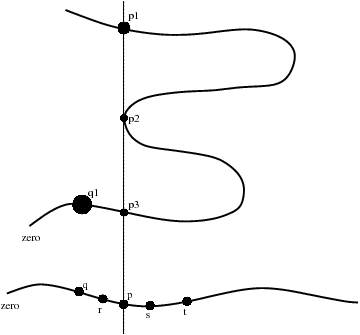
\includegraphics[width=30em]{cover1}\\
%% Diagram of $\Spec(\O_K) \ra \Spec(\Z)$
%% \end{center}


\section{A Method for Factoring Primes that Often Works}
Suppose $a\in\O_K$ is such that $K=\Q(a)$, and let
$f(x)\in\Z[x]$ be the minimal polynomial of~$a$.  Then
$\Z[a]\subset \O_K$, and we have a diagram of schemes
$$\xymatrix{
  {{\ds \bigcup}\Spec(\O_K/\p_i^{e_i})}\ar@{^(->}[r]\ar[d]               &{\Spec(\O_K)}\ar[d]  \\
{{\ds \bigcup}\Spec(\F_p[x]/(\overline{f}_i^{e_i}))\,}\ar@{^(->}[r] \ar[d]
         &{\Spec(\Z[a])}\ar[d] \\%\ar@{=}[r] & \Spec(\Z[x]/f(x))\\
{\Spec(\F_p)\,}\ar@{^(->}[r]&{\Spec(\Z)}
}$$
where $\overline{f} = \prod_i \overline{f}_i^{e_i}$
is the factorization of the image of $f$ in $\F_p[x]$,
and $p\O_K = \prod \p_i^{e_i}$ is the factorization
of $p\O_K$ in terms of prime ideals of $\O_K$.
On the level of rings, the bottom horizontal map
is the quotient map $\Z\to\Z/p\Z\isom \F_p$.
The middle horizontal map is induced by
$$
  \Z[x] \to \bigoplus_i \F_p[x]/(\overline{f}_i^{e_i}),
$$
and the top horizontal map is induced by
$$
  \O_K \to \O_K/p\O_K \isom \bigoplus \O_K/\p_i^{e_i},
$$
where the isomorphism is by the Chinese Remainder Theorem,
which is Theorem~\ref{thm:crt} below.
The left vertical maps come from the inclusions
$$
   \F_p \hra \F_p[x]/(\overline{f}_i^{e_i}) \hra \O_K/\p_i^{e_i},
$$
and the right from the inclusions $\Z\hra\Z[a]\hra\O_K$.

The cover $\pi:\Spec(\Z[a])\ra \Spec(\Z)$ is easy to understand
because it is defined by the single equation $f(x)$, in the sense
that $\Z[a]\isom \Z[x]/(f(x))$.  To give a
maximal ideal~$\p$ of $\Z[a]$ such that $\pi(\p) = p\Z$ is the
same as giving a homomorphism $\vphi:\Z[x]/(f) \ra \Fbar_p$ up to
automorphisms of the image, which is in turn the same as giving a
root of~$f$ in $\Fbar_p$ up to automorphism, which is the same
as giving an irreducible factor of the reduction of~$f$ modulo~$p$.

\begin{lemma}\ilem{factorization of $p\O_K$}\label{lem:factpok}
Suppose the index of $\Z[a]$ in $\O_K$ is coprime to~$p$.  Then
the primes~$\p_i$ in the factorization of $p\Z[a]$ do not
decompose further going from $\Z[a]$ to $\O_K$, so finding the
prime ideals of $\Z[a]$ that contain~$p$ yields the primes
that appear in the factorization of $p\O_K$.
\end{lemma}
\begin{proof}
% {\em Low-brow argument:}
Fix a basis for $\O_K$ and for $\Z[a]$ as $\Z$-modules.
Form the matrix~$A$ whose columns express each basis element
of $\Z[a]$ as a $\Z$-linear combination of the basis for $\O_K$.
Then
$$
\det(A) = \pm [\O_K:\Z[a]]
$$
is coprime to~$p$, by hypothesis.  Thus the reduction of~$A$
modulo~$p$ is invertible, so it defines an isomorphism
$\Z[a]/p\Z[a] \isom \O_K/p\O_K$.

Let $\Fpbar$ denote a fixed algebraic closure of $\F_p$; thus $\Fpbar$
is an algebraically closed field of characteristic~$p$, over which
all polynomials in $\F_p[x]$ factor into linear factors.
Any homomorphism $\O_K\to \Fpbar$ sends~$p$ to~$0$, so is the composition of a homomorphism $\O_K \to \O_K/p\O_K$ with a homomorphism
$\O_K/p\O_K \to \Fpbar$.  Since $\O_K/p\O_K \isom
\Z[a]/p\Z[a]$, the homomorphisms $\O_K\to \Fpbar$ are in bijection
with the homomorphisms $\Z[a]\to \Fpbar$.  The homomorphisms
$\Z[a]\to\Fpbar$ are in bijection with the roots of the reduction
modulo~$p$ of the minimal polynomial of~$a$ in $\Fpbar$.
\end{proof}

\begin{remark}
Here is a ``high-brow'' proof of Lemma~\ref{lem:factpok}.
By hypothesis we have an exact sequence
of abelian groups
$$ 0 \to \Z[a]\to \O_K \to H \to 0,$$
where $H$ is a finite abelian group of order coprime
to~$p$.  Tensor product is right exact, and there is
an exact sequence
$$
   \Tor_1(H,\F_p) \to \Z[a]\tensor\F_p \to \O_K\tensor\F_p \to H\tensor\F_p \to 0,
$$
and $\Tor_1(H,\F_p) = 0$ (since $H$ has no $p$-torsion),
so $\Z[a]\tensor\F_p\isom \O_K\tensor\F_p$.
\end{remark}

As suggested in the proof of the lemma, we find all homomorphisms
$\O_K\to \Fpbar$ by finding all homomorphism $\Z[a]\to \Fpbar$.  In
terms of ideals, if $\p=(f(a),p)\Z[a]$ is a maximal ideal of $\Z[a]$,
then the ideal $\p'=(f(a),p)\O_K$ of $\O_K$ is also maximal, since
$$\O_K/\p'\isom (\O_K/p\O_K)/(f(\tilde{a}))
\isom (\Z[a]/p\Z[a]) / (f(\tilde{a})) \subset \Fpbar,$$
where $\tilde{a}$ denotes the image of $a$ in $\O_K/p\O_K$.

We formalize the above discussion in the following theorem (note: we will
not prove that the powers are $e_i$ here):
\begin{theorem}\label{thm:fac1}\ithm{prime ideal factorization}
Let $f\in\Z[x]$ be the minimal polynomial of~$a$ over~$\Z$.
Suppose that~$p\nmid [\O_K:\Z[a]]$ is a prime.
Let
$$
 \overline{f} = \prod_{i=1}^t \overline{f}_i^{e_i} \in \F_p[x]
$$
where the $\overline{f}_i$ are distinct monic irreducible
polynomials.
Let
$
  \p_i = (p,f_i(a))
$
where $f_i\in\Z[x]$ is a lift of $\overline{f}_i$ in $\F_p[x]$.
Then
$$
  p\O_K = \prod_{i=1}^t \p_i^{e_i}.
$$
%Geometrically, the fiber of $\Spec(\O_K) \to p\Z$
%contains the points $\{\p_1,\p_2,\ldots, \p_t\}$
%with multiplicites $e_i$.
\end{theorem}

We return to the example from above, in which $K=\Q(a)$, where~$a$ is
a root of $f = x^5+7x^4+3x^2-x+1$.  The ring
of integers~$\O_K$ has discriminant $2945785 = 5\cdot 353\cdot 1669$,
as the following \sage code shows.
\begin{verbatim}
sage: K.<a> = NumberField(x^5 + 7*x^4 + 3*x^2 - x + 1)
sage: D = K.discriminant(); D
2945785
sage: factor(D)
5 * 353 * 1669
\end{verbatim}
The order $\Z[a]$ has the same discriminant as $f(x)$, which
is the same as the discriminant of $\O_K$, so
$\Z[a]=\O_K$ and we can apply the above theorem.
(Here we use that the index of $\Z[a]$ in $\O_K$
is the square of the quotient of their discriminants,
a fact we will prove later in Section~\ref{sec:disc}.)
\begin{verbatim}
sage: R.<x> = QQ[]
sage: discriminant(x^5 + 7*x^4 + 3*x^2 - x + 1)
2945785
\end{verbatim}
We have
$$
  x^5+7x^4+3x^2-x+1 \con (x+2)\cdot (x+3)^2 \cdot (x^2+4x+2)\pmod{5},
$$
which yields the factorization of $5\O_K$ given before the theorem.

If we replace $a$ by $b=7a$, then the index of $\Z[b]$
in $\O_K$ will be a power of $7$, which is coprime to $5$,
so the above method will still work.
\begin{verbatim}
sage: K.<a> = NumberField(x^5 + 7*x^4 + 3*x^2 - x + 1)
sage: f = (7*a).minpoly('x')
sage: f
x^5 + 49*x^4 + 1029*x^2 - 2401*x + 16807
sage: f.disc()
235050861175510968365785
sage: factor(f.disc() / K.disc())
7^20
sage: f.factor_mod(5)
(x + 4) * (x + 1)^2 * (x^2 + 3*x + 3)
\end{verbatim}
Thus $5$ factors in $\O_K$
as
$$
  5\O_K = (5, 7a+1)^2 \cdot (5, 7a+4) \cdot (5, (7a)^2 + 3(7a) + 3).
$$
If we replace $a$ by $b=5a$ and try the above algorithm with $\Z[b]$,
then the method fails because the index of $\Z[b]$ in $\O_K$ is divisible
by~$5$.
\begin{verbatim}
sage: K.<a> = NumberField(x^5 + 7*x^4 + 3*x^2 - x + 1)
sage: f = (5*a).minpoly('x')
sage: f
x^5 + 35*x^4 + 375*x^2 - 625*x + 3125
sage: f.factor_mod(5)
x^5
\end{verbatim}

\section{A General Method}
There are numbers fields $K$ such that $\O_K$ is not of the form
$\Z[a]$ for any $a\in K$.  Even worse, Dedekind found a
field~$K$ such that $2\mid [\O_K : \Z[a]]$ for {\em all}
$a\in \O_K$, so there is no choice of $a$ such that
Theorem~\ref{thm:fac1} can be used to factor~$2$ for $K$ (see
Example~\ref{ex:dedekind} below).

\subsection{Inessential Discriminant Divisors}
\begin{definition}
A prime $p$ is an \defn{inessential discriminant
divisor} if $p\mid [\O_K : \Z[a]]$ for
{\em every} $a\in\O_K$.
\end{definition}
See Example~\ref{ex:exdim} below for
why it is called an inessential ``discriminant divisor'' instead
of an inessential ``index divisor''.

Since $[\O_K : \Z[a]]^2$ is the absolute value of
$\Disc(f(x))/\Disc(\O_K)$, where $f(x)$ is the characteristic
polynomial of $f(x)$, an inessential discriminant divisor divides the
discriminant of the characteristic polynomial of any element of
$\O_K$.

\begin{example}[Dedekind]\label{ex:dedekind}
Let $K=\Q(a)$ be the cubic field defined by a root $a$ of the polynomial
$f = x^3 + x^2 - 2x+8$.  We will use \sage to show that~$2$ is an inessential
discriminant divisor for~$K$.
\begin{verbatim}
sage: K.<a> = NumberField(x^3 + x^2 - 2*x + 8); K
Number Field in a with defining polynomial x^3 + x^2 - 2*x + 8
sage: K.factor_integer(2)
(Fractional ideal (1/2*a^2 - 1/2*a + 1)) *
(Fractional ideal (a^2 - 2*a + 3)) *
(Fractional ideal (3/2*a^2 - 5/2*a + 4))
\end{verbatim}
Thus $2\O_K=\p_1\p_2\p_3$, with the $\p_i$ distinct,
and one sees directly from the above expressions
that
$\O_K/\p_i\isom \F_2$ for each $i$.  If $\O_K=\Z[a]$
for some $a\in\O_K$ with minimal polynomial~$f$, then
$\overline{f}(x)\in\F_2[x]$ must be a product of three {\em distinct}
linear factors, which is impossible, since the only
linear polynomials in $\F_2[x]$ are $x$ and $x+1$.
\end{example}

\subsection{Remarks on Ideal Factorization in General}

Recall (from Definition~\ref{defn:order}) that an {\em order} in $\O_K$ is
a subring $\O$ of $\O_K$ that has finite index in $\O_K$.  For
example, if $\O_K=\Z[i]$, then $\O=\Z + 5\Z[i]$ is an order in $\O_K$,
and as an abelian group $\O_K/\O$ is cyclic of order~$5$.

Most algebraic number theory books do not describe an algorithm for
decomposing primes in the general case.  Fortunately, Cohen's book
\cite[Ch.~6]{cohen:course_ant} does describe how to solve the general
problem, in more than one way.  The algorithms are nontrivial, and
occupy a substantial part of Chapter~6 of Cohen's book.  Our goal
for the rest of this section is to give a hint as to what goes into them.

The general solutions to prime ideal factorization are somewhat surprising,
since the algorithms are much more sophisticated than the one
suggested by Theorem~\ref{thm:fac1}.  However, these complicated
algorithms all run very quickly in practice, even without assuming the
maximal order is already known.  In fact, they avoid computing~$\O_K$
altogether, and instead compute only an order~$\O$ that is {\em
  $p$-maximal}, i.e., is such that $p \nmid [\O_K:\O]$.

For simplicity we consider the following slightly easier problem whose
solution illustrates the key ideas needed in the general case.
\begin{problem}\label{prob:pcontained}
Let $\O$ be any order in $\O_K$
and let~$p$ be a prime of $\Z$.  Find the prime ideals of $\O$ that
contain~$p$.
\end{problem}

Given a prime~$p$
that we wish to factor in $\O_K$, we first find a $p$-maximal order~$\O$.
We then use a solution to Problem~\ref{prob:pcontained} to find
the prime ideals $\p$ of $\O$ that contain $p$.  Second, we find
the exponents $e$ such that $\p^e$ exactly divides $p\O$.
The resulting factorization in $\O$ completely determines
the factorization of $p\O_K$.

A $p$-maximal order can be found reasonably quickly in practice using
algorithms called ``round 2'' and ``round 4''.  To
compute $\O_K$, given an order $\Z[\alpha]\subset \O_K$, one takes a
sum of $p$-maximal orders, one for every~$p$ such that $p^2$ divides
$\Disc(\Z[\alpha])$.  The time-consuming part of this computation is
finding the primes~$p$ such that $p^2\mid \Disc(\Z[\alpha])$, not
finding the $p$-maximal orders.  This example illustrates that
a fast algorithm for factoring integers would not only break the RSA
cryptosystems, but would massively speed up computation of the ring of
integers of a number field.
\begin{remark}
The MathSciNet review of \cite{buchmann_lenstra:approx} by
J.~Buhler contains the following:
\begin{quote}
    A result of Chistov says that finding the ring of integers $\O_K$
    in an algebraic number field $K$ is equivalent, under certain
    polynomial time reductions, to the problem of finding the largest
    squarefree divisor of a positive integer. No feasible (i.e.,
    polynomial time) algorithm is known for the latter problem, and it
    is possible that it is no easier than the more general problem of
    factoring integers.
\end{quote}
Thus it appears that computing the ring $\O_K$ is quite hard.
\end{remark}

\subsection{Finding a $p$-Maximal Order}\label{sec:alg_pmax}
Before describing the general factorization algorithm, we sketch some
of the theory behind the general algorithms for computing a
$p$-maximal order $\O$ in $\O_K$.  The main input is the following
theorem:
\begin{theorem}[Pohst-Zassenhaus]
Let $\O$ be an order in the the ring of integers $\O_K$ of a number field, let $p\in\Z$ be a prime,
and let
$$I_p = \{x \in \O : x^m \in p\O \text{ for some $m\geq 1$}\} \subset \O$$
be the radical of $p\O$, which is an ideal of $\O$.
Let
$$
  \O' = \{x \in K : xI_p \subset I_p\}.
$$
Then $\O'$ is an order and either $\O'=\O$, in which case $\O$ is
$p$-maximal, or $\O\subset\O'$ and $p$ divides $[\O':\O]$.
\end{theorem}
\begin{proof}
  We prove here only that $[\O':\O] \mid p^n$, where $n$ is the degree
  of $K$.  We have $p\in I_p$, so if $x \in \O'$, then $xp \in
  I_p\subset \O$, which implies that $x\in \frac{1}{p}\O$.  Since
  $(\frac{1}{p}\O)/\O$ is of order $p^n$, the claim follows.

To complete the proof, we would show that if $\O' = \O$, then $\O$ is
already $p$-maximal.  See \cite[\S6.1.1]{cohen:course_ant} for the
rest if this proof.
\end{proof}

After deciding on how to represent elements of~$K$ and orders and
ideals in~$K$, one can give an efficient algorithm to compute the
$\O'$ of the theorem.  The algorithm mainly involves linear algebra
over finite fields.  It is complicated to describe, but efficient in
practice, and is conceptually simple---just compute~$\O'$.  The trick
for reducing the computation of $\O'$ to linear algebra is the
following lemma:
\begin{lemma}
  Define a homomorphism $\psi:\O \hra \End(I_p/ p I_p)$ given by
  sending $\alpha\in\O$ to left multiplication by the reduction of
  $\alpha$ modulo~$p$.  Then
$$
   \O'=\frac{1}{p} \Ker(\psi).
$$
\end{lemma}
\begin{proof}
If $x \in \O'$, then $x I_p \subset I_P$, so $\psi(x)$ is the $0$
endomorphism.  Conversely, if $\psi(x)$ acts as $0$ on $I_p/ p I_p$,
then clearly $x I_p \subset I_p$.
\end{proof}

Note that to give an algorithm one must also figure out how to
explicitly compute $I_p/ p I_p$ and the kernel of this map
(see  the next section for more
details).


\subsection{General Factorization Algorithm of Buchman-Lenstra}
We finally give an algorithm to factor $p\O_K$ in general. This is a
summary of the algorithm described in more detail in
\cite[\S6.2]{cohen:course_ant}.

\begin{algorithm}[Factoring a Finite Separable Algebra]\label{alg:factorsep}
Let $A$ be a finite separable algebra over $\F_p$.  This
algorithm either shows that $A$ is a field or finds
a nontrivial idempotent in $A$, i.e., an $\eps\in A$
such that $\eps^2 = \eps$ with $\eps\neq 0$ and $\eps\neq 1$.
\begin{enumerate}
\item The dimension of the kernel $V$ of the map $x\mapsto x^p - x$ is
  equal to $k$.  This is because abstractly we have that $A\ncisom
  A_1\times \cdots \times A_k$, with each $A_i$ a finite field
  extension of $\F_p$.
\item If $k=1$ we are done.  Terminate.
\item Otherwise, choose $\alpha \in V$ with $\alpha \not\in \F_p$.
(Think of $\F_p$ as the diagonal embedding of $\F_p$ in
$A_1\times \cdots \times A_k$).
Compute powers of $\alpha$ and find the minimal polynomial $m(X)$
of $\alpha$.
\item Since $V\ncisom \F_p \times \cdots \times F_p$ ($k$ factors),
the polynomial $m(X)$ is a square-free product of linear factors, that
has degree $>1$ since $\alpha\not\in\F_p$.  Thus we can compute
a splitting $m(X) = m_1(X) \cdot m_2(X)$, where both $m_i(X)$ have
positive degree.
\item Use the Euclidean algorithm in $\F_p[X]$ to find
$U_1(X)$ and $U_2(X)$ such that
$$
  U_1 m_1 + U_2 m_2 = 1.
$$
\item Let $\eps = (U_1 m_1)(\alpha)$.  Then we have
$$
  U_1 m_1 U_1 m_1 + U_2 m_2 U_1 m_1 = U_1 m_1,
$$
so since $(m_1 m_2)(\alpha) = m(\alpha)=01$, we have $\eps^2 = \eps$.
Also, since $\gcd(U_1, m_2) = \gcd(U_2, m_1) = 1$,
we have $\eps\neq 0$ and $\eps \neq 1$.
\end{enumerate}
\end{algorithm}

Given Algorithm~\ref{alg:factorsep}, we compute an idempotent
$\eps \in A$, and observe that
$$
 A \isom \Ker(1 - \eps)  \oplus \Ker(\eps).
$$
Since $(1 - \eps) + \eps = 1$, we see that
$(1 - \eps)v + \eps v = v$, so that the sum
of the two kernels equals $A$.
Also, if $v$ is in the intersection of the two kernels,
then $\eps(v) = 0$ and $(1-\eps)(v) =0$, so
$0 = (1-\eps)(v) = v - \eps(v) = v$, so the sum is direct.

\begin{remark}
  The beginning of \cite[\S6.2.4]{cohen:course_ant} suggests that one
  can just randomly find an $\alpha \in A$ such that $A\isom
  \F_p[x]/(m(x))$ where $m$ is the minimal polynomial of $\alpha$.
  This is usually the case, but is {\em wrong in general}, since there
  need {\em not} be an $\alpha \in A$ such that $A \isom
  \F_p[\alpha]$.  For example, let $p=2$ and $K$ be as in
  Example~\ref{ex:dedekind}.  Then $A\isom \F_2 \times \F_2 \times
  \F_2$, which as a ring is not generated by a single element, since
  there are only 2 distinct linear polynomials over $\F_2[x]$.
\end{remark}

\begin{algorithm}[Factoring a General Prime Ideal]\label{alg:genfac}
Let $K=\Q(a)$ be a number field given
by an algebraic integer~$a$ as a root of its
minimal monic polynomial~$f$ of degree~$n$.
We assume that an order $\O$ has been
given by a basis $w_1,\ldots,w_n$
and that~$\O$ that contains $\Z[a]$.
For any prime $p\in\Z$, the following
algorithm computes the set of maximal ideals of~$\O$ that contain~$p$.
\begin{enumerate}
\item{} [Check if easy] If $p\nmid \disc(\Z[a]) / \disc(\O)$ (so
$p\nmid [\O:\Z[a]]$), then using Theorem~\ref{thm:fac1} we
factor~$p\O$.
\item{} [Compute radical]
Let $I$ be the \defn{radical} of $p\O$, which is the ideal of
elements $x\in\O$ such that $x^m\in p\O$
for some positive integer~$m$.  Note that $p\O \subset I$, i.e.,
$I\mid p\O$; also~$I$ is the product
of the primes that divide $p$, without multiplicity.
Using linear algebra over the finite field
$\F_p$, we compute a basis for $I/p\O$ by computing
the abelian subgroup of $\O/p\O$ of all nilpotent
elements.  This computes $I$, since $p\O\subset I$.
\item{} [Compute quotient by radical]
Compute an $\F_p$ basis for
$$
  A = \O/I = (\O/p\O)/(I/p\O).
$$
The second equality comes from the fact that $p\O\subset I$.
Note that $\O/p\O$
is obtained by simply reducing the basis $w_1,\ldots, w_n$ modulo~$p$.
Thus this step entirely involves linear algebra modulo $p$.

\item{} [Decompose quotient] The ring $A$ is isomorphic to
the quotient of $\O$ by a radical ideal,
so it decomposes as a product
$A \isom A_1 \times \cdots \times A_k$ of finite fields.
We find such a decomposition explicitly using Algorithm~\ref{alg:factorsep}.

\item{} [Compute the maximal ideals over $p$] Each maximal ideal
  $\p_i$ lying over~$p$ is the kernel of one of the compositions
$$\O \to A \ncisom A_1 \times \cdots \times A_k \to A_i.$$
\end{enumerate}
\end{algorithm}
Algorithm~\ref{alg:genfac} finds all primes of $\O$ that contain the radical $I$ of
$p\O$.  Every such prime clearly contains $p$, so to see that the
algorithm is correct, we prove that the primes $\p$ of $\O$ that
contain~$p$ also contain~$I$.  If $\p$ is a prime of $\O$ that
contains~$p$, then $p\O \subset \p$.  If $x\in I$ then $x^m\in p\O$
for some $m$, so $x^m\in \p$ which implies that $x\in \p$ by the primality
of $\p$.  Thus $\p$ contains $I$, as required.  Note that we do not find the powers of
primes that divide $p$ in Algorithm~\ref{alg:genfac}; that's left to another
algorithm that we will not discuss in this book.

Algorithm~\ref{alg:genfac} was invented by J.~Buchmann and
H.\thinspace{}W. Lenstra, though their paper seems to have never been
published; however, the algorithm is described in detail in
\cite[\S6.2.5]{cohen:course_ant}.  Incidentally, this chapter is based
on Chapters~4 and~6 of \cite{cohen:course_ant}, which is highly
recommended, and goes into much more detail about these algorithms.


%%[[Add discussion about how to compute a $p$-maximal order here.]]


%\section{Appendix: The Calculations in PARI}\label{sec:factor_pari}
%In this section we give PARI versions of all the \magma{} calculations
%in the rest of this chapter.
%\begin{verbatim}
%   ? K = nfinit(x^5 + 7*x^4 + 3*x^2 - x + 1);
%   ? idealfactor(K, 2)
%   [[2, [2, 0, 0, 0, 0]~, 1, 5, [1, 0, 0, 0, 0]~] 1]
%   ? idealfactor(K, 5)
%   [[5, [-3, 0, 0, 1, 0]~, 2, 1, [1, 0, 2, -2, -1]~] 2]
%   [[5, [1, 0, 0, 1, 0]~, 1, 1, [1, 0, -2, 2, -1]~] 1]
%   [[5, [10, 1, 0, -8, 1]~, 1, 2, [2, 1, 1, -1, 1]~] 1]
%
%   ? K.disc
%   2945785
%
%   ? poldisc(x^5 + 7*x^4 + 3*x^2 - x + 1)
%   2945785
%
%   ? a = Mod(x, x^5 + 7*x^4 + 3*x^2 - x + 1);
%   ? f = charpoly(7*a)
%   x^5 + 49*x^4 + 1029*x^2 - 2401*x + 16807
%   ? poldisc(f)
%   235050861175510968365785
%   ? poldisc(f)/K.disc
%   79792266297612001
%   ? factormod(f,5)
%   [Mod(1, 5)*x + Mod(1, 5) 2]
%   [Mod(1, 5)*x + Mod(4, 5) 1]
%   [Mod(1, 5)*x^2 + Mod(3, 5)*x + Mod(3, 5) 1]
%
%   ? f = charpoly(5*a)
%   ? factormod(f,5)
%   [Mod(1, 5)*x 5]
%
%   ? K = nfinit(x^3 + x^2 - 2*x + 8);
%   ? idealfactor(K,2)
%   [[2, [1, 0, 1]~, 1, 1, [0, 0, -1]~] 1]
%   [[2, [1, 1, 0]~, 1, 1, [0, 1, 0]~] 1]
%   [[2, [2, 1, 1]~, 1, 1, [1, 1, 1]~] 1]
%\end{verbatim}
%



%%% Local Variables:
%%% mode: latex
%%% TeX-master: "ant"
%%% End:

\chapter{The Chinese Remainder Theorem}\label{ch:crt}
In this chapter, we prove the Chinese Remainder Theorem (CRT) for
arbitrary commutative rings, then apply CRT to prove that every ideal
in a Dedekind domain $R$ is generated by at most two elements.  We
also prove that $\p^n/\p^{n+1}$ is (noncanonically) isomorphic to
$R/\p$ as an $R$-module, for any nonzero prime ideal $\p$ of $R$.  The
tools we develop in this chapter will be used frequently to prove
other results later.

\section{The Chinese Remainder Theorem}

\subsection{CRT in the Integers}
The classical CRT asserts that if $n_1,\ldots, n_r$ are integers that are coprime
in pairs, and $a_1,\ldots, a_r$ are integers, then there exists an
integer~$a$ such that $a\con a_i\pmod{n_i}$ for each $i=1,\ldots,r$.
Here ``coprime in pairs'' means that $\gcd(n_i,n_j)=1$ whenever
$i\neq j$; it does {\em not} mean that $\gcd(n_1,\ldots, n_r)=1$,
though it implies this. 
In terms of rings, CRT asserts that the
natural map
\begin{equation}\label{eqn:crt}
\Z/(n_1\cdots n_r)\Z \to (\Z/n_1\Z)\oplus \cdots \oplus (\Z/n_r\Z)
\end{equation}
that sends $a \in \Z$ to its reduction modulo each $n_i$,
is an isomorphism.  

This map is {\em never} an isomorphism if the $n_i$ are not coprime.
Indeed, the cardinality of the image of the left hand side of
(\ref{eqn:crt}) is $\lcm(n_1,\ldots, n_r)$, since it is the image of a
cyclic group and $\lcm(n_1,\ldots, n_r)$ is the largest order of an
element of the right hand side, whereas the cardinality of the right
hand side is $n_1\cdots n_r$.

The isomorphism (\ref{eqn:crt}) can alternatively be viewed as
asserting that any system of linear congruences
$$
  x \con a_1 \pmod{n_1}, \quad  
x \con a_2 \pmod{n_2}, \quad
\ldots, \quad
x \con a_r \pmod{n_r}
$$
with pairwise coprime moduli has a unique solution modulo $n_1\cdots n_r$.

Before proving the CRT in more generality, we prove
(\ref{eqn:crt}).
There is a natural map 
$$
  \phi: \Z \to (\Z/n_1\Z)\oplus \cdots \oplus (\Z/n_r\Z)
$$
given by projection onto each factor.  Its kernel is
$$
 n_1 \Z \cap \cdots \cap n_r \Z.
$$ 
If $n$ and $m$ are integers, then $n\Z\cap m\Z$ is the
set of multiples of both $n$ and $m$, so $n\Z\cap m\Z = \lcm(n,m)\Z$.
Since the $n_i$ are coprime, 
$$
 n_1 \Z \cap \cdots \cap n_r \Z = n_1 \cdots n_r \Z.
$$ 
Thus we have proved there is an inclusion 
\begin{equation}\label{eqn:crt_inj}
 i: \Z/(n_1\cdots n_r)\Z \hra (\Z/n_1\Z)\oplus \cdots \oplus (\Z/n_r\Z).
\end{equation}
This is half of the CRT; the other half is to prove that this map is
surjective.  In this case, it is clear that $i$ is also surjective,
because $i$ is an injective map between finite sets of the same cardinality.
We will, however, give a proof of surjectivity that doesn't use
finiteness of the above two sets.

To prove surjectivity of $i$, note that since the $n_i$ are coprime in
pairs, $$\gcd(n_1, n_2\cdots n_r)=1,$$ so there exists integers $x,y$
such that
$$
   x n_1 + y n_2\cdots n_r = 1.
$$
To complete the proof, observe that 
$ y n_2\cdots n_r = 1 - x n_1$
is congruent to~$1$ modulo $n_1$ and~$0$ modulo $n_2\cdots n_r$.
Thus $(1,0,\ldots,0) = i (y n_2\cdots n_r)$ is in the image of~$i$.  
By a similar argument, we see that $(0,1,\ldots,0)$ and the
other similar elements are all in the image of~$i$, so $i$
is surjective, which proves CRT.  

\subsection{CRT in General}
Recall that {\em all rings in this book are commutative with unity}.
Let $R$ be such a ring.
\begin{definition}[Coprime]
Ideals $I$ and $J$ of $R$ are \defn{coprime} if $I+J=(1)$.
\end{definition}
For example, if~$I$ and~$J$ are nonzero ideals in a Dedekind domain,
then they are coprime precisely when the prime ideals that appear in
their two (unique) factorizations are disjoint.

\begin{lemma}\label{lem:prodint}\ilem{$I\cap{}J = IJ$}
If $I$ and $J$ are coprime ideals in a ring $R$, then
$I\cap{}J = IJ$.
\end{lemma}
\begin{proof}
Choose $x\in I$ and $y\in J$
such that $x+y=1$.  If $c\in{} I\cap{} J$ then 
$$c=c\cdot 1=c\cdot (x+y) = cx + cy \in IJ + IJ = IJ,$$
so $I\cap{} J\subset IJ$.  
The other inclusion is obvious by the definition of an ideal.
\end{proof}

\begin{lemma}\label{lem:coprime_prod}
Suppose $I_1,\ldots, I_s$ are pairwise coprime ideals.
Then $I_1$ is coprime to the product $I_2\cdots I_s$.
\end{lemma}
\begin{proof}
In the special case of a Dedekind domain, we could easily
prove this lemma using unique factorization of ideals as
products of primes (Theorem~\ref{thm:intuniqfac}); instead,
we give a direct general argument.

It suffices to prove the lemma in the case $s=3$, since the
general case then follows from induction.
By assumption, there
are $x_1 \in I_1, y_2 \in I_2$ and $a_1 \in I_1, b_3 \in I_3$
such
$$ 
x_1 + y_2 = 1 \qquad\text{and}\qquad a_1 + b_3 = 1.
$$
Multiplying these two relations yields
$$
x_1 a_1 + x_1 b_3 + y_2 a_1 + y_2 b_3 = 1 \cdot 1 = 1.
$$
The first three terms are in $I_1$ and the last term is in 
$I_2 I_3 = I_2 \cap I_3$ (by Lemma~\ref{lem:prodint}), 
so $I_1$ is coprime to $I_2 I_3$.
\end{proof}

Next we prove the general Chinese Remainder Theorem.
We will apply this result with $R=\O_K$ in the rest of this chapter.
\begin{theorem}[Chinese Remainder Theorem]\label{thm:crt}
\ithm{chinese remainder}
Suppose $I_1,\ldots, I_r$ are nonzero ideals of a ring~$R$ such 
$I_m$ and $I_n$ are coprime for any $m\neq n$.  Then the natural
homomorphism $R \to \bigoplus_{n=1}^r R/I_n$ induces an isomorphism
$$
\psi: R/\prod_{n=1}^r I_n \to \bigoplus_{n=1}^r R/I_n.
$$
Thus given any $a_n \in R$, for $n=1,\ldots,r$, there exists some $a\in R$
such that $a\con a_n\pmod{I_n}$ for $n=1,\ldots, r$; moreover,~$a$ 
is unique modulo $\prod_{n=1}^r I_n$.
\end{theorem}

\begin{proof}
Let 
$
  \vphi:R \to \bigoplus_{n=1}^r R/I_n
$
be the natural map induced by reduction modulo
the $I_n$.  
An inductive application of Lemma~\ref{lem:prodint} 
implies that
the kernel $\cap_{n=1}^r I_n$ of~$\vphi$ 
is equal to 
$\prod_{n=1}^r I_n$, so the map~$\psi$ of the theorem is injective.  

Each projection $R\to R/I_n$ is  surjective, so to prove
that $\psi$ is surjective, it suffices 
to show that $(1,0,\ldots,0)$
is in the image of~$\vphi$, and similarly for the other
factors.  By Lemma~\ref{lem:coprime_prod}, 
$J=\prod_{n=2}^rI_n$ is coprime to~$I_1$, so
there exists $x\in I_1$ and $y \in J$ such that
$x+y=1$.  Then $y = 1-x$ maps to~$1$ in 
$R/I_1$ and to~$0$ in $R/J$, hence to~$0$ in $R/I_n$
for each $n\geq 2$, since $J\subset I_n$. 
\end{proof}

\section{Structural Applications of the CRT}
Let $\O_K$ be the ring of integers of some number field $K$, and
suppose~$I$ is a nonzero ideal of $\O_K$.  As an abelian group $\O_K$
is free of rank $[K:\Q]$, and~$I$ is of finite index in $\O_K$, so~$I$
is generated by $[K:\Q]$ generators as an abelian group, so as an
$R$-ideal $I$ requires at most $[K:\Q]$ generators.  The main result
of this section asserts something better, namely that~$I$ can be
generated {\em as an ideal} by at most two elements.  Moreover, our
result is more general, since it applies to an arbitrary Dedekind
domain $R$. Thus, for the rest of this section, $R$ is any Dedekind
domain, e.g., the ring of integers of either a number field or
function field.  We use CRT to prove that every ideal of $R$ can be
generated by two elements.  

\begin{remark}
Caution -- If we replace $R$ by an order in a Dedekind domain, i.e.,
by a subring of finite index,then there may be ideals that require far more than $2$ generators. 
\end{remark}

Suppose that~$I$ is a nonzero integral ideal of
$R$.  If $a\in I$, then $(a)\subset I$, so~$I$ divides~$(a)$ and
the quotient $(a)I^{-1}$ is an integral ideal.  The following lemma
asserts that~$(a)$ can be chosen so the quotient $(a)I^{-1}$ is coprime to
any given ideal.
\begin{lemma}\label{lem:magica}
If $I$ and $J$ are nonzero integral ideals in $R$, then there exists
an $a\in I$ such that the integral ideal $(a)I^{-1}$ is coprime to~$J$.
\end{lemma}
Before we give the proof in general, note that the lemma is trivial
when $I$ is principal, since if $I=(b)$, just take $a=b$, and 
then $(a)I^{-1} = (a)(a^{-1})= (1)$ is coprime to every ideal.
\begin{proof}
Let $\p_1,\ldots, \p_r$ be the prime divisors of~$J$.
For each $n$, let $v_n$ be the largest power of $\p_n$
that divides~$I$.  
Since $\p_n^{v_n}\neq \p_n^{v_n+1}$, 
we can choose an element $a_n\in \p_n^{v_n}$
that is not in $\p_n^{v_n+1}$.
By Theorem~\ref{thm:crt} applied to
the $r+1$ coprime integral ideals
$$
  \p_1^{v_1+1}, \ldots, \p_r^{v_r+1}, \, I\cdot \left(\prod \p_n^{v_n}\right)^{-1},
$$
there exists $a\in R$
such that
$$
   a \con a_n \pmod{\p_n^{v_n+1}}
$$
for all $n=1,\ldots, r$ and
also 
$$
   a \con 0 \quad \left(\text{mod}\,\,\, I\cdot \left(\prod \p_n^{v_n}\right)^{-1}\right).
$$

To complete the proof we show that $(a)I^{-1}$ is not
divisible by any $\p_n$, or equivalently, that each 
$\p_n^{v_n}$ exactly divides $(a)$. 
First we show that $\p_n^{v_n}$ divides $(a)$. Because
$a\con a_n \pmod{\p_n^{v_n+1}}$, there exists 
$b \in \p_n^{v_n+1}$ such that $a = a_n + b$.  Since
$a_n\in \p_n^{v_n}$ and $b \in \p_n^{v_n + 1} \subset \p_n^{v_n}$, 
it follows that $a\in \p_n^{v_n}$,
so $\p_n^{v_n}$ divides~$(a)$.  
Now assume for the sake of contradiction that
$\p_n^{v_n+1}$ divides $(a$); then $a_n=a-b\in \p_n^{v_n+1}$, which
contradicts that we chose $a_n \not\in\p_n^{v_n+1}$.
Thus
$\p_n^{v_n+1}$ does not divide $(a)$, as claimed. 
\end{proof}



\begin{proposition}\iprop{ideals generated by two elements}\label{prop:2gen}
Suppose $I$ is a fractional ideal in a Dedekind domain $R$.  Then there exist $a,b\in{}K$ such that 
$I=(a,b)=\{\alpha a + \beta b : \alpha,\beta \in R\}$.
\end{proposition}
\begin{proof}
If $I=(0)$, then $I$ is generated by $1$ element and we are done.  If
$I$ is not an integral ideal, then there is an $x\in K$ such that $xI$ is
an integral ideal, and the number of generators of $xI$ is the same as
the number of generators of $I$, so we may assume that $I$ is an
integral ideal.  

Let $a$ be {\em any} nonzero element of the integral ideal~$I$.  We
will show that there is some $b\in I$ such that $I=(a,b)$.  Let
$J=(a)$.  By Lemma~\ref{lem:magica}, there exists $b\in I$ such that
$(b)I^{-1}$ is coprime to $(a)$.  Since $a,b\in I$, we have $I\mid
(a)$ and $I\mid (b)$, so $I\mid (a,b)$.  Suppose $\p^n\mid (a,b)$ with
$\p$ prime and $n\geq 1$.  Then $\p^n\mid (a)$ and $\p^n\mid (b)$, so
$\p\nmid (b)I^{-1}$, since $(b)I^{-1}$ is coprime to $(a)$.  We have
$\p^n\mid(b) = I\cdot (b)I^{-1}$ and $\p\nmid (b)I^{-1}$, so $\p^n
\mid I$.  Thus by unique factorization of ideals in $R$ we
have that $(a,b)\mid I$.  Since $I \mid (a,b)$ we conclude
that  $I=(a,b)$, as claimed.
\end{proof}

We can also use Theorem~\ref{thm:crt} to determine the
$R$-module structure of $\p^n/\p^{n+1}$.
\begin{proposition}\label{prop:quopow}\iprop{structure of $\p^n/\p^{n+1}$}
Let $\p$ be a nonzero prime ideal of $R$, and let $n\geq 0$ be an
integer.  Then $\p^n/\p^{n+1} \isom R/\p$ as $R$-modules.
\end{proposition}
\begin{proof}[Proof~\footnote{Proof from \cite[pg.~13]{sd:brief}.}]
Since $\p^n\neq \p^{n+1}$, by unique factorization, 
there is an element $b\in
\p^n$ such that $b\not\in \p^{n+1}$.  Let
$\vphi:R\to\p^n/\p^{n+1}$ be the $R$-module morphism defined by
$\vphi(a)=ab$.  The kernel of $\vphi$ is $\p$ since clearly
$\vphi(\p)=0$ and if $\vphi(a)=0$ then $ab\in\p^{n+1}$, so
$\p^{n+1}\mid (a)(b)$, so $\p\mid (a)$, since $\p^{n+1}$ does not
divide~$(b)$.  Thus~$\vphi$ induces an injective $R$-module
homomorphism $R/\p\hra \p^{n}/\p^{n+1}$.

It remains to show that $\vphi$ is surjective, and this is where we
will use Theorem~\ref{thm:crt}.   Suppose $c\in \p^{n}$.
By Theorem~\ref{thm:crt} there exists $d\in R$
such that
$$
  d \con c\pmod{\p^{n+1}}
\qquad\text{and}\qquad
  d \con 0\pmod{(b)/\p^{n}}.
$$
We have $\p^n\mid (d)$ since $d\in\p^n$ and $(b)/\p^n\mid (d)$
by the second displayed condition, so 
since $\p\nmid(b)/\p^n$, we have $(b)=\p^n\cdot(b)/\p^n\mid (d)$, hence 
$d/b\in R$.   Finally
\[
 \vphi\left(\frac{d}{b}\right) \quad \equiv \quad \frac{d}{b}\cdot b \pmod{\p^{n+1}} 
 \quad \equiv \quad d\pmod{\p^{n+1}} \quad\equiv \quad c\pmod{\p^{n+1}},
\]
so $\vphi$ is surjective.
\end{proof}

\begin{exercise}\label{ex:residuefieldofpower}(See \cite[Theorem~22(a)]{marcus1977number}) %pg 67
	Let $R$ be a Dedekind domain and $\p$ a nonzero prime ideal in $R$.
	Show that $\#(R/\p^m) = \#(R/\p)^m$.
	
	Note: $\#(R/\p)$ is not finite in general! For example,
	The ring of formal power series $k[[t]]$ for some field $k$
	is a Dedekind domain and the residue field at the prime $(t)$
	is $k$.
	
	Hint: Consider the exact sequence
	$$
	0\to \p/\p^{m} \to R/\p^{m} \to R/\p^{m-1} \to 0.
	$$
%%%More hint%%%
%	and the chain
%	$$
%	\p^m \subseteq \p^{m-1} \subseteq \cdots \subseteq \p^2 \subseteq \p
%	$$
\end{exercise}

\begin{remark}
	There is one special case of the previous exercise that you probably
	have seen before: the size of $\Z/4\Z$ is the same as
	$(\Z/2\Z)^2$. In fact you might have seen a proof of
	the fact that $\Z/n^m\Z$ has the same cardinality as $\left(\Z/n\Z\right)^m$
	in a standard group theory or abstract algebra course.
\end{remark}

\section{Computing Using the CRT}
In order to explicitly compute an $a$ as given by Theorem~\ref{thm:crt},
usually one first precomputes elements $v_1, \ldots, v_r \in R$ such that
$v_1\mapsto (1,0,\ldots, 0)$, 
$v_2\mapsto (0,1,\ldots, 0)$, etc.
Then given any $a_n \in R$, for $n=1,\ldots, r$, we obtain an $a \in R$
with $a_n\con a\pmod{I_n}$ by taking
$$
  a = a_1 v_1 + \cdots + a_r v_r.
$$
How to compute the $v_i$ depends on the ring~$R$.   It reduces to
the following problem: Given coprimes ideals $I,J\subset R$, find
$x\in I$ and $y\in J$ such that $x+y=1$.   If $R$ is torsion free and
of finite rank 
as a $\Z$-module, so $R\ncisom \Z^n$,
then $I, J$ can be represented by giving a basis in terms of a basis
for~$R$, and finding $x,y$ such  that $x+y=1$ can then be reduced to 
a problem in linear algebra over~$\Z$.  
More precisely, let~$A$
be the matrix whose columns are the concatenation of a basis for~$I$
with a basis for~$J$.  
Suppose $v\in \Z^n$ corresponds to $1\in\Z^n$.
Then finding $x,y$ such that $x+y=1$ is equivalent to
finding a solution $z\in \Z^n$ to the matrix equation
$Az = v$. This latter linear algebra problem
can be solved using Hermite normal form 
(see \cite[\S4.7.1]{cohen:course_ant}),
which is a generalization over $\ZZ$
of reduced row echelon form.

%We next describe how to use \magma{} and PARI to do CRT computations.

\subsection{\SAGE{}}
[[TODO]]

\subsection{\magma{}}
The \magma{} command {\tt ChineseRemainderTheorem} implements the
algorithm suggested by Theorem~\ref{thm:crt}.  In the following example,
we compute a prime over~$(3)$ and a prime over~$(5)$ of the ring of
integers of $\Q(\sqrt[3]{2})$, and find an element of $\O_K$ that is
congruent to $\sqrt[3]{2}$ modulo one prime and~$1$ modulo the other.
\begin{verbatim}
   > R<x> := PolynomialRing(RationalField());
   > K<a> := NumberField(x^3-2);
   > OK := RingOfIntegers(K);
   > I := Factorization(3*OK)[1][1];
   > J := Factorization(5*OK)[1][1];
   > I;
   Prime Ideal of OK
   Two element generators:
       [3, 0, 0]
       [4, 1, 0]
   > J;
   Prime Ideal of OK
   Two element generators:
       [5, 0, 0]
       [7, 1, 0]
   > b := ChineseRemainderTheorem(I, J, OK!a, OK!1);
   > K!b;
   -4
   > b - a in I;
   true
   > b - 1 in J;
   true
\end{verbatim}

\subsection{PARI}
There is also a CRT algorithm for number fields in PARI, but it
is more cumbersome to use.  First we defined $\Q(\sqrt[3]{2})$
and factor the ideals $(3)$ and $(5)$.
\begin{verbatim}
   ? f = x^3 - 2;
   ? k = nfinit(f);
   ? i = idealfactor(k,3);
   ? j = idealfactor(k,5);
\end{verbatim}

Next we form matrix whose rows correspond to a product of two primes,
one dividing $3$ and one dividing $5$:
\begin{verbatim}
   ? m = matrix(2,2);       
   ? m[1,] = i[1,];  
   ? m[1,2] = 1;
   ? m[2,] = j[1,];
\end{verbatim}
Note that we set {\tt m[1,2] = 1}, so the exponent is 1
instead of $3$.
We apply the CRT to obtain a lift in terms
of the basis for $\O_K$. 
\begin{verbatim}
   ? ?idealchinese
   idealchinese(nf,x,y): x being a prime ideal factorization and y 
   a vector of elements, gives an element b such that 
   v_p(b-y_p)>=v_p(x) for all prime ideals p dividing x, 
   and v_p(b)>=0 for all other p.
   ? idealchinese(k, m, [x,1])
   [0, 0, -1]~
   ? nfbasis(f)
   [1, x, x^2]
\end{verbatim}
Thus PARI finds the lift $-(\sqrt[3]{2})^2$, and we finish by
verifying that this lift is correct.  I couldn't figure out how to
test for ideal membership in PARI, so here we just check that the
prime ideal plus the element is not the unit ideal, which since the
ideal is prime, implies membership.
\begin{verbatim}
   ? idealadd(k, i[1,1], -x^2 - x)
   [3 1 2]
   [0 1 0]
   [0 0 1]
   ? idealadd(k, j[1,1], -x^2-1)
   [5 2 1]
   [0 1 0]
   [0 0 1]
\end{verbatim}



%%% Local Variables: 
%%% mode: latex
%%% TeX-master: "ant"
%%% End: 

\chapter{Discrimants and Norms}

%The we develop in this chapter illustrate the power of what we
%have already proved about rings of integers, and will be used over and
%over again to prove other deeper results.  It is essential to
%understand everything we discuss in this chapter very well.

In this chapter we give a geometric interpretation of the discriminant
of an order in a number field. We also define norms of ideals and
prove that the norm function is multiplicative.  Discriminants of
orders and norms of ideals will play a crucial role in our proof of
finiteness of the class group in the next chapter.  

\section{Viewing $\O_K$ as a Lattice in a Real Vector Space}
Let~$K$ be a number field of degree $n$.  By the primitive element
theorem, $K=\Q(\alpha)$ for some~$\alpha$, so we can write $K\isom
\Q[x]/(f)$, where $f\in\Q[x]$ is the minimal polynomial of~$\alpha$.
Because $\C$ is algebraically closed and~$f$ is irreducible, it has
exactly $n=[K:\Q]$ complex roots.  Each of these roots $z\in\C$
induces a homomorphism $\Q[x] \to \C$ given by $x\mapsto z$, whose
kernel is the ideal $(f)$.  Thus we obtain~$n$ embeddings of $K\isom
\Q[x]/(f)$ into~$\C$:
$$
  \sigma_1,\ldots, \sigma_n:K\hra \C.
$$
\begin{example}
We compute the embeddings listed above for $K=\Q(\sqrt[3]{2})$.
\begin{verbatim}
sage: K = QQ[2^(1/3)]; K
Number Field in a with defining polynomial x^3 - 2
sage: K.complex_embeddings()
[Ring morphism: ...
  Defn: a |--> -0.629960524947 - 1.09112363597*I,
 Ring morphism: ...
  Defn: a |--> -0.629960524947 + 1.09112363597*I,
 Ring morphism: ...
  Defn: a |--> 1.25992104989]
\end{verbatim}
\end{example}


Let $\sigma:K\hra \C^n$ be the map $a\mapsto
(\sigma_1(a),\ldots,\sigma_n(a))$, and let $V=\R\sigma(K)$ be the
$\R$-span of the image $\sigma(K)$ of~$K$ inside $\C^n$.

\begin{lemma}\label{lem:disc_finite}
Suppose $L\subset \R^n$ is a subgroup of the vector space~$\R^n$.
Then the induced topology on~$L$ is discrete if and only
if for every  $H>0$ the set 
$$
  X_H = \{v \in L : \max\{|v_1|,\ldots, |v_n|\} \leq H \}
$$
is finite. 
\end{lemma}
\begin{proof}
If~$L$ is not discrete, then there is a point $x \in L$ such that
for every $\eps>0$ there is $y\in L$ such that
$0 < |x-y|<\eps$. By choosing smaller and smaller~$\eps$,
we find infinitely many elements $x-y\in L$
all of whose coordinates are smaller than~$1$. 
The set $X_1$ is thus not finite.   Thus if the sets
$X_H$ are all finite,~$L$ must be discrete. 

Next assume that~$L$ is discrete and let $H>0$ be any positive number.
Then for every $x\in X_H$ there is an open ball $B_x$ that
contains~$x$ but no other element of~$L$.  Since $X_H$ is closed and
bounded, the Heine-Borel theorem implies that $X_H$ is compact, so the
open covering $\union B_x$ of $X_H$ has a finite subcover, which
implies that $X_H$ is finite, as claimed.
\end{proof}

\begin{lemma}\label{lem:disc_rankdim}
If~$L$ if a free abelian group that is
discrete in a finite-dimensional
real vector space~$V$ and $\R{}L=V$, then the rank of~$L$ 
equals the dimension of~$V$.  
\end{lemma}
\begin{proof}
  Let $x_1,\ldots, x_m \in L$ be an $\R$-vector space basis for
  $\R{}L$, and consider the $\Z$-submodule $M=\Z x_1 + \cdots + \Z
  x_m$ of~$L$.  If the quotient $L/M$ is infinite, then there are
  infinitely many distinct elements of~$L$ that all lie in a
  fundamental domain for~$M$, so Lemma~\ref{lem:disc_finite} implies
  that $L$ is not discrete.  This is a contradiction, so $L/M$ is
  finite, and the rank of~$L$ is $m=\dim(\R{}L)$, as claimed.
\end{proof}

\begin{proposition}\iprop{dimension of embedding of field}
The $\R$-vector space~$V=\R\sigma(K)$ spanned by the image
$\sigma(K)$ of $K$ has dimension~$n$.
\end{proposition}
\begin{proof}
We prove this by showing that the image $\sigma(\O_K)$ is discrete. If
$\sigma(\O_K)$ were not discrete it would contain elements all of
whose coordinates are simultaneously arbitrarily small.  The norm of
an element $a\in \O_K$ is the product of the entries of $\sigma(a)$,
so the norms of nonzero elements of $\O_K$ would go to~$0$.  This is a
contradiction, since the norms of nonzero elements of $\O_K$ are
 nonzero integers.

Since $\sigma(\O_K)$ is discrete in $\C^n$, Lemma~\ref{lem:disc_rankdim}
implies that $\dim(V)$ equals the rank of $\sigma(\O_K)$.  Since~$\sigma$
is injective, $\dim(V)$ is the rank of $\O_K$, which equals~$n$ by
Proposition~\ref{prop:ok_lattice}.
\end{proof}

\subsection{A Determinant}
 Suppose $w_1,\ldots, w_n$ is a basis for
$\O_K$, and let $A$ be the matrix whose $i$th row is $\sigma(w_i)$.
Consider the determinant $\det(A)$.
\begin{example}
The ring $\O_K=\Z[i]$ of integers of $K=\Q(i)$
has $\Z$-basis $w_1=1$, $w_2=i$.
The map $\sigma:K\to \C^2$ is given by 
$$
   \sigma(a+bi) = (a+bi,a-bi)\in\C^2.
$$
The image $\sigma(\O_K)$ is spanned by
$(1,1)$ and $(i,-i)$.  
The determinant is
\[
  \left|\mtwo{1}{1}{i}{-i}\right| = -2i.
\]

Let $\O_K=\Z[\sqrt{2}]$ be the ring of integers of $K=\Q(\sqrt{2})$.
The map $\sigma$ is
\[
  \sigma(a+b\sqrt{2}) = (a+b\sqrt{2},a-b\sqrt{2})\in\R^2,
\]
and 
\[
A = \mtwo{1}{1}{\sqrt{2}}{-\sqrt{2}},
\]
which has determinant
$ -2\sqrt{2}$.
\end{example}
As the above example illustrates, the determinant $\det(A)$ most
certainly need not be an integer.  However, as we will see, it's
square is an integer that does not depend on our choice of 
basis for $\O_K$.

\section{Discriminants}\label{sec:disc}
Suppose $w_1,\ldots, w_n$ is a basis for $\O_K$ as a $\Z$-module,
which we view as a $\Q$-vector space.  Let $ \sigma : K\hra \C^n $ be
the embedding $\sigma(a)=(\sigma_1(a),\ldots,\sigma_n(a))$, where
$\sigma_1,\ldots, \sigma_n$ are the distinct embeddings of $K$
into~$\C$.  Let $A$ be the matrix whose rows are $\sigma(w_1), \ldots,
\sigma(w_n)$.   

Changing our choice of
basis for $\O_K$ is the same as left multiplying~$A$ by an integer
matrix $U$ of determinant $\pm 1$, which changes
$\det(A)$ by $\pm 1$.  
This leads us to consider $\det(A)^2$ instead, which does not depend
on the choice of basis; moreover, as we will see, $\det(A)^2$ is an integer. 
Note that
\begin{align*}
\det(A)^2 &= \det(AA) = 
\det(A)\det(A)=\det(A)\det(A^t)=
\det(A A^t) \\
 &= \det\left(\sum_{k=1,\ldots,n} \sigma_k(w_i)\sigma_k(w_j)\right)
 = \det\left(\sum_{k=1,\ldots,n} \sigma_k(w_i w_j)\right)\\
 &= \det(\Tr(w_i w_j)_{1\leq i,j\leq n}),
\end{align*}
so $\det(A)^2$ can be defined purely in terms of the trace without
mentioning the embeddings $\sigma_i$.  
Moreover, if we change basis hence multiplying $A$ by some $U$ with determinant $\pm 1$, then
$\det(UA)^2 = \det(U)^2\det(A)^2 = \det(A)^2$.
Thus $\det(A)^2\in \ZZ$ is well defined as a quantity associated to $\O_K$.

If we view~$K$ as a $\Q$-vector space, then $(x,y)\mapsto \Tr(xy)$
defines a bilinear pairing $K\times K \to \Q$ on~$K$, which we call
the \defn{trace pairing}.  The following lemma asserts that this
pairing is nondegenerate, so $\det(\Tr(w_i w_j))\neq 0$ hence
$\det(A)\neq 0$.
\begin{lemma}\label{lem:tracenondegen}\ilem{trace pairing nondegenerate}
The trace pairing is nondegenerate.
\end{lemma}
\begin{proof}
If the trace pairing is degenerate, then there exists $0\neq a\in K$ such
that for every $b\in K$ we have $\Tr(ab)=0$.  In particularly, taking
$b=a^{-1}$ we see that $0=\Tr(a a^{-1})=\Tr(1)=[K:\Q]>0$, which is
absurd.
\end{proof}

\begin{definition}[Discriminant]\label{def:disc}
Suppose $a_1,\ldots, a_n$ is any $\Q$-basis of $K$.  The \defn{discriminant}
of $a_1,\ldots, a_n$ is 
$$
  \Disc(a_1,\ldots,a_n) = \det(\Tr(a_i a_j)_{1\leq i,j\leq n})\in\Q.
$$
The \defn{discriminant} $\Disc(\O)$ of an order $\O$ in $\O_K$ is
the discriminant of any $\Z$-basis for~$\O$.
The \defn{discriminant} $d_K=\Disc(K)$ of the number field~$K$ 
is the discriminant of $\O_K$. 
Note that these discriminants are all nonzero
by Lemma~\ref{lem:tracenondegen}.
\end{definition}

\begin{remark}
  It is also standard to define the discriminant of a monic polynomial
  to be the product of the differences of the roots.  If $\alpha\in
  \O_K$ with $\Z[\alpha]$ of finite index in $\O_K$, and~$f$ is the
  minimal polynomial of $\alpha$, then $\Disc(f)=\Disc(\Z[\alpha])$.
  To see this, note that if we choose the basis
  $1,\alpha,\ldots,\alpha^{n-1}$ for $\Z[\alpha]$, then both
  discriminants are the square of the same Vandermonde determinant.
\end{remark}

\begin{remark}
If $S/R$ is an extension of Dedekind domains, with $S$ a free $R$
module of finite rank, then the above definition of a {\em relative}
discriminant of $S/R$ does not make sense in general.  The problem
is that $R$ may have more units than $\{\pm 1\}$, in which case
$\det(A^2)$ is not well defined.   To generalize the notion of
discriminant to arbitrary finite extensions of Dedekind domains,
one must instead introduce a discriminant {\em ideal}. [[TODO]]
\end{remark}

\begin{example}
In \sage, we compute the discriminant of a number field or order
using the discriminant command:
\begin{verbatim}
sage: K.<a> = NumberField(x^2 - 5)
sage: K.discriminant()
5
\end{verbatim}%link

\noindent{}This also works for orders (notice the square factor 
below, which will be explained
by Proposition~\ref{prop:indsquare}):
%link
\begin{verbatim}
sage: R = K.order([7*a]); R
Order in Number Field in a with defining polynomial x^2 - 5
sage: factor(R.discriminant())
2^2 * 5 * 7^2
\end{verbatim}

\noindent{\bf Warning:} In \magma{} $\Disc(K)$ is defined to be the
discriminant of the polynomial you happened to use to define~$K$.
\begin{verbatim}
> K := NumberField(x^2-5);
> Discriminant(K);
20
\end{verbatim}
This is an intentional choice done for efficiency reasons, since
computing the maximal order can take a long time.  Nonetheless, it
conflicts with standard mathematical usage, so beware. 
\end{example}


The following proposition asserts that the discriminant of an order
$\O$ in $\O_K$ is bigger than $\disc(\O_K)$ by a factor of the square
of the index.
\begin{proposition}\iprop{discriminant of order}\label{prop:indsquare}
Suppose $\O$ is an order in $\O_K$. Then
$$
  \Disc(\O) =  \Disc(\O_K)\cdot [\O_K:\O]^2.
$$
\end{proposition}
\begin{proof}
Let $A$ be a matrix whose rows are the images via $\sigma$ of a basis
for $\O_K$, and let $B$ be a matrix whose rows are the images via
$\sigma$ of a basis for $\O$.  Since $\O\subset \O_K$ has finite
index, there is an integer matrix $C$ such that $CA=B$,
and $|\det(C)|= [\O_K:\O]$.  Then
\[\Disc(\O) = \det(B)^2 = \det(CA)^2 = \det(C)^2\det(A)^2
  = [\O_K:\O]^2 \cdot \Disc(\O_K).
\]
\end{proof}

\begin{example}\label{ex:exdim}
Let $K$ be a number field and consider the quantity
$$
  D(K) = \gcd\{\Disc(\alpha) : \alpha \in \O_K \text{ and } [\O_K:\Z{}[\alpha]] < \infty\}.
$$
One might hope that $D(K)$ is equal to the discriminant $\Disc(\O_K)$
of $K$, but this is not the case in general.  Recall
Example~\ref{ex:dedekind}, in which we considered the field $K$ generated
by a root of $f = x^3 + x^2 - 2x+8$.  In that example, the
discriminant of $\O_K$ is $-503$ with $503$ prime:
\begin{verbatim}
sage: K.<a> = NumberField(x^3 + x^2 - 2*x + 8)
sage: factor(K.discriminant())
-1 * 503
\end{verbatim}
For every $\alpha\in\O_K$, we have $2\mid [\O_K:\Z[\alpha]]$, since 
$\O_K$ fails to be monogenic at $2$.  By
Proposition~\ref{prop:indsquare}, the discriminant of $\Z[\alpha]$ is
divisible by~$4$ for all~$\alpha$, so $\Disc(\alpha)$ is also
divisible by~$4$.  This is why $2$ is called an ``inessential
{\em discriminant} divisor''.
\end{example}

Proposition~\ref{prop:indsquare} gives an algorithm for computing $\O_K$,
albeit a  slow one.  Given~$K$, find some order $\O\subset
K$, and compute $d=\Disc(\O)$.  Factor~$d$, and use the factorization
to write $d=s\cdot f^2$, where $f^2$ is the largest square that
divides~$d$.  Then the index of $\O$ in $\O_K$ is a divisor of~$f$,
and we (tediously) can enumerate all rings~$R$ with $\O\subset
R\subset K$ and $[R:\O] \mid f$, until we find the largest one all of
whose elements are integral.  A much better algorithm is to proceed
exactly as just described, except use the ideas
of Section~\ref{sec:alg_pmax} to find a~$p$-maximal order for each prime
divisor of~$f$, then add these $p$-maximal orders together.

\begin{example}
Consider the ring $\O_K = \Z[(1+\sqrt{5})/2]$ of integers of 
$K=\Q(\sqrt{5})$.  The discriminant of the basis $1,a=(1+\sqrt{5})/2$
is
\[
  \Disc(\O_K) = \left| \mtwo{2}{1}{1}{3} \right| = 5.
\]
Let $\O=\Z[\sqrt{5}]$ be the order generated by $\sqrt{5}$.
Then~$\O$ has basis $1,\sqrt{5}$, so 
\[
  \Disc(\O) = \left| \mtwo{2}{0}{0}{10} \right| = 20 = [\O_K:\O]^2\cdot 5,
\]
hence~$[\O_K:\O] = 2$.
\end{example}

\begin{example}
Consider the cubic field $K=\Q(\sqrt[3]{2})$, and
let $\O$ be the order $\Z[\sqrt[3]{2}]$.  
Relative to the base $1,\sqrt[3]{2}, (\sqrt[3]{2})^2$ for~$\O$,
the matrix of the trace pairing is
$$
  A = \mthree{3}{0}{0}{0}{0}{6}{0}{6}{0}.
$$
Thus 
$$
 \disc(\O) = \det(A)= 108 = 2^2\cdot 3^3.
$$
Suppose we do not know that the ring of integers
$\O_K$ is equal to $\O$.  By Proposition~\ref{prop:indsquare},
we  have
$$
\Disc(\O_K)\cdot [\O_K:\O]^2 = 2^2\cdot 3^3,
$$
so $3\mid \disc(\O_K)$, and $[\O_K:\O] \mid 6$.
Thus to prove $\O=\O_K$ it suffices to prove
that~$\O$ is $2$-maximal and $3$-maximal, 
which could be accomplished as described in 
Section~\ref{sec:alg_pmax}.
\end{example}

\section{Norms of Ideals}
In this section we extend the notion of norm to ideals.  This will be
helpful in the next chapter, where
we will prove that the group of fractional ideals modulo principal
fractional ideals of a number field is finite by showing that every
ideal is equivalent to an ideal with norm at most some bound.
This is enough, because as we will see below there are only
finitely many ideals of bounded norm.
\begin{definition}[Lattice Index]
If $L$ and $M$ are two lattices in a vector space $V$, then the 
\defn{lattice index} $[L:M]$ is by definition the absolute value of the
determinant of any linear automorphism $A$ of $V$ such that $A(L)=M$.
\end{definition}
For example, if $L=2\Z$ and $M=10\Z$, then 
$$
  [L:M] = [2\Z : 10\Z] = \det([5]) = 5,
$$
since $5$ multiplies $2\Z$ onto $10\Z$.

The lattice index has the
following properties: 
\begin{itemize}
\item If $M\subset L$, then $[L:M]=\#(L/M)$.
\item If $M, L, N$ are any lattices in~$V$, 
then $$[L:N] = [L:M]\cdot [M:N].$$
\end{itemize}


\begin{definition}[Norm of Fractional Ideal]
Suppose $I$ is a fractional ideal of $\O_K$.  The \defn{norm} of~$I$ is
the lattice index
$$ 
  \Norm(I) = [\O_K : I] \in \Q_{\geq 0},
$$ 
or $0$ if $I=0$.
\end{definition}
Note that if $I$ is an integral ideal, then $\Norm(I)=\#(\O_K/I)$.

\begin{lemma}\label{lem:aIfrac}\ilem{$\Norm(a I)$}
Suppose $a\in K$ and $I$ is an integral ideal.
Then 
\[
  \Norm(a I) = |\Norm_{K/\Q}(a)| \Norm(I).
\]
\end{lemma}
\begin{proof}
By properties of the lattice index mentioned above we have
\[
 [\O_K : aI] = [\O_K : I] \cdot [I:aI]
             = \Norm(I) \cdot |\Norm_{K/\Q}(a)|.
\] 
Here we have used that $[I:aI]=|\Norm_{K/\Q}(a)|$, which is because left
multiplication $\ell_a$ by $a$ is an automorphism of $K$ that sends $I$ onto
$aI$, so $$[I:aI]=|\det(\ell_a)|=|\Norm_{K/\Q}(a)|.$$
\end{proof}

\begin{proposition}\iprop{multiplicativity of ideal norm}
If $I$ and $J$ are fractional ideals, then 
$$\Norm(IJ) = \Norm(I)\cdot \Norm(J).$$
\end{proposition}
\begin{proof}
By Lemma~\ref{lem:aIfrac}, it suffices to prove this when $I$ and $J$ are
integral ideals.  If $I$ and $J$ are coprime, then
Theorem~\ref{thm:crt} (the Chinese Remainder Theorem) implies that
$\Norm(IJ) = \Norm(I)\cdot \Norm(J)$.  Thus we reduce to the case when
$I=\p^m$ and $J=\p^k$ for some prime ideal $\p$ and integers $m,k$.
By Proposition~\ref{prop:quopow}, which is
a consequence of CRT, the filtration of $\O_K/\p^{n}$ given
by powers of~$\p$ has successive quotients isomorphic to $\O_K/\p$.
\edit{Write more, right after I teach this.}
Thus  we see that $\#(\O_K/\p^{n}) = \#(\O_K/\p)^{n}$, which proves that
$\Norm(\p^n)=\Norm(\p)^n$.
\end{proof}

\begin{example}
We compute some ideal norms using \sage.
\begin{verbatim}
sage: K.<a> = NumberField(x^2 - 5)
sage: I = K.fractional_ideal(a)
sage: I.norm()
5
sage: J = K.fractional_ideal(17)
sage: J.norm()
289
\end{verbatim}%link

\noindent{} We can also use functional notation:
%link
\begin{verbatim}
sage: norm(I*J)
1445
\end{verbatim}
\end{example}

We will use the following proposition in the next chapter when
we prove finiteness of class groups.
\begin{proposition}\label{prop:finitewithnorm}%
\ilem{integral ideals of bounded norm}
Fix a number field $K$.
Let $B$ be a positive integer.  There
are only finitely many integral ideals
$I$ of $\O_K$ with norm at most $B$.
\end{proposition}
\begin{proof}
An integral ideal $I$ is a subgroup of $\O_K$ of index equal to the
norm of $I$.  If $G$ is any finitely generated abelian group, then
there are only finitely many subgroups of $G$ of index at most $B$,
since the subgroups of index dividing an integer $n$ are all subgroups
of $G$ that contain $nG$, and the group $G/nG$ is finite.  
\end{proof}

%%% Local Variables: 
%%% mode: latex
%%% TeX-master: "ant"
%%% End: 

\chapter{Finiteness of the Class Group}\label{ch:classgroup}
Frequently $\O_K$ is not a principal ideal domain.  This chapter is
about a way to understand how badly $\O_K$ fails to be a principal
ideal domain.  The class group of $\O_K$ measures this failure.  As
one sees in a course on Class Field Theory, the class group and its
generalizations also yield deep insight into the
extensions of~$K$ that are Galois with abelian Galois group.

In Section~\ref{sec:theclassgroup}, we define the class group and
state the main theorem of this chapter.  We then illustrate the
implications of this theorem in detail for the field $\Q(\sqrt{10})$,
proving that it has class group of order $2$. Next, we prove several
geometric lemmas, building very heavily on ours results from
Chapter~\ref{discnorm}.  Finally, we close the section by giving a
complete proof of finiteness of the class group, but leave an explicit
upper bound as an exercise in calculus.  In Section~\ref{sec:cn1} we
very briefly discuss how often number fields have class number 1.
Finally, in Section~\ref{sec:comcg} we further discuss how to compute
class groups, though nothing we do in this book begins to approach the
state of the art regarding such computations -- for that, see Cohen's
books.

\section{The Class Group}\label{sec:theclassgroup}
\begin{definition}[Class Group]
Let $\O_K$ be the ring of integers of a number field~$K$.  The
\defn{class group} $C_K$ of~$K$ is the group of fractional ideals
modulo the subgroup of principal fractional ideals $(a)$, for $a\in K$.
\end{definition}

Note that if we let $\Div(\O_K)$ denote the group of  fractional
ideals, then we have an exact sequence
$$
  0 \to \O_K^* \to K^* \to \Div(\O_K) \to C_K \to 0.
$$
That the class group $C_K$ is finite follows from the first part of
the following theorem and that there are only finitely many
ideals of norm less than a given integer (Proposition~\ref{prop:finitewithnorm}).
\begin{theorem}[Finiteness of the Class Group]\label{thm:finiteclassgrp}
\ithm{finiteness of class group}
Let $K$ be a number field.  There is a constant $C_{r,s}$ that
depends only on the number $r$, $s$ of real and pairs
of complex conjugate embeddings of~$K$, respectively, such that
every ideal class of $\O_K$ contains an integral ideal
of norm at most $C_{r,s}\sqrt{|d_K|}$, where
$d_K=\Disc(\O_K)$.
Thus by Proposition~\ref{prop:finitewithnorm}
the class group $C_K$ of~$K$ is
finite.
In fact, one can take
$$C_{r,s} = \left(\frac{4}{\pi}\right)^s\frac{n!}{n^n}.$$
\end{theorem}
The explicit bound in the theorem
$$M_K = \left(\frac{4}{\pi}\right)^s\frac{n!}{n^n} \cdot \sqrt{|d_K|}$$
is called the \defn{Minkowski
  bound}.  There are other better bounds, but they depend on unproven
conjectures.

The following two examples illustrate how to apply
Theorem~\ref{thm:finiteclassgrp} to compute $C_K$ in
simple cases.
\begin{example}
Let $K=\Q[i]$.  Then $n=2$, $s=1$, and $|d_K|=4$, so the Minkowski bound is
$$
\sqrt{4} \cdot \left(\frac{4}{\pi}\right)^1 \frac{2!}{2^2}
  = \frac{4}{\pi} < 2.
$$
Thus every fractional ideal is equivalent to an ideal of norm~$1$.
Since $(1)$ is the only ideal of norm $1$, every ideal is principal,
so $C_K$ is trivial.
\end{example}

\begin{example}
Let $K=\Q(\sqrt{10})$.
We have $\O_K = \Z[\sqrt{10}]$,
so $n=2$, $s=0$, $|d_K| = 40$, and the
Minkowski bound is
$$
  \sqrt{40}\cdot \left(\frac{4}{\pi}\right)^0 \cdot \frac{2!}{2^2}
  = 2\cdot \sqrt{10} \cdot \frac{1}{2} = \sqrt{10} = 3.162277\ldots.
$$
We compute the Minkowski bound in \sage as follows:
\begin{sagecode}
\begin{sagecell}
K = QQ[sqrt(10)]; K
\end{sagecell}
\begin{sageout}
Number Field in sqrt10 with defining polynomial x^2 - 10
\end{sageout}
\begin{sagecell}
B = K.minkowski_bound(); B
\end{sagecell}
\begin{sageout}
sqrt(10)
\end{sageout}
\begin{sagecell}
B.n()
\end{sagecell}
\begin{sageout}
3.16227766016838
\end{sageout}
\end{sagecode}
Theorem~\ref{thm:finiteclassgrp} implies that every ideal class has a
representative that is an integral ideal of norm~$1$,~$2$, or~$3$.
The ideal $2\O_K$ is ramified in $\O_K$, so
$$
  2\O_K = (2,\sqrt{10})^2.
$$
If $(2,\sqrt{10})$ were principal, say $(\alpha)$, then
$\alpha=a+b\sqrt{10}$ would have norm $\pm 2$.
Then the equation
\begin{equation}\label{eqn:norm10}
  x^2 - 10y^2 = \pm 2,
\end{equation}
would have an integer solution.  But the squares mod~$5$ are
$0,\pm 1$, so (\ref{eqn:norm10}) has no solutions.
Thus $(2,\sqrt{10})$ defines a nontrivial element of the class group,
and it has order~$2$ since its square is the principal ideal $2\O_K$.
Thus $2\mid \#C_K$.

To find the integral ideals of norm $3$, we
factor $x^2-10$ modulo~$3$, and see that
$$
  3\O_K  = (3,2+\sqrt{10}) \cdot (3,4+\sqrt{10}).
$$
If either of the prime divisors of $3\O_K$ were principal,
then the equation $x^2-10y^2 = \pm 3$ would have an integer
solution.  Since it does not have one mod~$5$, the prime divisors
of $3\O_K$ are both nontrivial elements of the class
group.
Let
$$
  \alpha = \frac{4+\sqrt{10}}{2+\sqrt{10}} = \frac{1}{3}\cdot (1+\sqrt{10}).
$$
Then
$$
(3,2+\sqrt{10})\cdot (\alpha) =  (3\alpha, 4+\sqrt{10})
                        =  (1+\sqrt{10}, 4+\sqrt{10})
                        =  (3, 4+\sqrt{10}),
$$
so the classes over~$3$ are equal.

In summary, we now know that every element of $C_K$ is equivalent to one of
$$
    (1),\quad (2,\sqrt{10}), \quad \text{ or } \quad (3,2+\sqrt{10}).
$$
Thus the class group is a group of order at most $3$ that contains an
element of order~$2$.  Thus it must have order~$2$.  We verify this in
\sage below, where we also check that $(3, 2+\sqrt{10})$ generates the
class group.
\begin{sagecode}
\begin{sagecell}
K.<sqrt10> = QQ[sqrt(10)]; K
\end{sagecell}
\begin{sageout}
Number Field in sqrt10 with defining polynomial x^2 - 10
\end{sageout}
\begin{sagecell}
G = K.class_group(); G
\end{sagecell}
\begin{sageout}
Class group of order 2 with structure C2 of Number Field ...
\end{sageout}
\begin{sagecell}
G.0
\end{sagecell}
\begin{sageout}
Fractional ideal class (3, sqrt10 + 1)
\end{sageout}
\begin{sagecell}
G.0^2
\end{sagecell}
\begin{sageout}
Trivial principal fractional ideal class
\end{sageout}
\begin{sagecell}
G.0 == G( (3, 2 + sqrt10) )
\end{sagecell}
\begin{sageout}
True
\end{sageout}
\end{sagecode}
\end{example}

Before proving Theorem~\ref{thm:finiteclassgrp}, we prove a few
lemmas.  The strategy of the proof is to start with any nonzero
ideal~$I$, and prove that there is some nonzero $a\in K$ having very
small norm, such that $aI$ is an integral ideal. Then
$\Norm(aI)=\Norm_{K/\Q}(a)\Norm(I)$ will be small, since
$\Norm_{K/\Q}(a)$ is small.  The trick is to determine precisely
how small an $a$ we can choose subject to the condition that
$aI$ is an integral ideal, i.e., that $a\in I^{-1}$.

Let $S$ be a subset of $V=\R^n$.  Then $S$ is \defn{convex} if
whenever $x,y\in S$ then the line connecting $x$ and $y$ lies entirely
in $S$.  We say that $S$ is \defn{symmetric about the origin} if
whenever $x\in S$ then $-x\in S$ also.  If $L$ is a lattice in the
real vector space $V=\R^n$, then the \defn{volume} of $V/L$ is the
volume of the compact real manifold $V/L$, which is the same thing as
the absolute value of the determinant of any matrix whose rows form a
basis for~$L$.
\begin{lemma}[Blichfeld]\label{lem:blichfeld}\ilem{Blichfeld}
Let $L$ be a lattice in $V=\R^n$, and let $S$ be a
bounded closed convex subset of $V$ that is symmetric about the
origin.  If
$\Vol(S)\geq 2^n \Vol(V/L),$
then~$S$ contains a nonzero element of $L$.
\end{lemma}
\begin{proof}
First assume that $\Vol(S)>2^n \Vol(V/L)$.
If the map $\pi: \frac{1}{2}S \to V/L$ is injective, then
$$\frac{1}{2^n}\Vol(S) = \Vol\left(\frac{1}{2} S\right)\leq \Vol(V/L),$$
a contradiction.  Thus $\pi$ is not injective, so there
exist $P_1\neq P_2\in \frac{1}{2}S$ such that $P_1-P_2\in L$.
Because $S$ is symmetric about the origin, $-P_2\in \frac{1}{2}S$.  By convexity,
the average $\frac{1}{2}(P_1-P_2)$ of $P_1$ and $-P_2$
is also in $\frac{1}{2}S$.  Thus $0\neq P_1-P_2 \in S\meet L$,
as claimed.

Next assume that $\Vol(S) = 2^n\cdot \Vol(V/L)$.  Then for all
$\eps>0$ there is $0\neq Q_\eps \in L\meet (1+\eps) S$,
since $\Vol((1+\eps)S)>\Vol(S)=2^n\cdot \Vol(V/L)$.
If $\eps<1$ then the $Q_\eps$ are all in $L\meet{} 2 S$,
which is finite since $2S$ is bounded and $L$ is discrete.
Hence there exists nonzero $Q=Q_\eps\in L\meet{} (1+\eps) S$ for arbitrarily
small $\eps$.  Since $S$ is closed, $Q\in L\cap S$.
\end{proof}

\begin{lemma}\label{lem:latticevolchange}\ilem{lattices and volumes}
If $L_1$ and $L_2$ are lattices in $V$, then
\[
   \Vol(V/L_2) = \Vol(V/L_1) \cdot [L_1:L_2].
\]
\end{lemma}
\begin{proof}
Let $A$ be an automorphism of~$V$ such that $A(L_1)=L_2$.  Then~$A$
defines an isomorphism of real manifolds $V/L_1\to V/L_2$ that changes
volume by a factor of $\left|\det(A)\right|=[L_1:L_2]$.  The claimed
formula then follows, since $[L_1:L_2] = \left|\det(A)\right|$, by definition.
\end{proof}

Fix a number field $K$ with ring of integers $\O_K$.
Let $\sigma_1,\ldots, \sigma_r$ be the real embeddings
of $K$ and $\sigma_{r+1},\ldots, \sigma_{r+s}$ be half
the complex embeddings of $K$, with one representative of
each pair of complex conjugate embeddings.
Let $\sigma:K \to V=\R^n$ be the embedding
\begin{align*}
  \sigma(x) = \big(&\sigma_1(x), \sigma_2(x),\ldots, \sigma_r(x),\\
     &\quad \Re(\sigma_{r+1}(x)), \ldots, \Re(\sigma_{r+s}(x)),
      \Im(\sigma_{r+1}(x)), \ldots, \Im(\sigma_{r+s}(x))\big),
\end{align*}
\begin{warning}
Note that this $\sigma$ is {\em not} exactly the same as the one
at the beginning of Section~\ref{sec:disc} if $s>0$.
\end{warning}
\begin{lemma}\label{lem:volok}\ilem{volume of rings of integers}
Let $\sigma$ be the map described above. Then
\[
  \Vol(V/\sigma(\O_K)) = 2^{-s} \sqrt{\left|d_K\right|}.
\]
\end{lemma}
\begin{proof}
Let $L=\sigma(\O_K)$.
From a basis $w_1,\ldots, w_n$ for $\O_K$ we obtain a matrix $A$
whose $i$th row is
\[
(\sigma_1(w_i), \cdots, \sigma_r(w_i),
\Re(\sigma_{r+1}(w_i)),\ldots, \Re(\sigma_{r+s}(w_i)),
\Im(\sigma_{r+1}(w_i)),\ldots, \Im(\sigma_{r+s}(w_i)))
\]
and whose determinant has absolute value equal to the volume
of $V/L$.  By doing the following three column operations,
we obtain a matrix whose rows are exactly the images of
the $w_i$ under {\em all} embeddings of $K$ into $\C$, which
is the matrix that came up when we defined
$d_K=\Disc(\O_K)$ in Section~\ref{sec:disc}.
\begin{enumerate}
\item Add $i=\sqrt{-1}$ times each column with entries $\Im(\sigma_{r+j}(w_i))$
to the column with entries $\Re(\sigma_{r+j}(w_i))$.
\item Multiply all columns with entries $\Im(\sigma_{r+j}(w_i))$
  by $-2i$, thus changing the determinant by $(-2i)^s$.
\item Add each column that now has entries
$\Re(\sigma_{r+j}(w_i))+i\Im(\sigma_{r+j}(w_i))$
to the the column with entries $-2i\Im(\sigma_{r+j}(w_i))$
to obtain columns $\Re(\sigma_{r+j}(w_i))-i\Im(\sigma_{r+j}(w_i))$.
\end{enumerate}
Recalling the definition of discriminant, we see that if~$B$
is the matrix constructed by doing the above three
operations to $A$, then $\left|\det(B)^2\right| = \left|d_K\right|$.
Thus
\[
  \Vol(V/L) = \left|\det(A)\right| = \left|(-2i)^{-s}\cdot \det(B)\right| = 2^{-s}\sqrt{\left|d_K\right|}.
\]
\end{proof}

\begin{lemma}\label{lem:volfracideal}\ilem{fractional ideal is lattice}
If~$I$ is a  fractional $\O_K$-ideal, then $\sigma(I)$ is
a lattice in~$V$ and
\[
\Vol(V/\sigma(I)) = 2^{-s}\sqrt{|d_K|}\cdot \Norm(I).
\]
\end{lemma}
\begin{proof}
Since $\sigma(\O_K)$ has rank $n$ as an abelian group, and
Lemma~\ref{lem:volok} implies that $\sigma(\O_K)$ also spans $V$,
it follows that $\sigma(\O_K)$ is a lattice in $V$.
For some nonzero integer $m$ we have
$m\O_K \subset I \subset \frac{1}{m}\O_K$,
so $\sigma(I)$ is also a lattice in~$V$.
To prove the displayed volume
formula, combine Lemmas
\ref{lem:latticevolchange} and \ref{lem:volok} to get
\[
\Vol(V/\sigma(I)) = \Vol(V/\sigma(\O_K))\cdot[\O_K:I]
         =2^{-s}\sqrt{|d_K|}\Norm(I).
\]
\end{proof}


\begin{proof}[Proof of Theorem~\ref{thm:finiteclassgrp}]
Let $K$ be a number field with ring of integers $\O_K$,
let $\sigma:K\hra V\isom \R^n$ be as above,
and let $f:V\to \R$ be the function defined by
\[
  f(x_1,\ldots, x_n) = |x_1\cdots x_r\cdot (x_{r+1}^2 + x_{(r+1)+s}^2)\cdots (x_{r+s}^2 + x_n^2)|.
\]
Notice that if $x\in K$ then $f(\sigma(x)) = |\Norm_{K/\Q}(x)|$,
and for any $a\in \R$,
 $$
  f(ax_1, \ldots,  ax_n) = |a|^n f(x_1,\ldots, x_n).
$$

Let $S\subset V$ be any fixed choice of closed, bounded, convex, subset with
positive volume that is symmetric with respect to the origin.
Since~$S$ is closed and bounded,
\[
  M = \max\{f(x) : x \in S\}
\]
exists.

Suppose~$I$ is any  fractional ideal of $\O_K$.  Our goal
is to prove that there is an integral ideal $aI$ with small norm. We
will do this by finding an appropriate $a\in I^{-1}$.
By Lemma~\ref{lem:volfracideal},
\[
 c=\Vol(V/\sigma(I^{-1})) = 2^{-s}\sqrt{|d_K|}\cdot \Norm(I)^{-1}
        = \frac{2^{-s} \sqrt{|d_K|}}{\Norm(I)}.
\]
Let $\lambda = 2\cdot\left(\frac{c}{v}\right)^{1/n}$, where $v=\Vol(S)$.
Then
\[
   \Vol(\lambda{} S) = \lambda^n \Vol(S) = 2^n\cdot \frac{c}{v} \cdot v = 2^n\cdot c=
  2^n \Vol(V/\sigma(I^{-1})),
\]
so by Lemma~\ref{lem:blichfeld} there exists
$0\neq b\in \sigma(I^{-1})\meet \lambda S$.
Let $a \in I^{-1}$ be such that $\sigma(a)=b$.
Since~$M$ is the largest norm of an element of~$S$, the largest norm
of an element of $\sigma(I^{-1})\cap  \lambda{}S$ is at most $\lambda^n M$,
so
\[
  \left|\Norm_{K/\Q}(a)\right| \leq \lambda^n M.
\]
Since $a\in I^{-1}$, we have $aI \subset \O_K$, so
$aI$ is an integral ideal of $\O_K$ that is equivalent to $I$, and
\begin{align*}
  \Norm(aI) &= \left|\Norm_{K/\Q}(a)\right|\cdot \Norm(I)\\
    &\leq \lambda^n M\cdot \Norm(I)\\
    &\leq 2^n \frac{c}{v} M \cdot \Norm(I)\\
    &= 2^n\cdot 2^{-s} \sqrt{|d_K|} \cdot M \cdot v^{-1}\\
    &= 2^{r+s} \sqrt{|d_K|} \cdot M \cdot v^{-1}.
\end{align*}
Notice that the right hand side is independent of $I$.  It
depends only on $r$, $s$, $|d_K|$, and our choice of~$S$.
This completes the proof of the theorem, except for
the assertion that $S$ can be chosen to give the claim
at the end of the theorem which is shown in Exercise~\ref{ex:canchooseSright}.
\end{proof}

\begin{exercise}\label{ex:canchooseSright}
Show that in the proof of Theorem~\ref{thm:finiteclassgrp},
$S$ can be chosen so that the final bound matches the statement
of the theorem. This means $S$ can be chosen so that
$$
\Norm(aI) \leq \left(\frac{4}{\pi}\right)^s \frac{n!}{n^n}\sqrt{\left|d_K\right|}.
$$
\begin{hint}
	Consider the subset $S$ of $\R^n$ defined by
	$$
		|x_1| + \cdots + |x_r| + 2\left(\sqrt{
		x_{r+1}^2+x_{(r+1)+s}^2} + \cdots + \sqrt{
		x_{r+s}^2+x_{(r+s)+s}^2}\right) \leq 1.
	$$
	Suppose $a\in\O_K$ such that $\sigma(a)\in S$.
	What can you say about $\Norm_{K/\Q}(a)$? What is $\Vol(S)$?
\end{hint}
\end{exercise}

\begin{corollary}\icor{discrimant of number field $>1$}\label{co:disc>1}
Suppose that $K\neq \Q$ is a number field.  Then $|d_K|>1$.
\end{corollary}
\begin{proof}
Applying Theorem~\ref{thm:finiteclassgrp} to the unit ideal,
we get the bound
\[
 1\leq \sqrt{|d_K|}\cdot \left(\frac{4}{\pi}\right)^s\frac{n!}{n^n}.
\]
Thus
\[
 \sqrt{|d_K|}
  \geq
\left(\frac{\pi}{4}\right)^s\frac{n^n}{n!},
\]
and the right hand quantity is strictly bigger than $1$ for
any $s\leq n/2$ and any $n>1$, see Exercise~\ref{ex:basicKbound}.
\end{proof}

\begin{exercise}\label{ex:basicKbound}
Prove the statement at the end of the proof for Corollary~\ref{co:disc>1}, i.e. suppose $n>1$ and $s\leq \frac{n}{2}$ as above. Show that
$
\left(\frac{\pi}{4}\right)^s\frac{n^n}{n!} > 1.
$
\end{exercise}

A prime $p$ ramifies in $\O_K$ if and only if $d\mid d_K$,
so the corollary implies that every nontrivial extension of $\Q$
is ramified at some prime.

\section{Class Number 1}\label{sec:cn1}
The fields of class number 1 are exactly the fields for
which $\O_K$ is a principal ideal domain.  How many such
number fields are there?   We still don't know.
\begin{conjecture}
  There are infinitely many number fields~$K$ such that the class
  group of~$K$ has order~$1$.
\end{conjecture}
For example, if we consider real quadratic fields $K=\Q(\sqrt{d})$,
with $d$ positive and square free, many class numbers are probably $1$,
as suggested by the \sage{} output below.
It looks like 1's will keep appearing infinitely often, and indeed
Cohen and Lenstra conjecture that they do
(\cite{cohen-lenstra:heuristics}).\footnote{Specifically, Cohen and
Lenstra conjecture that $75.446...\%$ of real quadratic fields
with prime discriminant have class number $1$.}
\begin{sagecode}
\begin{sagecell}
for d in [2..1000]:
    if is_fundamental_discriminant(d):
        h = QuadraticField(d, 'a').class_number()
        if h == 1:
            print d,
\end{sagecell}
\begin{sageout}
5 8 12 13 17 21 24 28 29 33 37 41 44 53 56 57 61 69
73 76 77 88 89 92 93 97 101 109 113 124 129 133 137
141 149 152 157 161 172 173 177 181 184 188 193 197
201 209 213 217 233 236 237 241 248 249 253 268 269
277 281 284 293 301 309 313 317 329 332 337 341 344
349 353 373 376 381 389 393 397 409 412 413 417 421
428 433 437 449 453 457 461 472 489 497 501 508 509
517 521 524 536 537 541 553 556 557 569 573 581 589
593 597 601 604 613 617 632 633 641 649 652 653 661
664 668 669 673 677 681 701 709 713 716 717 721 737
749 753 757 764 769 773 781 789 796 797 809 813 821
824 829 844 849 853 856 857 869 877 881 889 893 908
913 917 921 929 933 937 941 953 956 973 977 989 997
\end{sageout}
\end{sagecode}
In contrast, if we look at class numbers of quadratic imaginary fields,
only a few at the beginning have class number~$1$.
\begin{sagecode}
\begin{sagecell}
for d in [-1,-2..-1000]:
    if is_fundamental_discriminant(d):
        h = QuadraticField(d, 'a').class_number()
        if h == 1:
            print d
\end{sagecell}
\begin{sageout}
-3 -4 -7 -8 -11 -19 -43 -67 -163
\end{sageout}
\end{sagecode}
It is a theorem that was proved independently and in different ways by
Heegner, Stark, and Baker that the above list of $9$ fields is the
complete list with class number~$1$.  More generally, it is possible,
using deep work of Gross, Zagier, and Goldfeld involving zeta
functions and elliptic curves, to enumerate all quadratic number
fields with a given class number (Mark Watkins has done very
substantial work in this direction).

% The function in PARI for computing the order of the class group of a
% quadratic field in PARI is called {\tt qfbclassno}.
% \begin{verbatim}
% ?qfbclassno
%  qfbclassno(x,{flag=0}): class number of discriminant x using
%  Shanks's method by default. If (optional) flag is set to 1,
%  use Euler products.
% ? for(d=2,1000, if(isfundamental(d), h=qfbclassno(d);if(h==1,print1(d,", "))))
% 5, 8, 12, 13, 17, 21, 24, ... 977, 989, 997,

% ? for(d=-1000,-1,if(isfundamental(d), h=qfbclassno(d);if(h==1,print1(d,", "))))
% -163, -67, -43, -19, -11, -8, -7, -4, -3
% \end{verbatim}
% PARI does the above class number computations {\em vastly}
% faster than MAGMA.   However, note the following ominous warning
% in the PARI manual, which has been there in some form since 1997:
% \begin{quote}
% {\bf Important warning.} For $D<0$, this function may give incorrect
% results when the class group has a low exponent (has many cyclic factors),
% because implementing Shank's method in full generality slows it down
% immensely.  It is therefore strongly recommended to double-check results
% using either the version with {\em flag=1}, the fucntion {\tt qfbhclassno(-D)}
% or the function {\tt quadclassunit}.
% \end{quote}
% %The documentation used to say that Shank's method was not implemented
% %in full generality because ``the authors were too lazy''.


\section{More About Computing Class Groups}\label{sec:comcg}
If $\p$ is a prime of $\O_K$, then the intersection $\p\cap \Z=p\Z$ is
a prime ideal of $\Z$.  We say that $\p$ \defn{lies over} $p\in\Z$.
Note $\p$ lies over $p\in\Z$ if and only if $\p$ is one of the prime
factors in the factorization of the ideal $p\O_K$.  Geometrically,
$\p$ is a point of $\Spec(\O_K)$ that lies over the point $p\Z$ of
$\Spec(\Z)$ under the map induced by the inclusion $\Z\hra \O_K$
as described in Section~\ref{sec:geom_intuition}.


\begin{lemma}\ilem{class group generated by bounded primes}
Let $K$ be a number field with ring of integers $\O_K$.  Then the
class group $\Cl(K)$ is generated by the prime ideals $\p$ of $\O_K$
lying over primes $p\in\Z$ with $p\leq B_K = \sqrt{|d_K|}\cdot
\left(\frac{4}{\pi}\right)^s\cdot \frac{n!}{n^n}$,
where $s$ is the number of complex conjugate pairs of embeddings
$K\hra\C$.
\end{lemma}
\begin{proof}
Theorem~\ref{thm:finiteclassgrp}
asserts that every ideal class in $\Cl(K)$ is represented by
an ideal~$I$ with $\Norm(I)\leq B_K$.  Write $I=\prod_{i=1}^m
\p_i^{e_i}$, with each $e_i\geq 1$.  Then by multiplicativity of the
norm, each $\p_i$ also satisfies $\Norm(\p_i)\leq B_K$.  If $\p_i \cap
\Z=p\Z$, then $p\mid \Norm(\p_i)$, since $p$ is the residue
characteristic of $\O_K/\p$, so $p\leq B_K$. Thus~$I$ is a product of
primes~$\p$ that satisfies the norm bound of the lemma.
\end{proof}

This is a sketch of how to compute $\Cl(K)$:
\begin{enumerate}
\item Use the algorithms of Chapter~\ref{ch:factoring_primes} to list all
prime ideals $\p$ of $\O_K$ that appear in the factorization
of a prime $p\in \Z$ with $p\leq B_K$.
\item Find the group generated  by the ideal
classes $[\p]$, where the $\p$ are the prime ideals
found in step 1.  (In general, this step can become
fairly complicated.)
\end{enumerate}
The following three examples illustrate computation of $\Cl(K)$
for $K=\Q(i), \Q(\sqrt{5})$ and $\Q(\sqrt{-6})$.
\begin{example}
We compute the class group of $K=\Q(i)$.  We have
$$
  n = 2, \quad r=0, \quad s=1, \quad d_K = -4,
$$
so
$$
  B_K = \sqrt{4}\cdot \left(\frac{4}{\pi}\right)^1
   \cdot\left(\frac{2!}{2^2}\right) = \frac{8}{\pi} <3.
$$
Thus $\Cl(K)$ is generated by the prime divisors
of $2$.  We have
$$
 2\O_K = (1+i)^2,
$$
so $\Cl(K)$ is generated by the principal prime
ideal $\p=(1+i)$. Thus $\Cl(K)=0$ is trivial.
\end{example}

\begin{example}
We compute the class group of $K=\Q(\sqrt{5})$.
We have
$$
  n = 2, \quad r = 2, \quad s=0, \quad d_K = 5,
$$
so $$B = \sqrt{5}\cdot \left(\frac{4}{\pi}\right)^0\cdot
\left(\frac{2!}{2^2}\right)  < 3.$$
Thus $\Cl(K)$ is generated by the primes that divide $2$.
We have $\O_K=\Z[\gamma]$, where $\gamma=\frac{1+\sqrt{5}}{2}$
satisfies $x^2-x-1$.   The polynomial $x^2-x-1$ is irreducible
mod $2$, so $2\O_K$ is prime.  Since it is principal, we see
that $\Cl(K)=1$ is trivial.
\end{example}

\begin{example}
In this example, we compute the class group of $K=\Q(\sqrt{-6})$.
We have
$$
  n = 2, \quad r=0, \quad s=1, \quad d_K = -24,
$$
so
$$
  B = \sqrt{24} \cdot \frac{4}{\pi} \cdot
       \left(\frac{2!}{2^2}\right)\sim 3.1.
$$
Thus $\Cl(K)$ is generated by the prime ideals lying over $2$ and $3$.
We have $\O_K=\Z[\sqrt{-6}]$, and $\sqrt{-6}$ satisfies $x^2+6=0$.
Factoring $x^2+6$ modulo $2$ and $3$ we see that the class group
is generated by the prime ideals
$$
  \p_2 = (2,\sqrt{-6})\qquad\text{and}\qquad
  \p_3 = (3,\sqrt{-6}).
$$
Also, $\p_2^2 = 2\O_K$ and $\p_3^2=3\O_K$, so
$\p_2$ and $\p_3$ define elements of order
dividing $2$ in $\Cl(K)$.

Is either $\p_2$ or $\p_3$ principal?  Fortunately,
there is an easier norm trick that allows us to decide.
Suppose $\p_2 = (\alpha)$, where $\alpha=a+b\sqrt{-6}$.
Then $$2=\Norm(\p_2) = \left|\Norm(\alpha)\right| = (a+b\sqrt{-6})(a-b\sqrt{-6})
   = a^2 + 6b^2.$$
Trying the first few values of $a, b\in \Z$, we see that this
equation has no solutions, so $\p_2$ can not
be principal.  By a similar argument, we see that $\p_3$
is not principal either.  Thus $\p_2$ and $\p_3$ define
elements of order $2$ in $\Cl(K)$.

Does the class of $\p_2$ equal the class of $\p_3$?
Since $\p_2$ and $\p_3$ define classes of order~$2$,
we can decide this by finding the class of $\p_2\cdot \p_3$.
We have
$$
 \p_2\cdot \p_3 =  (2,\sqrt{-6})\cdot (3,\sqrt{-6})
   = (6,2\sqrt{-6}, 3\sqrt{-6}) \subset (\sqrt{-6}).$$
The ideals on both sides of the inclusion have norm $6$,
so by multiplicativity of the norm, they must be the
same ideal.  Thus $\p_2\cdot \p_3=(\sqrt{-6})$ is principal,
which shows $\p_3$ is the inverse of $\p_2$ in $\Cl(K)$. But
$\p_2$ had order $2$,
so $\p_2$ and $\p_3$ represent the same element of $\Cl(K)$.
We conclude that $$\Cl(K) = \langle \p_2 \rangle = \Z/2\Z.$$
\end{example}

%%% Local Variables:
%%% mode: latex
%%% TeX-master: "ant"
%%% End:

\chapter{Dirichlet's Unit Theorem}
In this chapter we will prove Dirichlet's unit theorem, 
which is a structure theorem for the group
of units of the ring of integers of a number field.  The answer is
remarkably simple: if~$K$ has~$r$ real and~$s$ pairs of
complex conjugate embeddings,
then 
$$
\O_K^*\ncisom \Z^{r+s-1} \times T,
$$
where $T$ is a finite cyclic group.

Many questions can be encoded as questions about the structure of the
group of units.  For example, Dirichlet's unit theorem explains
the structure of the  integer solutions $(x,y)$ to Pell's equation $x^2-dy^2=1$
(see Section~\ref{sec:pell}).


\section{The Group of Units}
\begin{definition}[Unit Group]
The \defn{group of units} $U_K$ associated to a number field~$K$ is the
group of elements of $\O_K$ that have an inverse in $\O_K$.
\end{definition}

\begin{theorem}[Dirichlet]\label{thm:units}\ithm{Dirichlet unit}
The group $U_K$ is the product of a finite cyclic group of roots of
unity with a free abelian group of rank $r+s-1$, where~$r$ is the
number of real embeddings of~$K$ and~$s$ is the number of complex
conjugate pairs of embeddings.
\end{theorem}
(Note that we will prove a generalization of Theorem~\ref{thm:units} in
Section~\ref{sec:kummernf} below.)

We prove the theorem by defining a map $\vphi:U_K\to \R^{r+s}$, and
showing that the kernel of $\vphi$ is finite and the image of $\vphi$
is a lattice in a hyperplane in $\R^{r+s}$.  The trickiest part of the
proof is showing that the image of $\vphi$ spans a hyperplane, and we
do this by a clever application of Blichfeld's Lemma~\ref{lem:blichfeld}.

\begin{center}
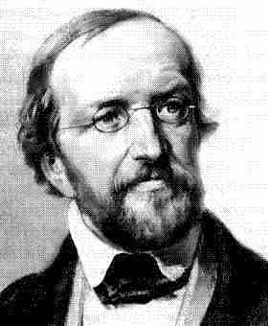
\includegraphics[width=.3\textwidth]{graphics/dirichlet}
%From http://www-gap.dcs.st-and.ac.uk/~history/PictDisplay/Dirichlet.html
\end{center}

\begin{remark}
Theorem~\ref{thm:units} is due to Dirichlet  who lived 1805--1859.
Thomas Hirst described Dirichlet thus:
\begin{quote}He is a rather tall, 
lanky-looking man, with moustache and beard about
to turn grey with a somewhat harsh voice and rather deaf. He was
unwashed, with his cup of coffee and cigar. One of his failings is
forgetting time, he pulls his watch out, finds it past three, and runs
out without even finishing the sentence.
\end{quote}
Koch wrote that:
\begin{quote}
... important parts of mathematics were influenced by Dirichlet. His
proofs characteristically started with surprisingly simple
observations, followed by extremely sharp analysis of the remaining
problem. 
\end{quote}
I think Koch's observation nicely describes the proof we will give of
Theorem~\ref{thm:units}.
\end{remark}



Units have a simple characterization in terms of their norm.
\begin{proposition}\label{prop:unitnorm}\iprop{unit norm characterization}
An element $a\in \O_K$ is a unit if and only if $\Norm_{K/\Q}(a)=\pm 1$.
\end{proposition}
\begin{proof}
Write $\Norm=\Norm_{K/\Q}$.  If $a$ is a unit, then $a^{-1}$ is also a
unit, and $1=\Norm(a)\Norm(a^{-1})$.  Since both $\Norm(a)$ and
$\Norm(a^{-1})$ are integers, it follows that $\Norm(a)=\pm 1$.
Conversely, if $a\in \O_K$ and $\Norm(a)=\pm 1$, then the equation
$aa^{-1}=1=\pm \Norm(a)$ implies that $a^{-1} = \pm \Norm(a)/a$.  But
$\Norm(a)$ is the product of the images of~$a$ in $\C$ by all
embeddings of~$K$ into~$\C$, so $\Norm(a)/a$ is also a product of
images of~$a$ in~$\C$, hence a product of algebraic integers,
hence an algebraic integer.  Thus $a^{-1}\in K\cap \Zbar = \O_K$, 
which proves that~$a$ is a unit.
\end{proof}

\begin{remark}
Proposition~\ref{prop:unitnorm} is false if we replace $\O_K$ by $K$.
For example, if $\alpha$ is a root of $x^2-\frac{1}{2}x+1$, then
$\alpha$ has norm $\pm 1$, but $\alpha$ is not a unit of $\O_K$, since
$\alpha\not\in \O_K$.  To general Proposition~\ref{prop:unitnorm} to an
arbitrary finite extension $R/S$ of Dedekind domains, we replace $\pm
1$ by ``an element of $S^*$''.
\end{remark}

Let $r$ be the number of real and $s$ the number of complex conjugate
embeddings of $K$ into $\C$, so $n=[K:\Q]=r+2s$.
Define the {\em log map}
$$
\vphi:U_K \to \R^{r+s}
$$
by 
$$
 \vphi(a) = (\log|\sigma_1(a)|,\ldots, \log|\sigma_{r+s}(a)|).
$$
(Here $|z|$ is the usual absolute value of $z=x+iy\in\C$, 
so $|z|=\sqrt{x^2+y^2}$.)

\begin{lemma}\label{lem:inh}\ilem{hyperplane embedding}
The image of $\vphi$ lies in the hyperplane 
\begin{equation}\label{eqn:hyperplane}
H = \{(x_1,\ldots, x_{r+s})\in\R^{r+s} : 
  x_1+ \cdots + x_r + 2x_{r+1} + \cdots + 2x_{r+s} = 0\}.
\end{equation}
\end{lemma}
\begin{proof}
If $a\in U_K$, then 
by Proposition~\ref{prop:unitnorm}, 
$$\left(\prod_{i=1}^{r} |\sigma_i(a)|\right) 
  \cdot \left( \prod_{i=r+1}^{r+s} |\sigma_i(a)|^2 \right) = 
|\Norm_{K/\Q}(a)| = 1.$$
Taking logs of both sides proves the lemma.
\end{proof}

\begin{lemma}\label{lem:vphifinitekernel}
The kernel of $\vphi$ is finite.
\end{lemma}
\begin{proof}
We have
\begin{align*}
  \Ker(\vphi) &\subset \{a\in\O_K : |\sigma_i(a)| = 1 \text{ for }i=1,\ldots,r+s\}\\
              &\subset \sigma(\O_K) \cap X,
\end{align*}
where $X$ is the bounded subset of $\R^{r+s}$ of elements all of whose coordinates
have absolute value at most $1$.  Since $\sigma(\O_K)$ is a lattice 
(see Proposition~\ref{prop:ok_lattice}), 
the intersection $\sigma(\O_K)\cap X$ is finite, so $\Ker(\vphi)$ is finite.
\end{proof}

\begin{lemma}\label{lem:kerfcg}
The kernel of~$\vphi$ is a finite cyclic group.
\end{lemma}
\begin{proof}
  Lemma~\ref{lem:vphifinitekernel} implies that $\ker(\vphi)$ is a
  finite group.  It is a general fact that any finite subgroup $G$ of
  the multiplicative group $K^*$ of a field is cyclic.  (Proof: If~$n$
  is the exponent of~$G$, then every element of~$G$ is a root of the
  polynomial $x^n-1$.  A polynomial of degree~$n$ over a field has at
  most~$n$ roots, so $G$ has order at most~$n$, hence~$G$ is cyclic of
  order~$n$.)
\end{proof}

To prove Theorem~\ref{thm:units}, it suffices to prove that
$\Im(\vphi)$ is a lattice in the hyperplane~$H$ of
(\ref{eqn:hyperplane}), which we view as a vector space of dimension
$r+s-1$.

Define an embedding
\begin{equation}\label{eqn:sigma3}
 \sigma : K\hra \R^n
\end{equation}
given by $\sigma(x) = (\sigma_1(x),\ldots,\sigma_{r+s}(x))$,
where we view $\C\isom \R\times \R$ via $a+b i\mapsto (a,b)$.
Thus this is the embedding
\begin{align*}
 x\mapsto \big(&\sigma_1(x), \sigma_2(x),\ldots, \sigma_r(x),\\
     &\quad \Re(\sigma_{r+1}(x)), \Im(\sigma_{r+1}(x)), 
    \ldots, \Re(\sigma_{r+s}(x)), \Im(\sigma_{r+s}(x))\big).
\end{align*}

\begin{lemma}\label{lem:ukdiscrete}
The image $\vphi:U_K\to \R^{r+s}$ is discrete.
\end{lemma}
\begin{proof}
Let $X$ be a bounded subset of $\R^{r+s}$.
We will show that the intersection $\vphi(U_K)\cap X$ is finite.
Since $X$ is bounded, for any $u\in
Y=\vphi^{-1}(X)\subset U_K$ the coordinates of $\sigma(u)$ are bounded, 
since $|\log(x)|$ is bounded on bounded subsets
of $[1,\infty)$.
Thus $\sigma(Y)$ is
a bounded subset of $\R^n$.  Since $\sigma(Y)\subset \sigma(\O_K)$,
and $\sigma(\O_K)$ is a lattice in $\R^n$, it follows that $\sigma(Y)$
is finite; moreover,~$\sigma$ is injective, so $Y$ is finite.
Thus $\vphi(U_K)\cap X \subset \vphi(Y) \cap X$ is finite.
\end{proof}

We will use the following lemma in our
proof of Theorem~\ref{thm:units}.
\begin{lemma}\label{lem:chooseci}
Let $n\geq 2$ be an integer, suppose $w_1,\ldots, w_n\in\R$
are not all equal, and suppose $A, B\in\R$ are positive. Then
there exist $d_1,\ldots, d_{n} \in \R_{>0}$ such that 
$$|w_1\log(d_1)+\cdots +w_{n}\log(d_{n})| > B$$  
and $d_1\cdots d_n = A$.
\end{lemma}
\begin{proof}
Order the $w_i$ so
that $w_1\neq 0$.  By hypothesis there exists a $w_j$ such that
$w_j\neq w_1$, and again re-ordering we may assume that $j=2$.  Set
$d_3=\cdots=d_{r+s}=1$.  Suppose $d_1, d_2$ are any positive real numbers
with  $d_1 d_2 = A$.  Since $\log(1)=0$,
\begin{align*}
  \left|\sum_{i=1}^{n} w_i \log(d_i)\right|
  &= |w_1\log(d_1) + w_2\log(d_2)|\\
  &= |w_1 \log(d_1) + w_2\log(A/d_1)| \\
  &= |(w_1-w_2)\log(d_1) + w_2\log(A)|
\end{align*}
Since $w_1\neq w_2$,  we have $|(w_1-w_2)\log(d_1) + w_2\log(A)|\to\infty$
as $d_1\to \infty$.  It is thus possible to choose the $d_i$ as in the lemma.
\end{proof}

\begin{proof}[Proof of Theorem~\ref{thm:units}]
By Lemma~\ref{lem:ukdiscrete}, the image $\vphi(U_K)$
is discrete, so it remains to show that $\vphi(U_K)$
spans~$H$.  
Let~$W$ be the $\R$-span of the image
$\vphi(U_K)$, and note that~$W$ is a subspace of~$H$,
by Lemma~\ref{lem:inh}.  We will show
that $W=H$ indirectly by showing that if $v\not \in H^{\perp}$,
where~$\perp$ is the orthogonal complement 
with respect to the dot product on $\R^{r+s}$, then
$v\not \in W^{\perp}$.  This will show that $W^{\perp}\subset
H^{\perp}$, hence that $H\subset W$, as required.

Thus suppose $z=(z_1,\ldots,z_{r+s})\not\in H^{\perp}$.  
Define a function $f:K^*\to \R$ by 
\begin{equation}\label{eqn:f}
  f(x) = z_1\log|\sigma_1(x)| + \cdots + z_{r+s}\log|\sigma_{r+s}(x)|.
\end{equation}
Note that $f(U_K)=\{0\}$ if and only if $z\in W^{\perp}$,
so to show that $z\not\in W^{\perp}$ we show that there exists some $u\in
U_K$ with $f(u)\neq 0$.

Let 
$$
  A=\sqrt{|d_K|} \cdot \left( \frac{2}{\pi}\right)^s \in \R_{>0}.
$$
Choose any positive real numbers $c_1,\ldots, c_{r+s} \in \R_{>0}$
such that
$$
  c_1\cdots c_r\cdot (c_{r+1}\cdots c_{r+s})^2 = A.
$$
Let 
\begin{align*}
  S &= \{(x_1,\ldots,x_n) \in \R^n : \\
    &\qquad\qquad |x_i|\leq c_i\text{ for } 1\leq i \leq r,\\
    &\qquad\qquad |x_i^2 + x_{i+s}^2| \leq c_i^2 \text{ for } r<i\leq r+s\} \subset \R^n.
\end{align*}
Then~$S$ is closed, bounded, convex, symmetric with respect to the
origin, and of dimension $r+2s$, since $S$ is a product of~$r$ intervals
and~$s$ discs, each of which has these properties.
Viewing $S$ as a product of intervals and discs, we see that the volume of $S$ is
$$
  \Vol(S) = \prod_{i=1}^r (2c_i) \cdot \prod_{i=1}^s (\pi c_i^2) 
          = 2^r\cdot \pi^s \cdot A
  = 2^{r+s}\sqrt{|d_K|} = 2^n \cdot 2^{-s}\sqrt{|d_K|}.
$$

Recall Blichfeldt's Lemma~\ref{lem:blichfeld}, which asserts  
that if~$L$ is a lattice and~$S$ is closed,
bounded, etc., and has volume at least $2^n\cdot \Vol(V/L)$, then
$S\cap L$ contains a nonzero element.   To apply this lemma, we
take $L=\sigma(\O_K)\subset \R^n$, where $\sigma$ is as in (\ref{eqn:sigma3}).
By Lemma~\ref{lem:volok}, 
we have
$\Vol(\R^n/L) = 2^{-s}\sqrt{|d_K|}$.  To check the hypothesis
of Blichfeld's lemma, note that 
$$
 \Vol(S) = 2^n \cdot 2^{-s} \sqrt{|d_K|} = 2^n \Vol(\R^n/L).
$$
Thus there exists a nonzero element $x$ in $S\cap \sigma(\O_K)$.
Let $a\in \O_K$ with $\sigma(a)=x$, then $\sigma(a)\in S$, so
$|\sigma_i(a)|\leq c_i$ for $1\leq i\leq r+s$.
We then have
\begin{align*}
  |\Norm_{K/\Q}(a)| &=
   \left|\prod_{i=1}^{r+2s} \sigma_i(a)\right|\\
   &=  \prod_{i=1}^r |\sigma_i(a)|\cdot \prod_{i=r+1}^s|\sigma_i(a)|^2\\
   &\leq c_1\cdots c_r\cdot (c_{r+1}\cdots c_{r+s})^2 = A.
\end{align*}
Since $a\in \O_K$ is nonzero, we also have
$$
 |\Norm_{K/\Q}(a)|\geq 1.
$$
Moreover, if for any $i\leq r$, we have $|\sigma_i(a)|< \frac{c_i}{A}$, then 
$$
 1\leq |\Norm_{K/\Q}(a)| < c_1\cdots \frac{c_i}{A}\cdots c_r \cdot (c_{r+1}\cdots c_{r+s})^2 = \frac{A}{A} = 1,
$$
a contradiction, so $|\sigma_i(a)|\geq \frac{c_i}{A}$ for $i=1,\ldots, r$. Likewise,
$|\sigma_i(a)|^2 \geq \frac{c_i^2}{A}$, for $i=r+1,\ldots, r+s$. 
Rewriting this 
we have 
\begin{equation}\label{eqn:cisigbound}
  \frac{c_i}{|\sigma_i(a)|}\leq A\quad\text{ for }i\leq r\quad\text{and}\quad
\left(\frac{c_i}{|\sigma_i(a)|}\right)^2\leq A\quad\text{for } i=r+1,\ldots, r+s.
\end{equation}

Recall that our overall strategy is to use an appropriately chosen~$a$
to construct a unit $u\in U_K$ such $f(u)\neq 0$.  First, let
$b_1,\ldots, b_m$ be representative generators for the finitely many
nonzero principal ideals of $\O_K$ of norm at most $A$.  Since
$|\Norm_{K/\Q}(a)|\leq A$, we have $(a)=(b_j)$, for some $j$, so there
is a unit~$u\in \O_K$ such that $a=u b_j$.

Let 
$$
t = t_{c_1,\ldots, c_{r+s}} = z_1\log(c_1)+\cdots +z_{r+s}\log(c_{r+s}),
$$ 
and recall $f:K^*\to \R$ defined in
(\ref{eqn:f}) above.
We have
\begin{align*}
  |f(u) - t| &= |f(a) - f(b_j) - t|\\
   &\leq |f(b_j)| + |t - f(a)|\\
   &=|f(b_j)| + |z_1(\log(c_1) - \log(|\sigma_1(a)|)) + \cdots + z_{r+s}(\log(c_{r+s}) - \log(|\sigma_{r+s}(a)|))|\\
   &=|f(b_j)| + |z_1\cdot \log(c_1/|\sigma_1(a)|) + \cdots + \frac{z_{r+s}}{2}\cdot \log((c_{r+s}/|\sigma_{r+s}(a)|)^2)|\\
   &\leq |f(b_j)| + \log(A)\cdot\left(\sum_{i=1}^{r}|z_i| + \frac{1}{2}\cdot \sum_{i=r+1}^s|z_i|\right) \defeq B_j.
\end{align*}
In the last step we use (\ref{eqn:cisigbound}).

Let $B=\max_{j} B_j$, and note that $B$ does not depend on the choice
of the $c_i$; in fact, it only depends our {\em fixed} choice of $z$ and on the field $K$.
Moreover, for any choice of the $c_i$ as above, we have
$$
  |f(u) - t| \leq B.
$$
If we can choose positive real numbers~$c_i$ such that
\begin{align*}
 c_1\cdots c_r\cdot (c_{r+1}\cdots c_{r+s})^2 &= A\\
  |t_{c_1,\ldots, c_{r+s}}| &>B,
\end{align*}
then the fact that $|f(u)-t|\leq B$ would then imply that $|f(u)|>0$,
which is exactly what we aimed to prove.

If $r+s=1$, then we are trying to prove that $\vphi(U_K)$ is a lattice
in $\R^0=\R^{r+s-1}$, which is automatically true, so assume $r+s>1$.
To finish the proof, we explain how to use Lemma~\ref{lem:chooseci}
to choose $c_i$ such that $|t|>B$.  We have
\begin{align*}
t &= z_1\log(c_1)+\cdots +z_{r+s}\log(c_{r+s})\\
&= z_1\log(c_1)+\cdots +  z_r\log(c_r)+
\frac{1}{2}\cdot z_{r+1}\log(c_{r+1}^2) + 
\cdots + \frac{1}{2}\cdot z_{r+s}\log(c_{r+s}^2)\\
&=w_1\log(d_1)+\cdots +  w_r\log(d_r)+
w_{r+1}\log(d_{r+1}) + 
\cdots +\cdot w_{r+s}\log(d_{r+s}),
\end{align*}
where $w_i=z_i$ and $d_i=c_i$ for $i\leq r$, and
$w_i=\frac{1}{2}z_i$ and $d_i=c_i^2$ for $r<i\leq r+s$.
The condition that $z\not\in H^{\perp}$ is that the $w_i$ are not all
the same, 
 and in our new coordinates the lemma is equivalent to
showing that $|\sum_{i=1}^{r+s} w_i \log(d_i)|>B$, subject to the
condition that $\prod_{i=1}^{r+s} d_i = A$. 
But this is exactly what Lemma~\ref{lem:chooseci} shows.
It is thus possible
to find a unit~$u$ such that $|f(u)|>0$.  Thus $z\not\in
W^{\perp}$, so $W^{\perp}\subset H^{\perp}$, whence $H\subset W$,
which finishes the proof of Theorem~\ref{thm:units}.
\end{proof}

\section{Examples with Sage}
\subsection{Pell's Equation}\label{sec:pell}
The so-called ``Pell's equation'' is $x^2-dy^2 = 1$ with $d>0$ square
free, and we seek integer solutions $x,y$ to this equation.  If
$x+y\sqrt{d}\in K = \Q(\sqrt{d})$, then
$$
  \Norm(x+y\sqrt{d}) = (x+y\sqrt{d})(x-y\sqrt{d}) = x^2 -dy^2.
$$ 
Thus if $(x,y)$ are integers such that $x^2 - d y^2 = 1$, then $\alpha
= x + \sqrt{d}y \in \O_K$ has norm $1$, so by
Proposition~\ref{prop:unitnorm} we have $\alpha \in U_K$.  The integer
solutions to Pell's equation thus form a finite-index subgroup of the
group of units in the ring of integers of $\Q(\sqrt{d})$.  Dirichlet's
unit theorem implies that for any~$d$ the solutions to Pell's equation
with $x,y$ not both negative forms an infinite cyclic group, which is
a fact that takes substantial work to prove using only elementary
number theory (for example, using continued fractions).

We first solve Pell's equation $x^2 - 5y^2 = 1$ with $d=5$ by finding
the units of the ring of integers of $\QQ(\sqrt{5})$ using Sage.

\begin{lstlisting}
sage: K.<sqrt5> = QuadraticField(5)
sage: G = K.unit_group(); G
Unit group with structure C2 x Z of Number Field in sqrt5 with 
defining polynomial x^2 - 5
sage: G.0
-1
sage: u = G.1; u
1/2*sqrt5 - 1/2
\end{lstlisting}

The subgroup of cubes gives us the units with integer $x,y$ (not both negative).

\begin{lstlisting}
sage: u, u^2, u^3, u^4, u^5, u^6
(1/2*sqrt5 - 1/2, -1/2*sqrt5 + 3/2, sqrt5 - 2, -3/2*sqrt5 + 7/2, 
 5/2*sqrt5 - 11/2, -4*sqrt5 + 9)
sage: [list(v^i) for i in [0..9]]
[[1, 0], [-2, 1], [9, -4], [-38, 17], [161, -72], [-682, 305], [2889, 
 -1292], [-12238, 5473], [51841, -23184], [-219602, 98209]]
\end{lstlisting}

% \begin{verbatim}
%    > R<x> := PolynomialRing(RationalField());
%    > K<a> := NumberField(x^2-5);
%    > G, phi := UnitGroup(K);
%    > G;
%    Abelian Group isomorphic to Z/2 + Z
%    Defined on 2 generators
%    Relations:
%        2*G.1 = 0
%    > K!phi(G.1);
%    -1
%    > u := K!phi(G.2); u;
%    1/2*(a + 1)
%    > u^2;
%    1/2*(a + 3)
%    > u^3;
%    a + 2
%    > Norm(u);
%    -1
%    > Norm(u^3);
%    -1
%    > Norm(u^6);
%    1
%    > fund := u^6;
%    > fund;
%    4*a + 9
%    > 9^2 - 5*4^2;
%    1
%    > fund^2;
%    72*a + 161
%    > fund^3;
%    1292*a + 2889
%    > fund^4;
%    23184*a + 51841
%    > fund^5;
%    416020*a + 930249
% \end{verbatim}

A great article about Pell's equation is \cite{lenstra:pell}.  The
MathSciNet review begins: ``This wonderful article begins with history
and some elementary facts and proceeds to greater and greater depth
about the existence of solutions to Pell equations and then later the
algorithmic issues of finding those solutions. The cattle problem is
discussed, as are modern smooth number methods for solving Pell
equations and the algorithmic issues of representing very large
solutions in a reasonable way.''

The simplest solutions to Pell's equation can be huge, even when~$d$
is quite small.  Read Lenstra's paper for some examples from
over two thousand years ago.  Here is one example for $d=10000019$.

\begin{lstlisting}
sage: K.<a> = QuadraticField(next_prime(10^7))
sage: G = K.unit_group(); G.1
163580259880346328225592238121094625499142677693142915506747253000
340064100365767872890438816249271266423998175030309436575610631639
272377601680603795883791477817611974184075445702823789975945910042
8895693238165048098039*a - 
517286692885814967470170672368346798303629034373575202975075605058
714958080893991274427903448098643836512878351227856269086856679078
304979321047765031073345259902622712059164969008633603603640331175
6634562204182936222240930
\end{lstlisting}

\begin{exercise}
  Let $U$ be the group of units $x+y\sqrt{5}$ of the ring of integers
  of $K=\QQ(\sqrt{5})$.  
\begin{enumerate}
\item Prove that the set $S$ of units $x+y\sqrt{5} \in U$ with
  $x,y\in\ZZ$ is a subgroup of $U$.  (The main point is to show that
  the inverse of a unit with $x,y\in\Z$ again has coefficients in
  $\Z$.)
\item Let $U^3$ denote the subgroup of cubes of elements of $U$.
  Prove that $S=U^3$ by showing that $U^3\subset S \subsetneq U$ and
  that there are no groups $H$ with $U^3\subsetneq H \subsetneq U$.
\end{enumerate}
\end{exercise}

\subsection{Examples with Various Signatures}
In this section we give examples for various $(r,s)$ pairs. 
First we consider $K=\Q(i)$.
\begin{lstlisting}
sage: K.<a> = QuadraticField(-1)
sage: K.signature()
(0, 1)
sage: U = K.unit_group(); U
Unit group with structure C4 of Number Field in a with 
defining polynomial x^2 + 1
sage: U.0
-a
\end{lstlisting}

%    > R<x> := PolynomialRing(RationalField());
%    > K<a> := NumberField(x^2+1);
%    > Signature(K);
%    0 1    // r=0, s=1
%    > G,phi := UnitGroup(K);
%    > G;
%    Abelian Group isomorphic to Z/4
%    Defined on 1 generator
%    Relations:
%        4*G.1 = 0
%    > K!phi(G.1);
%    -a


The {\tt signature} method returns the
number of real and complex conjugate embeddings
of $K$ into $\C$.  The \verb|unit_group| method,
which we used above, returns the unit group $U_K$
as an abstract abelian group and a homomorphism $U_K\to \O_K$.

Next we consider $K=\Q(\sqrt[3]{2})$.
\begin{lstlisting}
sage: R.<x> = QQ[]
sage: K.<a> = NumberField(x^3 - 2)
sage: K.signature()
(1, 1)
sage: U = K.unit_group(); U
Unit group with structure C2 x Z of Number Field in a with 
defining polynomial x^3 - 2
sage: U.gens()
[-1, a - 1]
sage: u = U.1; u
a - 1
\end{lstlisting}

%    > K<a> := NumberField(x^3-2);
%    > Signature(K);
%    1 1
%    > G,phi := UnitGroup(K);
%    > G;
%    Abelian Group isomorphic to Z/2 + Z
%    Defined on 2 generators
%    Relations:
%        2*G.1 = 0
%    > K!phi(G.2);
%    -a + 1


Below we use the \verb|places| command, which returns the real embeddings
and representatives for the complex conjugate embeddings.
We use the places to define the log map $\varphi$, which plays such a big
role in this chapter. 
\begin{lstlisting}
sage: S = K.places(prec=53); S
[Ring morphism:
  From: Number Field in a with defining polynomial x^3 - 2
  To:   Real Double Field
  Defn: a |--> 1.25992104989, Ring morphism:
  From: Number Field in a with defining polynomial x^3 - 2
  To:   Complex Double Field
  Defn: a |--> -0.629960524947 + 1.09112363597*I]
sage: phi = lambda z : [log(abs(sigma(z))) for sigma in S]
sage: phi(u)
[-1.34737734833, 0.673688674165]
sage: phi(K(-1))
[0.0, 0.0]
\end{lstlisting}
Note that $\vphi:U_K \to \R^2$, and the image lands in the
1-dimensional subspace of $(x_1,x_2)$ such that $x_1 +2x_2 = 0$. Also,
note that $\varphi(-1)=0$.

%    > Conjugates(K!phi(G.2));
%    [ -0.25992104989487316476721060727822835057025146470099999999995,
%    1.6299605249474365823836053036391141752851257323513843923104 - 
%    1.09112363597172140356007261418980888132587333874018547370560*i, 
%    1.6299605249474365823836053036391141752851257323513843923104 + 
%    1.09112363597172140356007261418980888132587333874018547370560*i ]
%    > Logs(K!phi(G.2));   // image of infinite order unit -- generates a lattice
%    [ -1.34737734832938410091818789144565304628306227332099999999989\
%    , 0.6736886741646920504590939457228265231415311366603288999999 ]
%    > Logs(K!phi(G.1));   // image of -1
%    [ 0.E-57, 0.E-57 ]

Let's try a field such that $r+s-1=2$.  First, one with $r=0$ and
$s=3$:
\begin{lstlisting}
sage: K.<a> = NumberField(x^6 + x + 1)
sage: K.signature()
(0, 3)
sage: U = K.unit_group(); U
Unit group with structure C2 x Z x Z of Number Field in a with 
defining polynomial x^6 + x + 1
sage: u1 = U.1; u1
a
sage: u2 = U.2; u2
a^3 + a
sage: S = K.places(prec=53)
sage: phi = lambda z : [log(abs(sigma(z))) for sigma in S]
sage: phi(u1)
[-0.167415483286, 0.0486439097527, 0.118771573533]
sage: phi(u2)
[0.306785708923, -1.07251465055, 0.765728941626]
sage: phi(K(-1))
[0.0, 0.0, 0.0]
sage: sum(phi(u1))
-2.63677968348e-15
sage: sum(phi(u2))
-5.10702591328e-15
\end{lstlisting}
%    > K<a> := NumberField(x^6+x+1);
%    > Signature(K);
%    0 3
%    > G, phi := UnitGroup(K);
%    > G;
%    Abelian Group isomorphic to Z/2 + Z + Z
%    Defined on 3 generators
%    Relations:
%        2*G.1 = 0
%    > u1 := K!phi(G.2); u1;
%    a
%    > u2 := K!phi(G.3); u2;
%    -2*a^5 - a^3 + a^2 + a
%    > Logs(u1);
%    [ 0.11877157353322375762475480482285510811783185904379239999998, 
%    0.048643909752673399635150940533329986148342128393119899999997, 
%    -0.16741548328589715725990574535618509426617398743691229999999 ]
%    > Logs(u2);
%    [ 1.6502294567845884711894772749682228152154948421589999999997, 
%    -2.09638539134527779532491660083370951943382108902299999999997, 
%    0.44615593456068932413543932586548670421832624686433469999994 ]

Notice that the log image of $u_1$ is clearly not a real multiple of
the log image of~$u_2$ (e.g., the scalar would have to be positive
because of the first coefficient, but negative because of the second).
This illustrates the fact that the log images of $u_1$ and $u_2$ span
a two-dimensional space.

Next we compute a field with $r=3$ and $s=0$.  (A field with $s=0$
is called totally real.)
\begin{lstlisting}
sage: K.<a> = NumberField(x^3 + x^2 - 5*x - 1)
sage: K.signature()
(3, 0)
sage: U = K.unit_group(); U
Unit group with structure C2 x Z x Z of Number Field in a with 
defining polynomial x^3 + x^2 - 5*x - 1
sage: u1 = U.1; u
a - 1
sage: u2 = U.2; u2
a
sage: S = K.places(prec=53)
sage: phi = lambda z : [log(abs(sigma(z))) for sigma in S]
sage: phi(u1)
[-0.774767022346, -0.392848724581, 1.16761574693]
sage: phi(u2)
[0.996681204093, -1.64022415032, 0.643542946229]
\end{lstlisting}

%    > K<a> := NumberField(x^3 + x^2 - 5*x - 1);
%    > Signature(K);
%    3 0
%    > G, phi := UnitGroup(K);
%    > G;
%    Abelian Group isomorphic to Z/2 + Z + Z
%    Defined on 3 generators
%    Relations:
%        2*G.1 = 0
%    > u1 := K!phi(G.2); u1;
%    1/2*(a^2 + 2*a - 1)
%    > u2 := K!phi(G.3); u2;
%    a
%    > Logs(u1);
%    [ 1.16761574692758757159598251863681302946987760474899999999995, 
%    -0.39284872458139826129179862583435951875841422643044369999996, 
%    -0.7747670223461893103041838928024535107114633783181766999998 ]
%    > Logs(u2);
%    [ 0.6435429462288618773851817227686467257757954024463081999999, 
%    -1.6402241503223171469101505551700850575583464226669999999999, 
%    0.9966812040934552695249688324014383317825510202205498999998 ]

A field with $r=0$ is called totally complex.  For
example, the \defn{cyclotomic fields} $\Q(\zeta_n)$ are totally
complex, where $\zeta_n$ is a primitive $n$th root of 
unity.  The degree of $\Q(\zeta_n)$ over $\Q$ is
$\vphi(n)$ and $r=0$, so $s=\vphi(n)/2$ (assuming $n>2$).
\begin{lstlisting}
sage: K.<a> = CyclotomicField(11); K
Cyclotomic Field of order 11 and degree 10
sage: K.signature()
(0, 5)
sage: U = K.unit_group(); U
Unit group with structure C22 x Z x Z x Z x Z of Cyclotomic Field 
of order 11 and degree 10
sage: u = U.1; u
a^9 + a^7 + a^5 + a^3 + a + 1
sage: S = K.places(prec=20)
sage: phi = lambda z : [log(abs(sigma(z))) for sigma in S]
sage: phi(u)
[1.2566, 0.18533, -0.26981, -0.52028, -0.65179]
sage: for u in U.gens():
...       print phi(u)
[0.00000, 0.00000, 0.00000, -9.5367e-7, -9.5367e-7]
[1.2566, 0.18533, -0.26981, -0.52028, -0.65179]
[0.26981, 0.52029, -0.18533, 0.65180, -1.2566]
[0.65180, 0.26981, -1.2566, -0.18533, 0.52028]
[-0.084484, -1.1721, -0.33496, 0.60477, 0.98675]
\end{lstlisting}

%    > K := CyclotomicField(11); K;
%    Cyclotomic Field of order 11 and degree 10
%    > G, phi := UnitGroup(K);
%    > G;
%    Abelian Group isomorphic to Z/22 + Z + Z + Z + Z
%    Defined on 5 generators
%    Relations:
%        22*G.1 = 0
%    > u := K!phi(G.2); u;
%    zeta_11^9 + zeta_11^8 + zeta_11^7 + zeta_11^6 + zeta_11^5 + 
%        zeta_11^3 + zeta_11^2 + zeta_11 + 1
%    > Logs(u);
%    [ -1.25656632417872848745322215929976803991663080388899999999969,
%    0.6517968940331400079717923884685099182823284402303273999999, 
%    -0.18533004655986214094922163920197221556431542171819269999999, 
%    0.5202849820300749393306985734118507551388955065272236999998, 
%    0.26981449467537568109995283662137958205972227885009159999993 ]
%    > K!phi(G.3);
%    zeta_11^9 + zeta_11^7 + zeta_11^6 + zeta_11^5 + zeta_11^4 + 
%        zeta_11^3 + zeta_11^2 + zeta_11 + 1
%    > K!phi(G.4);
%    zeta_11^9 + zeta_11^8 + zeta_11^7 + zeta_11^6 + zeta_11^5 + 
%        zeta_11^4 + zeta_11^3 + zeta_11^2 + zeta_11
%    > K!phi(G.5);
%    zeta_11^9 + zeta_11^8 + zeta_11^7 + zeta_11^6 + zeta_11^5 + 
%        zeta_11^4 + zeta_11^2 + zeta_11 + 1

How far can we go computing unit groups of cyclotomic fields
directly with Sage?
\begin{lstlisting}
sage: time U = CyclotomicField(11).unit_group()
Time: CPU 0.13 s, Wall: 0.13 s
sage: time U = CyclotomicField(13).unit_group()
Time: CPU 0.24 s, Wall: 0.24 s
sage: time U = CyclotomicField(17).unit_group()
Time: CPU 0.98 s, Wall: 0.98 s
sage: time U = CyclotomicField(23).unit_group()
.... I waited a few minutes and gave up....
\end{lstlisting}

However, if you are willing to assume some conjectures (something
related to the Generalized Riemann Hypothesis), you can go further:
\begin{lstlisting}
sage: proof.number_field(False)
sage: time U = CyclotomicField(11).unit_group()
CPU times: user 0.08 s, sys: 0.00 s, total: 0.09 s
Wall time: 0.09 s
sage: time U = CyclotomicField(13).unit_group()
CPU times: user 0.11 s, sys: 0.00 s, total: 0.12 s
Wall time: 0.12 s
sage: time U = CyclotomicField(17).unit_group()
CPU times: user 0.52 s, sys: 0.00 s, total: 0.53 s
Wall time: 0.53 s
sage: time U = CyclotomicField(23).unit_group()
CPU times: user 2.42 s, sys: 0.02 s, total: 2.44 s
Wall time: 2.44 s
sage: time U = CyclotomicField(29).unit_group()
CPU times: user 21.07 s, sys: 1.06 s, total: 22.13 s
Wall time: 22.14 s
\end{lstlisting}
The generators of the units for $\Q(\zeta_{29})$ are
\begin{align*}
u_{0} &= -\zeta_{29}^{3}\\
u_{1} &= \zeta_{29}^{26} + \zeta_{29}^{25} + \zeta_{29}^{22} + \zeta_{29}^{21} + \zeta_{29}^{19} + \zeta_{29}^{18} + \zeta_{29}^{15} + \zeta_{29}^{14} + \zeta_{29}^{11} + \zeta_{29}^{8} + \zeta_{29}^{7} + \zeta_{29}^{4} + \zeta_{29}^{3} + \zeta_{29} + 1\\
u_{2} &= \zeta_{29}^{14} + \zeta_{29}^{3}\\
u_{3} &= \zeta_{29}^{3} + 1\\
u_{4} &= \zeta_{29}^{26} + \zeta_{29}^{20} + \zeta_{29}^{3}\\
u_{5} &= \zeta_{29}^{22} + \zeta_{29}^{11} + \zeta_{29}^{2}\\
u_{6} &= \zeta_{29}^{10} + \zeta_{29}^{9} + \zeta_{29}^{8}\\
u_{7} &= \zeta_{29}^{23} + \zeta_{29}\\
u_{8} &= \zeta_{29}^{17} + \zeta_{29}^{11}\\
u_{9} &= \zeta_{29}^{22} + \zeta_{29}^{3}\\
u_{10} &= \zeta_{29}^{24} + \zeta_{29}^{19} + \zeta_{29}^{5} + 1\\
u_{11} &= \zeta_{29}^{19} + \zeta_{29}^{6}\\
u_{12} &= \zeta_{29}^{27} + \zeta_{29}^{19} + \zeta_{29}^{11} + \zeta_{29}^{6} + \zeta_{29}^{3}\\
u_{13} &= \zeta_{29}^{26} + \zeta_{29}^{15} + \zeta_{29}^{4}\\
\end{align*}

There are better ways to compute units in cyclotomic fields than to
just use general purpose software. For example, there are explicit
{\em cyclotomic units} that can be written down and generate a finite
subgroup of $U_K$. See \cite[Ch.~8]{washington:cyclo}, which would be
a great book to read now that you've got this far in the present book.
Also, using the theorem explained in that book, it is probably
possible to make the \verb|unit_group| command in Sage for cyclotomic
fields extremely fast, which would be an interesting project for a
reader who also likes to code.


%%% Local Variables: 
%%% mode: latex
%%% TeX-master: "ant"
%%% End: 

\chapter{Decomposition and Inertia Groups}
In this chapter we will study extra structure in the case when~$K$
is Galois over~$\Q$.   We will learn about Frobenius elements,
the Artin symbol, decomposition groups, and how the Galois group of
$K$ is related to Galois groups of residue class fields.  These are
the basic structures needed to attach $L$-function to representations of
$\Gal(\Qbar/\Q)$, which will play a central role in the next few
chapters.


\section{Galois Extensions}
In this section we give a survey (no proofs) of the basic facts about
Galois extensions of $\Q$ that will be needed in the rest of this
chapter.
\begin{definition}[Galois]
  An extension $K/L$ of number fields is \defn{Galois} if $$\#\Aut(K/L)
  = [K:L],$$ where $\Aut(K/L)$ is the group of automorphisms of $K$
  that fix $L$.  We write $$\Gal(K/L) = \Aut(K/L).$$
\end{definition}
For example, if $K\subset \C$ is a number field embedded in the complex numbers,
then $K$ is \defn{Galois} over $\QQ$ if
every field homomorphism $K\to \C$ has image $K$.
As another example, any quadratic extension
$K/L$ is Galois over $L$, since it is of the form $L(\sqrt{a})$, for some $a\in
L$, and the nontrivial automorphism is induced by $\sqrt{a}\mapsto
-\sqrt{a}$, so there is always one nontrivial automorphism.  If $f\in
L[x]$ is an irreducible cubic polynomial, and $a$ is a root of $f$,
then one proves in a course on Galois theory that $L(a)$ is Galois
over $L$ if and only if the discriminant of~$f$ is a perfect square
in~$L$.  ``Random'' number fields of degree bigger than $2$ are rarely
Galois.


If $K\subset \C$ is a number field, then the \defn{Galois closure} $K^{\gc}$
of $K$ in $\C$ is the field generated by all images of~$K$ under all
embeddings in~$\C$ (more generally, if $K/L$ is an extension, the
Galois closure of $K$ over $L$ is the field generated by images of
embeddings $K\to \C$ that are the identity map on $L$).  If $K=\Q(a)$,
then $K^{\gc}$ is the field generated by all of the conjugates of~$a$, and is
hence Galois over~$\Q$, since the image under an embedding of any
polynomial in the conjugates of~$a$ is again a polynomial in
conjugates of $a$.


How much bigger can the degree of $K^{\gc}$ be as compared to the
degree of $K=\Q(a)$? There is an embedding of
$\Gal(K^{\gc}/\Q)$ into the group of permutations of the conjugates of
$a$.  If $a$ has~$n$ conjugates, then this is an embedding
$\Gal(K^{\gc}/\Q)\hra S_n$, where $S_n$ is the symmetric group on~$n$
symbols, which has order~$n!$.  Thus the degree of the $K^{\gc}$ over~$\Q$
is a divisor of $n!$. Also $\Gal(K^{\gc}/\Q)$ is a transitive
subgroup of $S_n$, which constrains the possibilities further.  When
$n=2$, we recover the fact that quadratic extensions are Galois.  When
$n=3$, we see that the Galois closure of a cubic extension is either
the cubic extension or a quadratic extension of the cubic extension.
One can show that the Galois closure of a cubic extension is obtained
by adjoining the square root of the discriminant, which is why an
irreducible cubic defines a Galois extension if and only if the discriminant
is a perfect square.


For an extension
$K$ of $\QQ$ of degree $5$, it is ``frequently'' the case that the Galois
closure has degree $120$, and in fact it is an
interesting problem to enumerate examples of degree~$5$ extension in which
the Galois closure has degree smaller than $120$.
For example, the only possibilities for the order of a transitive proper subgroup
of $S_5$ are $5$, $10$, $20$, and $60$; there are also
proper subgroups of $S_5$ order $2, 3, 4, 6, 8, 12$, and $24$, but none
are transitive.

Let $n$ be a positive integer.  Consider the field $K=\Q(\zeta_n)$,
where $\zeta_n=e^{2\pi i/n}$ is a primitive $n$th root of unity.  If
$\sigma:K\to \C$ is an embedding, then $\sigma(\zeta_n)$ is also an
$n$th root of unity, and the group of $n$th roots of unity is cyclic,
so $\sigma(\zeta_n) = \zeta_n^m$ for some $m$ which is invertible
modulo $n$.  Thus $K$ is Galois and $\Gal(K/\Q)\hra (\Z/n\Z)^*$.
However, $[K:\Q]=\vphi(n)$, so this map is an isomorphism.  (Remark:
Taking a limit using the maps $\Gal(\Qbar/\Q)\to
\Gal(\Q(\zeta_{p^r})/\Q)$, we obtain a homomorphism $\Gal(\Qbar/\Q)\to
\Z_p^*$, which is called the {\em $p$-adic cyclotomic character}.)

Compositums of Galois extensions are Galois.  For example, the
biquadratic field $K=\Q(\sqrt{5},\sqrt{-1})$ is a Galois
extension of $\Q$ of degree~$4$, which is the compositum
of the Galois extensions $\Q(\sqrt{5})$ and $\Q(\sqrt{-1})$ of $\Q$.

Fix a number field $K$ that is Galois over a subfield
$L$. Then the Galois group $G=\Gal(K/L)$ acts on many
of the object that we have associated to $K$.

\begin{exercise}
	Describe the natural action of $G$ on the following objects:
	\begin{itemize}
		\item The ring of integers $\O_K$
		\item The group units $U_K$
		\item The set of ideals of $\O_K$
		\item The group of fractional ideals of $\O_K$
		\item The class group $\Cl(K)$
		\item The set $S_\p$ of prime ideals lying over a given nonzero
	prime ideal $\p$ of $\O_L$, i.e., the prime divisors of $\p\O_K$
	\end{itemize}
\end{exercise}

In the next section we will be concerned with the action of
$\Gal(K/L)$ on $S_\p$, though actions on each of the other objects,
especially $\Cl(K)$, are also of great interest.  Understanding the
action of $\Gal(K/L)$ on $S_{\p}$ will enable us to associate, in a
natural way, a holomorphic $L$-function to any complex representation
$\Gal(K/L) \to \GL_n(\C)$.

\section{Decomposition of Primes: $efg=n$}
If $I\subset \O_K$ is any ideal in the ring of integers of
a Galois extension $K$ of $\Q$ and $\sigma\in\Gal(K/\Q)$, then
$$
  \sigma(I) = \{\sigma(x) : x \in I\}
$$
is also an ideal of $\O_K$.


Fix a prime $\p\subset \O_K$ and write $\p\O_K = \P_1^{e_1}\cdots
\P_g^{e_g}$, so $S_\p=\{\P_1,\ldots, \P_g\}$.
\begin{definition}[Residue class degree]
Suppose $\P$ is a prime of $\O_K$ lying over $\p$.
Then the \defn{residue class degree} of $\P$ is
$$
   f_{\P/\p} = [\O_K/\P : \O_L/\p],$$
i.e., the degree of the extension of residue class fields.
\end{definition}
If $M/K/L$ is a tower of field extensions and
$\q$ is a prime of $M$ over $\P$, then
$$f_{\q/\p} = [\O_M/\q : \O_L/\p]
=[\O_M/\q : \O_K/\P]\cdot [\O_K/\P : \O_L/\p] =
f_{\q/\P}\cdot f_{\P/\p},$$
so the residue class degree is multiplicative in
towers.

Note that if $\sigma\in\Gal(K/L)$ and $\P\in S_p$, then $\sigma$
induces an isomorphism of finite fields $\O_K/\P\to \O_K/\sigma(\P)$
that fixes the common subfield $\O_L/\p$.  Thus the residue class
degrees of $\P$ and $\sigma(\P)$ are the same.  In fact, much more is
true.
\begin{theorem}\label{thm:transitive}\ithm{transitive Galois action}
Suppose $K/L$ is a Galois extension of number fields,
and let $\p$ be a prime of $\O_L$.  Write
$\p\O_K=\prod_{i=1}^g \P_i^{e_i}$, and let $f_i = f_{\P_i/\p}$.
Then
$G=\Gal(K/L)$ acts transitively on the set
$S_\p$ of primes $\P_i$, and
$$
  e_1=\cdots =e_g, \qquad f_1 =\cdots = f_g.
$$
Morever, if we let $e$ be the common value of the $e_i$,
$f$ the common value of the $f_i$, and $n=[K:L]$, then
$$
   efg=n.
$$
\end{theorem}
\begin{proof}
For simplicity, we will give the proof only in the case $L=\Q$, but
the proof works in general.  Suppose $p\in\Z$ and
$p\O_K=\p_1^{e_1}\cdots \p_g^{e_g}$, and $S=\{\p_1,\ldots, \p_g\}$.  We
will first prove that $G$ acts transitively on $S$.  Let $\p=\p_i$ for
some~$i$.   Recall Lemma~\ref{lem:magica} which we proved long ago using the
Chinese Remainder Theorem (Theorem~\ref{thm:crt}). It showed there exists
$a\in\p$ such that $(a)/\p$ is an integral ideal that is
coprime to $p\O_K$.   The product
\begin{equation}\label{eqn:prodquo}
 I= \prod_{\sigma\in G} \sigma((a)/\p)
   = \prod_{\sigma\in G} \frac{(\sigma(a))\O_K}{\sigma(\p)}
    = \frac{(\Norm_{K/\Q}(a))\O_K}{\displaystyle \prod_{\sigma\in G} \sigma(\p)}
\end{equation}
is a nonzero integral $\O_K$ ideal since it is a product of nonzero
integral $\O_K$ ideals.
Since $a\in \p$ we have that
$\Norm_{K/\Q}(a) \in \p\cap\Z=p\Z$.  Thus the numerator of
the rightmost expression in (\ref{eqn:prodquo}) is
divisible by $p\O_K$.   Also, because $(a)/\p$ is coprime
to $p\O_K$, each $\sigma((a)/\p)$ is coprime to $p\O_K$
as well.   Thus $I$ is coprime to $p\O_K$.   This means the
denominator of the rightmost expression in (\ref{eqn:prodquo})
must also be divisible by $p\O_K$ in order to cancel the $p\O_K$
in the numerator.  Thus we have shown that for any~$i$,
$$
  \prod_{j=1}^g \p_j^{e_j} = p\O_K \,\,\Big|\,\, \prod_{\sigma\in G} \sigma(\p_i).
$$
By unique factorization, since every $\p_j$ appears in the left hand
side, we must have that for each~$j$ there is a~$\sigma$ with
$\sigma(\p_i)=\p_j$, i.e., $G$ acts transitively on $S$.

Choose some $j$ and suppose that $k\neq j$ is another index.  Because
$G$ acts transitively, there exists $\sigma\in G$ such that
$\sigma(\p_k)=\p_j$.  Applying $\sigma$ to the factorization $p\O_K =
\prod_{i=1}^g \p_i^{e_i}$, we see that
$$\prod_{i=1}^g \p_i^{e_i} = \prod_{i=1}^g \sigma(\p_i)^{e_i}.$$
Using unique factorization,
we get $e_j = e_k$.  Thus $e_1=e_2=\cdots = e_g$.

As was mentioned right before the statement of the theorem,  for any $\sigma\in G$
we have $\O_K/\p_i\isom \O_K/\sigma(\p_i)$. Since $G$ acts transitively
it follows that $f_1=f_2=\cdots = f_g$.
We have, upon applying the Chinese Remainder Theorem
and noting $\#(\O_K/(\p^m)) = \#(\O_K/\p)^m$
(see Exercise~\ref{ex:residuefieldofpower}), that
\begin{align*}
[K:\Q]&= \dim_{\Z} \O_K = \dim_{\F_p} \O_K/p\O_K\\
    &= \dim_{\F_p} \left(\bigoplus_{i=1}^g \O_K/\p_i^{e_i}\right)
    = \sum_{i=1}^g e_i f_i
    = efg,
\end{align*}
which completes the proof.
\end{proof}

The rest of this section illustrates the theorem for quadratic fields
and a cubic field and its Galois closure.

\subsection{Special Cases}

\subsubsection*{Quadratic Extensions}

Suppose $K/\Q$ is a quadratic field.  Then $K$ is Galois, so for each prime $p\in\Z$ we have
$2=efg$. There are exactly three possibilities:
\begin{description}
\item[\bf{Ramified:}] $e=2$, $f=g=1$: The prime $p$ \emph{ramifies} in
$\O_K$, which means $p\O_K = \p^2$.  Let $\alpha$ be a generator for $\O_K$ and
$h\in\Z[x]$ a minimal polynomial for $\alpha$.
By Theorem~\ref{thm:fac1} a prime $p$ is ramified in $\O_K$ if and only if
$h$ has a double root modulo~$p$, which is equivalent to $p$ dividing
the discriminant of $h$. This shows there are only finitely many ramified
primes. More generally, the ramified primes are exactly the
ones that divide the discriminant (see \cite[Thm.~24]{marcus1977number}
or
\cite[Cor.~III.2.12]{neukirch1999}).

\item[\bf{Inert}:] $e=1$, $f=2$, $g=1$: The prime $p$ is \emph{inert} in $\O_K$,
which means $p\O_K = \p$ is prime.  It is a nontrivial theorem that
this happens half of the time,
as we will see illustrated below for a particular example.

\item[\bf{Split:}] $e=f=1$, $g=2$: The prime $p$ \emph{splits} in $\O_K$,
which means $p\O_K = \p_1\p_2$ with $\p_1\neq \p_2$.  This happens the other
half of the time.
\end{description}

\begin{example}\label{exam:decompQsqrt5}
Let $K=\Q(\sqrt{5})$, so $\O_K=\Z[\gamma]$, where
$\gamma=(1+\sqrt{5})/2$.  Then $p=5$ is ramified, since $5\O_K =
(\sqrt{5})^2$.  More generally, the order $\Z[\sqrt{5}]$ has index $2$
in $\O_K$, so for any prime $p\neq 2$ we can determine the
factorization of $p$ in $\O_K$ by finding the factorization of the
polynomial $x^2-5\in \F_p[x]$.  The polynomial $x^2-5$ splits as a
product of two distinct factors in $\F_p[x]$ if and only if $e=f=1$
and $g=2$.  For $p\neq 2,5$ this is the case if and only if $5$ is a
square in $\F_p$, i.e., if $\kr{5}{p} = 1$, where $\kr{5}{p}$ is $+1$
if $5$ is a square mod $p$ and $-1$ if $5$ is not.  By quadratic
reciprocity,
$$
 \kr{5}{p} = (-1)^{\frac{5-1}{2}\cdot \frac{p-1}{2}} \cdot \kr{p}{5} =
   \kr{p}{5} = \begin{cases} +1 & \text{ if } p\con \pm 1\pmod{5}\\ -1&\text{ if } p \con \pm 2\pmod{5}.\end{cases}
$$
Thus whether $p$ splits or is inert in
$\O_K$ is determined by the residue class of~$p$
modulo $5$.  It is a theorem of Dirichlet, which was massively
generalized by Chebotarev, that $p\con \pm 1$ half the time
and $p \con \pm 2$ the other half the time.\footnote{
For a technical statement and proof of this theorem,
see \cite{neukirch1999} Theorem~VII.13.4.}
\end{example}

\subsubsection*{The Cube Root of Two}

Suppose $K/\Q$ is not Galois.
Then $e_i$, $f_i$, and~$g$ are defined for each prime $p\in\Z$,
but we need not have $e_1=\cdots=e_g$ or $f_1=\cdots =f_g$.  We do still have that
$\sum_{i=1}^g e_i f_i = n$, by the Chinese Remainder Theorem.
For a proof of this identity, see \cite[Thm.~21]{marcus1977number},
or, for a slightly more general version, \cite[Prop.~I.8.2]{neukirch1999}

Consider the case where $K=\Q(\sqrt[3]{2})$. We know that $\O_K = \Z[\sqrt[3]{2}]$.  Thus
$2\O_K = (\sqrt[3]{2})^3$, so for $2$ we have $e=3$ and $f=g=1$.

Working modulo $5$ we have
$$
 x^3 - 2 = (x+2)(x^2+3x+4) \in \F_5[x],
$$
and the quadratic factor is irreducible.  Thus
$$
 5\O_K = (5, \crtwo+2)\cdot (5, \crtwo^2 + 3\crtwo + 4).
$$
Thus here $g=2$, $e_1=e_2=1$, $f_1=1$, and $f_2=2$.
Thus when $K$ is not Galois we need not have that the $f_i$
are all equal.

\subsection{Definitions and Terminology}

In the previous sections we used words like ``ramify'',
``inert'', and ``split'' to describe the decomposition
of a prime in an extension. This section will define
the generalizations of these concepts which will be used
in later sections.

Let $K/L$ be an extension of number fields. Let
$\O_K,\O_L$ denote the respective ring of integers
and $\q$ a prime in $\O_L$. By Theorem~\ref{thm:intuniqfac} we
know that the ideal $\q\O_K$ factors uniquely into a product
of primes $\p_i$ in $\O_K$ given by
$$
\q\O_K = \p_1^{e_1}\cdots\p_g^{e_g}.
$$
Let $f_i$ be the degree of the extension of
residue fields, i.e.,
$$
f_i = [\O_K/\p_i : \O_L/\q].
$$

\begin{definition}\label{def:ramify}
	The prime $\q$ \emph{ramifies} in $L$
	if $e_i>1$ for some $1\leq i\leq g$.
	Otherwise $\q$ is \emph{unramified}.
	%in geneal, residue fields should be separable, neukrich 49
	If $\q$ is ramified and moreover $f_i=1$
	for all $i$, then $\q$ is \emph{totally ramified}.
\end{definition}

\begin{definition}\label{def:inert}
	The prime $\p$ is \emph{inert} in $L$
	if $\p\O_L$ is prime. In this case we have $g=1$,
	$\q_1=\p\O_L$, and $e_1=1$.
\end{definition}

\begin{definition}\label{def:split}
	The prime $\p$ is \emph{split} in $L$
	if $g>1$. If moreover $g = [L : K]$, then
	$\p$ \emph{splits completely} or is
	\emph{totally split}.
\end{definition}

It will sometimes be helpful to emphasize which prime we are
referring to. To do this we will use the notation $e(\p/\q)$
to represent the power of $\p$ appearing in the
factorization of $\q\O_K$. The number $e(\p/\q)$ is called the
\emph{ramification index} of $\p$ over $\q$.
In this notation we could write $\q\O_K = \prod \p^{e(\p/\q)}$
where the product ranges over all primes $\p$ in $\O_K$.
We will similarly denote $f(\p/\q)$ to be the degree of the extension
of residue fields $[\O_K/\p:\O_L/\q]$. The number $f(\p/\q)$ is called
the \emph{inertia degree} of $\p/\q$. Because the number of primes
over $\q$ depends on the field $K$, we sometimes denote $g$ by $g_K(\q)$.

\begin{exercise}\label{ex:ramificationmultiplicative}
The following are some basic properties of decompositions.
For each one, compare the result with previous examples
we have seen such as Example~\ref{exam:decompQsqrt5}.

Let $K/L/\Q$ be a tower of number fields. Let $p$ be a prime
in $\Z$, $\q$ a prime in $\O_L$ lying over $p$, and $\p$ a prime
in $\O_K$ lying over $\q$.
\begin{enumerate}
	\item[(a)] Show that $e$ is multiplicative, that is $e(\p/p)=e(\p/\q) \cdot e(\q/p)$.
	\item[(b)] Show that $f$ is multiplicative, that is $f(\p/p)=f(\p/\q) \cdot f(\q/p)$.
	\item[(c)] Let $g_L(p)$ be the number of primes of $\O_L$ lying over $p$.
	Show that $g_K(p) = \sum\limits_{\q \text{ lies over } p} g_L(\q)$.
\end{enumerate}
\end{exercise}

\begin{exercise}[See {\cite[Ch.~4, Excercise~24]{marcus1977number}}]
Continue the notation from the previous exercise.
\begin{enumerate}
	\item[(a)]
	If $p$ it totally ramified in $K$
	then it is totally ramified in $L$.

	\item[(b)]
	Let $K'$ be another extension of $L$.
	If $\p$ is totally ramified in $K$ and unramified in $K'$
	then $K\cap K' = L$.
\end{enumerate}

\end{exercise}

\section{The Decomposition Group}
Suppose $K$ is a number field that is Galois over $\Q$ with
group $G=\Gal(K/\Q)$.
Fix a prime $\p\subset \O_K$ lying over $p\in\Z$.
\begin{definition}[Decomposition group]\label{def:decomp}
The \defn{decomposition group} of $\p$ is the subgroup
$$
  D_\p = \{\sigma \in G : \sigma(\p)=\p\} \subset G.
$$
\end{definition}
Note that $D_\p$ is the stabilizer of $\p$ for
the action of $G$ on the set of primes lying over $p$.

It also makes sense to define decomposition groups for relative
extensions $K/L$, but for simplicity and to fix ideas in this section
we only define decomposition groups for a Galois extension $K/\Q$.

Let $k_\p = \O_K/\p$ denote the residue class field of $\p$.
In this section we will prove that there is an exact sequence
$$
  1\to I_\p \to D_\p \to \Gal(k_{\p}/\F_p)\to 1,
$$
where $I_\p$ is the \defn{inertia subgroup} of $D_\p$, and
$\#I_\p=e = e(\p/p)$.
The most interesting part of the proof is
showing that the natural map $D_\p\to  \Gal(k_{\p}/\F_p)$
is surjective. We will also discuss the structure of $D_\p$ and introduce
Frobenius elements, which play a crucial role in understanding Galois
representations.


Recall from Theorem~\ref{thm:transitive}
that~$G$ acts transitively on the set of primes~$\p$ lying
over~$p$.  The orbit-stabilizer theorem implies that $[G:D_\p]$ equals the cardinality of the
orbit of~$\p$, which by Theorem~\ref{thm:transitive}
equals the number~$g$ of primes lying over~$p$, so $[G:D_\p]=g$.

\begin{lemma}\label{decompGpsConj}\ilem{decomposition groups are conjugate}
The decomposition subgroups $D_\p$ corresponding to primes $\p$
lying over a given $p$ are all conjugate as subgroups of~$G$.
\end{lemma}
\begin{proof}
See Exercise~\ref{ex:decompGpsConj}.
\end{proof}

\begin{exercise}\label{ex:decompGpsConj}
Prove Lemma~\ref{decompGpsConj}.

Hint: For $\sigma,\tau\in G$ you need to show $\tau D_\p \tau^{-1} = D_{\tau\p}$.
Start by writing down what it means for $\sigma\in D_\p$
and $\tau\sigma\tau^{-1}\in D_{\tau\p}$.

%solution:
%We have for each $\sigma, \tau \in G$, that
%$$\tau^{-1}\sigma \tau\p = \p
%\iff
%\sigma\tau \p = \tau \p,
%$$
%so
%$$
%\sigma \in D_{\tau\p} \iff \tau^{-1}\sigma\tau\in D_\p.
%$$
%Thus
%$$
% \sigma \in D_\p \iff \tau \sigma \tau^{-1} \in D_{\tau \p},
%$$
%which shows $\tau D_{\p}\tau^{-1} = D_{\tau \p}$.
\end{exercise}

The decomposition group is useful because it allows us
to refine the extension $K/\Q$ into a tower of extensions, such that at
each step in the tower we understand the splitting behavior
of the primes lying over~$p$.


Recall the correspondence between subgroups of the Galois group
$G$ and subfields of $K$. The fixed fields corresponding to the
decomposition and inertia subgroups have an important description
in terms of the splitting behavior of the prime $\p$.
We characterize the fixed field of $D=D_\p$ as follows.

\begin{proposition}\label{prop:nosplit}\iprop{fixed field characterization}
The fixed field
$$K^D=\{a \in K : \sigma(a) = a\text{ for all }
\sigma \in D\}$$
of $D$
is the smallest subfield $L\subset K$ such that
the prime ideal $\q = \p\cap\O_L$
has $g_K(\q)=1$, i.e., there is a unique
prime of $\O_K$ lying over $\q$.
\end{proposition}
\begin{proof}
First suppose $L=K^D$, and note that by Galois theory $\Gal(K/L)\isom
D$, and by Theorem~\ref{thm:transitive}, the group $D$
acts transitively on the primes of $K$ lying over $\q$.  One of
these primes is $\p$, and $D$ fixes $\p$ by definition, so there is
only one prime of $K$ lying over $\q$, that is $g=1$.
Conversely, if $L\subset K$ is such that $\q$
has $g=1$, then $\Gal(K/L)$ fixes $\p$ (since it is the only
prime over $\q$), so $\Gal(K/L)\subset D$, hence $K^D\subset L$.
\end{proof}

Thus $p$ does not split in going from $K^D$ to $K$---it does some
combination of ramifying and staying inert.  To fill in more of
the picture, the following proposition asserts that $p$ splits
completely and does not ramify in $K^D/\Q$.

\begin{proposition}\label{prop:noresidue}\iprop{$e$, $f$, $g$}
Fix a finite Galois extension~$K$ of~$\Q$,
let~$\p$ be a prime lying over~$p$ with decomposition group~$D$,
and set $L=K^D$ and $\q = \p \cap \O_L$.
Then $e(\q/p)=f(\q/p)=1$, $g_L(p)=[L : \Q]$, $e(\p/p)=e(\p/\q)$ and $f(\p/p)=f(\p/\q)$.
\end{proposition}
\begin{proof}
As mentioned right after Definition~\ref{def:decomp}, the
orbit-stabilizer theorem implies that $g_K(p)=[G:D]$, and
by Galois theory $[G:D]=[L:\Q]$, so $g_K(p) = [L:\Q]$. By
Proposition~\ref{prop:nosplit}, we have $g_K(\q)=1$ so
by Theorem~\ref{thm:transitive},
\begin{align*}
	e(\p/\q) \cdot f(\p/\q) = [K:L]
	&=\frac{[K:\Q]}{[L:\Q]} \\
	&= \frac{e(\p/p)\cdot f(\p/p) \cdot g_K(p)}{[L:\Q]}
	\\
	&= e(\p/p)\cdot f(\p/p).
\end{align*}
Now $e(\p/\q)\leq e(\p/p)$ and $f(\p/\q)\leq f(\p/p)$, so
we must have $e(\p/\q)=e(\p/p)$ and $f(\p/\q)=f(\p/p)$.
Since from Exercise~\ref{ex:ramificationmultiplicative} we have
$e(\p/p)=e(\p/\q)\cdot e(\q/p)$ and $f(\p/q)=f(\p/\q)\cdot f(\q/p)$,
it follows that $e(\q/p)=f(\q/p) = 1$.
\end{proof}

\noindent
We summarize the results of the decomposition of a prime
in the tower $K \supseteq L = K^D \supseteq \Q$ in
Table~\ref{tbl:decompfield}. This table shows the ramification
indices, inertia degrees, and the number of primes at each step
of the tower.

\begin{table}[h!]
\centering
\begin{tabular}{ >{$}c<{$} >{$}c<{$} >{$}c<{$} | >{$}c<{$} >{$}c<{$} }
	\text{Ramification ($e$)} & \text{Inertia ($f$)} & \text{Splitting ($g$)} & \text{Primes} & \text{Fields} \\
	\hline
	 &  &  & \p & K \\
	e(\p/p) & f(\p/p) & 1 & \vert & \vert \\
	 &  &  & \q & L \\
	1 & 1 & [L:\Q] & \vert & \vert \\
	 &  &  & p &  \Q
\end{tabular}
\caption{Decomposition in the fixed field $L=K^D$.}
\label{tbl:decompfield}
\end{table}

\subsection{Galois groups of finite fields}\label{sec:galoisfinite}

Each $\sigma\in D=D_\p$ acts in a well-defined
way on the finite field $k_{\p} = \O_K/\p$, so we obtain
a homomorphism
$$
  \vphi:D_\p \to \Aut(k_{\p}/\F_p).
$$
We pause for a moment and review a few basic properties of
extensions of finite fields. In particular, they turn out
to be Galois so the map $\vphi$ above is actually a map
$D_\p \to \Gal(k_{\p}/\F_p)$.
The properties in this section are general properties
of Galois groups for finite fields.

\begin{definition}
	Let $k$ be any field of characteristic $p$.
	Define $\Frob_p:k\to k$ to be the homomorphism
	given by $a\mapsto a^p$. The map $\Frob_p$ is
	called the \emph{Frobenius} homomorphism.
\end{definition}

\begin{exercise}\label{ex:frob}
\hfill
\begin{enumerate}
	\item[(a)]
	Show the map $\Frob_p$ is in fact a field homomorphism,
	that is $\Frob_p(a + b) = \Frob_p(a) + \Frob_p(b)$
	and $\Frob_p(ab) = \Frob_p(a)\Frob_p(b)$.
	
	\item[(b)]
	Suppose $k = \F_p$. Then show $\Frob_p = id$, i.e.,
	$a^p = a$ for any $a\in\F_p$.
	
	\item[(c)]
	Suppose $k = \F_{q}$ where $q=p^f$ for some $f\geq 1$. Show that $\Frob_p:k\to k$ is an automorphism.
	
	\item[(d)]
	Continuing part (c), note that by
	Exercise~\ref{ex:finitesubgroupoffieldcyclic}
	$k^*$ is cyclic. Let $a\in k$ be a generator for
	$k^*$, so $a$ has multiplicative order $p^f-1$ and $k = \F_p(a)$.
	Show that
	$$
	\Frob_p^n(a) = a^{p^n} = a
	\quad\Leftrightarrow\quad
	(p^f - 1) \mid p^n - 1
	\quad\Leftrightarrow\quad
	f \mid n
	$$
\end{enumerate}
\end{exercise}

\begin{remark}
	Exercise~\ref{ex:frob} shows that all finite fields
	are \emph{perfect}. For more on perfect fields see
	a standard abstract algebra text such as
	\cite{dummit2004abstract}.
\end{remark}

By Exercise~\ref{ex:frob}(b,c) the map $\Frob_p$ is an
automorphism of $k_\p$ fixing $\F_p$ and hence defines
an element in $\Gal(k_{\p}/\F_p)$. Let $f = f_{\p/p}$ be the residue
degree of $\p$, i.e., $f = [k_{\p}:\F_p]$.
Exercise~\ref{ex:frob}(d) shows the order of $\Frob_p$ is~$f$.
Since the order of the automorphism group of a field extension
is at most the degree of the extension, we conclude that
$\Aut(k_{\p}/\F_p)$ is generated by $\Frob_p$. This shows
$\Aut(k_{\p}/\F_p)$ has order equal to the degree $[k_{\p}/\F_p]$
so we conclude that $k_{\p}/\F_p$ is Galois.
We summarize the discussion into the following theorem.

\begin{theorem}\label{thm:galoisgroupfinitefield}
	The extension $k_{\p}/\F_p$ is Galois and moreover,
	$\Gal(k_{\p}/\F_p)$ is generated by the Frobenius map
	$\Frob_p$ defined by $a\mapsto a^p$.
\end{theorem}

\begin{exercise}
	Prove that up to isomorphism there is
	exactly one finite field of each degree.
	
	Hint: By Theorem~\ref{thm:galoisgroupfinitefield}
	all elements in a finite field satisfy an equation
	of the form $x^{p^f} - 1$ where $p$ is the
	characteristic and $f$ is the degree over the
	field $\F_p$.
\end{exercise}


\subsection{The Exact Sequence}\label{sec:exactseq}
Because $D_\p$ preserves $\p$, there is a natural reduction homomorphism
$$
  \vphi:D_\p \to \Gal(k_{\p}/\F_p).
$$
\begin{theorem}\label{thm:redsurj}\ithm{reduction of Galois group}
The homomorphism $\vphi$ is surjective.
\end{theorem}
\begin{proof}
Let $D = D_\p$ and $\tilde{a} \in  k_{\p}$ be an element such that $ k_{\p} = \F_p(\tilde{a})$.
Lift $\tilde{a}$ to an algebraic integer $a\in \O_K$, and let
$h=\prod_{\sigma\in {D}}(x-\sigma(a))\in K^D[x]$.
Let $\tilde{h}$ be the reduction of $h$ modulo~$\p$.
Note that $h(a) = 0$ so $\tilde{h}(\tilde{a}) = 0$.

Note that the coefficients of $h$ lie in $\O_{K^D}$.
By Proposition~\ref{prop:noresidue}, the residue field of $\O_{K^D}$
is $\F_p$ so $\tilde{h}\in\F_p[x]$.
Therefore $\tilde{h}$ is a multiple of the minimal polynomial of
$\tilde{a}$ over $\F_p$. In particular, $\Frob_p(\tilde{a})$
must also be a root of $\tilde{h}$.
Since the roots of $\tilde{h}$ are of the form
$\widetilde{\sigma(a)}$ this shows that
$\widetilde{\sigma(a)} = \Frob(\tilde{a})$ for some $\sigma\in D$.
Hence $\varphi(\sigma)(\tilde{a}) = \Frob(\tilde{a})$. Since elements
of $\Gal(K_\p/\F_p)$ are determined by their action on $\tilde{a}$
by choice of $\tilde{a}$, it follows that $\vphi(\sigma) = \Frob$
and hence $\varphi$ is surjective because $\Frob_p$
generates $\Gal(k_\p/\F_p)$.
\end{proof}

\begin{definition}[Inertia Group]
The \defn{inertia group associated to
 $\p$} is the kernel $I_\p$ of $D_\p\to\Gal(k_{\p}/\F_p)$.
\end{definition}
We have an exact sequence of groups
\begin{equation}\label{eqn:exact}
   1 \to I_\p \to D_\p \to \Gal(k_{\p}/\F_p)\to 1.
\end{equation}
The inertia group is a measure of how $p$ ramifies in $K$.
\begin{corollary}\icor{order of inertia group}
We have $\# I_\p = e = e(\p/p)$.
\end{corollary}
\begin{proof}
The exact sequence (\ref{eqn:exact}) implies that
$\#I_\p = \#D_\p / f$ where $f = f(\p/p) = [k_\p : \F_p]$.
Applying Propositions~\ref{prop:nosplit} and \ref{prop:noresidue}, we have
$$\#D_\p = [K:L] = \frac{[K:\Q]}{g} = \frac{efg}{g} = ef.$$
Dividing both sides by $f$ proves the corollary.
\end{proof}

We have the following characterization of $I_\p$.
\begin{proposition}\label{prop:charip}\iprop{inertia group characterization}
Let $K/\Q$ be a Galois extension with group $G$,
and let~$\p$ be a prime of $\O_K$ lying
over a prime~$p$.  Then
$$
I_\p = \{\sigma\in G \, :\, \sigma(a) \equiv a\pmod{\p}\text{ for all } a\in\O_K\}.
$$
\end{proposition}
\begin{proof}
  By definition $I_\p = \{\sigma\in D_\p : \sigma(a) \equiv
  a\pmod{\p}\text{ for all } a\in\O_K\}$, so it suffices to show that
  if $\sigma\not\in D_\p$, then there exists $a\in\O_K$ such that
  $\sigma(a)\not\con a\pmod{\p}$.  If $\sigma\not\in D_\p$, then
  $\sigma^{-1}\not\in D_\p$, so $\sigma^{-1}(\p)\neq \p$.  Since both
  are maximal ideals, there exists $a\in\p$ with
  $a\not\in\sigma^{-1}(\p)$, i.e., $\sigma(a)\not\in\p$.  Thus
  $\sigma(a)\not\con a\pmod{\p}$.
\end{proof}

%\begin{figure}\label{fig}
%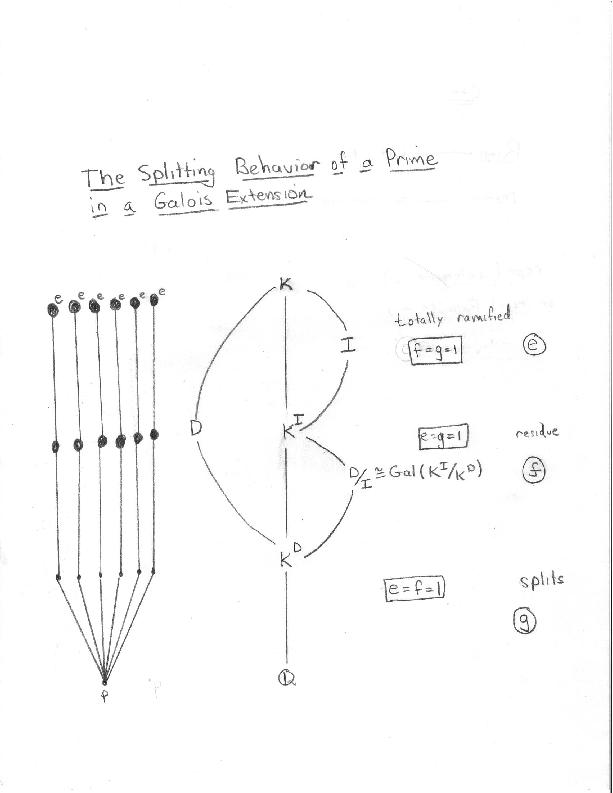
\includegraphics[width=\textwidth]{splitting}
%\caption{The Splitting of Behavior of a Prime in a Galois Extension}
%\end{figure}


\section{Frobenius Elements}

Suppose that $K/\Q$ is a finite Galois extension with group $G$ and
$p$ is a prime such that $e=1$ (i.e., an unramified prime).  Then
$I=I_\p=1$ for any $\p\mid p$, so the map $\vphi$ of
Theorem~\ref{thm:redsurj}
is a canonical isomorphism $D_\p \isom \Gal( k_{\p}/\F_p)$.
By Section~\ref{sec:galoisfinite},
the group $\Gal( k_{\p}/\F_p)$ is
cyclic with canonical generator $\Frob_p$.
The \defn{Frobenius element} corresponding to $\p$ is
$\Frob_\p\in D_\p$. It is the unique (see Exercise~\ref{ex:frobunique})
element of $G$ such that for all
$a\in\O_K$ we have
$$
  \Frob_\p(a)\con a^p\pmod{\p}.
$$


\begin{exercise}\label{ex:frobunique}
	With the notation above, prove that $\Frob_\p$ is
	unique. That is, if $\sigma$ satisfies
	$\sigma(a) \equiv a^p \pmod{\p}$ for all $a\in\O_K$
	then $\sigma = \Frob_\p$.

	Hint: First show $\sigma\in D_\p$, %TODO turn this into an environment
	then argue as in the proof of Proposition~\ref{prop:charip}.
\end{exercise}


Just as the primes $\p$ and decomposition groups $D_\p$ are all
conjugate, the Frobenius elements corresponding to primes
$\p\mid p$ are all conjugate as elements of~$G$.

\begin{proposition}\iprop{conjugation of Frobenius}
For each $\sigma \in G$, we have
$$
 \Frob_{\sigma\p} = \sigma\Frob_\p\sigma^{-1}.
$$
In particular, the Frobenius elements lying over a given
prime are all conjugate.
\end{proposition}
\begin{proof}
Fix $\sigma\in G$. For any $a\in\O_K$ we have
$\Frob_\p(\sigma^{-1}(a)) - \sigma^{-1}(a)^p \in \p$.
Applying~$\sigma$ to both sides, we see that
$\sigma\Frob_\p(\sigma^{-1}(a)) - a^p \in \sigma\p$,
so $\sigma\Frob_\p\sigma^{-1} = \Frob_{\sigma \p}$.
\end{proof}

Thus the conjugacy class of $\Frob_\p$ in $G$ is a well-defined
function of~$p$.  For example, if $G$ is abelian, then $\Frob_\p$ does
not depend on the choice of $\p$ lying over $p$ and we obtain a well
defined symbol $\kr{K/\Q}{p} =\Frob_\p\in G$ called the \defn{Artin
symbol}.  It extends to a homomorphism from the free abelian
group on unramified primes~$p$ to~$G$.
Class field theory (for~$\Q$) sets up a natural bijection
between abelian Galois extensions of $\Q$ and certain maps from
certain subgroups of the group of fractional ideals for~$\Z$ (i.e., $\Q^*$).
  We have
just described one direction of this bijection, which associates to an
abelian extension the Artin symbol (which is a homomorphism).
The Kronecker-Weber theorem asserts that the abelian extensions of
$\Q$ are exactly the subfields of the fields $\Q(\zeta_n)$, as $n$
varies over all positive integers.  By Galois theory there is a
correspondence between the subfields of the field $\Q(\zeta_n)$,
which has Galois group $(\Z/n\Z)^*$, and the subgroups of $(\Z/n\Z)^*$.
If $H \subseteq (\Z/n\Z)^*$ is the subgroup corresponding to
$K \subset \Q(\zeta_n)$ then the Artin reciprocity map
$p\mapsto \kr{K/\Q}{p}$ is given by $p\mapsto [p]\in (\Z/n\Z)^*/H$.

\begin{remark}
	Notice above that the $n$ used is not unique. That is,
	if~$K$ is an abelian extension of $\Q$ then it lies in some~$\Q(\zeta_n)$.
	But then it also lies inside of~$\Q(\zeta_{dn})$ for any
	positive integer~$d$. However, a different choice of $n$
	would mean a different choice of $H$. Note that the
	quotient $(\Z/n\Z)^*/H$ used is not dependent on $n$
	since it is isomorphic to the Galois group of $K/\Q$.
\end{remark}

\section{The Artin Conjecture}\label{sec:artin}

The Galois group $\Gal(\Qbar/\Q)$ is an object of central importance
in number theory, and we can interpret much of number theory as the
study of this group.  A good way to study a group is to study how it
acts on various objects, that is, to study its representations.

Endow $\galq$ with the topology which has as a basis of open neighborhoods
of the origin the subgroups $\Gal(\Qbar/K)$, where~{$K$ varies
over finite Galois extensions of~$\Q$.
Fix a positive integer~$n$ and let $\GL_n(\C)$ be the group of
$n\times n$ invertible matrices over~$\C$ with the discrete topology.

\begin{warning}\label{warn:galqtopology}
	The topology on $\galq$ is {\bf not} the topology induced
	by taking as a basis of open neighborhoods around the origin
	the collection of finite-index normal subgroups of $\galq$,
	see \cite[Ch.~7]{milne:FT} or
	Exercise~\ref{ex:nonopensbgpfiniteindexgalq}. In particular,
	there exist nonopen normal subgroups of finite index which
	do not correspond to subgroups $\Gal(\Qbar/K)$ for some
	finite Galois extension $K/\Q$.
\end{warning}

\begin{definition}
A \defn{complex  $n$-dimensional representation} of $\galq$
is a continuous homomorphism
$$
  \rho:\galq\to \GL_n(\C).
$$
\end{definition}
For $\rho$ to be continuous means that if $K$ is the fixed
field of $\Ker(\rho)$, then $K/\Q$ is a finite Galois extension.  We have
a diagram
$$\xymatrix{ {\galq}\ar[rr]^{\rho}\ar[dr]& &{\GL_n(\C)}\\
&{\Gal(K/\Q)}\ar@{^{(}->}[ur]_{\rho'}}
$$

\begin{exercise}\label{ex:galqrepfiniteimage}
	Suppose $\rho:\galq\to\GL_n(\C)$ is continuous.
	Show that the image is finite.
\end{exercise}

\begin{remark}
	The converse to Exercise~\ref{ex:galqrepfiniteimage}
	is \textbf{false} in general (see
	Exercise~\ref{ex:nonopensbgpfiniteindexgalq}).
	This is essentially the same warning as
	\ref{warn:galqtopology}, however it is worth
	pointing out to avoid mistakes.
	\footnote{See \cite[pg.~1]{artinconjectureLectureNotes}.}
\end{remark}

\begin{exercise}\label{ex:nonopensbgpfiniteindexgalq}
	Find a nonopen subgroup of index $2$ in $\galq$.
	Note this is also an example of a non-continuous
	homomorphism $\galq\to\GL_n(\C)$ with finite image.
	
	
	Hint: Use Zorn's lemma to show that there are homomorphisms
	$\galq\to\{\pm 1\}$ with finite image that are not continuous,
	since they do not factor through the Galois group of any finite
	Galois extension.
	
	More hints: The extension $\Q(\sqrt{d}, d \in \Q^*/(\Q^*)^2)$
	is an extension of~$\Q$ with Galois group $X\ncisom \prod \F_2$.
	The index-two open subgroups of~$X$ correspond to the quadratic
	extensions of~$\Q$. However, Zorn's lemma implies that~$X$
	contains many index-two subgroups that do not correspond to
	quadratic extensions of~$\Q$.
\end{exercise}

Fix a Galois representation~$\rho$ and let $K$ be the fixed field of
$\ker(\rho)$, so~$\rho$ factors through $\Gal(K/\Q)$.  For each prime
$p\in\Z$ that is not ramified in $K$, there is an element
$\Frob_\p\in\Gal(K/\Q)$ that is well-defined up to conjugation by
elements of $\Gal(K/\Q)$.  This means that $\rho'(\Frob_p)\in
\GL_n(\C)$ is well-defined up to conjugation.  Thus the characteristic
polynomial $F_p(x)\in\C[x]$ of $\rho'(\Frob_p)$ is a well-defined
invariant of $p$ and $\rho$.  Let
$$R_p(x) = x^{\deg(F_p)}\cdot F_p(1/x) = 1 + \cdots +
\det(\Frob_p)\cdot x^{\deg(F_p)}$$
be the polynomial obtain
by reversing the order of the coefficients of $F_p$.
Following E.~Artin \cite{artin:conjecture, artin:conjecture2}, set
\begin{equation}\label{eqn:artin}
L(\rho,s) = \prod_{p\text{ unramified}}
\frac{1}{R_p(p^{-s})}.
\end{equation}
We view $L(\rho,s)$ as a function of a single complex variable $s$.
One can prove that $L(\rho,s)$ is holomorphic on some right
half plane, and extends to a meromorphic function on all $\C$.
\begin{conjecture}[Artin]\label{conj:artin}
The $L$-function of any continuous representation $$\Gal(\Qbar/\Q)\to\GL_n(\C)$$
is an entire function on all $\C$, except possibly at $1$.
\end{conjecture}
This conjecture asserts that there is some way to analytically continue
$L(\rho,s)$ to the whole complex plane, except possibly at $1$.
(A standard fact from complex analysis is that this analytic
continuation must be unique.)
The simple pole at $s=1$ corresponds to the trivial representation (the
Riemann zeta function), and if $n\geq 2$ and $\rho$ is irreducible,
then the conjecture is that $\rho$ extends to a holomorphic function
on all $\C$.

The conjecture is known when $n=1$.  Assume for the rest of this
paragraph that $\rho$ is odd, i.e., if $c\in\Gal(\Qbar/\Q)$ is complex
conjugation, then $\det(\rho(c))=-1$.  When $n=2$ and the image of
$\rho$ in $\PGL_2(\C)$ is a solvable group, the conjecture is known,
and is a deep theorem of Langlands and others (see
\cite{langlands:basechange}), which played a crucial roll in Wiles's
proof of Fermat's Last Theorem.  When $n=2$ and the image of $\rho$ in
$\PGL_2(\C)$ is not solvable, the only possibility is that the
projective image is isomorphic to the alternating group~$A_5$.
Because~$A_5$ is the symmetry group of the icosahedron, these
representations are called \defn{icosahedral}.  In this case, Joe
Buhler's Harvard Ph.D. thesis \cite{buhler:thesis} gave the first
example in which $\rho$ was shown to satisfy
Conjecture~\ref{conj:artin}.  There is a book \cite{mr95i:11001},
which proves Artin's conjecture for 7 icosahedral representation (none
of which are twists of each other).  Kevin Buzzard and the author
proved the conjecture for 8 more examples \cite{buzzard-stein:artin}.
Subsequently, Richard Taylor, Kevin Buzzard, Nick Shepherd-Barron, and
Mark Dickinson proved the conjecture for an infinite class of
icosahedral Galois representations (disjoint from the examples)
\cite{bdsbt}.  The general problem for $n=2$ is in fact now completely
solved, due to recent work of Khare and Wintenberger
\cite{khare-wintenberger:serre1} that proves Serre's conjecture.

%%% Local Variables:
%%% mode: latex
%%% TeX-master: "ant"
%%% End:

\chapter[Elliptic Curves and $L$-functions]{Elliptic Curves, Galois Representations, and $L$-functions}

This chapter is about elliptic curves and the central role they play
in algebraic number theory.  Our approach will be less systematic and
more a survey than most of the rest of this book.  The goal is to
give you a glimpse of the forefront of research by assuming many basic
facts that can be found in other books (see, e.g.,
\cite{silverman:aec}).

\section{Groups Attached to Elliptic Curves}


\begin{definition}[Elliptic Curve]\label{defn:ec}
  An \defn{elliptic curve} over a field~$K$ is a genus one curve~$E$
  defined over~$K$ equipped with a distinguished point $\O \in E(K)$.
  Here $E(K)$ is the set of all points on $E$ defined over $K$.
\end{definition}
We will not define \emph{genus} in this book, except to note that a
nonsingular curve over~$K$ has genus one if and only if over~$\Kbar$
it can be realized as a nonsingular plane cubic curve.\footnote{
	For a detailed and technical explanation of genus
	see \cite[Ch.~II.8]{hartshorne} or
	\cite[Ch.~7.3]{liu2006algebraic}
}
Moreover, one
can show (using the Riemann-Roch formula) that over any field a genus
one curve with a rational point can always be defined by a projective
cubic equation of the form
$$
  Y^2 Z + a_1 XYZ + a_3 YZ^2  = X^3  + a_2 X^2Z + a_4 XZ^2 + a_6 Z^3.
$$
In this form the distinguished point $\O$ is $(X:Y:Z) = (0:1:0)$.
Note that $\O$ is the only point on the curve with $Z=0$. So we
can consider the rest of the curve in the affine coordinates
by projecting onto the affine plane defined by $Z\neq 0$.
This gives the equation
\begin{equation}\label{weq}
  y^2 +a_1 xy + a_3 y = x^3 + a_2 x^2 + a_4 x + a_6.
\end{equation}
Thus one often presents an elliptic curve by giving a {\em Weierstrass
  equation} (\ref{weq}), though there are significant computational
advantages to other equations for curves (e.g., Edwards coordinates --
see work of Bernstein and Lange in \cite{bernstein2007inverted}).

Using \sage we plot an elliptic curve over the finite field
$\F_7$ and an elliptic curve curve defined over $\Q$.
\begin{sagecode} %skip
\begin{sagecell}
E = EllipticCurve(GF(7), [1,0])
E
\end{sagecell}
\begin{sageout}
Elliptic Curve defined by y^2 = x^3 + x over
    Finite Field of size 7
\end{sageout}
\end{sagecode}
\begin{sagecode}
\begin{sagecell}
E.plot(pointsize=60, gridlines=True)
\end{sagecell}
\begin{sageout}[escapechar=!]
!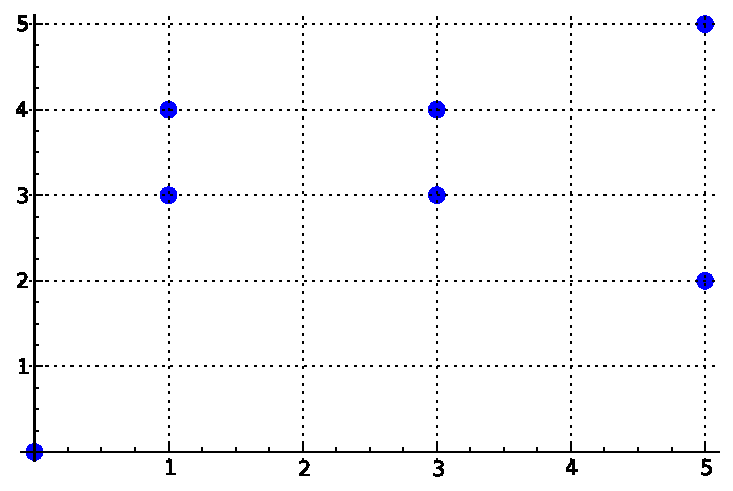
\includegraphics[width=0.9\textwidth]{graphics/ecmod7}
\end{sageout}
\end{sagecode}

\begin{sagecode} %skip
\begin{sagecell}
E = EllipticCurve([1,0])
E
\end{sagecell}
\begin{sageout}
Elliptic Curve defined by y^2 = x^3 + x over
    Rational Field
\end{sageout}
\end{sagecode}
\begin{sagecode}
\begin{sagecell}
E.plot()
\end{sagecell}
\begin{sageout}[escapechar=!]
!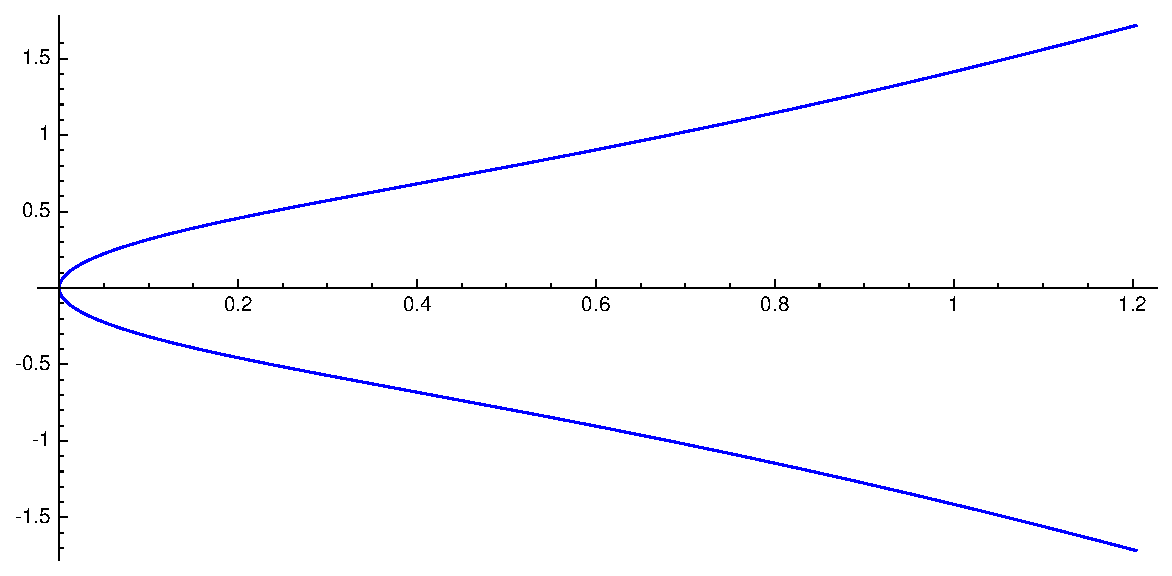
\includegraphics[width=0.9\textwidth]{graphics/ecq}
\end{sageout}
\end{sagecode}

Note that both plots above are of the affine equation $y^2 = x^3 + x$,
and do not include the distinguished point $\O$, which lies at
infinity.

\begin{remark}
The command {\tt{EllipticCurve}} in \sage
can take as input a list {\tt{[a4,a6]}}
of coefficients and returns an elliptic curve given
by a Weirstrass equation with $a_1=a_2=a_3=0$ and
$a_4,a_6$ as specified.
\end{remark}

\subsection{Abelian Groups Attached to Elliptic Curves}
If $E$ is an elliptic curve over~$K$, then we give the set
$E(K)$ of all $K$-rational points on~$E$ the structure of abelian
group with identity element~$\O$.\footnote{
As a reminder, we will not give rigorous proofs of any facts in
this section. For a more detailed and technical explanation of
the group structure for elliptic curves
see \cite[Ch.~III.2]{silverman:aec}.
}
If we embed $E$ in the projective
plane, then this group is determined by the condition that three
points sum to the zero element $\O$ if and only if they lie on a
common line (some care needs to be taken when the points are not
distinct). In our affine picture, a line will intersect the point
at infinity if it is vertical, or equivalently if it of the form
$x=a$ for some fixed $a\in K$.


\begin{example}\label{ex:ecgplaw}
On the curve $y^2=x^3-5x+4$, we have $(0,2) + (1,0) = (3,4)$.
This is because $(0,2)$, $(1,0)$, and $(3,-4)$ are on a common line
(given by the equation $y = 2 - 2x$) hence they sum to zero:
$$
  (0,2) + (1,0) + (3,-4) = \O.
$$
Notice $(3,4)$, $(3,-4)$, and $\O$ (the point at infinity on the curve) are also
on a common line (given by $x = 3$), so $(3,4)=-(3,-4)$.
We can illustration this in \sage:
\begin{sagecode}
\begin{sagecell}
E = EllipticCurve([-5,4])
E(0,2) + E(1,0)
\end{sagecell}
\begin{sageout}
(3 : 4 : 1)
\end{sageout}
\end{sagecode}
\begin{sagecode}
\begin{sagecell} %skip

G = E.plot()
G += points ([(0,2) , (1,0) , (3,4) , (3,-4)],
    pointsize=90 , color='red', zorder=10)
G += line ([(-1,4) , (4,-6)] , color='black')
G += line ([(3,-6) , (3,6)] , color='black')
G.show()
\end{sagecell}
\begin{sageout}[escapechar=!] %skip
!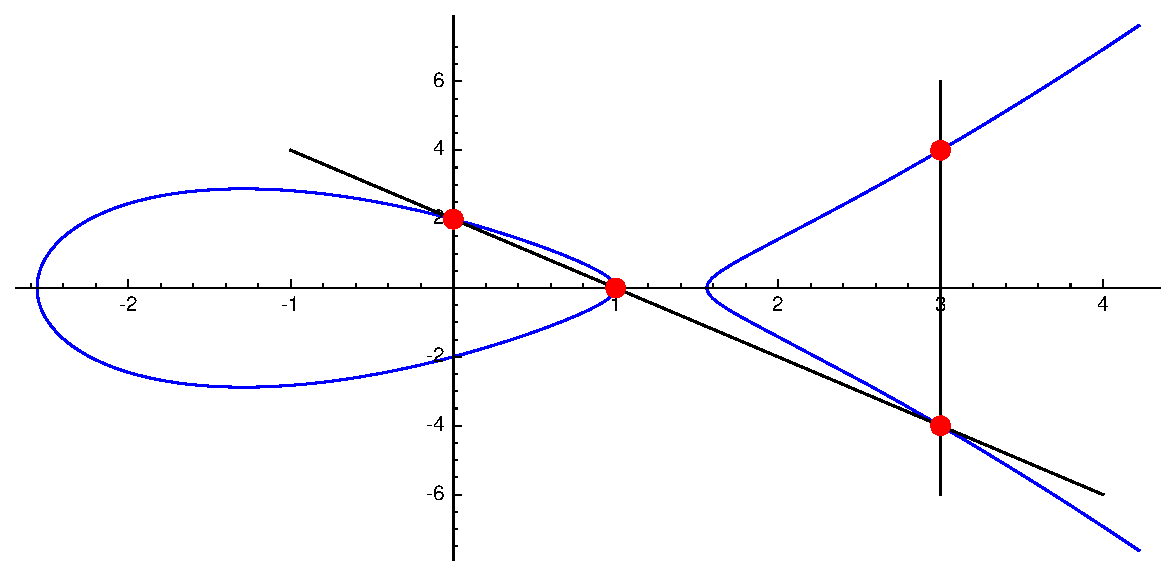
\includegraphics[width=0.925\textwidth]{graphics/grouplaw}
\end{sageout}
\end{sagecode} %link

\noindent
Iterating the group operation often leads quickly to
very complicated points:

\begin{sagecode} %link
\begin{sagecell}
7*E(0,2)
\end{sagecell}
\begin{sageout}
(14100601873051200/48437552041038241 :
-17087004418706677845235922/10660394576906522772066289 :
 1)
\end{sageout}
\end{sagecode}
\end{example}

\begin{remark}
In the previous example we saw that iterating the
group operation led to points which used a lot of digits
to write down. This notion can be made formal and is called
the \emph{height} of the point. The height function is used
to prove the general Mordell-Weil theorem, see
\cite[Ch.~VIII.4]{silverman:aec}
\end{remark}

\begin{exercise}\label{ex:ec2torsion}
	Let $E$ be an elliptic curve given by a
	Weirstrass equation such as (\ref{weq}).
	Show that the points of order two are exactly
	the points on $E$ with $y$-coordinate equal to
	$0$.

	\begin{hint}
		Recall that a point $P$ has order $2$ if
		$P + P + \O = \O$, which means the tangent line
		at $P$ goes through the point at infinity.
	\end{hint}
\end{exercise}

That the above condition---three points on a line sum to
zero---defines an abelian group structure on $E(K)$ is not obvious.
Depending on your perspective, the trickiest part is seeing that the
operation satisfies the associative axiom.  The best way to understand
the group operation on $E(K)$ is to view $E(K)$ as being related to a
class group.  As a first observation, note that the ring
$$
 R = K[x,y]/(y^2 +a_1 xy + a_3 y - (x^3 + a_2 x^2 + a_4 x + a_6))
$$
is a Dedekind domain, so $\Cl(R)$ is defined, and every nonzero
fractional ideal can be written uniquely in terms of prime ideals.
When $K$ is a perfect field, the prime ideals correspond to the Galois
orbits of affine points of $E(\overline{K})$.
Note that these do not include the point at infinity.

Let $\Div(E/K)$ be the free abelian group on the Galois orbits of
points of~$E(\overline{K})$, which as explained above is analogous to
the group of fractional ideals of a number field (here we {\em do}
include the point at infinity).
We call the elements of $\Div(E/K)$
{\em divisors}.  Let $\Pic(E/K)$ be the quotient of $\Div(E/K)$ by the
\emph{principal divisors}, i.e., the divisors associated to rational functions
$f\in K(E)^*$ via
$$
 f \mapsto (f) = \sum_{P} \ord_P(f) [P].
$$
Here $K(E)$ is the fraction field of the ring $R$ defined above.
Note that the principal divisor associated to $f$ is analogous to the
principal fractional ideal associated to a nonzero element of a number
field.  The definition of $\ord_P(f)$ is analogous to the ``power
of~$P$ that divides the principal ideal generated by~$f$''.
%TODO reference text for this? Hartshorne abstract non-singular curves
%TODO or somewhere in Silverman Ch VIII? or an algebra text on
%TODO valuations? or an exercise?
Define the \emph{class group} $\Pic(E/K)$ to be the quotient of the
divisors by the principal divisors, so we have
an exact sequence:
$$
  1\to K(E)^*/K^* \to \Div(E/K) \to \Pic(E/K) \to 0.
$$
%TODO is the 1 - ... - 0 weird?

A key difference between elliptic curves and algebraic number fields
is that the principal divisors in the context of elliptic curves all
have degree~$0$, i.e., the sum of the coefficients of the
divisor~$(f)$ is always~$0$.  This might be a familiar fact to you:
the number of zeros of a nonzero rational function on a projective
curve equals the number of poles, counted with multiplicity.  If we
let $\Div^0(E/K)$ denote the subgroup of divisors of degree~$0$, then
we have an exact sequence
$$
  1\to K(E)^*/K^* \to \Div^0(E/K) \to \Pic^0(E/K) \to 0.
$$

To connect this with the group law on $E(K)$, note that there
is a natural map
$$
 E(K) \to \Pic^0(E/K), \qquad P \mapsto [P-\O].
$$
Using the Riemann-Roch theorem, one can prove that this map
is a bijection, which is moreover an isomorphism of abelian groups.
Thus really when we discuss the group of $K$-rational
points on an $E$, we are talking
about the class group $\Pic^0(E/K)$.

Recall that we proved (Theorem~\ref{thm:finiteclassgrp}) that the
class group $\Cl(\O_K)$ of a number field is finite.
The  group $\Pic^0(E/K) =E(K)$ of an elliptic curve can be
either finite (e.g., for $y^2 + y = x^3 - x + 1$) or infinite (e.g.,
for $y^2 + y = x^3 - x$), and determining which is the case for any particular
curve is one of the central unsolved problems in number theory.

The Mordell-Weil theorem (see Chapter~\ref{ch:weakmw}) asserts that if $E$ is
an elliptic curve over a number field $K$, then there is a nonnegative integer
$r$, referred to as the \emph{algebraic rank of $E$}, such that
\begin{equation}\label{eqn:mw}
  E(\Q) \ncisom \Z^r \oplus T,
\end{equation}
where $T$ is a finite group.   This is similar to Dirichlet's unit theorem, which
gives the structure of the unit group of the ring of integers of a number field.
The main difference is that $T$ need not be cyclic, and computing $r$ appears to be
much more difficult than just finding the number of real and complex roots of
a polynomial!

\begin{example}
\sage has algorithms which can compute this rank for us.
For example we can compute the ranks of the curves
$y^2 + y = x^3 - x + 1$ and $y^2 + y = x^3 - x$ respectively.
\begin{sagecode}
\begin{sagecell}
EllipticCurve([0,0,1,-1,1]).rank()
\end{sagecell}
\begin{sageout}
0
\end{sageout}
\begin{sagecell}
EllipticCurve([0,0,1,-1,0]).rank()
\end{sagecell}
\begin{sageout}
1
\end{sageout}
\end{sagecode}
\end{example}

Also, if $L/K$ is an arbitrary extension of fields, and $E$ is an
elliptic curve over~$K$, then there is a natural inclusion
homomorphism $E(K)\hra E(L)$.  Thus instead of just obtaining one group
attached to an elliptic curve, we obtain a whole collection, one for
each extension of~$L$.  Even more generally, if $S/K$ is an arbitrary
scheme, then $E(S)$ is a group, and the association $S\mapsto E(S)$
defines a functor from the category of schemes to the category of
groups.  Thus each elliptic curve gives rise to map:
$$
 \left\{\text{Schemes over $K$}\right\} \longrightarrow
\left\{\text{Abelian Groups}\right\}
$$

\begin{remark}
	Elliptic curves are not the only objects that induce
	a functor from schemes to groups.
	\emph{Abelian varieties} are a larger class of
	schemes, which includes elliptic curves,
    that also induce such a functor.
    For more on Abelian varieties see
    \cite{milne:abvars}.
\end{remark}

\subsection{A Formula for Adding Points}

We close this section with an explicit formula for
adding two points in $E(K)$.
If $E$ is an elliptic curve over a field $K$,
given by an equation $y^2=x^3+ax+b$, then we
can compute the group addition using the following
algorithm.
\begin{algorithm}[Elliptic Curve Group Law]\label{alg:grouplaw}
Given $P_1, P_2\in E(K)$,
this algorithm computes the sum $R=P_1+P_2 \in E(K)$.
{\sf \begin{enumerate}
\item{}[One Point $\O$] If $P_1=\O$ set $R=P_2$ or if $P_2=\O$ set $R=P_1$
and terminate.  Otherwise write $P_i=(x_i,y_i)$.
\item{}[Negatives]  If $x_1 = x_2$ and $y_1 = -y_2$, set $R=\O$ and terminate.
\item{}[Compute $\lambda$]\label{alg:grouplaw_3}
Set $\ds \lambda = \begin{cases}
 (3x_1^2+a)/(2y_1) & \text{if }P_1 = P_2,\\
(y_1-y_2)/(x_1-x_2) & \text{otherwise.}
\end{cases}$\\
Note: If $y_1=0$ and $P_1=P_2$, output $\O$ and terminate.
\item{}[Compute Sum]\label{alg:grouplaw_4}  Then
$R = \ds \left(\lambda^2 -x_1 - x_2, -\lambda x_3 - \nu\right)$,
where $\nu = y_1 - \lambda x_1$ and~$x_3$ is the~$x$ coordinate of $R$.
\end{enumerate}}
\end{algorithm}

\subsection{Other Groups}
There are other abelian groups attached to elliptic curves, such as
the torsion subgroup $E(K)_{\tor}$ of elements of $E(K)$ of finite
order.  The torsion subgroup is (isomorphic to) the group $T$ that
appeared in Equation~\eqref{eqn:mw} above).  When $K$ is a number
field, there is a group called the Shafarevich-Tate group $\Sha(E/K)$
attached to~$E$, which plays a role similar to that of the class group
of a number field (though it is an open problem to prove that
$\Sha(E/K)$ is finite in general).  The  definition of $\Sha(E/K)$ involves Galois
cohomology, so we wait until Chapter~\ref{ch:gc} to define it.  There
are also component groups attached to~$E$, one for each prime of
$\O_K$.  These groups all come together in the Birch and
Swinnerton-Dyer conjecture (see \url{http://wstein.org/books/bsd/}).

%TODO change this reference please
%TODO is there another book on bsd?

\section[Galois Representations]{Galois Representations Attached to Elliptic Curves}

Let~$E$ be an elliptic curve over a number field~$K$.
In this section we attach representations of
$G_K = \Gal(\Kbar/K)$ to~$E$, and use them to define an $L$-function
$L(E,s)$.   This $L$-function is yet another generalization of the
Riemann Zeta function, that is different from the $L$-functions
attached to complex representations $\Gal(\Qbar/\Q)\to \GL_n(\C)$,
which we encountered before in Section~\ref{sec:artin}.

There is a natural action of $G_K$ on the points of $E(\overline{K})$.
Given a point $P=(a,b)\in E(\overline{K})$ we define $\sigma(P)$ to be
the point $(\sigma(a),\sigma(b))$. Since~$E$ is defined over~$K$ the
point~$\sigma(P)$ will again lie on~$E$ so the action is well
defined. Note that the group structure on~$E$ is defined by
algebraic formulas with coefficients in~$K$. It follows that the
action commutes with point addition meaning that
$\sigma(P+Q) = \sigma(P)+\sigma(Q)$. Now fix an integer $n$.
From what we have seen, the subgroup
$$
E[n] = \{P \in E(\Kbar) : nP = \O\}
$$
is invariant under the action of $G_K$.
We thus obtain a homomorphism
$$
\rhobar_{E,n} : G_K \to \Aut(E[n]).
$$

\begin{warning}
Though the action of $G_K$ leaves the group $E[n]$ fixed,
it may act non-trivially on individual elements! Otherwise
$\rhobar_{E,n}$ would not be very interesting.
\end{warning}

For any positive integer~$n$, the group $E[n]$ is isomorphic as an
abstract abelian group to $(\Z/n\Z)^2$.  There are various
related ways to see why this is true. One is to use the Weierstrass
$\wp$-theory to parametrize $E(\C)$ by the the complex numbers, i.e.,
to find an isomorphism $\C/\Lambda \isom E(\C)$, where $\Lambda$ is a
lattice in $\C$ and the isomorphism is given by $z\mapsto
(\wp(z),\wp'(z))$ with respect to an appropriate choice of coordinates
on $E(\C)$.  It is then an easy exercise to verify that
$(\C/\Lambda)[n]\isom (\Z/n\Z)^2$.
For a detailed and rigorous walk through of this method see
\cite[Ch.~1.4]{diamond-shurman}.

Another way to understand $E[n]$ is to use the fact
that $E(\C)_{\tor}$ is isomorphic
to the quotient
$$\H_1(E(\C),\Q)/\H_1(E(\C),\Z)$$
of homology groups and that the homology of a curve
of genus~$g$ is isomorphic to $\Z^{2g}$.
Then we have a non-canonical isomorphism
$$
 E[n]\approx (\Q/\Z)^2[n] = (\Z/n\Z)^2.
$$

Technically the previous arguments have shown $E(\C)[n] \approx (\Z/n\Z)^2$.
However, our definition of $E[n]$ used points in $E(\overline{K})$.
So we need to show the points $E(\C)[n]$ are actually defined over
$\overline{K}$. Note that $E(\C)[n]$ is finite and invariant under
$\Aut(\C/\overline{K})$ for the same reason as $E[n]$ was invariant under
$\Gal(\overline{K}/K)$ (point addition is defined by algebraic formulas with
coefficients in $K$). It follows that $E(\C)[n]$ is indeed defined over 
$E(\overline{K})$ so the arguments above show that
$E[n] \approx \left(\Z/n\Z\right)^2$.

\begin{remark}
	Notice that the arguments above used many analytic facts about
	geometry over $\C$ (e.g. homology, analytic structure) in order to
	prove algebraic facts (e.g. the number of torsion points) about
	$E(\overline{K})$. This is part of a more general concept called the
	\emph{Lefschetz principle} which generally relates geometry over an
	algebraically closed field of characteristic $0$ to geometry over
	$\C$. For more on this see \cite[Ch.~VI.6]{silverman:aec}.
\end{remark}

\begin{remark}
	In fact, if $p$ is a prime that does not divide $n$
	then $E[n] \approx (\Z/n\Z)^2$ over fields of characteristic
	$p$. However, the methods we used above do not apply
	to the case of positive characteristic. Another method is to
	show the multiplication by $n$ map is separable and has
	degree $n^2$. For a detailed proof see
	\cite[Cor.~III.6.4]{silverman:aec}.
\end{remark}

\begin{exercise}\label{QE[p]finitegaloisext}
	Let $E$ be an elliptic curve defined over a number
	field~$K$. Fix an integer $n$ and consider the
	extension of $K$ given by
	$$
	K(E[n]) = K(\{a,b : (a,b) \in E[n]\}).
	$$
	Show that $K(E[n])/K$ is a finite Galois extension.
	
	Hint: By the arguments above $\#E[n] = n^2$ which shows
	the extension is finite. Next recall that $E[n]$ is left
	invariant by the action of $\Gal(\overline{K}/K)$. What
	can you say about the embeddings from $K(E[n])$ into
	$\overline{K}$ which leave $K$ fixed?
\end{exercise}

\begin{example}
Consider the case when $n=2$. From Exercise~\ref{ex:ec2torsion}
we know that the points in $E[2]$ are exactly the points with
$y$-coordinate $0$. Let $E$ be the elliptic curve given by
$E: y^2 = x^3 + x + 1$. If $y=0$ then $x$ has to be a root
of the polynomial $x^3 + x + 1$, so the points in $E[2]$
are defined over the splitting field of $x^3 + x + 1$.
We can compute these points in \sage.

\begin{sagecode}
\begin{sagecell}
E = EllipticCurve([1,1]); E
\end{sagecell}
\begin{sageout}
Elliptic Curve defined by y^2 = x^3 + x + 1 over
    Rational Field
\end{sageout}
\begin{sagecell}
R.<x> = QQ[]; R
\end{sagecell}
\begin{sageout}
Univariate Polynomial Ring in x over Rational Field
\end{sageout}
\end{sagecode} %link
\begin{sagecode} %link
\begin{sagecell}
f = x^3 + x + 1
K.<a> = NumberField(f)
M.<b> = K.galois_closure(); M
\end{sagecell}
\begin{sageout}
Number Field in b with defining polynomial
    x^6 + 6*x^4 + 9*x^2 + 31
\end{sageout}
\end{sagecode} %link
\begin{sagecode} %link
\begin{sagecell}
F = E.change_ring(M)
T = F.torsion_subgroup(); T
\end{sagecell}
\begin{sageout}
Torsion Subgroup isomorphic to Z/2 + Z/2 associated
    to the Elliptic Curve defined by y^2 = x^3 + x + 1
    over Number Field in b with defining polynomial
    x^6 + 6*x^4 + 9*x^2 + 31
\end{sageout}
\end{sagecode} %link
\begin{sagecode} %link
\begin{sagecell}
T.gens()
\end{sagecell}
\begin{sageout}
((1/18*b^4 + 5/18*b^2 + 1/2*b + 2/9 : 0 : 1),
    (1/18*b^4 + 5/18*b^2 - 1/2*b + 2/9 : 0 : 1))
\end{sageout}
\end{sagecode}
\noindent
Note that this matches with what we expected: we computed
two generators for $E[2]$ (the output of the last cell)
corresponding to two generators of $\left(\Z/2\Z\right)^2$.

\end{example}

If $n=p$ is a prime, then upon chosing a basis for the two-dimensional
$\F_p$-vector space $E[p]$, we obtain an isomorphism $\Aut(E[p]) \isom
\GL_2(\F_p)$.  We thus obtain a mod~$p$ Galois representation
$$
 \rhobar_{E,p} : G_K \to \GL_2(\F_p).
$$
This representation $\rhobar_{E,p}$ is continuous if $\GL_2(\F_p)$ is endowed with the
discrete topology, because the field $K(E[p])$
is a Galois extension of~$K$ of finite degree
by Exercise~\ref{QE[p]finitegaloisext}.

In order to attach an $L$-function to $E$, one could try to embed
$\GL_2(\F_p)$ into $\GL_2(\C)$ and use the construction of Artin
$L$-functions from Section~\ref{sec:artin}.
Unfortunately, this approach is doomed in general, since
$\GL_2(\F_p)$ frequently does not embed in $\GL_2(\C)$.
The following Sage session shows that for $p=5,7$, there are
no 2-dimensional irreducible representations of $\GL_2(\F_p)$,
so $\GL_2(\F_p)$ does not embed in $\GL_2(\C)$.
The notation in the output below is
{\tt [degree of rep, number of times it occurs]}.
\begin{sagecode}
\begin{sagecell}
GL(2,GF(2)).gap().CharacterTable().CharacterDegrees()
\end{sagecell}
\begin{sageout}
[ [ 1, 2 ], [ 2, 1 ] ]
\end{sageout}
\begin{sagecell}
GL(2,GF(3)).gap().CharacterTable().CharacterDegrees()
\end{sagecell}
\begin{sageout}
[ [ 1, 2 ], [ 2, 3 ], [ 3, 2 ], [ 4, 1 ] ]
\end{sageout}
\begin{sagecell}
GL(2,GF(5)).gap().CharacterTable().CharacterDegrees()
\end{sagecell}
\begin{sageout}
[ [ 1, 4 ], [ 4, 10 ], [ 5, 4 ], [ 6, 6 ] ]
\end{sageout}
\begin{sagecell}
GL(2,GF(7)).gap().CharacterTable().CharacterDegrees()
\end{sagecell}
\begin{sageout}
[ [ 1, 6 ], [ 6, 21 ], [ 7, 6 ], [ 8, 15 ] ]
\end{sageout}
\end{sagecode}

Instead of using the complex numbers, we use the
\emph{$p$-adic numbers}\footnote{
For a review of $p$-adic numbers and $p$-adic analysis
see \cite{koblitz1996p}.
}, as
follows.  For each power $p^m$ of $p$, we have defined a homomorphism
$$
  \rhobar_{E,p^m}: G_K \to \Aut(E[p^m]) \ncisom \GL_2(\Z/p^m\Z).
$$
We combine together all of these representations (for all $m\geq 1$)
using the inverse limit.
Recall that the $p$-adic numbers are
$$
  \Z_p = \varprojlim \Z/p^m\Z,
$$
which is the set of all compatible choices of integers modulo $p^m$ for
all $m$.
We obtain a (continuous) homomorphism
$$
  \rho_{E,p}: G_K \to \Aut(\varprojlim E[p^m]) \isom \GL_2(\Z_p),
$$
where $\Z_p$ is the ring of $p$-adic integers.  The composition of
this homomorphism with the reduction map $\GL_2(\Z_p) \to \GL_2(\F_p)$
is the representation $\rhobar_{E,p}$, which we defined above, which
is why we denoted it by $\rhobar_{E,p}$. We
next try to mimic the construction of $L(\rho,s)$ from
Section~\ref{sec:artin} in the context of a $p$-adic Galois
representation $\rho_{E,p}$.

\begin{definition}[Tate module]
The \emph{$p$-adic Tate module of $E$} is
$$
  T_p(E) = \varprojlim E[p^n].
$$
\end{definition}

Let $M$ be the fixed field of $\ker(\rho_{E,p})$. The image of
$\rho_{E,p}$ is infinite, so $M$ is an infinite extension of~$K$.
Fortunately, one can prove that~$M$ is ramified at only finitely many
primes (the primes of \emph{bad reduction} for $E$ and $p$---see
\cite{serre-tate}).
If~$\ell$ is a prime of $K$, let $D_{\ell}$ be a choice of
decomposition group for
some prime~$\p$ of~$M$ lying over~$\ell$, and let $I_{\ell}$ be the
inertia group.  We haven't defined inertia and decomposition groups
for infinite Galois extensions, but the definitions are almost the
same: choose a prime of $\O_M$ over~$\ell$, and let $D_{\ell}$ be the
subgroup of $\Gal(M/K)$ that leaves~$\p$ invariant.  Then the
submodule $T_p(E)^{I_{\ell}}$ of inertia invariants is a module for
$D_{\ell}$ and the characteristic polynomial $F_{\ell}(x)$ of
$\Frob_{\ell}$ on $T_p(E)^{I_{\ell}}$ is well defined (since inertia
acts trivially).  Let $R_{\ell}(x)$ be the polynomial obtained by
reversing the coefficients of $F_{\ell}(x)$.  One can prove that
$R_{\ell}(x) \in \Z[x]$ and that $R_{\ell}(x)$, for $\ell\neq p$ does
not depend on the choice of~$p$.  Define $R_{\ell}(x)$ for $\ell=p$
using a different prime $q\neq p$, so the definition of $R_{\ell}(x)$
does not depend on the choice of~$p$.
\begin{definition}
The $L$-series of $E$ is
$$
 L(E,s) = \prod_{\ell} \frac{1}{R_\ell(\ell^{-s})}.
$$
\end{definition}

A prime~$\p$ of $\O_K$ is a prime of \emph{good reduction} for~$E$ if
there is an equation for $E$ such that $E \mod \p$ is an elliptic
curve over the field $\O_K/\p$. If $K=\Q$ and $\ell$ is a prime of
good reduction for~$E$, then one can show that that
$R_{\ell}(\ell^{-s}) = 1 - a_\ell \ell^{-s} + \ell^{1-2s},$
where
$
  a_{\ell} = \ell + 1 - \#\tilde{E}(\F_\ell)
$
and $\tilde{E}$ is the reduction of a local minimal
model for~$E$ modulo~$\ell$.  (There is a similar statement
for $K\neq \Q$.)

One can prove using fairly general techniques that the product
expression for $L(E,s)$ defines a holomorphic function in some right
half plane of~$\C$, i.e., the product converges for all~$s$ with
$\Re(s)>\alpha$, for some real number~$\alpha$.

Recall that the Artin $L$-function from Section~\ref{sec:artin}
(see Equation~\ref{eqn:artin}) extended to meromorphic function
on the entire complex plane and Artin conjectured that the $L$-function
of any continuous representation of $\Gal(\Qbar/\Q) \to \GL_n(\C)$ also
extends to a meromorphic function on $\C$. We could ask the same
question for the $L$-functions attached to elliptic curves. However,
we will instead ask for something stronger:
\begin{center}
\emph{Does the $L$-function $L(E,s)$ attached to an
elliptic curve $E$ extends to a holomorphic function on $\C$?}
\end{center}
This question was one of the central topics
in number theory in the late 1990s and early 2000s.
An amazing fact is that the question has been answered
in the affirmative.
\begin{theorem}\label{conj:holo}
The function $L(E,s)$ extends to a holomorphic
function on all~$\C$.
\end{theorem}
This is a corollary to the modularity theorem described
in the next section, see Corollary~\ref{cor:hecke}.


\subsection{Modularity of Elliptic Curves over $\Q$}
Fix an elliptic curve $E$ over~$\Q$.  In this section we will explain
what it means for $E$ to be modular, and note the connection with
Conjecture~\ref{conj:holo} from the previous section.

First, we give the general definition of modular form (of weight~$2$).
The complex {\em upper half plane} is
$
  \h  = \{z  \in \C : \Im(z) > 0\}.
$
A {\em cuspidal modular form} $f$ of level~$N$ (of weight~$2$) is a holomorphic
function
$
   f : \h \to \C
$
such that $\lim_{z\to i\infty} f(z) = 0$ and for every integer matrix
$\abcd{a}{b}{c}{d}$ with determinant~$1$ and $c\equiv 0 \pmod{N}$, we have
$$
  f\left( \frac{az + b}{cz + d} \right)
         = (cz+d)^{-2} f(z).
$$

For each prime number $\ell$ of good reduction, let $a_\ell = \ell+1 -
\#\tilde{E}(\Fell)$.  If $\ell$ is a prime of bad reduction let
$a_\ell = 0,1,-1$, depending on how singular the reduction~$\tilde{E}$
of~$E$ is over $\Fell$.  If $\tilde{E}$ has a cusp, then $a_\ell=0$,
and $a_\ell=1$ or $-1$ if $\tilde{E}$ has a node; in particular,
let $a_\ell=1$ if
and only if the tangents at the cusp are defined over~$\Fell$.

Extend the definition of the $a_\ell$ to $a_n$ for all positive
integers~$n$ as follows.  If $\gcd(n,m)=1$ let $a_{nm} = a_n \cdot
a_m$.  If $p^r$ is a power of a prime~$p$ of good reduction, let
$$
 a_{p^r} = a_{p^{r-1}}\cdot a_p \,\,-\,\, p \cdot a_{p^{r-2}}.
$$
If $p$ is a prime of bad reduction let $a_{p^r} = (a_p)^r$.

Attach to $E$ the function
$$
  f_E(z) = \sum_{n=1}^{\infty} a_n e^{2\pi i z}.
$$
It is an extremely deep theorem that $f_E(z)$ is actually
a cuspidal modular form, and not just some random function.


The following theorem is called the modularity theorem for elliptic
curves over~$\Q$.  Before it was proved it was known as the
Taniyama-Shimura-Weil conjecture.
\begin{theorem}[Wiles, Brueil, Conrad, Diamond, Taylor]
Every elliptic curve over $\Q$ is modular, i.e, the function
$f_E(z)$  is a cuspidal modular form.
\end{theorem}

\begin{corollary}[Hecke]\label{cor:hecke}
  If $E$ is an elliptic curve over~$\Q$, then the $L$-function
  $L(E,s)$ has an analytic continuous to the whole complex plane.
%and
%  satisfies a functional equation (symmetry) that relates $L(E,s)$ to
%  $L(E,2-s)$.
\end{corollary}
%TODO some explanation/background for this?



%%% Local Variables:
%%% mode: latex
%%% TeX-master: "ant"
%%% End:
\chapter{Galois Cohomology}\label{ch:gc}

Let $G$ be a group and suppose $G$ acts on another group $A$
(defined below). In this chapter we will study groups attached
to the action of $G$ on $A$. These are called \emph{cohomology~groups}
and denoted by $H^n(G,A)$. The theory of these groups is referred
to as \emph{group cohomology}. In the later sections $G$ will represent
the Galois group of a field extension. This is called
\emph{Galois~cohomology}. Studying Galois cohomology helps us
understand the structure of Galois groups such as $\Gal(\Qbar/\Q)$.

\section{Group Rings and Modules}

Recall the definition of a module over a ring.
In this section we will develop the analogous
definition for a module over a group.

\begin{definition}\label{def:groupring}
	Let $G$ be a finite group. The \emph{group ring} $\Z[G]$ of $G$
	is the free abelian group on the elements of $G$ equipped
	with multiplication given by the group structure on~$G$.
	Note that $\Z[G]$ is a commutative ring if and only if~$G$ is
	commutative.
\end{definition}

%TODO Why is G always finite?

\begin{example}
	For example, the group ring of the cyclic group
	$C_n=\langle a\rangle$ of order~$n$ is
	the free $\Z$-module on $1,a,\ldots, a^{n-1}$, and the multiplication
	is induced by $a^i a^j = a^{i+j} = a^{i + j \pmod{n}}$ extended
	linearly. For example, in  $\Z[C_3]$ we have
	$$
	(1 + 2 a)(1 - a^2) = 1 - a^2 + 2a - 2 a^3
	= 1 + 2a - a^2 - 2 = -1 + 2a - a^2.
	$$
	Since $a^3 = 1$
	you might think that $\Z[C_3]$ is isomorphic to the ring $\Z[\zeta_3]$
	of integers of $\Q(\zeta_3)$, but you would be wrong, since the ring
	of integers is isomorphic to $\Z^2$ as abelian group, but $\Z[C_3]$
	is isomorphic to $\Z^3$ as abelian group. Note that $\Q(\zeta_3)$
	is a quadratic extension of~$\Q$.
\end{example}

\begin{exercise}
	Is $\Z[\zeta_3]$ isomorphic to the group ring of some group?
	
	Hint: Note that the rank of the group ring as an
	abelian group is equal to the size of the group.
	If $\Z[\zeta_3]$ was a group ring then it would
	have to be isomorphic to $\Z[C_2]$.
\end{exercise}
%Solution: no. Suppose you had an isomorphism and derive a
%contradiction

\begin{exercise}
	\hfill
	\begin{enumerate}
		\item[(a)]
			Write down an two elements of $\Z[\Z]$ and multiply them.
			This is not hard, but is good practice with the concept
			of a group ring.
		\item[(b)]
			Show $\Z[\Z]$ is isomorphic to $\Z\left[x,\frac{1}{x}\right]$.
	\end{enumerate}
\end{exercise}

\begin{definition}
	Let $G$ be a finite group. A \emph{$G$-module} is
	an abelian group $A$ equipped with a left action of~$G$,
	i.e., a group homomorphism $G\to\Aut(A)$, where $\Aut(A)$
	denotes the group of group isomorphisms $A\to A$ with
	the operation of function composition.
\end{definition}

\begin{exercise}\label{ex:equivalentdata}
	Fix an abelian group $A$.
	Show the following are equivalent sets of data.
	Specifically, given any one of the following objects,
	there is a natural way to construct another.
	\begin{enumerate}
		\item[(a)] A group homomorphism $G\to \Aut(A)$.
		\item[(b)] A map $\rho:G\times A \to A$ such that
			$\rho(g,a+b) = \rho(g,a) + \rho(g,b)$.
		\item[(c)] A ring homomorphism $\Z[G] \to \End(A)$.
		\item[(d)] A map $\rho:G\times A \to A$ such that
					$\rho(g,a+b) = \rho(g,a) + \rho(g,b)$.
	\end{enumerate}
\end{exercise}

\begin{remark}
	In the previous exercise, part (a) is our definition
	of a $G$-module and parts (c) and (d) are precisely
	the data of a $\Z[G]$-module. This shows a $G$-module
	in the above sense is the same as a $\Z[G]$-module
	in the usual module sense.
\end{remark}

\begin{example}
	If $G$ is any finite group and $A$ any abelian group
	then we can always make $A$ into a $G$-module by
	giving it the trivial action.
	In particular, $\Z$ with the trivial action is a
	module over any group~$G$, as is $\Z/m\Z$ for any positive
	integer~$m$. Another example is $G=(\Z/n\Z)^*$, which acts
	via multiplication on $A = \Z/n\Z$.
\end{example}

\begin{remark}
	The construction $\Z[G]$ from $G$ is natural, in the
	sense that it defines a functor between categories.
	Moreover, $\Z[G]$ is the most natural way to construct
	a ring from a group in the sense that the group ring
	functor is a left adjoint to the forgetful functor from
	rings to groups. These types of functors are sometimes
	called ``free'' functors. If you are interested in
	free objects, see if you can come up with a natural way
	to add structure to other objects. Could you make a set
	into a group? How about an abelian group?
\end{remark}

\section{Group Cohomology}

Let $G$ be a finite group and $A$ a $G$-module.
For each integer $n\geq 0$ there is an abelian group $\H^n(G,A)$
called the \emph{$n$th cohomology group of~$G$ acting on~$A$}.  The
general definition is somewhat complicated, but the definition for
$n\leq 1$ is fairly concrete.
For example, the \emph{$0$th cohomology group}
$$
	\H^0(G,A) = \{x \in A : \sigma x = x \text{ for all } \sigma \in G\} = G^A
$$
is the subgroup of elements of $A$ that are fixed by every element
of~$G$.
%TODO exercise to show H^0 can also be described as
%TODO maps from 0-copies of G with some restriction on
%TODO the action?

The \emph{first cohomology group}
$$
	\H^1(G,A) = C^1(G,A)/B^1(G,A)
$$
is the group $C^1$ of \emph{$1$-cocycles} modulo the group $B^1$ of
\emph{$1$-coboundaries}, where
$$
	C^1(G, A) = \{f : G \to A \text{ such that } f(\sigma\tau)
	= f(\sigma) + \sigma f(\tau)\}
$$
where the maps $f:G\to A$ range over all set-theoretic maps.
If we let $f_a: G \to A$ denote the set-theoretic map $f_a(\sigma) = \sigma(a)-a$,
then
$$
	B^1(G, A) = \{f_a :  a\in A\}.
$$
There are also explicit, and increasingly complicated, definitions of
$\H^n(G,A)$ for each $n\geq 2$ in terms of certain maps $G \times
\cdots \times G \to A$ modulo a subgroup, but we will not need this.
%TODO reference for crossed homomorphisms?

\begin{exercise}\label{ex:H1hom}
	Suppose $G$ acts trivially on $A$.
	Show that $B^1(G,A)=0$ and $C^1(G,A) = \Hom(G,A)$.
	In particular, this shows $H^1(G,\Z) = \Hom(G,A)$.
	Deduce that if $A = \Z$ then $H^1(G,\Z) = 0$.
	
	Hint: For any $\sigma\in G$ we have
	$f_a(\sigma) = \sigma(a) - a = a - a = 0$.
	Also for any finite group $G$, show that $\Hom(G,\Z) = 0$.
		
%$\sigma a - a = a -a =0$ for any $a\in A$.
%Also, $C^1(G,A) = \Hom(G,A)$.
%If $A=\Z$, then since $G$ is finite there are no nonzero
%homomorphisms $G\to \Z$, so $\H^1(G,\Z)=0$.
\end{exercise}

\begin{example}
	The groups $H^n(G,\Z)$ and $H^n(G,\Z/p\Z)$ (where $p$ is a prime)
	are computable in \sage. For example we can compute $H^{10}(A_5,\Z)$
	and $H^{7}(A_5,\Z/5\Z)$ where $A_5$ is the alternating group of
	order $120$.
\begin{sagecode}
\begin{sagecell}
G = AlternatingGroup(5); G
\end{sagecell}
\begin{sageout}
Alternating group of order 5!/2 as a permutation group
\end{sageout}
\begin{sagecell}
G.cohomology(10)
\end{sagecell}
\begin{sageout}
Multiplicative Abelian group isomorphic to C2 x C2
\end{sageout}
\begin{sagecell}
G.cohomology(7,5)
\end{sagecell}
\begin{sageout}
Multiplicative Abelian group isomorphic to C5
\end{sageout}
\end{sagecode}
\end{example}

\subsection{The Main Theorem}

\begin{definition}
	If $X$ is any abelian group, then
	$$
		A = \Hom(\Z[G], X)
	$$
	is a $G$-module. We call a module constructed in this
	way \emph{co-induced}.
\end{definition}
%TODO co-induced or coinduced?
%TODO can we get rid of this definition
%TODO and put "If A = Hom(Z[G],X) for some X"
%TODO in the theorem and have a remark about
%TODO how such A are called co-induced?

The following theorem gives three properties of group cohomology,
which uniquely determine group cohomology.
\begin{theorem}\label{thm:cohomology}
	Suppose $G$ is a finite group.  Then
	\begin{enumerate}
		\item
			We have $\H^0(G,A) = A^G$.
		\item
			If $A$ is a co-induced $G$-module,
			then $\H^n(G,A) = 0$ for all $n\geq 1$.
		\item
			If $0\to A \to B \to C \to 0$ is any exact sequence of
			$G$-modules, then there is a long exact sequence
	\end{enumerate}
	$$
	\begin{tikzcd}
0 \rar & \H^0(G,A) \rar & \H^0(G,B) \rar & \H^0(G,C) \ar[out=-20, in=160]{dll}
\\
& \H^1(G,A) \rar & \H^1(G,B) \rar & \H^1(G,C) \ar[out=-20, in=160]{dl}
\\
& & \cdots \ar[out=-20, in=160]{dl}
\\
& \H^n(G,A) \rar & \H^n(G,B) \rar & \H^n(G,C) \ar[out=-20, in=160]{dll}
\\
& \H^{n+1}(G,A) \rar & \H^{n+1}(G,B) \rar & \H^{n+1}(G,C) \rar & \cdots
	\end{tikzcd}
	$$
	Moreover, the functor $\H^n(G,-)$ is uniquely determined by
	these three properties.
\end{theorem}

We will not prove this theorem.  For proofs see
\cite[Atiyah-Wall]{cassels-frohlich} and
\cite[Ch.~7]{serre:localfields}. The properties of the theorem
uniquely the determine group cohomology, so one should in theory be able
to use them to deduce anything that can be deduced about cohomology
groups.  Indeed, in practice one frequently proves results about
higher cohomology groups $\H^n(G,A)$ by writing down appropriate exact
sequences, using explicit knowledge of $\H^0$, and chasing diagrams.

\begin{remark}
	Alternatively, we could view the defining properties of the theorem
	as the definition of group cohomology, and could state a theorem
	that asserts that group cohomology exists.
\end{remark}

\begin{remark}
	For those familiar with commutative and homological algebra, we have
	$$
		\H^n(G,A) = \Ext^n_{\Z[G]}(\Z, A),
	$$
	where $\Z$ is the trivial $G$-module.
\end{remark}

\begin{remark}
	One can interpret $\H^2(G,A)$ as the group of equivalence classes of
	extensions of $G$ by $A$, where an extension is an exact sequence
	$$0\to A \to M \to G \to 1$$ such that the induced conjugation action
	of $G$ on $A$ is the given action of~$G$ on~$A$.
	(Note that $G$ acts by conjugation, as $A$ is a normal
	subgroup since it is the kernel of a homomorphism.)
\end{remark}

\subsection{Example Application of the Theorem}

For example, let's see what we get from the exact sequence
$$
	0 \to \Z \xrightarrow{m} \Z \to \Z/m\Z \to 0,
$$
where $m$ is a positive integer, and $\Z$ has the structure of
trivial~$G$ module.  By definition we have
$\H^0(G,\Z) = \Z$ and $\H^0(G,\Z/m\Z)=\Z/m\Z$.
The long exact sequence begins
$$
\begin{tikzcd}
	0 \rar & \Z \rar{m} & \Z \rar & \Z/m\Z \ar[out=-20, in=160]{dll}
	\\
	& \H^1(G,\Z) \rar{[m]} & \H^1(G,\Z) \rar & \H^1(G,\Z/m\Z) \ar[out=-20, in=160]{dll}
	\\
	& \H^2(G,\Z) \rar{[m]} & \H^2(G,\Z) \rar & \H^2(G,\Z/m\Z) \rar & \cdots
\end{tikzcd}
$$
From the first few terms of the sequence and the fact
that $\Z$ surjects onto $\Z/m\Z$, we see that
$[m]:\H^1(G,\Z) \to \H^1(G,\Z)$ is injective.
This is consistent with Exercise~\ref{ex:H1hom} above that
showed $\H^1(G,\Z) = 0$. Using this vanishing and the right side
of the exact sequence we obtain an isomorphism
$$
\H^1(G,\Z/m\Z) \isom \H^2(G,\Z)[m]
$$
where $\H^2(G,\Z)[m]$ is the kernel of the map
$[m]:\H^2(G,\Z) \to \H^2(G,\Z)$.
By Exercise~\ref{ex:H1hom}, when a group acts trivially the $\H^1$
is $\Hom$, so
\begin{equation}\label{eqn:h2}
	\H^2(G,\Z)[m] \isom \Hom(G,\Z/m\Z).
\end{equation}
One can prove that for any $n>0$ and any module~$A$ that the group
$\H^n(G,A)$ has exponent dividing $\#G$ (see Remark~\ref{rmk:cores}).
%TODO exponent?
Thus (\ref{eqn:h2}) allows
us to understand $\H^2(G,\Z)$, and this comprehension arose
naturally from the properties in Theorem~\ref{thm:cohomology}
that determine the cohomology groups $\H^n$.



\section{Inflation and Restriction}

Suppose $H$ is a subgroup of a finite group~$G$ and $A$
is a $G$-module.

For each~$n\geq 0$, there is a natural map
$$
	\res_H : \H^n(G,A) \to \H^n(H,A)
$$
called \emph{restriction}. Elements of $\H^n(G,A)$ can be
viewed as classes of $n$-cocycles, which are certain maps
$G \times \cdots \times G \to A$. In this view $\res_H$
takes a map to its restriction $H \times \cdots \times H \to A$.
This is equivalent to precomposing with the natural inclusion
$H\times\cdots\times H \to G\times\cdots\times G$.

If~$H$ is a normal subgroup of~$G$, there is also an \emph{inflation} map
$$
	\inf_H: \H^n(G/H, A^H) \to \H^n(G,A),
$$
given by taking a cocycle $f : G/H \times \cdots \times G/H \to A^H$
and precomposing with the quotient map $G\to G/H$ to
obtain a cocycle for $G$.

%TODO why is it important that $A^H$ is there?

The following proposition will be useful when proving
the weak Mordell-Weil theorem.
\begin{proposition}\label{prop:infres}
	Suppose $H$ is a normal subgroup of~$G$.
	Then there is an exact sequence
	$$
		0 \to \H^1(G/H, A^H)\xra{\inf_H}  \H^1(G,A)\xra{\res_H} \H^1(H,A).
	$$
\end{proposition}
\begin{proof}
Our proof follows \cite[pg.~117]{serre:localfields} closely.

We see that $\res\circ \inf = 0$ since on cocycles the composition is
defined by precomposing with $H\to G\to G/H$ which gives the trivial map.
It remains to prove that $\inf_H$ is injective and that the image of $\inf_H$
is the kernel of $\res_H$.
\begin{enumerate}
%TODO could use description environment but would bold words
\item {\em That $\inf_H$ is injective:}
	Suppose $f:G/H\to A^H$ is a cocycle whose image in $\H^1(G,A)$
	is equivalent to~$0$ modulo coboundaries. Then there is an~$a\in A$
	such that $f(\sigma) = \sigma a - a$, where we identify~$f$ with
	the map $G\to A$ that is constant on the costs of~$H$. But $f$
	depends only on the coset of $\sigma$ modulo~$H$, so
	$\sigma a - a = \sigma \tau a - a$ for all $\tau \in H$, i.e.,
	$\tau a = a$ (as we see by adding $a$ to both sides and multiplying
	by $\sigma^{-1}$). Thus $a\in A^H$, so $f$ is equivalent to~$0$ in
	$\H^1(G/H,A^H)$.

\item {\em The image of $\inf_H$ contains the kernel of $\res_H$:}
	Suppose $f:G\to A$ is a cocycle whose
	restriction to $H$ is a coboundary, i.e., there is $a\in A$ such
	that $f(\tau) = \tau a - a$ for all $\tau \in H$.
	Subtracting the coboundary $g(\sigma) = \sigma a - a$ for $\sigma\in G$
	from~$f$, we may assume $f(\tau) = 0$ for all $\tau \in H$.
	Examing the equation $f(\sigma\tau) = f(\sigma) + \sigma f(\tau)$
	with $\tau\in H$ shows that $f$ is constant on the cosets of~$H$.
	Again using this formula, but with $\sigma\in H$ and $\tau\in G$, we see
	that
	$$
	  f(\tau) = f(\sigma \tau) = f(\sigma) + \sigma f(\tau) = \sigma f(\tau),
	$$
	so the image of~$f$ is contained in $A^H$.  Thus $f$ defines a cocycle
	$G/H \to A^H$,~i.e., is in the image of $\inf_H$.
\end{enumerate}
\end{proof}

\begin{example}
	The sequence of Proposition~\ref{prop:infres} need not be
	surjective on the right.  For example, suppose $H=A_3 \subset S_3$,
	and let $S_3$ act trivially on the group $\Z/3\Z$.
	Using the $\Hom$ interpretation of $\H^1$, we see
	that
	$\H^1(S_3/A_3, \Z/3\Z) = \H^1(S_3, \Z/3\Z) = 0$, but
	$\H^1(A_3, \Z/3\Z)$ has order~$3$.
	We can compute this example in \sage as follows.
\begin{sagecode}
\begin{sagecell}
S3 = SymmetricGroup(3); S3
\end{sagecell}
\begin{sageout}
Symmetric group of order 3! as a permutation group
\end{sageout}
\begin{sagecell}
S3.cohomology(1,3)
\end{sagecell}
\begin{sageout}
Trivial Abelian group
\end{sageout}
\begin{sagecell}
A3 = AlternatingGroup(3); A3
\end{sagecell}
\begin{sageout}
Symmetric group of order 3! as a permutation group
\end{sageout}
\begin{sagecell}
A3.cohomology(1,3)
\end{sagecell}
\begin{sageout}
Multiplicative Abelian group isomorphic to C3
\end{sageout}
\end{sagecode}
\end{example}


\begin{remark}
	One generalization of Proposition~\ref{prop:infres} is to
	a more complicated exact sequence involving the ``transgression map''
	tr:
	$$
		0 \to \H^1(G/H, A^H)\xra{\inf_H} \H^1(G,A)\xra{\res_H} \H^1(H,A)^{G/H}
		\xra{{\rm tr}}  \H^2(G/H,A^H) \to \H^2(G,A).
	$$
	Another generalization of Proposition~\ref{prop:infres}
	is that if $\H^m(H,A) = 0$ for $1\leq m < n$, then
	there is an exact sequence
	$$
		0 \to \H^n(G/H, A^H)\xra{\inf_H}  \H^n(G,A)\xra{\res_H} \H^n(H,A).
	$$
\end{remark}

%TODO references?

\begin{remark}\label{rmk:cores}
	If $H$ is a not-necessarily-normal subgroup of~$G$, there are also
	maps
	$$
		\cores_H: \H^n(H,A) \to \H^n(G,A)
	$$
	for each~$n$.  For $n=0$ this is the trace map
	$a\mapsto \sum_{\sigma \in G/H} \sigma a$, but the
	definition for $n\geq 1$ is more involved. One has
	$\cores_H \circ \res_H = [\#(G/H)]$. Taking $H=1$ this
	implies that for each $n\geq 1$ the group
	$\H^n(G,A)$ is annihilated by $[\#G]$.
\end{remark}

\section{Galois Cohomology}

Suppose $L/K$ is a finite Galois extension of
fields, and $A$ is a module for $\Gal(L/K)$.
Put
$$
	\H^n(L/K, A) = \H^n(\Gal(L/K), A).
$$

Next suppose~$A$ is a module for the group $\Gal(K^{\sep}/K)$
and for any extension~$L$ of~$K$, let
$$A(L) = \{x \in A : \sigma(x) = x \text{ all } \sigma \in\Gal(K^{\sep}/L)\}.$$
We think of $A(L)$ as the group of elements of~$A$ that are
``defined over~$L$''.
For each~$n\geq 0$, put
$$
	\H^n(L/K, A) = \H^n(\Gal(L/K), A(L)).
$$
Also, put
$$
 \H^n(K,A) = \varinjlim_{L/K} \H^n(L/K,A(L)),
$$
where $L$ varies over all finite Galois extensions of $K$.
(Recall: Galois means normal and separable.)
%(There's much hidden in that direct limit.)

\begin{example}
The following are examples of $\Gal(\Qbar/\Q)$-modules:
$$
  \Qbar,\quad \Qbar^*,\quad \Zbar,\quad\Zbar^*,\quad E(\Qbar),\quad
 E(\Qbar)[n], \quad {\rm Tate}_{\ell}(E),
$$
where $E$ is an elliptic curve over~$\Q$.
\end{example}

\begin{theorem}[Hilbert 90]\label{thm:h90}
We have $\H^1(K,\Kbar^*) = 0$.
\end{theorem}
\begin{proof}
See \cite{serre:localfields}.  The main input to the proof is linear
independence of automorphism and a clever little calculation.
%It suffices to prove for every finite Galois extension
%$L/K$ that $\H^1(L/K,L^*) = 0$.  ... (copy from Serre.)
\end{proof}

%%% Local Variables:
%%% mode: latex
%%% TeX-master: "ant"
%%% End:
\chapter{The Weak Mordell-Weil Theorem}\label{ch:weakmw}

\section{Kummer Theory of Number Fields}\label{sec:kummernf}

Suppose $K$ is a number field and fix a positive integer~$n$.
Let $\mu_n$ denote the $n$th roots of unity as a group
under multiplication. Consider the exact sequence
$$
	1 \to \mu_n \to \Kbar^* \xrightarrow{n} \Kbar^* \to 1
$$
where $n$ denotes the map $a\mapsto a^n$.

The corresponding long exact sequence from Theorem~\ref{thm:cohomology}
is
$$
	1 \to \mu_n(K) \to K^* \xrightarrow{n} K^* \to \H^1(K,\mu_n) \to \H^1(K,\Kbar^*) =0,
$$
where $\H^1(K,\Kbar^*)=0$ by Theorem~\ref{thm:h90}.

Assume now that the group $\mu_n$ of $n$th roots of unity is
contained in~$K$. Using Galois cohomology we obtain a relatively
simple classification of all abelian extensions of~$K$ with
Galois group cyclic of order dividing~$n$.  Moreover, since the
action of $\Gal(\Kbar/K)$ on $\mu_n$ is trivial, by our hypothesis
that $\mu_n\subset K$, we see that
$$
	\H^1(K,\mu_n) = \Hom(\Gal(\Kbar/K),\mu_n).
$$
Thus we obtain an exact sequence
$$
	1 \to \mu_n \to K^* \xrightarrow{n} K^* \to \Hom(\Gal(\Kbar/K),\mu_n) \to 1,
$$
or equivalently, an isomorphism
$$
	K^*/(K^*)^n \isom \Hom(\Gal(\Kbar/K),\mu_n).
$$
By Galois theory, homomorphisms $\Gal(\Kbar/K)\to \mu_n$ (up to
automorphisms of $\mu_n$) correspond to cyclic abelian extensions
of~$K$ with Galois group a subgroup of the cyclic group $\mu_n$ of
order~$n$.  Unwinding the definitions, what this says is that every
cyclic abelian extension of $K$ of degree dividing~$n$ is of the form
$K(a^{1/n})$ for some element $a\in K$.

One can prove via calculations with discriminants, etc. that
$K(a^{1/n})$ is unramified outside $n$ and and the primes that divide
$\Norm(a)$.  Moreover, and this is a much bigger result, one can
combine this with facts about class groups and unit groups to prove
the following theorem:
\begin{theorem}\label{thm:maxunramfin}
	Suppose $K$ is a number field with $\mu_n\subset K$, where $n$ is a
	positive integer.  Then the maximal abelian exponent~$n$ extension $L$
	of~$K$ unramified outside a finite set~$S$ of primes is of finite
	degree.
\end{theorem}
\begin{proof}[Sketch of Proof]
	We may enlarge~$S$, because if an extension is unramified outside
	a set larger than~$S$, then it is unramified outside~$S$.
	
	We first argue that we can enlarge~$S$ so that the ring
	$$
		\O_{K,S} =
			\{
			a \in K^* : \ord_\p(a\O_K) \geq 0 \text{ for all } \p\not\in S
			\}
			\union\{0\}
	$$
	is a principal ideal domain.
	Note that for any~$S$, the ring $\O_{K,S}$ is a Dedekind domain.
	Also, the condition $ \ord_\p(a\O_K) \geq 0$
	means that in the prime ideal factorization of the fractional ideal
	$a\O_K$, we have that~$\p$ occurs to a nonnegative power.  Thus we are
	allowing denominators at the primes in~$S$.  Since the class group of
	$\O_K$ is finite, there are primes $\p_1,\ldots, \p_r$ that generate
	the class group as a group (for example, take all primes with norm up to
	the Minkowski bound).  Enlarge~$S$ to contain the primes $\p_i$.
	Note that the ideal $\p_i\O_{K,S}$ is the unit ideal (we have
	$\p_i^m=(\alpha)$ for some $m\geq 1$;  then $1/\alpha \in \O_{K,S}$,
	so $(\p_i\O_{K,S})^m$ is the unit ideal, hence $\p_i \O_{K,S}$
	is the unit ideal by unique factorization in the Dedekind
	domain $\O_{K,S}$).
	Then $\O_{K,S}$ is a principal ideal domain, since every ideal
	of $\O_{K,S}$ is equivalent modulo a principal ideal
	to a product of ideals $\p_i\O_{K,S}$.   Note that we have used
	that {\em the class group of $\O_K$ is finite}.
	
	Next enlarge $S$ so that all primes over $n\O_K$ are in~$S$.
	Note that $\O_{K,S}$ is still a PID.  Let
	$$
	 K(S,n) =
	 	\{
	 	a \in K^*/(K^*)^n : n \mid \ord_\p(a) \text{ for all } \p\not\in S
	 	\}.
	$$
	Then a refinement of the arguments at the beginning of
	this section show that $L$ is generated by all $n$th roots
	of the elements of $K(S,n)$.  It thus suffices to prove
	that $K(S,n)$ is finite.
	
	There is a natural map
	$$
	\phi: \O_{K,S}^* \to K(S,n).
	$$
	Suppose $a\in K^*$ is a representative of an element in $K(S,n)$.
	The ideal $a \O_{K,S}$ has a factorization which is a product of $n$th
	powers, so it is an $n$th power of an ideal. Since $\O_{K,S}$ is a PID,
	there is $b\in \O_{K,S}$ and $u\in \O_{K,S}^*$ such that
	$$
	   a = b^n \cdot u.
	$$
	Thus $u\in \O_{K,S}^*$ maps to $[a] \in K(S,n)$.  Thus $\phi$
	is surjective.
	
	Recall that we proved {\em Dirichlet's unit theorem} (see
	Theorem~\ref{thm:units}), which asserts that the group $\O_K^*$ is a
	finitely generated abelian group of rank $r+s-1$.  More generally, we
	now show that $\O_{K,S}^*$ is a finitely generated abelian group of
	rank $r+s+\#S -1$.  Once we have shown this, then since $K(S,n)$ is torsion
	group that is a quotient of a finitely generated group, we will conclude
	that $K(S,n)$ is finite,
	which will prove the theorem.
	%TODO what is this?
	\index{$S$-unit theorem}\index{Dirichlet!$S$-unit theorem}
	
	Thus it remains to prove that $\O_{K,S}^*$ has rank $r+s-1 + \#S$.
	Let $\p_1,\ldots, \p_n$ be the primes in~$S$.
	Define a map $\phi: \O_{K,S}^* \to \Z^n$ by
	$$
		\phi(u) = (\ord_{\p_1}(u), \ldots, \ord_{\p_n}(u)).
	$$
	First we show that $\Ker(\phi) = \O_K^*$.  We have that
	$u\in \Ker(\phi)$ if and only if $u \in \O_{K,S}^*$
	and $\ord_{\p_i}(u) = 0$ for all $i$; but the latter condition
	implies that $u$ is a unit at each prime in $S$, so $u\in \O_K^*$.
	Thus we have an exact sequence
	$$
		1 \to \O_K^* \to \O_{K,S}^* \xrightarrow{\phi} \Z^n.
	$$
	Next we show that the image of $\phi$ has finite index
	in $\Z^n$.  Let $h$ be the class number of $\O_K$.
	For each $i$ there exists $\alpha_i \in \O_K$
	such that $\p_i^h = (\alpha_i)$.  But $\alpha_i \in \O_{K,S}^*$
	since $\ord_{\p}(\alpha_i) = 0$ for all $\p\not\in S$ (by unique
	factorization). Then
	$$
		\phi(\alpha_i) = (0,\ldots, 0, h, 0,\ldots, 0).
	$$
	It follows that $(h\Z)^n \subset \Im(\phi)$, so
	the image of $\phi$ has finite index in $\Z^n$.  It follows
	that $\O_{K,S}^*$ has rank equal to $r+s-1+\#S$.
\end{proof}

%TODO delete this?
%\begin{remark}
%See Dannielle Li's excellent senior thesis for more details about this
%argument and the Mordell-Weil theorem.   Download it from\\
%{\tt http://modular.fas.harvard.edu/projects/}.
%\end{remark}

\section{Proof of the Weak Mordell-Weil Theorem}
Suppose $E$ is an elliptic curve over a number field~$K$, and
fix a positive integer~$n$.
Just as with number fields, we have an exact sequence
$$
	0 \to E[n] \to E \xra{n} E \to 0.
$$
Then we have an exact sequence
$$
	0 \to E[n](K) \to E(K) \xra{n} E(K) \to \H^1(K,E[n]) \to \H^1(K,E)[n] \to 0.
$$
From this we obtain a short exact sequence
\begin{equation}\label{eqn:ke1}
	0 \to E(K)/n E(K) \to \H^1(K,E[n]) \to \H^1(K,E)[n] \to 0.
\end{equation}

Now assume, in analogy with Section~\ref{sec:kummernf}, that
$E[n]\subset E(K)$, i.e., all $n$-torsion points are defined over~$K$.
Then
$$
	\H^1(K,E[n]) = \Hom(\Gal(\Kbar/K),(\Z/n\Z)^2),
$$
and the sequence (\ref{eqn:ke1}) induces an inclusion
\begin{equation}\label{eqn:injmw}
	E(K)/n E(K) \hookrightarrow \Hom(\Gal(\Kbar/K),(\Z/n\Z)^2).
\end{equation}
Explicitly, this homomorphism sends a point $P$ to the homomorphism
defined as follows: Choose $Q \in E(\Kbar)$ such that $nQ = P$; then
send each $\sigma \in \Gal(\Kbar/K)$ to $\sigma(Q)-Q\in E[n]\isom
(\Z/n\Z)^2$.  Given a point $P\in E(K)$, we obtain a homomorphism
$\vphi : \Gal(\Kbar/K) \to (\Z/n\Z)^2$, whose kernel defines an
abelian extension~$L$ of $K$ that has exponent~$n$.
The amazing fact is that $L$ can be ramified at most at the primes
of bad reduction for $E$ and the primes that divide~$n$.
Thus we can apply theorem~\ref{thm:maxunramfin} to see that there are
only finitely many such~$L$.

\begin{theorem}\label{thm:mwunram}
	If $P\in E(K)$ is a point, then the field~$L$ obtained by adjoining to $K$
	all coordinates of all choices of $Q=\frac{1}{n}P$ is unramified
	outside $n$ and the primes of bad reduction for~$E$.
\end{theorem}
\begin{proof}[Sketch of Proof]
	First one proves that if $\p \nmid n$ is a prime of good reduction
	for~$E$, then the natural reduction map $\pi: E(K)[n] \to
	\tilde{E}(\O_K/\p)$ is injective.  The argument that~$\pi$ is
	injective uses \emph{formal groups}, whose development is outside the
	scope of this course.\footnote{For an introduction to
	formal groups of elliptic curves see \cite[Ch. IV]{silverman:aec}.}
	Next, as above, $\sigma(Q)-Q \in E(K)[n]$ for
	all $\sigma \in \Gal(\Kbar/K)$.  Let $I_\p\subset \Gal(L/K)$ be the
	inertia group at $\p$.  Then by definition of interia group, $I_\p$
	acts trivially on $\tilde{E}(\O_K/\p)$.  Thus for each $\sigma \in
	I_\p$ we have
	$$
		\pi(\sigma(Q) - Q) = \sigma(\pi(Q)) - \pi(Q) = \pi(Q) - \pi(Q) = 0.
	$$
	Since $\pi$ is injective, it follows that $\sigma(Q) = Q$ for $\sigma\in I_\p$,
	i.e., that $Q$ is fixed under all $I_\p$.  This means that the subfield
	of~$L$ generated by the coordinates of $Q$ is unramified at $\p$.
	Repeating this argument with all choices of~$Q$ implies that $L$
	is unramified at~$\p$.
\end{proof}


\begin{theorem}[Weak Mordell-Weil]
	Let $E$ be an elliptic curve over a number field~$K$, and
	let $n$ be any positive integer.  Then
	$E(K)/nE(K)$ is finitely generated.
\end{theorem}
\begin{proof}
	First suppose all elements of $E[n]$ have coordinates in~$K$.  Then
	the homomorphism (\ref{eqn:injmw}) provides an injection of $E(K)/n
	E(K)$ into
	$$
		\Hom(\Gal(\Kbar/K), (\Z/n\Z)^2).
	$$
	By Theorem~\ref{thm:mwunram}, the image consists of homomorphisms whose
	kernels cut out an abelian extension of~$K$ unramified outside $n$
	and primes of bad reduction for~$E$.  Since this is a finite set of
	primes, Theorem~\ref{thm:maxunramfin} implies that the homomorphisms
	all factor through a finite quotient $\Gal(L/K)$ of $\Gal(\Qbar/K)$.
	Thus there can be only finitely many such homomorphisms, so the
	image of $E(K)/nE(K)$ is finite.  Thus $E(K)/nE(K)$ itself is
	finite, which proves the theorem in this case.
	
	Next suppose~$E$ is an elliptic curve over a number field, but do {\em
	not} make the hypothesis that the elements of $E[n]$ have
	coordinates in~$K$.  Since the group $E[n](\C)$ is finite and its
	elements are defined over~$\Qbar$, the extension~$L$ of~$K$ got by
	adjoining to~$K$ all coordinates of elements of $E[n](\C)$ is a finite
	extension.  It is also Galois, as we saw when constructing Galois
	representations attached to elliptic curves.
	By Proposition~\ref{prop:infres}, we have an exact sequence
	$$
		0 \to \H^1(L/K, E[n](L))\to   \H^1(K,E[n])\to \H^1(L,E[n]).
	$$
	The kernel of the restriction map
	$\H^1(K,E[n])\to \H^1(L,E[n])$ is finite, since it is
	isomorphic to the finite group cohomology group
	$\H^1(L/K, E[n](L))$.  By the argument of the previous
	paragraph, the image of $E(K)/nE(K)$ in $\H^1(L,E[n])$
	under
	$$
		E(K)/n E(K) \hra \H^1(K,E[n]) \xra{\res} \H^1(L,E[n])
	$$
	is finite, since it is contained in the image of $E(L)/n E(L)$.
	Thus $E(K)/n E(K)$ is finite, since we just proved
	the kernel of $\res$ is finite.
\end{proof}



%%% Local Variables:
%%% mode: latex
%%% TeX-master: "ant"
%%% End:

% \chapter{The Birch and Swinnerton-Dyer Conjecture}

% \section{Statement of the Conjectures}
% \begin{conjecture}[Birch and Swinnerton-Dyer Conjecture]\label{conj:bsd1}
% $$\ord_{s=1}L(E/K,s) = \rank{} E(K).$$
% \end{conjecture}

% \begin{conjecture}[Birch and Swinnerton-Dyer Conjecture]\label{conj:bsd2}
% Leading coeffs an invariants.
% \end{conjecture}


% \section{Examples}

% \section{Results}

%%% Local Variables: 
%%% mode: latex
%%% TeX-master: "ant"
%%% End: 


\part{Adelic Viewpoint}

\chapter{Valuations}
The rest of this book is a partial rewrite of \cite{cassels:global}
meant to make it more accessible.  I have attempted to add examples
and details of the implicit exercises and remarks that are left to the
reader.

\section{Valuations}

\begin{definition}[Valuation]
A \defn{valuation} $\absspc{}$ on a field $K$ is a function
defined on $K$ with values in $\R_{\geq 0}$ satisfying
the following axioms:
\begin{enumerate}
\item[(1)] $\abs{a} = 0$ if and only if $a = 0$,
\item[(2)] $\abs{ab}=\abs{a}\abs{b}$, and
\item[(3)] there is a constant $C\geq 1$ such that 
$\abs{1+a}\leq C$ whenever $\abs{a}\leq 1$.
\end{enumerate}
\end{definition}

The \defn{trivial valuation} is the valuation for which
$\abs{a}=1$ for all $a\neq 0$.  We will often tacitly
exclude the trivial valuation from consideration.

From (2) we have 
$$
  \abs{1} = \abs{1}\cdot \abs{1},
$$
so $\abs{1} = 1$ by (1).
If $w\in K$ and $w^n=1$, then $|w|=1$ by (2).
In particular, the only valuation of a finite field
is the trivial one.    The same argument shows that $|-1|=|1|$,
so 
$$
  |-a| = |a|\qquad \text{all }a \in K.
$$

\begin{definition}[Equivalent]
Two valuations $\absspc{}_1$ and $\absspc{}_2$ on the
same field are \defn{equivalent}\i{valuation!equivalence of} 
if there exists $c>0$ such
that $$\abs{a}_2 = \abs{a}_1^c$$
for all $a\in K$.
\end{definition}
Note that if $\absspc{}_1$ is a valuation, then 
$\absspc{}_2=\absspc{}_1^c$ is also a valuation.
Also, equivalence of valuations is an equivalence relation.

If $\absspc{}$ is a valuation and $C>1$ is the constant from Axiom
(3), then there is a $c>0$ such that $C^c=2$ (i.e.,
$c=\log(2)/\log(C)$).  Then we can take $2$ as constant for the
equivalent valuation $\absspc{}^c$.  Thus every valuation is
equivalent to a valuation with $C=2$. Note that if $C=1$, e.g.,
if $\absspc{}$ is the trivial valuation, then we could
simply take $C=2$ in Axiom (3).
\begin{proposition}\iprop{triangle inequality}
Suppose $\absspc{}$ is a valuation with $C\leq 2$.
Then for all $a, b\in K$ we have 
\begin{equation}\label{val3p}
  |a + b| \leq |a| + |b|\qquad \text{(triangle inequality)}.
\end{equation}
\end{proposition}
\begin{proof}
Suppose $a_1, a_2\in K$ with $|a_1|\geq|a_2|$.  Then $a=a_2/a_1$
satisfies $|a|\leq 1$.  By Axiom (3) we have $|1+a|\leq 2$, so
multiplying by $a_1$ we see that
$$|a_1+ a_2|\leq 2|a_1| = 2\cdot\max\{|a_1|,|a_2|\}.$$
Also we have 
$$|a_1+ a_2 + a_3 + a_4|\leq 2\cdot\max\{|a_1+a_2|,|a_3+a_4|\}
   \leq 4\cdot \max\{|a_1|,|a_2|,|a_3|,|a_4|\},
$$
and inductively we have for any $r>0$ that
$$|a_1 + a_2 + \cdots  + a_{2^r}| \leq 2^r\cdot\max{|a_j|}.$$
If $n$ is any positive integer, let $r$ be such
that $2^{r-1}\leq n\leq 2^r$. Thenn
$$|a_1 + a_2 + \cdots + a_{n}| \leq 2^r\cdot \max\{|a_j|\} 
 \leq 2n\cdot \max\{|a_j|\},$$
since $2^r\leq 2n$.  In particular,
\begin{equation}\label{eqn:absn}
  |n| \leq 2n\cdot |1| = 2n \qquad\text{(for $n>0$)}.
\end{equation}
Applying (\ref{eqn:absn}) to $\ds\abs{\binom{n}{j}}$ and using
the binomial expansion, we have for any $a,b\in K$ that
\begin{align*}
|a+b|^n &= \abs{\sum_{j=0}^n \binom{n}{j} a^j b^{n-j}}\\
   &\leq  2(n+1)\max_j\left\{ \abs{\binom{n}{j}} \abs{a}^j\abs{b}^{n-j}\right\}\\
   &\leq  2(n+1)\max_j\left\{ 2 \binom{n}{j} \abs{a}^j\abs{b}^{n-j}\right\}\\
   &\leq  4(n+1)\max_j\left\{ \binom{n}{j} \abs{a}^j\abs{b}^{n-j}\right\}\\
   &\leq  4(n+1)(\abs{a}+\abs{b})^n.
\end{align*}
Now take $n$th roots of both sides to obtain
$$
|a+b| \leq \sqrt[n]{4(n+1)}\cdot (|a| + |b|).
$$
We have by elementary calculus that
$$
  \lim_{n\to \infty} \sqrt[n]{4(n+1)} = 1,
$$ so $|a+b| \leq |a|+|b|$.  
(The ``elementary calculus'': We instead prove that $\sqrt[n]{n}\to 1$, since
the argument is the same and the notation is simpler.  First, for any
$n\geq 1$ we have $\sqrt[n]{n}\geq 1$, since upon taking $n$th powers
this is equivalent to $n\geq 1^n$, which is true by hypothesis.
Second, suppose there is an $\eps>0$ such that $\sqrt[n]{n}\geq
1+\eps$ for all $n\geq 1$.  Then taking logs of boths sides we see
that $\frac{1}{n}\log(n)\geq \log(1+\eps) > 0$.  But 
 $\log(n)/n\to 0$, so there is no such $\eps$.  Thus
$\sqrt[n]{n}\to 1$ as $n\to \infty$.)
\end{proof}
Note that Axioms (1), (2) and Equation (\ref{val3p}) imply Axiom (3)
with $C=2$.  We take Axiom (3) instead of Equation (\ref{val3p}) for
the technical reason that we will want to call the square of the
absolute value of the complex numbers a valuation.

\begin{lemma}\ilem{$\Bigl||a| - |b|\Bigr| \leq \abs{a-b}$}
Suppose $a, b \in K$, and $\absspc{}$ is a valuation on $K$
with $C\leq 2$.
Then 
$$
  \Bigl||a| - |b|\Bigr| \leq \abs{a-b}.
$$
(Here the big absolute value on the outside of the left-hand
side of the inequality is the usual absolute value on 
real numbers, but the other absolute values are a valuation
on an arbitrary field~$K$.)
\end{lemma}
\begin{proof}
We have 
$$|a| = |b + (a-b)| \leq |b| + |a-b|,$$
so $|a|-|b|\leq \abs{a-b}$.  The same argument
with $a$ and $b$ swapped implies that
$|b|-|a|\leq \abs{a-b}$, which proves the lemma.
\end{proof}


\section{Types of Valuations}
We define two important properties of valuations, both of which
apply to  equivalence classes of valuations (i.e., the property
holds for $\absspc{}$ if and only if it holds for a valuation
equivalent to $\absspc{}$).
\begin{definition}[Discrete]
A valuation $\absspc{}$ is \defn{discrete}\i{valuation!discrete} 
if there is a $\delta>0$
such that for any $a\in K$ 
$$
   1-\delta < \abs{a} < 1+\delta \implies |a|=1.
$$
Thus the absolute values are bounded away from $1$.
%then $|a|=1$.
\end{definition}
To say that $\absspc{}$ is discrete is the same as saying
that the set
$$G=\bigl\{
  \log\abs{a} : a \in K, a\neq 0
\bigr\} \subset \R
$$
forms a discrete subgroup of the reals under addition (because
the elements of the group $G$ are bounded away from $0$).
\begin{proposition}\label{prop:discrete}\iprop{discrete subgroup of $\R$}
A nonzero discrete subgroup $G$ of $\R$ is free on one generator.
\end{proposition}
\begin{proof}
Since $G$ is discrete there is a positive  $m\in G$
such that for any positive $x\in G$ we have $m\leq x$.
Suppose $x\in G$ is an arbitrary positive element.
By subtracting off integer multiples of~$m$, we
find that there is a unique $n$ such that
$$
   0\leq x-nm <m.
$$
Since $x-nm\in G$ and $0<x-nm<m$, it follows
that $x-nm=0$, so $x$ is a multiple of $m$.
\end{proof}
By Proposition~\ref{prop:discrete}, the set 
of $\log\abs{a}$ for nonzero $a\in K$
is free on one generator, so there
is a $c<1$ such that $\abs{a}$, for $a\neq 0$,
runs precisely through the set $$c^\Z = \{c^m : m\in \Z\}$$
(Note: we can replace $c$ by $c^{-1}$ to see that we
can assume that $c<1$).

\begin{definition}[Order]
If $\abs{a} = c^m$, we call $m=\ord(a)$ the \defn{order} 
of $a$. 
\end{definition}
Axiom (2) of valuations
translates into
$$
  \ord(ab) = \ord(a) + \ord(b).
$$

\begin{definition}[Non-archimedean]
A valuation $\absspc{}$ is \defn{non-archimedean} 
if we can take $C=1$ in Axiom (3), i.e., if
\begin{equation}\label{eqn:na}
   |a + b| \leq \max\bigl\{|a|,|b|\bigr\}.
\end{equation}
If $\absspc{}$ is not non-archimedean then
it is \defn{archimedean}.
\end{definition}
Note that if we can take $C=1$ for $\absspc{}$
then we can take $C=1$ for any valuation equivalent to
$\absspc{}$.
To see that (\ref{eqn:na}) is equivalent to Axiom (3) with
$C=1$, suppose $|b|\leq |a|$.  Then $|b/a|\leq 1$, so 
Axiom (3) asserts that $|1+b/a|\leq 1$, which implies
that $|a+b| \leq |a| = \max\{|a|,|b|\}$, and conversely.

We note at once the following consequence:
\begin{lemma}\ilem{$|a+b|=|a|$}
Suppose $\absspc{}$ is a non-archimedean valuation.
If $a,b\in K$ with $|b|<|a|$, then
$
 |a+b|=|a|.
$
\end{lemma}
\begin{proof}
Note that $|a+b|\leq \max\{|a|,|b|\} = |a|$, which
is true even if $|b|=|a|$.  Also,
$$
  |a| = |(a+b) - b| \leq \max\{|a+b|, |b|\} = |a+b|,
$$
where for the last equality we have used that $|b|<|a|$
(if $\max\{|a+b|,|b|\} = |b|$, then $|a|\leq |b|$,
a contradiction).

\end{proof}

\begin{definition}[Ring of Integers]
Suppose $\absspc$ is a non-archimedean absolute
value on a  field $K$.  Then
$$
  \O = \{a\in K : |a|\leq 1\}
$$ is a ring called the \defn{ring of integers} of $K$
with respect to $\absspc{}$.
\end{definition}

\begin{lemma}\ilem{equivalent non-archimedean valuations and $\O$'s}
Two non-archimedean valuations $\absspc{}_1$ and 
$\absspc{}_2$ are equivalent if and only if they
give the same $\O$.
\end{lemma}
We will prove this modulo the claim (to 
be proved later in Section~\ref{sec:topology}) that 
valuations are equivalent if (and only if) they induce the 
same topology.
\begin{proof}
Suppose suppose $\absspc{}_1$ is equivalent to
$\absspc{}_2$, so $\absspc{}_1 = \absspc{}_2^c$,
for some $c>0$.  Then $\abs{c}_1 \leq 1$ if and only if
$\abs{c}_2^c \leq 1$, i.e., if $\abs{c}_2 \leq 1^{1/c}=1$.
Thus $\O_1 = \O_2$.

Conversely, suppose $\O_1 = \O_2$. 
Then $|a|_1<|b|_1$ if and only if $a/b\in \O_1$
and $b/a\not\in \O_1$, so 
\begin{equation}\label{eqn:ineqiff}
  |a|_1<|b|_1 \iff |a|_2 < |b|_2.
\end{equation}
The topology induced by $|\mbox{ }|_1$ has as basis
of open neighborhoods the set of open balls
$$
 B_1(z,r) = \{x \in K : |x-z|_1<r \},
$$
for $r>0$, and likewise for $|\mbox{ }|_2$.  Since 
the absolute values $|b|_1$ get arbitrarily close
to $0$, the set $\mathcal{U}$ of open balls $B_1(z,|b|_1)$ also 
forms a  basis of the topology induced
by $|\mbox{ }|_1$ (and similarly for $|\mbox{ }|_2$).
By (\ref{eqn:ineqiff}) we have
$$
 B_1(z,|b|_1) = B_2(z,|b|_2),
$$
so the two topologies both have $\mathcal{U}$ as
a basis, hence are equal.  That equal topologies
imply equivalence of the corresponding valuations
will be proved in Section~\ref{sec:topology}.
\end{proof}

The set of $a\in \O$ with $|a|<1$ forms an ideal $\p$ in $\O$.  The
ideal $\p$ is maximal, since if $a\in\O$ and $a\not\in\p$ then
$|a|=1$, so $|1/a| = 1/|a| = 1$, hence $1/a\in \O$, so $a$ is a unit.

\begin{lemma}\label{lem:discrete_principal}\ilem{characterization of discrete}
A non-archimedean valuation $\absspc{}$ is
discrete if and only if $\p$ is a principal ideal.
\end{lemma}
\begin{proof}
First suppose that $\absspc{}$ is discrete.
Choose $\pi \in \p$ with $|\pi|$ maximal, which
we can do since 
$$
  S=\{\log|a| : a \in \p\} \subset (-\infty,1],
$$
so the discrete set~$S$ is bounded above.
Suppose $a\in \p$.   Then 
$$
  \abs{\frac{a}{\pi}} = \frac{\abs{a}}{\abs{\pi }} \leq 1,
$$
so $a/\pi\in \O$.
Thus $$a = \pi \cdot \frac{a}{\pi} \in \pi \O.$$

Conversely, suppose $\p=(\pi)$ is principal.  For any $a\in \p$
we have $a=\pi b$ with $b\in\O$.  Thus 
$$
  |a| = |\pi|\cdot |b| \leq |\pi| < 1.
$$
Thus $\{|a| : |a|<1\}$ is bounded away from $1$,
which is exactly the definition of discrete.
\end{proof}

\begin{example}\label{ex:padic_valuation}
For any prime $p$, define the $p$-adic valuation
$\absspc{}_p:\Q\to\R$ as follows.  Write a nonzero $\alpha\in K$
as $p^n\cdot \frac{a}{b}$, where $\gcd(a,p)=\gcd(b,p)=1$.  Then
$$\abs{p^n\cdot \frac{a}{b}}_p := p^{-n} = \left(\frac{1}{p}\right)^{n}.$$
This valuation is both discrete and non-archimedean.
The ring $\O$ is the local ring
$$
  \Z_{(p)} = \left\{\frac{a}{b}\in\Q : p\nmid b\right\},
$$
which has maximal ideal generated by $p$.  Note that
$\ord(p^n\cdot \frac{a}{b}) = n.$
\end{example}

\begin{exercise} \label{ex:valuations1}
Give an example of a non-archimedean valuation on a field that
is not discrete.
\end{exercise} 

We will use the following lemma later (e.g., in
the proof of Corollary~\ref{cor:valna} and Theorem~\ref{thm:ostrowski}).
\begin{lemma}\label{lem:nonarch}\ilem{non-archimedean valuation characterization}
  A valuation $\absspc{}$ is non-archimedean if and only if $|n|\leq
  1$ for all $n$ in the ring generated by $1$ in $K$.
\end{lemma}
Note that we cannot identify the ring generated by $1$ with~$\Z$ 
in general, because~$K$ might have characteristic $p>0$.
\begin{proof}
If $\absspc{}$ is non-archimedean, then $|1|\leq 1$,
so by Axiom (3) with $a=1$, we have  $|1+1|\leq 1$.  By
induction it follows that $|n|\leq 1$.

Conversely, suppose $|n|\leq 1$ for all integer multiples~$n$ of~$1$.
This condition is also true if we replace $\absspc{}$ by
any equivalent valuation, so replace $\absspc{}$ by
one with $C\leq 2$, so that the triangle inequality holds.
Suppose $a\in K$ with $|a|\leq 1$.  Then 
by the triangle inequality,
\begin{align*}
  \abs{1+a}^n &= \abs{(1+a)^n} \\
     \leq& \sum_{j=0}^n \abs{\binom{n}{j}} \abs{a}^j\\
     \leq& 1 + 1 + \cdots + 1 = n+1.
\end{align*}
Now take $n$th roots of both sides to get
$$\abs{1+a} \leq \sqrt[n]{n},$$
and take the limit as $n\to \infty$ to see
that $\abs{1+a} \leq 1$.  This proves that one
can take $C=1$ in Axiom (3), hence that $\absspc{}$
is non-archimedean.
\end{proof}

\section{Examples of Valuations}
The archetypal example of an archimedean valuation is the absolute
value on the complex numbers.  It is essentially the only one:
\begin{theorem}[Gelfand-Tornheim]\ithm{Gelfand-Tornheim} Any field~$K$ with
an archimedean valuation is isomorphic to a subfield of~$\C$,
the valuation being equivalent to that induced by the usual
absolute value on~$\C$.
\end{theorem}
We do not prove this here as we do not need it.  For a proof,
see \cite[pg. 45, 67]{artin:ant}.

There are many non-archimedean valuations.  On the rationals $\Q$
there is one for every prime $p>0$, the $p$-adic valuation, as
in Example~\ref{ex:padic_valuation}.

\begin{theorem}[Ostrowski]\label{thm:ostrowski}\ithm{Ostrowski}
\ithm{valuations on $\Q$}
The nontrivial valuations
on $\Q$ are those equivalent to $\absspc_p$, for some
prime $p$, and the usual absolute value $\absspc_\infty$.
\end{theorem}
\begin{remark}
Before giving the proof, we pause with a brief remark about
Ostrowski.  According to
\begin{verbatim}
   http://www-gap.dcs.st-and.ac.uk/~history/Mathematicians/Ostrowski.html
\end{verbatim}
\noindent{}Ostrowski was a Ukrainian mathematician who lived
1893--1986.  Gautschi writes about Ostrowski as follows: ``... you are
able, on the one hand, to emphasise the abstract and axiomatic side of
mathematics, as for example in your theory of general norms, or, on
the other hand, to concentrate on the concrete and constructive
aspects of mathematics, as in your study of numerical methods, and to
do both with equal ease. {\em You delight in finding short and
succinct proofs, of which you have given many examples} ...'' [italics mine]
\end{remark}
We will now give an example of one of these short and succinct proofs.
\begin{proof}                                     
Suppose $\absspc$ is a nontrivial valuation on $\Q$.
\par{\em Nonarchimedean case:} 
Suppose $\abs{c}\leq 1$ for all $c\in\Z$, so by
Lemma~\ref{lem:nonarch}, $\absspc$ is nonarchimedean.  
Since $\absspc$ is nontrivial, the set 
$$
  \p=\{a\in\Z : \abs{a}<1\}
$$
is nonzero.  Also $\p$ is an ideal and if $\abs{ab}<1$,
then $\abs{a}\abs{b}=\abs{ab}<1$, so $\abs{a}<1$ or $\abs{b}<1$,
so $\p$ is a prime ideal of~$\Z$.  Thus $\p=p\Z$, for some prime
number~$p$.  Since every element of $\Z$ has valuation at most
$1$, if  $u\in\Z$ with $\gcd(u,p)=1$, then $u\not\in\p$,
so $\abs{u}=1$.  Let $\alpha=\log_{\abs{p}}\frac{1}{p}$, so 
$\abs{p}^\alpha = \frac{1}{p}$.    Then for any $r$ and any $u\in\Z$
with $\gcd(u,p)=1$, we have
$$
\abs{up^r}^{\alpha} = \abs{u}^{\alpha}\abs{p}^{\alpha r}
   = \abs{p}^{\alpha r} = p^{-r} = \abs{up^r}_p.
$$
Thus $\absspc^{\alpha} =  \absspc_p$ on $\Z$, hence on $\Q$
by multiplicativity, so $\absspc$ is equivalent to $\absspc_p$,
as claimed.

{\em Archimedean case:} By replacing $\absspc$ by a power of
$\absspc$, we may assume without loss that $\absspc$ satisfies the
triangle inequality.  We first make some general remarks about any
valuation that satisfies the triangle inequality.  
Suppose $a\in\Z$ is greater than $1$.  Consider, for any $b\in\Z$
the base-$a$ expansion of $b$:
$$
  b = b_m a^m + b_{m-1} a^{m-1} + \cdots + b_0,
$$
where 
$$
  0 \leq b_j < a \qquad (0\leq j \leq m),
$$  
and $b_m\neq 0$.
Since $a^m\leq b$, taking logs we see that
$m\log(a)\leq \log(b)$, so 
$$m \leq \frac{\log(b)}{\log(a)}.$$
Let $\ds M=\max_{1\leq d<a}\abs{d}$.  Then by the triangle
inequality for $\absspc$, we have
\begin{align*}
\abs{b}&\leq \abs{b_m}\abs{a}^m + \cdots + \abs{b_1}\abs{a} + \abs{b_0}\\
    & \leq M\cdot (\abs{a}^m + \cdots + \abs{a} + 1)\\
   & \leq M\cdot (m+1)\cdot \max(1,\abs{a}^m)\\
   & \leq M\cdot\left(\frac{\log(b)}{\log(a)} + 1\right)
        \cdot \max\left(1,\abs{a}^{\log(b)/\log(a)}\right),
\end{align*}
where in the last step we use that $m\leq \frac{\log(b)}{\log(a)}$.
Setting $b=c^n$, for $c\in\Z$, in the above inequality and
taking $n$th roots, we have 
\begin{align*}
\abs{c} &\leq \left( M\cdot 
\left(\frac{\log(c^n)}{\log(a)}+1\right)\cdot
  \max(1,\abs{a}^{log(c^n)/\log(a)})\right)^{1/n}\\
  & = M^{1/n}\cdot\left(
       \frac{\log(c^n)}{\log(a)}+1\right)^{1/n}\cdot
      \max\left(1,\abs{a}^{\log(c^n)/\log(a)}\right)^{1/n}.
\end{align*}
The first factor $M^{1/n}$ converges to~$1$ as $n\to\infty$,
since $M\geq 1$ (because $\abs{1}=1$).  The second factor
is
$$
  \left(\frac{\log(c^n)}{\log(a)}+1\right)^{1/n}
   = 
\left(n \cdot \frac{\log(c)}{\log(a)}+1\right)^{1/n}
$$
which also converges to $1$, for the
same reason that $n^{1/n}\to 1$ 
(because $\log(n^{1/n})=\frac{1}{n}\log(n)\to 0$ as
$n\to\infty$).
The third factor is
$$
\max\left(1,\abs{a}^{\log(c^n)/\log(a)}\right)^{1/n}
  = \begin{cases}
   1 & \text{if }\abs{a}<1,\\
\abs{a}^{\log(c)/\log(a)} & \text{if }\abs{a}\geq 1.
\end{cases}
$$
Putting this all together, we see that
$$
\abs{c} \leq \max\left(1,\abs{a}^{\frac{\log(c)}{\log(a)}}\right).
$$

Our assumption that $\absspc$ is archimedean implies
that there is $c\in\Z$ with $c>1$ and $\abs{c}>1$.
Then for all $a\in\Z$ with $a>1$ we have
\begin{equation}\label{eqn:pow}
  1 < \abs{c} \leq
  \max\left(1,\abs{a}^{\frac{\log(c)}{\log(a)}}\right),
\end{equation}
so $1<\abs{a}^{\log(c)/\log(a)}$, so 
$1<\abs{a}$ as well (i.e., any $a\in\Z$ with
$a>1$ automatically satisfies $\abs{a}>1$).  Also, taking the
$1/\log(c)$ power on both sides of (\ref{eqn:pow})
we see that 
\begin{equation}\label{eqn:ineqac}
  \abs{c}^{\frac{1}{\log(c)}}
    \leq   \abs{a}^{\frac{1}{\log(a)}}.
\end{equation}
Because, as mentioned above, $\abs{a}>1$, we can interchange the roll
of $a$ and $c$ to obtain the reverse inequality of (\ref{eqn:ineqac}).
We thus have 
$$
  \abs{c}
    =   \abs{a}^{\frac{\log(c)}{\log(a)}}.
$$ Letting $\alpha=\log(2)\cdot \log_{\abs{2}}(e)$ and setting $a=2$,
we have
$$
  \abs{c}^{\alpha} = \abs{2}^{\frac{\alpha}{\log(2)}\cdot \log(c)}
      = \left(\abs{2}^{\log_{\abs{2}}(e)}\right)^{\log(c)} =
   e^{\log(c)} = c = \abs{c}_\infty.
$$
Thus for all integers $c\in\Z$ with $c>1$ we have
$\abs{c}^{\alpha} = \abs{c}_{\infty}$, which implies
that $\absspc$ is equivalent to $\absspc_\infty$.
\end{proof}

Let $k$ be any field and let $K=k(t)$, where $t$
is transcendental.  Fix a real number $c>1$.
If $p=p(t)$ is an irreducible
polynomial in the ring $k[t]$, we define a valuation
by 
\begin{equation}\label{eqn:ffabsp}
  \abs{p^a \cdot \frac{u}{v}}_p = c^{-\deg(p)\cdot a},
\end{equation}
where $a\in\Z$ and $u,v\in k[t]$ with
$p\nmid u$ and $p\nmid v$.
\begin{remark}
This definition differs from the one page 46 of [Cassels-Frohlich,
Ch. 2] in two ways.   First, we assume that $c>1$ instead
of $c<1$, since otherwise $\absspc_p$ does not satisfy
Axiom 3 of a valuation.  Also, we write $c^{-\deg(p)\cdot a}$
instead of $c^{-a}$, so that the product formula will
hold.  (For more about the product formula, see
Section~\ref{sec:global_fields}.)
\end{remark}
In addition there is a a non-archimedean valuation
$\absspc_\infty$ defined by 
\begin{equation}\label{eqn:ffabsoo}
  \abs{\frac{u}{v}}_\infty = c^{\deg(u)-\deg(v)}.
\end{equation}


This definition differs from the one in \cite[pg.~46]{cassels:global}
in two ways.  First, we assume that $c>1$ instead of $c<1$, since
otherwise $\absspc_p$ does not satisfy Axiom 3 of a valuation.  Here's
why: Recall that Axiom 3 for a non-archimedean valuation on $K$
asserts that whenever $a\in K$ and $\abs{a}\leq 1$, then
$\abs{a+1}\leq 1$.  Set $a=p-1$, where $p=p(t)\in K[t]$ is an
irreducible polynomial.  Then $\abs{a}=c^0 = 1$, since $\ord_p(p-1) =
0$.  However, $\abs{a+1} = \abs{p-1+1} = \abs{p}=c^{-1}>1$, since
$\ord_p(p) = 1$.  If we take $c>1$ instead of $c<1$, as I propose,
then $\abs{p}=c^{-1}<1$, as required.


Note the (albeit imperfect) analogy between $K=k(t)$ and $\Q$.
If $s=t^{-1}$, so $k(t)=k(s)$, the valuation $\absspc_{\infty}$
is of the type (\ref{eqn:ffabsp}) belonging to the irreducible
polynomial $p(s)=s$.

The reader is urged to prove the following lemma as a homework
problem.
\begin{lemma}\ilem{valuations on $k(t)$}
The only nontrivial valuations on $k(t)$ which are trivial
on $k$ are equivalent to the valuation (\ref{eqn:ffabsp})
or (\ref{eqn:ffabsoo}).
\end{lemma}
For example, if $k$ is a finite field, there are no
nontrivial valuations on $k$, so the only
nontrivial valuations on $k(t)$ are equivalent to 
(\ref{eqn:ffabsp}) or (\ref{eqn:ffabsoo}).

\begin{exercise} \label{ex:valuations2}
Let $k$ be any field. Prove that the only nontrivial valuations
on $k(t)$ which are trivial on $k$ are equivalent to the valuation
(\ref{eqn:ffabsp}) or (\ref{eqn:ffabsoo}) of page~\pageref{eqn:ffabsp}.
\end{exercise} 


%%% Local Variables: 
%%% mode: latex
%%% TeX-master: "ant"
%%% End: 

\chapter{Topology and  Completeness}

\section{Topology}\label{sec:topology}
A valuation $\absspc$ on a field $K$ induces a topology in which a
basis for the neighborhoods of $a$ are the \defn{open balls}
$$
  B(a,d) = \{x\in K : \abs{x-a} < d\}
$$
for $d>0$.
\begin{lemma}\ilem{equivalent valuations, same topology}
Equivalent valuations induce the same topology.
\end{lemma}
\begin{proof}
If $\absspc_1=\absspc_2^r$, then 
$\abs{x-a}_1 < d$ if and only if
$\abs{x-a}_2^r<d$ if and only if
$\abs{x-a}_2<d^{1/r}$
so $B_1(a,d) = B_2(a,d^{1/r})$.
Thus the basis of open neighborhoods of $a$
for $\absspc_1$ and $\absspc_2$ are identical.
\end{proof}

A valuation satisfying the triangle inequality gives a metric for the
topology on defining the distance from $a$ to $b$ to be $\abs{a-b}$.
Assume for the rest of this section that we only consider valuations
that satisfy the triangle inequality.
\begin{lemma}\ilem{topological field}
A field with the topology induced by a valuation is
a \defn{topological field}, i.e., the operations sum, product, 
and reciprocal are continuous.
\end{lemma}
\begin{proof}
For example (product) the triangle inequality implies that
$$
  \abs{(a+\eps)(b+\delta) - ab}
   \leq \abs{\eps}\abs{\delta} + \abs{a}\abs{\delta}
     + \abs{b}\abs{\eps}
$$
     is small when $\abs{\eps}$ and $\abs{\delta}$ are
small (for fixed $a, b$).
\end{proof}

\begin{lemma}\label{lem:absvalconv}
Suppose two valuations $\absspc_1$ and $\absspc_2$ on the same
field $K$ induce the same topology. Then
for any sequence $\{x_n\}$ in~$K$ we
have 
$$
  \abs{x_n}_1 \to 0 \iff \abs{x_n}_2 \to 0.
$$
\end{lemma}
\begin{proof}
It suffices to prove that if $\abs{x_n}_1\to 0$
then $\abs{x_n}_2\to 0$, since the proof of the
other implication is the same. 
Let $\eps>0$.  The topologies induced by the two absolute
values are the same, so $B_2(0,\eps)$ can be covered by
open balls $B_1(a_i,r_i)$.  One of these open balls
$B_1(a,r)$ contains~$0$. There is $\eps'>0$ such that
$$
  B_1(0,\eps') \subset B_1(a,r)\subset B_2(0,\eps).
$$
Since $\abs{x_n}_1\to 0$, there exists $N$ such
that for $n\geq N$ we have $\abs{x_n}_1 <\eps'$.
For such~$n$, we have $x_n\in B_1(0,\eps')$, so $x_n\in B_2(0,\eps)$,
so $\abs{x_n}_2<\eps$.  Thus $\abs{x_n}_2\to 0$.
\end{proof}

\begin{proposition}\label{prop:same_topo}\iprop{same topology implies equivalent valuations}
If two valuations $\absspc_1$ and $\absspc_2$ on the same
field induce the same topology, then they are equivalent in
the sense that there is a positive real $\alpha$ such that 
$\absspc_1 = \absspc_2^{\alpha}$.
\end{proposition}
\begin{proof}
If $x\in K$ and $i=1,2$, then $\abs{x^n}_i \to 0$
if and only if $\abs{x}_i^n\to 0$, which is the
case if and only if $\abs{x}_i<1$.   Thus 
Lemma~\ref{lem:absvalconv} implies that 
$\abs{x}_1<1$ if and only if $\abs{x}_2<1$.
On taking reciprocals we see that $\abs{x}_1>1$
if and only if $\abs{x}_2>1$, so finally
$\abs{x}_1 = 1$ if and only if $\abs{x}_2=1$.

Let now $w,z\in K$ be nonzero elements with $\abs{w}_i \neq 1$ and
$\abs{z}_i\neq 1$.  On
applying the foregoing to
$$
  x = w^m z^n \qquad (m,n\in\Z)
$$
we see that
$$
  m\log\abs{w}_1 + n\log\abs{z}_1 \geq 0
$$
if and only if
$$
  m\log\abs{w}_2 + n\log\abs{z}_2 \geq 0.
$$
Dividing through by $\log\abs{z}_i$, and rearranging,
we see that for every rational number $\alpha=-n/m$, 
$$
  \frac{\log\abs{w}_1}{\log \abs{z}_1} \geq \alpha
\iff
  \frac{\log\abs{w}_2}{\log \abs{z}_2} \geq \alpha.
$$
Thus 
$$
  \frac{\log\abs{w}_1}{\log \abs{z}_1} =  
                \frac{\log\abs{w}_2}{\log \abs{z}_2},
$$
so 
$$
  \frac{\log\abs{w}_1}{\log \abs{w}_2} =  
                \frac{\log\abs{z}_1}{\log \abs{z}_2}.
$$
Since this equality does not depend on the choice of~$z$,
we see that there is a constant $c$ ($=\log\abs{z}_1/\log \abs{z}_2$)
such that $\log\abs{w}_1/\log \abs{w}_2 = c$ for all $w$.
Thus $\log\abs{w}_1 = c\cdot \log\abs{w}_2$, so 
$\abs{w}_1 = \abs{w}_2^c$, which implies that $\absspc_1$
is equivalent to $\absspc_2$.
\end{proof}

\section{Completeness}\label{sec:completeness}
We recall the definition of metric on a set $X$.
\begin{definition}[Metric]\label{defn:metric}
A \defn{metric} on a set~$X$ is a map
$$
  d : X \cross X \ra \R
$$
such that for all $x,y,z\in X$,
\begin{enumerate}
\item $d(x,y)\geq 0$ and $d(x,y)=0$ if and only if $x=y$,
\item $d(x,y)=d(y,x)$, and
\item $d(x,z)\leq d(x,y)+d(y,z)$.
\end{enumerate}
\end{definition}
A \defn{Cauchy sequence} is a sequence
$(x_n)$ in $X$ such that for all $\eps>0$ there exists~$M$ such that
for all $n,m>M$ we have $d(x_n,x_m)<\eps$.  The \defn{completion}
of~$X$ is the set of Cauchy sequences $(x_n)$ in~$X$ modulo the
equivalence relation in which two Cauchy sequences $(x_n)$ and $(y_n)$
are equivalent if $\lim_{n\ra\infty} d(x_n,y_n)=0$.  A metric space is
\defn{complete}\index{complete|nn} if every Cauchy sequence converges,
and one can show that the completion of~$X$ with respect to a metric
is complete.

For example, $d(x,y)=|x-y|$ (usual archimedean absolute value) defines
a metric on~$\Q$.  The completion of $\Q$ with respect to this metric
is the field $\R$ of real numbers.  More generally, whenever $\absspc$
is a valuation on a field $K$ that satisfies the triangle inequality,
then $d(x,y)=\abs{x-y}$ defines a metric on $K$.
Consider for the rest of this section only valuations that
satisfy the triangle inequality. 

\begin{definition}[Complete]
A field $K$ is \defn{complete} with respect to a valuation $\absspc$
if given any Cauchy sequence $a_n$, ($n=1,2,\ldots$), i.e.,
one for which
$$
\abs{a_m - a_n} \to 0 \qquad(m,n\to \infty,\infty),
$$
there is an $a^*\in K$ such that
$$
  a_n \to a^* \qquad \text{ w.r.t. }\absspc
$$
(i.e., $\abs{a_n-a^*}\to 0$).
\end{definition}

\begin{theorem}\ithm{complete embedding}
Every field $K$ with valuation $v=\absspc$ can be
embedded in a complete field $K_v$ with a valuation $\absspc{}$
extending the original one in such a way that $K_v$ is the closure of
$K$ with respect to $\absspc{}$.  Further $K_v$ is unique up to
a unique isomorphism fixing $K$.
\end{theorem}
\begin{proof}
Define $K_v$ to be the completion of $K$ with respect to the metric
defined by $\absspc$.  Thus $K_v$ is the set of equivalence classes of
Cauchy sequences, and there is a natural injective map from $K$ to
$K_v$ sending an element $a\in K$ to the constant Cauchy sequence
$(a)$.  Because the field operations on $K$ are continuous, they
induce well-defined field operations on equivalence classes of Cauchy
sequences componentwise.   Also, define a valuation on $K_v$ by
$$\abs{(a_n)_{n=1}^{\infty}} = \lim_{n\to\infty} \abs{a_n},$$ and note
that this is well defined and extends the valuation on $K$.

To see that $K_v$ is unique up to a unique isomorphism fixing~$K$, we
observe that there are no nontrivial continuous automorphisms $K_v\to
K_v$ that fix~$K$.  This is because, by denseness, a continuous
automorphism $\sigma: K_v\to K_v$ is determined by what it does
to~$K$, and by assumption~$\sigma$ is the identity map on~$K$.  More
precisely, suppose $a\in K_v$ and~$n$ is a positive integer.  Then by
continuity there is $\delta>0$ (with $\delta<1/n$) such that if
$a_n\in K_v$ and $\abs{a-a_n}<\delta$ then
$\abs{\sigma(a)-\sigma(a_n)}<1/n$.  Since $K$ is dense in $K_v$, we
can choose the $a_n$ above to be an element of~$K$.  Then by
hypothesis $\sigma(a_n)=a_n$, so $\abs{\sigma(a) - a_n} < 1/n$.  Thus
$\sigma(a) = \lim_{n\to\infty} a_n = a$.
\end{proof}

\begin{corollary}\label{cor:valna}\icor{valuation stays non-archimedean}
\icor{value set stays same}
The valuation $\absspc$ is non-archimedean
on $K_v$ if and only if it is so on $K$.  If $\absspc$ is
non-archimedean, then the set of values taken by $\absspc{}$ on $K$
and $K_v$ are the same.
\end{corollary}
\begin{proof}
  The first part follows from Lemma~\ref{lem:nonarch} which asserts
  that a valuation is non-archimedean if and only if $\abs{n}<1$ for
  all integers $n$.  Since the valuation on $K_v$ extends the
  valuation on~$K$, and all $n$ are in $K$, the first statement
  follows.

For the second, suppose that $\absspc{}$ is non-archimedean (but
not necessarily discrete).
Suppose $b\in K_v$ with $b\neq 0$. 
First I claim that there is $c\in K$ such that $\abs{b-c} < \abs{b}$.
To see this, let $c'=b-\frac{b}{a}$, where~$a$ is some 
element of $K_v$ with $\abs{a}>1$, note that
$\abs{b-c'}=\abs{\frac{b}{a}}<\abs{b}$, and choose $c\in K$ such
that $\abs{c-c'} < \abs{b-c'}$, so 
$$\abs{b-c} = \abs{b-c' - (c-c')}
 \leq \max\left(\abs{b-c'},\abs{c-c'}\right) = \abs{b-c'}<\abs{b}.
$$
Since $\absspc{}$ is non-archimedean,
we have
$$
  \abs{b} = \abs{(b-c)+c} \leq \max\left(\abs{b-c},\abs{c}\right) = \abs{c},
$$
where in the last equality we use that $\abs{b-c}<\abs{b}$.
Also,
$$
  \abs{c} = \abs{b + (c-b)} \leq \max\left(\abs{b},\abs{c-b}\right) = \abs{b},
$$
so $\abs{b} = \abs{c}$, which is in the set of values of $\absspc{}$
on $K$.
\end{proof}

\subsection{$p$-adic Numbers}
This section is about the $p$-adic numbers $\Q_p$, which are the
completion of $\Q$ with respect to the $p$-adic valuation.
Alternatively, to give a $p$-adic {\em integer} in $\Z_p$ is the same
as giving for every prime power $p^r$ an element $a_r\in \Z/p^r\Z$
such that if $s\leq r$ then $a_s$ is the reduction of $a_r$ modulo
$p^s$.  The field $\Q_p$ is then the field of fractions of $\Z_p$.

We begin with the definition of the $N$-adic numbers for any positive
integer~$N$.  Section~\ref{sec:tenadic} is about the $N$-adics in the
special case $N=10$; these are fun because they can be represented as
decimal expansions that go off infinitely far to the left.
Section~\ref{sec:qnweird} is about how the topology of $\Q_N$ is
nothing like the topology of $\R$.  Finally, in
Section~\ref{sec:hasse} we state the Hasse-Minkowski theorem, which
shows how to use $p$-adic numbers to decide whether or not a quadratic
equation in~$n$ variables has a rational zero.

\subsubsection{The $N$-adic Numbers}\index{N@$N$-adic!numbers}
\label{sec:nadic}

\begin{lemma}\label{lem:ord_lemma}
Let $N$ be a positive integer.  Then for any 
nonzero rational number~$\alpha$ there exists a
unique $e\in\Z$ and  integers~$a$,~$b$, with $b$ positive, such that 
$\alpha = N^e \cdot \frac{a}{b}$ with
$N\nmid a$, $\gcd(a,b)=1$, and $\gcd(N,b)=1$.
\end{lemma}
\begin{proof}
Write $\alpha = c/d$ with $c,d\in\Z$ and $d>0$.  
First suppose~$d$ is exactly divisible by a power of~$N$, 
so for some~$r$ we have $N^r\mid d$ but $\gcd(N,d/N^r)=1$.  
Then 
$$
  \frac{c}{d} = N^{-r} \frac{c}{d/N^r}.
$$
If $N^s$ is the largest power of $N$ that divides~$c$, then $e=s-r$,
$a=c/N^s$, $b=d/N^r$ satisfy the conclusion of the lemma.

By unique factorization of integers, there is a smallest multiple~$f$
of~$d$ such that $fd$ is exactly divisible by~$N$.  Now apply the
above argument with~$c$ and~$d$ replaced by $cf$ and $df$.
\end{proof}


\begin{definition}[$N$-adic valuation]
\label{def:nadicvaluation}
Let~$N$ be a positive integer.  For any positive $\alpha\in\Q$, the 
\defn{$N$-adic valuation} of~$\alpha$ is~$e$, where~$e$ is as in
Lemma~\ref{lem:ord_lemma}.  The $N$-adic  valuation of~$0$ is~$\infty$.  
\end{definition}
We denote the $N$-adic valuation of $\alpha$ by $\ord_N(\alpha)$.
(Note: Here we are using ``valuation'' in a different way than in the
rest of the text.  This valuation is not an absolute value, but the
logarithm of one.)

\begin{definition}[$N$-adic metric]
\label{def:nadicmetric}
For $x,y\in\Q$ the \defn{$N$-adic distance} 
between~$x$ and~$y$ is
$$
  d_N(x,y) = N^{-\ord_N(x-y)}.
$$
We let $d_N(x,x) = 0$, since $\ord_N(x-x)=\ord_N(0)=\infty$.
\end{definition}
For example, $x,y\in\Z$ are close  in the $N$-adic metric if their
difference is divisible by a large power of~$N$.   E.g., if $N=10$ then
$93427$ and $13427$ are close because their difference is $80000$, which 
is divisible by a large power of~$10$.

\begin{proposition}\label{prop:ismetric}\iprop{$N$-distance is metric}
The distance $d_N$ on~$\Q$ defined above is a metric.  Moreover, 
for all $x,y,z\in\Q$ we have
$$
 d(x,z) \leq \max(d(x,y),d(y,z)).
$$
(This is the ``nonarchimedean'' triangle inequality.)
\end{proposition}
\begin{proof}
The first two properties of Definition~\ref{defn:metric} are
immediate.  For the third, we first prove that if $\alpha,\beta\in\Q$
then 
$$
 \ord_N(\alpha+\beta)\geq \min(\ord_N(\alpha),\ord_N(\beta)).
$$
Assume, without loss, that $\ord_N(\alpha) \leq \ord_N(\beta)$ and
that both $\alpha$ and $\beta$ are nonzero.
Using Lemma~\ref{lem:ord_lemma} write $\alpha=N^e(a/b)$ and 
$\beta=N^f(c/d)$ with~$a$ or~$c$ possibly negative.  Then
$$
 \alpha + \beta = N^e \left(\frac{a}{b} + N^{f-e}\frac{c}{d}\right)
                = N^e \left(\frac{ad+bcN^{f-e}}{bd}\right).
$$
Since $\gcd(N,bd)=1$ it follows that $\ord_N(\alpha+\beta)\geq e$.
Now suppose $x,y, z\in \Q$.  Then
$$
 x-z = (x-y) + (y-z),
$$
so 
$$
 \ord_N(x-z) \geq \min (\ord_N(x-y), \ord_N(y-z)),
$$
hence $d_N(x,z) \leq \max(d_N(x,y), d_N(y,z))$.
\end{proof}

We can finally define the $N$-adic numbers.
\begin{definition}[The $N$-adic Numbers]
  The set of \defn{$N$-adic numbers}, denoted $\Q_N$, is the
  completion of~$\Q$ with respect to the metric $d_N$.
\end{definition}
The set $\Q_N$ is a ring\index{ring!of $N$-adic numbers|nn}, 
but it need not be a field as you will show in Exercises~\ref{ex:padic4} and 
\ref{ex:padic3}. It is a field if and only if $N$ is prime.
Also, $\Q_N$ has a ``bizarre'' topology,
as we will see in Section~\ref{sec:qnweird}.  

\subsubsection{The $10$-adic Numbers}
\label{sec:tenadic}
It's a familiar fact that every real number can be written in the
form 
$$
d_n\ldots d_1 d_0.d_{-1}d_{-2}\ldots
 = d_n 10^{n} + \cdots + d_1 10 + d_0 
   + d_{-1} 10^{-1} + d_{-2} 10^{-2} + \cdots
$$
where each digit $d_i$ is between~$0$ and~$9$, and the sequence can
continue indefinitely to the right.  

The $10$-adic numbers also have decimal expansions, but everything is backward!
To get a feeling for why this might be the case, we consider Euler's\index{Euler}
nonsensical series
$$
  \sum_{n=1}^{\infty} (-1)^{n+1}n! = 1! - 2! + 3! - 4! + 5! - 6! + \cdots.
$$
One can prove (see Exercise~\ref{ex:padic1}) that this series
converges in $\Q_{10}$ to some element $\alpha\in\Q_{10}$.

What is $\alpha$?  How can we write it down?  First note that for all
$M\geq 5$, the terms of the sum are divisible by~$10$, so the difference
between~$\alpha$ and $1! - 2! + 3! - 4!$ is divisible by~$10$.  Thus
we can compute $\alpha$ modulo~$10$ by computing $1! - 2! + 3! - 4!$
modulo~$10$.  Likewise, we can compute~$\alpha$ modulo~$100$
by compute $1! - 2! + \cdots + 9! - 10!$, etc.  
We obtain the following table:
\begin{center}
\begin{tabular}{|rl|}\hline
$\alpha$ & $\mod 10^r$\\\hline
$1$ & $\mod 10$\\
$81$ & $\mod 10^2$\\
$981$ & $\mod 10^3$\\
$2981$ & $\mod 10^4$\\
$22981$ & $\mod 10^5$\\
$422981$ & $\mod 10^6$\\\hline
\end{tabular}
\end{center}
Continuing we see that
$$
 1! - 2! + 3! - 4! + \cdots = 
  \ldots 637838364422981\qquad\text{in $\Q_{10}$ !}
$$

Here's another example.  Reducing $1/7$ modulo larger and larger powers of~$10$ we
see that 
$$
 \frac{1}{7} = \ldots857142857143\qquad\text{in $\Q_{10}$}.
$$

Here's another example, but with a decimal point.
$$
\frac{1}{70} = \frac{1}{10}\cdot \frac{1}{7} = \ldots85714285714.3
$$
We have 
$$\frac{1}{3} + \frac{1}{7} = 
   \ldots66667 + \ldots57143 = \frac{10}{21} = \ldots 23810,
$$
which illustrates that addition with carrying works as usual.

\subsubsection{Fermat's Last Theorem in $\Z_{10}$}
An amusing observation, which people often argued about 
on USENET news back 
in the 1990s, is that Fermat's last theorem\index{Fermat's last theorem} 
is false in $\Z_{10}$. For example, $x^3 + y^3 = z^3$ has a nontrivial solution, namely 
$x = 1$, $y=2$, and $z=\ldots60569$.   Here~$z$ is a cube
root of $9$ in $\Z_{10}$.  Note that it takes some work to prove that there
is a cube root of $9$ in $\Z_{10}$ (see Exercise~\ref{ex:padic2}).

\subsection{The Field of $p$-adic Numbers}\index{$p$-adic field}
The ring $\Q_{10}$ of $10$-adic numbers is isomorphic to
$\Q_{\hspace{.2ex}2}\cross\Q_{\hspace{.2ex}5}$ (see Exercise~\ref{ex:padic3}), so it is not a
field.  For example, the element $\ldots8212890625$ corresponding to
$(1,0)$ under this isomorphism has no inverse.  (To compute~$n$ digits
of $(1,0)$ use the Chinese remainder theorem to find a number that
is~$1$ modulo~$2^{n}$ and~$0$ modulo $5^n$.)  

If~$p$ is prime then $\Q_p$ is a field (see Exercise~\ref{ex:padic4}). 
Since $p\neq 10$ it is a little more
complicated to write $p$-adic numbers down.  People typically write
$p$-adic numbers in the form
$$
  \frac{a_{-\!d}}{p^{d}} + \cdots + \frac{a_{-1}}{p} + a_0 + a_1 p + a_2 p^2 + a_3 p^3 + \cdots
$$
where $0\leq a_i < p$ for each~$i$.     

\subsection{The Topology of $\Q_N$ (is Weird)}\label{sec:qnweird}
\begin{definition}[Connected]\label{def:connected}\index{connected|nn}
Let $X$ be a topological space.  A subset~$S$ of~$X$ is 
\defn{disconnected}
if there exist open subsets $U_1, U_2\subset X$ with $U_1\intersect U_2\intersect S=\emptyset$
and $S=(S\intersect U_1)\union (S\intersect U_2)$ with 
$S\intersect U_1$ and $S\intersect U_2$ nonempty.
If~$S$ is not disconnected it is \defn{connected}.
\end{definition}

The topology on $\Q_N$ is induced by $d_N$, so every open set is a union 
of open balls 
$$
  B(x,r) = \{y \in \Q_N : d_N(x,y) < r\}.
$$
Recall Proposition~\ref{prop:ismetric}, which asserts that for
all $x,y,z$, 
$$
 d(x,z) \leq \max(d(x,y), d(y,z)).
$$
This translates into the following shocking and bizarre lemma:
\begin{lemma}\label{lem:balls}
Suppose $x\in \Q_N$ and $r>0$.  If $y\in\Q_N$ and $d_N(x,y)\geq r$, then
$B(x,r)\intersect B(y,r) = \emptyset$.
\end{lemma}
\begin{proof}
Suppose $z\in B(x,r)$ and $z\in B(y,r)$.  Then 
$$
 r\leq d_N(x,y) \leq \max(d_N(x,z), d_N(z,y)) < r,
$$
a contradiction.
\end{proof}
You should draw a picture to illustrates Lemma~\ref{lem:balls}.
\begin{lemma}\label{lem:opencomplement}\ilem{open ball is closed}
The open ball $B(x,r)$ is also closed.
\end{lemma}
\begin{proof} 
Suppose $y\not\in B(x,r)$.  Then $r\leq d(x,y)$ so
$$ 
 B(y,d(x,y)) \intersect B(x,r)
\subset 
 B(y,d(x,y)) \intersect B(x,d(x,y))
 = \emptyset.
$$
Thus the complement of $B(x,r)$ is a union of open balls.
\end{proof}

The lemmas imply that $\Q_N$ is \defn{totally disconnected},\index{totally disconnected} 
\index{N@$N$-adic!totally disconnected}
in the following sense.
\begin{proposition}\label{prop:disconnected}\iprop{$\Q_N$ totally disconnected}
The only connected subsets of $\Q_N$ are the singleton sets
$\{x\}$ for $x\in\Q_N$ and the empty set.
\end{proposition}
\begin{proof}
Suppose $S\subset \Q_N$ is a nonempty connected set and $x, y$ are distinct
elements of~$S$.  Let $r=d_N(x,y)>0$.  Let $U_1=B(x,r)$ and $U_2$ be
the complement of $U_1$, which is open by Lemma~\ref{lem:opencomplement}.
Then $U_1$ and $U_2$ satisfies the conditions of Definition~\ref{def:connected},
so~$S$ is not connected, a contradiction.
\end{proof}


\subsection{The Local-to-Global Principle of Hasse and Minkowski}\label{sec:hasse}
\index{Hasse}\index{Minkowski}\index{local-to-global principal}
Section~\ref{sec:qnweird} might have convinced you that $\Q_N$ is a
bizarre pathology.  In fact, $\Q_N$ is omnipresent in number theory,
as the following two fundamental examples illustrate.

In the statement of the following theorem, a \defn{nontrivial solution}
to a homogeneous polynomial equation is a solution where not all
indeterminates are~$0$.
\begin{theorem}[Hasse-Minkowski]
\label{thm:hasse_minkowski}\ithm{Hasse-Minkowski}
The quadratic equation 
\begin{equation}\label{eqn:quad}
a_1x_1^2 + a_2 x_2^2 + \cdots + a_n x_n^2 = 0,
\end{equation}
with $a_i\in\Q^{\star}$,
has a nontrivial solution with $x_1,\ldots, x_n$ in $\Q$ if and only 
if  (\ref{eqn:quad}) has a solution in $\R$ and in $\Q_p$ for
all primes~$p$.
\end{theorem}
This theorem is very useful in practice because the 
$p$-adic condition turns out to be easy to check.  For more details,
including a complete proof, see 
\cite[IV.3.2]{serre:arithmetic}.

The analogue of Theorem~\ref{thm:hasse_minkowski}
for cubic equations is false.
For example, Selmer\index{Selmer}\index{Selmer curve} proved that the cubic 
$$
 3x^3 + 4y^3 + 5z^3 = 0
$$
has a solution other than $(0,0,0)$ in $\R$ and in $\Q_p$ for all primes~$p$
but has no solution other than $(0,0,0)$ in~$\Q$ (for a proof 
see \cite[\S 18]{cassels:lectures}).

\vspace{1ex}
\noindent{\bf Open Problem. }\index{open problem!solvability of plane cubics}
Give an algorithm that decides whether or not a cubic $$ax^3 + by^3 + cz^3=0$$
has a nontrivial solution in~$\Q$.
\vspace{1ex}

This open problem is closely related to the Birch and Swinnerton-Dyer
Conjecture\index{Birch and Swinnerton-Dyer conjecture} for elliptic
curves\index{elliptic curve}.  The truth of the conjecture would
follow if we knew that ``Shafarevich-Tate
Groups''\index{Shafarevich-Tate group} of certain elliptic curves are
finite.


\section{Weak Approximation}

The following theorem asserts that inequivalent valuations are in fact
almost totally independent.  For our purposes it will be superseded by
the strong approximation theorem (Theorem~\ref{thm:strong}).

\begin{theorem}[Weak Approximation]\label{thm:weakapprox}\ithm{weak approximation}
  Let $\absspc_n$, for $1\leq n \leq N$, be inequivalent nontrivial
  valuations of a field $K$.  For each $n$, let $K_n$ be the
  topological space consisting of the set of elements of $K$ with the
  topology induced by $\absspc_n$.  Let $\Delta$ be the image of $K$
  in the topological product $$A=\prod_{1\leq n\leq N} K_n$$ equipped
  with the product topology.  Then $\Delta$ is dense in $A$.
\end{theorem}
The conclusion of the theorem may be expressed in a less topological
manner as follows: given any $a_n\in K$, for $1\leq n \leq N$, and
real $\eps>0$, there is an $b\in K$ such that simultaneously
$$
  \abs{a_n - b}_n  < \eps \qquad (1\leq n\leq N).
$$

If $K=\Q$ and the $\absspc{}$ are $p$-adic valuations,
Theorem~\ref{thm:weakapprox} is related to the Chinese Remainder
Theorem (Theorem~\ref{thm:crt}), but the strong approximation theorem 
(Theorem~\ref{thm:strong}) is the
real generalization.  

\begin{proof}
  We note first that it will be enough to find, for each $n$, an
  element $c_n\in K$ such that 
$$
  \abs{c_n}_n > 1 \quad \text{ and } \quad \abs{c_n}_m < 1
  \quad\text{ for }n\neq m,
  $$
  where $1\leq n,m\leq N$.  For then as $r\to+\infty$, we have
$$
\frac{c_n^r}{1+c_n^r} = \frac{1}{1+\left(\frac{1}{c_n}\right)^{r}}
 \to \begin{cases} 1 & \text{with respect to } \absspc_n \text{ and }\\
                   0 & \text{with respect to } \absspc_m, \text{ for }
                   m\neq n.
     \end{cases}
     $$
  It is then enough to take
$$
   b = \sum_{n=1}^N \frac{c_n^r}{1+c_n^r} \cdot a_n
$$

By symmetry it is enough to show the existence of $c=c_1$ with
$$
  \abs{c}_1 > 1 \qquad \text{and} \qquad \abs{c}_n<1 \quad
\text{for} \quad 2\leq n\leq N.
$$
We will do this by induction on $N$.

First suppose $N=2$.  Since $\absspc_1$ and $\absspc_2$ are
inequivalent (and all absolute values are assumed nontrivial)
there is an $a\in K$ such that 
\begin{equation}\label{eqn:nonobvious}
  \abs{a}_1 < 1\qquad \text{and}\qquad \abs{a}_2 \geq 1
\end{equation}
and similarly a $b$ such that 
$$
  \abs{b}_1 \geq 1\qquad \text{and}\qquad \abs{b}_2 < 1.
$$
Then $\ds c=\frac{b}{a}$ will do.

\begin{remark}  
  It is not completely clear that
  one can choose an~$a$ such that (\ref{eqn:nonobvious}) is satisfied.
  Suppose it were impossible.  Then because the valuations are
  nontrivial, we would have that for any $a\in K$ if $\abs{a}_1<1$
  then $\abs{a}_2<1$.  This implies the converse statement: if $a\in
  K$ and $\abs{a}_2<1$ then $\abs{a}_1<1$.  To see this, suppose there
  is an $a\in K$ such that $\abs{a}_2<1$ and $\abs{a}_1\geq 1$.
  Choose $y\in K$ such that $\abs{y}_1<1$.  Then for any integer $n>0$
  we have $\abs{y/a^n}_1<1$, so by hypothesis $\abs{y/a^n}_2<1$.  Thus
  $\abs{y}_2 < \abs{a}_2^n < 1$ for all $n$.  Since $\abs{a}_2<1$ we
  have $\abs{a}_2^n\to 0$ as $n\to\infty$, so $\abs{y}_2=0$, a
  contradiction since $y\neq 0$.  Thus $\abs{a}_1<1$ if and only if
  $\abs{a}_2<1$, and we have proved before that this implies that
  $\absspc_1$ is equivalent to $\absspc_2$.
\end{remark}


Next suppose $N\geq 3$.  By the case $N-1$, there is an $a\in K$ such
that 
$$
  \abs{a}_1 > 1 \qquad \text{and} \qquad \abs{a}_n<1 \quad
\text{for} \quad 2\leq n\leq N-1.
$$
By the case for $N=2$ there is a $b\in K$ such that 
$$
   \abs{b}_1>1 \qquad\text{and}\qquad\abs{b}_N<1.
$$
Then put
$$
c = \begin{cases}
  a & \text{if } \abs{a}_N<1\\
  a^r\cdot b & \text{if } \abs{a}_N=1\\
  {\ds\frac{a^r}{1+a^r}}\cdot b & \text{if }\abs{a}_N>1
\end{cases}
$$
where $r\in\Z$ is sufficiently large so that
$\abs{c}_1>1$ and $\abs{c}_n<1$ for $2\leq n\leq N$.
\end{proof}

\begin{example}\label{ex:weakapprox}
  Suppose $K=\Q$, let $\absspc_1$ be the archimedean absolute value
  and let $\absspc_2$ be the $2$-adic absolute value.  Let $a_1=-1$,
  $a_2=8$, and $\eps=1/10$, as in the remark right after
  Theorem~\ref{thm:weakapprox}.  Then the theorem implies that there
  is an element $b\in \Q$ such that 
$$
 \abs{-1-b}_1 < \frac{1}{10} \qquad\text{and}\qquad \abs{8-b}_2 < \frac{1}{10}.
 $$
 As in the proof of the theorem, we can find such a $b$ by finding
 a $c_1, c_2\in\Q$ such that $\abs{c_1}_1>1$ and $\abs{c_1}_2<1$, and
a $\abs{c_2}_1<1$ and $\abs{c_2}_2>1$.  For example,
 $c_1=2$ and $c_2=1/2$ works, since $\abs{2}_1 = 2$ and $\abs{2}_2 =
 1/2$ and 
$\abs{1/2}_1=1/2$ and $\abs{1/2}_2=2$.  Again
 following the proof, we see that for sufficiently large $r$
we can take 
\begin{align*}
   b_r &= \frac{c_1^r}{1+c_1^r} \cdot a_1 + 
     \frac{c_2^r}{1+c_2^r} \cdot a_2\\
     &=\frac{2^r}{1+2^r} \cdot (-1) + 
     \frac{(1/2)^r}{1+(1/2)^r} \cdot 8.
   \end{align*}
We have $b_1 = 2$, $b_2 = 4/5$, $b_3 = 0$, $b_4 = -8/17$, 
$b_5 = -8/11$, $b_6 = -56/55$.  None of the $b_i$ work for $i<6$,
but $b_6$ works.
\end{example} 



%%% Local Variables: 
%%% mode: latex
%%% TeX-master: "ant"
%%% End: 

\chapter{Adic Numbers: The Finite Residue Field Case}

\section{Finite Residue Field Case}
Let $K$ be a field with a non-archimedean valuation $v=\absspc$.
Recall that the set of $a\in K$ with $\abs{a}\leq 1$ forms a ring
$\O$, the ring of integers for $v$.  The set of $u\in K$ with
$\abs{u}=1$ are a group $U$ under multiplication, the group of units
for $v$.  Finally, the set of $a\in K$ with $\abs{a}<1$ is a maximal
ideal $\p$, so the quotient ring $\O/\p$ is a field.  In this section
we consider the case when $\O/\p$ is a finite field of order a prime
power~$q$.  For example, $K$ could be $\Q$ and $\absspc{}$ could be a
$p$-adic valuation, or $K$ could be a number field and $\absspc{}$
could be the valuation corresponding to a maximal ideal of the ring of
integers.  Among other things, we will discuss in more depth the
topological and measure-theoretic nature of the completion of $K$ at
$v$.

Suppose further for the rest of this section that $\absspc{}$ is
discrete.  Then by Lemma~\ref{lem:discrete_principal}, the ideal $\p$
is a principal ideal $(\pi)$, say, and every $a\in K$ is of the form
$a=\pi^n\eps$, where $n\in\Z$ and $\eps\in U$ is a unit. We call
$$
n = \ord(a) = \ord_\pi(a) = \ord_\p(a) = \ord_v(a)
$$
the ord of~$a$ at~$v$.  (Some authors, including me (!) also call
this integer the \defn{valuation} of~$a$ with respect to~$v$.)  If
$\p=(\pi')$, then $\pi/\pi'$ is a unit, and conversely, so $\ord(a)$
is independent of the choice of~$\pi$.

Let $\O_v$ and $\p_v$ be defined with respect to the completion $K_v$
of $K$ at $v$.  
\begin{lemma}\ilem{reduction homomorphism}
There is a natural isomorphism 
$$
\vphi:\O_v/\p_v \to \O/\p,
$$
and $\p_v = (\pi)$ as an $\O_v$-ideal.
\end{lemma}
\begin{proof}
  Since we are assuming that $\abs{\cdot}$ is discrete, we may view $\O_v$ as the set of equivalence classes of Cauchy
  sequences $(a_n)$ in $K$ such that $a_n\in \O$ for $n$ sufficiently
  large, and similarly $\p_v$ as those such that $a_n \in \p$ for $n$ sufficiently large.  For any $\eps$, given such a sequence $(a_n)$, there is $N$
  such that for $n,m\geq N$, we have $\abs{a_n-a_m}<\eps$.  In
  particular, we can choose $N$ such that $n,m\geq N$ implies that
  $a_n\con a_m\pmod{\p}$.  Let $\vphi((a_n)) = a_N\pmod{\p}$, which is
  well-defined.  The map $\vphi$ is surjective because the constant
  sequences are in $\O_v$.  Its kernel is the set of Cauchy sequences
  whose elements are eventually all in $\p$, which is exactly $\p_v$.
  This proves the first part of the lemma.  The second part is true
  because any element of $\p_v$ is a sequence all of whose terms are
  eventually in $\p$, hence all a multiple of $\pi$ (we can set to $0$
  a finite number of terms of the sequence without changing the
  equivalence class of the sequence).
\end{proof}

{\em Assume for the rest of this section that $K$ is complete with
  respect to $\absspc$.}
\begin{lemma}\ilem{adic-expansion}
Then ring $\O$ is precisely the set of infinite sums 
\begin{equation}\label{eq:infsum}
  a = \sum_{j=0}^{\infty} a_j \cdot \pi^j
\end{equation}
where the $a_j$ run independently through some set $\cR$ of
representatives of $\O$ in $\O/\p$.
\end{lemma}
By (\ref{eq:infsum}) is meant the limit of the Cauchy sequence
$\sum_{j=0}^n a_j\cdot \pi^j$ as $j\to\infty$.
\begin{proof}
There is a uniquely defined $a_0\in \cR$ such that $\abs{a-a_0}<1$.
Then $a' = \pi^{-1}\cdot (a-a_0) \in \O$.  Now define
$a_1\in \cR$ by $\abs{a'-a_1}<1$.  And so on.
\end{proof}
\begin{example}
  Suppose $K=\Q$ and $\absspc=\absspc_p$ is the $p$-adic valuation,
  for some prime~$p$.  We can take $\cR=\{0,1,\ldots, p-1\}$.
  The lemma asserts that 
  $$\O=\Z_p = \left\{ \sum_{j=0}^{\infty} a_n p^n : 0\leq a_n\leq
    p-1\right\}.$$
  Notice that $\O$ is uncountable since there are $p$
  choices for each $p$-adic ``digit''.  We can do arithmetic with
  elements of $\Z_p$, which can be thought of ``backwards'' as numbers
  in base $p$.  For example, with $p=3$ we have
  \begin{align*}
&   (1+2\cdot 3 + 3^2 + \cdots ) + (2 + 2\cdot 3 + 3^2 + \cdots ) \\
& = 3+4\cdot 3 + 2\cdot 3^2 + \cdots   \qquad \text{not in canonical form}\\
& = 0 + 2\cdot 3 + 3\cdot 3 + 2\cdot 3^2 + \cdots \qquad\text{still not canonical}\\
& = 0 + 2\cdot 3 + 0\cdot 3^2 + \cdots 
\end{align*}

% Basic arithmetic with the $p$-adics in \magma{} is really weird (even
% weirder than it was a year ago...  There are presumably efficiency
% advantages to using the \magma{} formalization, and it's supposed to be
% better for working with extension fields.  But I can't get it to do
% even the calculation below in a way that is clear.)  
Here is an example of doing basic arithmetic with $p$-adic
numbers in Sage:
\begin{lstlisting}
sage: a = 1 + 2*3 + 3^2 + O(3^3)
sage: b = 2 + 2*3 + 3^2 + O(3^3)
sage: a + b
2*3 + O(3^3)
sage: sqrt(a)
1 + 3 + O(3^3)
sage: sqrt(a)^2
1 + 2*3 + 3^2 + O(3^3)
sage: a * b
2 + O(3^3)
\end{lstlisting}
Type {\tt Zp?} and {\tt Qp?} in Sage for much more information
about the various computer models of $p$-adic arithmetic that
are available.

% In PARI (gp) the
% $p$-adics work as expected:
% \begin{verbatim}
%    ? a = 1 + 2*3 + 3^2 + O(3^3);
%    ? b = 2 + 2*3 + 3^2 + O(3^3); 
%    ? a+b
%    %3 = 2*3 + O(3^3)
%    ? sqrt(1+2*3+O(3^20))  
%    %5 = 1 + 3 + 3^2 + 2*3^4 + 2*3^7 + 3^8 + 3^9 + 2*3^10 + 2*3^12 
%           + 2*3^13 + 2*3^14 + 3^15 + 2*3^17 + 3^18 + 2*3^19 + O(3^20)
%    ? 1/sqrt(1+2*3+O(3^20))   
%    %6 = 1 + 2*3 + 2*3^2 + 2*3^7 + 2*3^10 + 2*3^11 + 2*3^12 + 2*3^13 
%           + 2*3^14 + 3^15 + 2*3^16 + 2*3^17 + 3^18 + 3^19 + O(3^20)
% \end{verbatim}
\end{example}

\begin{theorem}\label{thm:compact}\ithm{compactness of ring of integers}
Under the conditions of the preceding lemma, $\O$ is compact with
respect to the $\absspc{}$-topology. 
\end{theorem}
\begin{proof}
  Let $V_\lambda$, for $\lambda$ running through some index set
  $\Lambda$, be some family of open sets that cover $\O$.  We must
  show that there is a finite subcover.  We suppose not.
  
  Let $\cR$ be a set of representatives for $\O/\p$.  Then $\O$ is the
  union of the finite number of cosets $a+\pi\O$, for $a\in \cR$.
    Hence for at lest one $a_0\in \cR$ the set $a_0+\pi \O$
    is not covered by finitely many of the $V_\lambda$.  Then similarly
  there is an $a_1\in \cR$ such that $a_0 + a_1\pi + \pi^2\O$ is not
  finitely covered. And so on.  Let 
  $$
  a = a_0 + a_1\pi + a_2 \pi^2 + \cdots \in \O.
  $$
  Then $a\in V_{\lambda_0}$ for some $\lambda_0\in\Lambda$.  Since
  $V_{\lambda_0}$ is an open set, $a+\pi^J\cdot \O\subset
  V_{\lambda_0}$ for some~$J$ (since those are exactly the open balls
  that form a basis for the topology). This is a contradiction because
  we constructed $a$ so that none of the sets $a+\pi^n\cdot \O$, for
  each $n$, are not covered by any finite subset of the $V_{\lambda}$.
\end{proof}

\begin{definition}[Locally compact]
  A topological space $X$ is \defn{locally compact} at a point $x$ if
  there is some compact subset $C$ of $X$ that contains a neighborhood
  of~$x$.  The space $X$ is locally compact if it is locally compact
  at each point in $X$.
\end{definition}
\begin{corollary}\label{cor:locally_compact}\icor{complete local field locally compact}
The complete local field $K$ is locally compact.
\end{corollary}
\begin{proof}
  If $x\in K$, then $x \in C=x+\O$, and $C$ is a compact subset of $K$
  by Theorem~\ref{thm:compact}.  Also $C$ contains the neighborhood
  $x+\pi\O = B(x,1)$ of $x$.  Thus $K$ is locally compact at $x$.
\end{proof}

\begin{remark}\label{rem:locally_compact}
The converse is also true.  If $K$ is locally compact with respect to
a non-archimedean valuation $\absspc{}$, then
\begin{enumerate}
\item $K$ is complete,
\item the residue field is finite, and
\item the valuation is discrete.
\end{enumerate}
For there is a compact neighbourhood $C$ of $0$.  
Let $\pi$ be any nonzero with $\abs{\pi}<1$.
Then $\pi^n\cdot
\O\subset C$ for sufficiently large $n$, so $\pi^n\cdot \O$ is
compact, being closed.  Hence $\O$ is compact.  Since $\absspc$ is a
metric, $\O$ is sequentially compact, i.e., every fundamental sequence
in $\O$ has a limit, which implies (1).  Let $a_\lambda$ (for
$\lambda\in\Lambda$) be a set of representatives in $\O$ of $\O/\p$.
Then $\O_{\lambda} = \{z : \abs{z-a_{\lambda}}<1\}$ is an open
covering of $\O$.  Thus (2) holds since $\O$ is compact.  Finally,
$\p$ is compact, being a closed subset of $\O$.  Let $S_n$ be the set
of $a\in K$ with $\abs{a}<1-1/n.$  Then $S_n$ (for $1\leq n < \infty$)
is an open covering of $\p$, so $\p=S_n$ for some $n$, i.e., (3) is
true. 

If we allow $\absspc{}$ to be archimedean the only further
possibilities are $k=\R$ and $k=\C$ with $\absspc{}$ equivalent to the
usual absolute value.
\end{remark}

We denote by $K^+$ the commutative topological group whose points are
the elements of $K$, whose group law is addition and whose topology is
that induced by $\absspc$.  General theory tells us that there is an
invariant Haar measure defined on $K^+$ and that this
measure is unique up to a multiplicative constant.  

\begin{definition}[Haar Measure]\label{defn:haar}
A \defn{Haar measure} on a locally compact topological group 
$G$ is a translation invariant measure such that every open
set can be covered by open sets with finite measure. 
\end{definition}

\begin{lemma}\ilem{Haar measure on compact}
  Haar measure of any compact subset $C$ of $G$ is finite.  
\end{lemma}
\begin{proof}
The whole group $G$ is open, so there is a covering $U_\alpha$
of $G$ by open sets each of which has finite measure. 
Since $C$ is compact, there is a finite subset of the $U_\alpha$
that covers $C$.  The measure of $C$ is at most the sum of
the measures of these finitely many $U_\alpha$, hence finite.
\end{proof}

\begin{remark}
  Usually one defined Haar measure to be a translation invariant
  measure such that the measure of compact sets is finite.  Because of
  local compactness, this definition is equivalent to
  Definition~\ref{defn:haar}.  We take this alternative viewpoint
  because Haar measure is constructed naturally on the topological
  groups we will consider by defining the measure on each member of a
  basis of open sets for the topology.
\end{remark}

We now deduce what any such measure $\mu$ on $G=K^+$ must be.  Since
$\O$ is compact (Theorem~\ref{thm:compact}), the measure of $\O$ is
finite.  Since $\mu$ is translation invariant,
$$
  \mu_n = \mu(a + \pi^n \O)
$$
is independent of $a$.  Further, 
$$
a + \pi^n\O = \bigcup_{1\leq j\leq q} a + \pi^n a_j + \pi^{n+1}\O,
\qquad\text{(disjoint union)}
$$
where $a_j$ (for $1\leq j \leq q$) is a set of representatives of
$\O/\p$. Hence
$$
 \mu_n = q\cdot \mu_{n+1}.
$$
If we normalize $\mu$ by putting 
$$
 \mu(\O) = 1
 $$
 we have $\mu_0 = 1$, hence $\mu_1 = q^{-1}$, and in general $$\mu_n =
 q^{-n}.$$
 
 Conversely, without the theory of Haar measure, we could {\em define}
 $\mu$ to be the necessarily unique measure on $K^+$ such that
 $\mu(\O)=1$ that is translation invariant.  This would have to be the
 $\mu$ we just found above.
 
 Everything so far in this section has depended not on the valuation
 $\absspc$ but only on its equivalence class.  The above
 considerations now single out one valuation in the equivalence class
 as particularly important.
\begin{definition}[Normalized valuation]\label{defn:normalized}
Let $K$ be a field equipped with a discrete valuation $\absspc$
and residue class field with $q<\infty$ elements.  We say that
$\absspc$ is \defn{normalized} if 
$$
\abs{\pi} = \frac{1}{q},
$$
where $\p=(\pi)$ is the maximal ideal of $\O$.
\end{definition}
\begin{example}
The normalized valuation on the $p$-adic numbers $\Q_p$ is 
$\abs{u\cdot p^n} = p^{-n}$, where $u$ is a rational number
whose numerator and denominator are coprime to $p$.

Next suppose $K=\Q_p(\sqrt{p})$.  Then the $p$-adic valuation on 
$\Q_p$ extends uniquely to one on $K$ such that 
$\abs{\sqrt{p}}^2 = \abs{p} = 1/p$.  Since $\pi=\sqrt{p}$
for $K$, this valuation is not normalized.  (Note that
the ord of $\pi=\sqrt{p}$ is $1/2$.)
The normalized valuation is $v=\absspc' = \absspc^2$.  Note that 
$\abs{p}' = 1/p^2$, or $\ord_v(p)=2$ instead of $1$.

Finally suppose that $K=\Q_p(\sqrt{q})$ where $x^2-q$
has no root mod $p$.  Then the residue class field 
degree is $2$, and the normalized valuation must
satisfy $\abs{\sqrt{q}} = 1/p^2$.
\end{example}


The following proposition makes clear why this is the best choice of
normalization.
\begin{theorem}\ithm{properties of Haar measure}
Suppose further that $K$ is complete with respect to the normalized
valuation $\absspc{}$.  Then 
$$
\mu(a + b\O) = \abs{b},
$$
where $\mu$ is the Haar measure on $K^+$ normalized so
that $\mu(\O)=1$.
\end{theorem}
\begin{proof}
Since $\mu$ is translation invariant, $\mu(a+b\O) = \mu(b\O)$.
Write $b=u\cdot \pi^n$, where $u$ is a unit. Then since $u\cdot
\O=\O$, we have
$$\mu(b\O) 
  = \mu(u\cdot \pi^n\cdot \O) = \mu(\pi^n \cdot u\cdot\O)
    = \mu(\pi^n\cdot \O) = q^{-n} = \abs{\pi^n} = \abs{b}.
$$
Here we have $\mu(\pi^n\cdot \O) = q^{-n}$ by the discussion
before Definition~\ref{defn:normalized}.
\end{proof}

\begin{exercise}\label{ex:adics1}
\begin{enumerate}
\item Find the normalized Haar measure of the following subset of 
$\Q_7^+$:
$$
U = B\left(28,\frac{1}{50}\right) = 
\left\lbrace x\in \Q_7 : \abs{x-28} < \frac{1}{50}\right\rbrace.
$$
\item
Find the normalized Haar measure of the subset $\Z_7^*$ of
$\Q_7^*$.
\end{enumerate} 
\end{exercise} 

We can express the result of the theorem in a more suggestive way.
Let $b\in K$ with $b\neq 0$, and let $\mu$ be a Haar measure on $K^+$
(not necessarily normalized as in the theorem).  Then we can define a
new Haar measure $\mu_b$ on $K^+$ by putting $\mu_b(E) = \mu(bE)$ for
$E\subset K^+$.  But Haar measure is unique up to a multiplicative
constant and so $\mu_b(E) = \mu(bE) = c\cdot \mu(E)$ for all
measurable sets $E$, where the factor~$c$ depends only on~$b$.
Putting $E=\O$, shows that the theorem implies that~$c$ is just
$\abs{b}$, when $\absspc$ is the normalized valuation.

\begin{remark}
  The theory of locally compact topological groups leads to the
  consideration of the dual (character) group of $K^+$.  It turns out
  that it is isomorphic to $K^+$.  We do not need this fact for class
  field theory, so do not prove it here.  For a proof and applications
  see Tate's thesis or Lang's {\em Algebraic Numbers}, and for
  generalizations see Weil's {\em Adeles and Algebraic Groups} and
  Godement's Bourbaki seminars 171 and 176.  The determination of the
  character group of $K^*$ is local class field theory.
\end{remark} 

The set of nonzero elements of~$K$ is a group $K^*$ under
multiplication.  Multiplication and inverses are continuous with
respect to the topology induced on $K^*$ as a subset of $K$, so $K^*$
is a topological group with this topology.  We have 
$$
  U_1 \subset U \subset K^*
  $$
  where $U$ is the group of units of $\O\subset K$ and $U_1$ is
  the group of $1$-units, i.e., those units $\eps\in U$ with
  $\abs{\eps-1}<1$, so
  $$U_1 = 1 + \pi\O.$$
  The set $U$ is open because of the discreteness of the metric, and $U$ is closed because $U = \O \setminus \p$ and we already proved that $\O$ is closed and $\p$ is open in this case.  Likewise, $U_1$ is both open and closed.

  The quotient $K^*/U = \{ \pi^n \cdot U : n \in \Z\}$ is isomorphic to the additive group $\Z^+$
of integers with the discrete topology, where the map is 
$$
 \pi^n\cdot U \mapsto n  \qquad \text{ for } n\in\Z.
 $$

The quotient
 $U/U_1$ is isomorphic to the multiplicative group $\F^*$ of the
 nonzero elements of the residue class field $\F = \O/\p$, where the finite group
 $\F^*$ has the discrete topology.  
Note that $\F^*$ is cyclic
 of order $q-1$, and Hensel's lemma implies that $K^*$ contains a
 primitive $(q-1)$th root of unity $\zeta$.  Thus $K^*$ has
the following structure:
$$
K^* = \{ \pi^n\zeta^m\eps : n\in \Z, m\in\Z/(q-1)\Z, \eps\in U_1\}
\isom \Z\,\, \cross\,\, \Z/(q-1)\Z \,\,\cross\,\, U_1.
$$
(How to apply Hensel's lemma: Let $f(x) = x^{q-1}-1$ and let
$a\in\O$ be such that $a\mod\p$ generates $K^*$.  Then $\abs{f(a)}<1$
and $\abs{f'(a)}=1$.  By Hensel's lemma  there is a
$\zeta\in K$ such that $f(\zeta)=0$ and $\zeta\con a\pmod{\p}$.)

Since $U$ is compact and the cosets of $U$ cover $K$, we see that
$K^*$ is locally compact.  
\begin{lemma}\ilem{Haar measure on $K^*$}
The additive Haar measure $\mu$ on $K^+$,
when restricted to $U_1$ gives a measure on $U_1$ that is also
invariant under multiplication, so gives a Haar measure on $U_1$.
\end{lemma}
\begin{proof}
It suffices to show that
$$\mu(1+\pi^n\O) = \mu(u\cdot(1+\pi^n\O)),$$ 
for any $u\in U_1$ and $n>0$.
Write $u=1+a_1\pi + a_2\pi^2 +\cdots$.
We have
\begin{align*}
 u\cdot (1+\pi^n\O) &= (1+a_1\pi + a_2\pi^2 +\cdots)\cdot (1+\pi^n\O)\\
  &= 1+a_1\pi + a_2\pi^2 + \cdots + \pi^n\O\\
  &= a_1\pi + a_2\pi^2 + \cdots + ( 1+\pi^n\O),
\end{align*}
which is an additive translate of $1+\pi^n\O$, hence has the
same measure. 
\end{proof}
Thus $\mu$ gives a Haar measure on $K^*$ by translating $U_1$ around
to cover $K^*$.

\begin{lemma}\ilem{$K^+$ and $K^*$ are totally disconnected}
The topological spaces $K^+$ and $K^*$ are totally disconnected (the
only connected sets are points).
\end{lemma}
\begin{proof}
  The proof is the same as that of
  Proposition~\ref{prop:disconnected}.  The point is that the
  non-archimedean triangle inequality forces the complement of an open
  disc to be open, hence any set with at least two distinct elements
  ``falls apart'' into a disjoint union of two disjoint open subsets.
\end{proof}

\begin{remark}
Note that $K^*$ and $K^+$ are locally isomorphic if $K$ has
characteristic~$0$.   We have the exponential map
$$
a \mapsto \exp(a) = \sum_{n=0}^{\infty} \frac{a^n}{n!}
$$
defined for all sufficiently small $a$ with its inverse
$$
\log(a) = \sum_{n=1}^{\infty} \frac{(-1)^{n-1}(a-1)^n}{n},
$$
which is defined for all $a$ sufficiently close to $1$.
\end{remark}

%%% Local Variables: 
%%% mode: latex
%%% TeX-master: "ant"
%%% End: 

\chapter{Normed Spaces and Tensor Products}
Much of this chapter is preparation for what we will do later
when we will prove that if~$K$ is complete with respect to a valuation
(and locally compact) and~$L$ is a finite extension of~$K$, then there
is a {\em unique} valuation on~$L$ that extends the valuation on~$K$.
Also, if~$K$ is a number field, $v=\absspc{}$ is a valuation on~$K$,
$K_v$ is the completion of~$K$ with respect to~$v$, and~$L$ is a
finite extension of~$K$, we'll prove that
$$
 K_v \tensor_K L   = \bigoplus_{j=1}^J L_j,
 $$
 where the $L_j$ are the completions of~$L$ with respect to the
 equivalence classes of extensions of~$v$ to~$L$.  In particular,
 if~$L$ is a number field defined by a root of $f(x)\in \Q[x]$, then
$$
  \Q_p  \tensor_\Q  L = \bigoplus_{j=1}^J L_j,
$$
 where the $L_j$ correspond to the irreducible factors of
 the polynomial $f(x) \in \Q_p[x]$ (hence the extensions of 
$\absspc_p$ correspond to irreducible factors of $f(x)$
over $\Q_p[x]$).  

In preparation for this clean view of the local nature of number
fields, we will prove that the norms on a finite-dimensional
vector space over a complete field are all equivalent.  We will also
explicitly construct tensor products of fields and deduce some of
their properties.

\section{Normed Spaces}
\begin{definition}[Norm]\label{defn:norm} 
Let $K$ be a field with valuation $\absspc$ and let $V$ be a vector space 
over $K$.  A real-valued function $\normspc$ on $V$ is called a \defn{norm} if 
\begin{enumerate}
\item $\norm{v}>0$ for all nonzero $v\in V$ (positivity).
\item $\norm{v+w} \leq \norm{v} + \norm{w}$ for all $v,w\in V$ (triangle inequality). 
\item $\norm{av} = \abs{a}\norm{v}$ for all $a\in K$ and $v\in V$ (homogeneity).
\end{enumerate} 
\end{definition}
Note that setting $\norm{v}=1$ for all $v\neq 0$ does {\em not} define
a norm unless the absolute value on $K$ is trivial, as $1=\norm{av} =
\abs{a}\norm{v}=\abs{a}$.  We assume for the rest of this section
that $\absspc{}$ is not trivial.

\begin{definition}[Equivalent]
  Two norms $\normspc_1$ and $\normspc_2$ on the same vector space~$V$
  are \defn{equivalent} if there exists positive real numbers $c_1$ and $c_2$
  such that for all $v\in V$
$$
  \norm{v}_1 \leq c_1 \norm{v}_2
  \qquad\text{and}\qquad
  \norm{v}_2 \leq c_2 \norm{v}_1.
$$
\end{definition}

\begin{exercise}{ex:normed1}
Suppose $\normspc_1$ and $\normspc_2$ are 
equivalent norms on a finite-dimensional vector space
$V$ over a field $K$ (with valuation $\absspc$). 
Carefully prove that the topology induced by $\normspc_1$
is the same as that induced by $\normspc_2$.
\end{exercise}


\begin{lemma}\label{lem:ext_unique}\ilem{any two norms equivalent}
Suppose that $K$ is a field that is complete with respect to a valuation
$\absspc{}$ and that $V$ is a finite dimensional~$K$ vector space.  
Then any two norms on $V$ are equivalent.
\end{lemma}
\begin{remark}
  As we shall see soon (see Theorem~\ref{thm:extensions}), the lemma
  is usually false if we do not assume that~$K$ is complete.  For
  example, when $K=\Q$ and $\absspc_p$ is the $p$-adic valuation, and
  $V$ is a number field, then there may be several extensions of
  $\absspc_p$ to inequivalent norms on $V$.
\end{remark}
If two norms are equivalent then the corresponding topologies on~$V$
are equal, since very open ball for $\normspc_1$ is contained in an
open ball for $\normspc_2$, and conversely. (The converse is also
true, since, as we will show, all norms on~$V$ are equivalent.)
\begin{proof} 
Let $v_1,\ldots, v_N$ be a basis for~$V$.  Define the max
norm $\normspc_0$ by 
$$
\norm{\sum_{n=1}^N a_n v_n}_0 = \max \left\{\abs{a_n} : n=1,\ldots, N\right\}.
$$
It is enough to show that any norm $\normspc$ is equivalent to
$\normspc_0$.  We have
\begin{align*}
\norm{\sum_{n=1}^N a_n v_n} & \leq
    \sum_{n=1}^N \abs{a_n} \norm{v_n} \\
    &\leq \sum_{n=1}^N \max{\abs{a_n}} \norm{v_n}\\
    & = c_1 \cdot \norm{\sum_{n=1}^N a_n v_n}_0,
\end{align*}
where $c_1 = \sum_{n=1}^N \norm{v_n}$.

To finish the proof, we show that there is a 
$c_2\in \R$ such that for all $v\in V$,
$$
 \norm{v}_0 \leq c_2 \cdot \norm{v}.
$$
We will only prove this in the case when $K$ is not just merely complete
with respect to $\absspc{}$ but also locally compact.  This will 
be the case of primary interest to us.  For a proof in the general case,
see the original article by Cassels (page 53). 

By what we have already shown, the function $\norm{v}$ is continuous
in the $\normspc_0$-topology, so by local compactness it attains its
lower bound $\delta$ on the unit circle $\left\{v\in V :
  \norm{v}_0=1\right\}$.  (Why is the unit circle compact?  With
respect to $\normspc_0$, the topology on $V$ is the same as that of a
product of copies of $K$.  If the valuation is archimedean then
$K\isom \R$ or $\C$ with the standard topology and the unit circle is
compact.  If the valuation is non-archimedean, then we saw (see
Remark~\ref{rem:locally_compact}) that if~$K$ is locally compact, then
the valuation is discrete, in which case we showed that the unit disc
is compact, hence the unit circle is also compact since it is closed.)
Note that $\delta>0$ by part 1 of Definition~\ref{defn:norm}.  Also,
by definition of $\normspc_0$, for any $v\in V$ there exists $a\in K$
such that $\norm{v}_0 = \abs{a}$ (just take the max coefficient in our
basis).  Thus we can write any $v\in V$ as $a\cdot w$ where $a\in K$
and $w\in V$ with $\norm{w}_0=1$.  We then have
$$
\frac{\norm{v}_0}{\norm{v}} = 
\frac{\norm{aw}_0}{\norm{aw}}
= \frac{\abs{a}\norm{w}_0}{\abs{a}\norm{w}}
= \frac{1}{\norm{w}} \leq \frac{1}{\delta}.
$$
Thus for 
all~$v$ we have
$$\norm{v}_0\leq c_2\cdot \norm{v},$$
where $c_2 = 1/\delta$, which proves the theorem. 
\end{proof}


\section{Tensor Products} \label{sec:tensor}
We need only a special case of the tensor product construction.
Let~$A$ and~$B$ be commutative rings containing a field~$K$ and suppose that~$B$ is of finite dimension~$N$ over~$K$, say, with basis 
$$
  1=w_1, w_2, \ldots, w_N.
$$
Then~$B$ is determined up to isomorphism as a ring over~$K$
by the multiplication table $(c_{i,j,n})$ defined by
$$
   w_i \cdot w_j = \sum_{n=1}^N c_{i,j,n} \cdot w_n.
$$
We define a new ring~$C$ containing~$K$ whose elements are 
the set of all expressions
$$
\sum_{n=1}^N a_n \ww_n
$$
where the $\ww_n$ have the same multiplication rule
$$
   \ww_i \cdot \ww_j = \sum_{n=1}^N c_{i,j,n} \cdot \ww_n
$$
as the $w_n$. 

There are injective ring homomorphisms
$$  
i:A\hra C, \qquad i(a) = a \ww_1  \qquad \text{(note that $\ww_1=1$)}
$$
and 
$$
j:B\hra C, \qquad j\left(\sum_{n=1}^N c_n w_n\right) = \sum_{n=1}^N c_n \ww_n.
\qquad\quad\,\,\,\,\mbox{}
$$
Moreover~$C$ is defined, up to isomorphism, by~$A$ and~$B$ and is
independent of the particular choice of basis $w_n$ of~$B$ (i.e., a
change of basis of $B$ induces a canonical isomorphism of the $C$
defined by the first basis to the $C$ defined by the second basis).
We write
$$
  C = A\tensor_K B
$$
since~$C$ is, in fact, a special case of the ring tensor product.

\begin{exercise}\label{ex:normed2}
Prove that the ring $C$ defined in Section~\ref{sec:tensor} really is the tensor
product of $A$ and $B$, i.e., that it satisfies the defining universal
mapping property for tensor products.  Part of this problem is for you
to look up a functorial definition of tensor product.
\end{exercise}



Let us now suppose, further, that~$A$ is a topological ring, i.e., has
a topology with respect to which addition and multiplication are
continuous.  Then the map 
$$
C\to A \oplus \cdots \oplus A,\qquad
  \sum_{m=1}^N a_m \ww_m \mapsto (a_1,\ldots, a_N)
$$
defines a bijection between~$C$ and the product of~$N$ copies of~$A$
(considered as sets). We give~$C$ the product topology.  It is readily
verified that this topology is independent of the choice of basis
$w_1, \ldots, w_N$ and that multiplication and addition on~$C$ are
continuous, so~$C$ is a topological ring.  We call this topology
on~$C$ the \defn{tensor product topology}.

Now drop our assumption that~$A$ and~$B$ have a topology, but suppose
that~$A$ and~$B$ are not merely rings but fields.  Recall that a
finite extension $L/K$ of fields is \defn{separable} if the number of
embeddings $L\hra \Kbar$ that fix~$K$ equals the degree of~$L$
over~$K$, where $\Kbar$ is an algebraic closure of~$K$.  The primitive
element theorem from Galois theory asserts that any such extension is
generated by a single element, i.e., $L=K(a)$ for some $a\in L$.
\begin{lemma}\label{lem:tensor_prod}\ilem{structure of tensor product of fields}
  Let~$A$ and~$B$ be fields containing the field~$K$ and suppose
  that~$B$ is a separable extension of finite degree $N=[B:K]$.  Then
  $C=A\tensor_K B$ is the direct sum of a finite number of fields
  $K_j$, each containing an isomorphic image of~$A$ and an isomorphic
  image of~$B$.
\end{lemma}
\begin{proof}
  By the primitive element theorem, we have $B=K(b)$, where~$b$ is a
  root of some separable irreducible polynomial $f(x)\in K[x]$ of
  degree~$N$.  Then $1,b,\ldots, b^{N-1}$ is a basis 
for~$B$ over~$K$, so
$$
  A\tensor_K B = A[\bb] \isom A[x]/(f(x))
$$
where $1,\bb,\bb^2,\ldots,\bb^{N-1}$ are 
linearly independent over~$A$ and $\bb$ satisfies 
$f(\bb)=0$.

Although the polynomial $f(x)$ is irreducible as an element
of $K[x]$, it need not be irreducible in $A[x]$.  Since~$A$
is a field,  we have a factorization 
$$
   f(x) = \prod_{j=1}^J g_j(x)
$$
where $g_j(x)\in A[x]$ is irreducible.  The $g_j(x)$ are
distinct because $f(x)$ is separable (i.e., has distinct
roots in any algebraic closure).   

For each~$j$, let $\bb_j\in \overline{A}$ be a root of $g_j(x)$, where
$\overline{A}$ is a fixed 
algebraic closure of the field~$A$.  Let $K_j = A(\bb_j)$.
Then the map
\begin{equation}\label{eqn:tensor}
  \vphi_j : A\tensor_K B \to K_j
\end{equation}
given by sending any polynomial $h(\bb)$ in $\bb$ (where $h\in A[x]$)
to $h(\bb_j)$ is a ring homomorphism, because the image
of~$\bb$ satisfies the polynomial $f(x)$, and $A\tensor_K B\isom A[x]/(f(x))$.

By the Chinese Remainder Theorem, the maps from (\ref{eqn:tensor})
combine to define a ring isomorphism
$$
 A\tensor_K B \isom A[x]/(f(x)) \isom \bigoplus_{j=1}^J A[x]/(g_j(x))
   \isom \bigoplus_{j=1}^J K_j.
$$

Each $K_j$ is of the form $A[x]/(g_j(x))$, so contains an isomorphic
image of $A$.  It thus remains to show that the ring 
homomorphisms
$$
  \lambda_j : B \xra{b\,\mapsto 1\tensor b} A\tensor_K B \xra{\vphi_j} K_j
$$
are injections.  Since $B$ and $K_j$ are both fields, $\lambda_j$
is either the $0$ map or injective.  However, $\lambda_j$ is
not the $0$ map since $\lambda_j(1)=1\in K_j$.  
\end{proof}
\begin{example}
  If $A$ and $B$ are finite extensions of $\Q$, then $A\tensor_\Q B$
  is an algebra of degree $[A:\Q]\cdot [B:\Q]$. For example, suppose
  $A$ is generated by a root of $x^2+1$ and $B$ is generated by a root
  of $x^3-2$.  We can view $A\tensor_\Q B$ as either $A[x]/(x^3-2)$ or
  $B[x]/(x^2+1)$.  The polynomial $x^2+1$ is irreducible over $\Q$,
  and if it factored over the cubic field $B$, then there would be a
  root of $x^2+1$ in $B$, i.e., the quadratic field $A=\Q(i)$ would be
  a subfield of the cubic field $B=\Q(\sqrt[3]{2})$, which is
  impossible.  Thus $x^2+1$ is irreducible over $B$, so $A\tensor_\Q B
  = A.B = \Q(i,\sqrt[3]{2})$ is a degree $6$ extension of $\Q$.
  Notice that $A.B$ contains a copy~$A$ and a copy of~$B$. By the
  primitive element theorem the composite field $A.B$ can be generated
  by the root of a single polynomial. For example, the minimal
  polynomial of $i+\sqrt[3]{2}$ is $x^6 + 3x^4 - 4x^3 + 3x^2 + 12x +
  5$, hence $\Q(i+\sqrt[3]{2})=A.B$.
\end{example}

\begin{example}
  The case $A\isom B$ is even more exciting.  For example, suppose
  $A=B=\Q(i)$. Using the Chinese Remainder Theorem we have that
$$
  \Q(i)\tensor_\Q \Q(i) \isom \Q(i)[x]/(x^2+1)
\isom \Q(i)[x]/((x-i)(x+i))
\isom \Q(i) \oplus \Q(i),
$$
since $(x-i)$ and $(x+i)$ are coprime.  The last isomorphism
sends $a + b x$, with $a,b\in\Q(i)$, to $(a+bi, a-bi)$.
Since $\Q(i)\oplus \Q(i)$ has zero divisors, the tensor
product $\Q(i)\tensor_\Q \Q(i)$ must also have zero divisors.
For example, $(1,0)$ and $(0,1)$ is a zero divisor pair
on the right hand side, and we can trace back to the elements
of the tensor product that they define.  First, by solving
the system
$$ a+bi=1\qquad \text{ and }\qquad a-bi=0$$
we see that
$(1,0)$ corresponds to $a=1/2$ and $b=-i/2$, i.e., to the element
$$\frac{1}{2}- \frac{i}{2} x\in \Q(i)[x]/(x^2+1).$$ 
This element in turn
corresponds to 
$$
\frac{1}{2}\tensor 1 - \frac{i}{2}\tensor i \in \Q(i)\tensor_\Q\Q(i).
$$
Similarly the other element $(0,1)$ corresponds to 
$$
 \frac{1}{2}\tensor 1 + \frac{i}{2}\tensor i \in \Q(i)\tensor_\Q\Q(i).
$$
As a double check, observe that 
\begin{align*}
\left(\frac{1}{2}\tensor 1 - \frac{i}{2}\tensor i\right)\cdot
 \left(\frac{1}{2}\tensor 1 + \frac{i}{2}\tensor i\right)
&= \frac{1}{4}\tensor 1 + \frac{i}{4}\tensor i - \frac{i}{4}\tensor i
    -\frac{i^2}{4}\tensor i^2\\
 &= \frac{1}{4}\tensor 1 - \frac{1}{4}\tensor 1 = 0 \in \Q(i)\tensor_\Q\Q(i).
\end{align*}
Clearing the denominator of $2$ and writing $1\tensor 1 = 1$, we have
$(1-i\tensor i)(1+i\tensor i) = 0$, so $i\tensor i$ is a root of the
polynomimal $x^2-1$, and $i\tensor i$ is not $\pm 1$, so $x^2-1$ has
more than $2$ roots.

In general, to understand $A\tensor_K B$ explicitly 
is the same as factoring either the defining polynomial of~$B$
over the field~$A$, or factoring the defining polynomial of~$A$ 
over~$B$.
\end{example}

\begin{exercise}\label{ex:normed3}
Find a zero divisor pair in $\Q(\sqrt{5})\tensor_\Q\Q(\sqrt{5})$.
\end{exercise}

\begin{exercise}\label{ex:normed4}
\begin{enumerate}
\item Is $\Q(\sqrt{5})\tensor_\Q\Q(\sqrt{-5})$ a field?
\item Is $\Q(\sqrt[4]{5})\tensor_\Q\Q(\sqrt[4]{-5})\tensor_\Q\Q(\sqrt{-1})$ a field?
\end{enumerate}
\end{exercise}

\begin{exercise}\label{ex:normed5}
  Suppose $\zeta_5$ denotes a primitive $5$th root of unity.  For
  any prime $p$, consider the tensor product $\Q_p \tensor_\Q
  \Q(\zeta_5) = K_1\oplus \cdots \oplus K_{n(p)}$.  Find a simple
  formula for the number $n(p)$ of fields appearing in the
  decomposition of the tensor product $\Q_p \tensor_\Q \Q(\zeta_5)$.
  To get full credit on this problem your formula must be correct, but
  you do {\em not} have to prove that it is correct.
\end{exercise}



\begin{corollary}\label{cor:fcp}\icor{tensor products and characteristic polynomials}
  Let $a\in B$ be any element and let $f(x)\in K[x]$ be the
  characteristic polynomials of $a$ over $K$ and let $g_j(x)\in A[x]$
  (for $1\leq j \leq J$) be the characteristic polynomials of the
  images of~$a$ under $B\to A\tensor_K B \to K_j$ over $A$,
  respectively.  Then
\begin{equation}\label{eqn:fcp}
  f(x) = \prod_{j=1}^J g_j(X).
\end{equation}
\end{corollary}
\begin{proof}
  We show that both sides of (\ref{eqn:fcp}) are the characteristic
  polynomial $T(x)$ of the image of $a$ in $A\tensor_K B$ over $A$.
  That $f(x)=T(x)$ follows at once by computing the characteristic
  polynomial in terms of a basis $\ww_1,\ldots, \ww_N$ of $A\tensor_K
  B$, where $w_1,\ldots, w_N$ is a basis for $B$ over $K$ (this is
  because the matrix of left multiplication by $b$ on $A \tensor_K B$
  is exactly the same as the matrix of left multiplication on~$B$, so
  the characteristic polynomial doesn't change).  To see that $T(X) =
  \prod g_j(X)$, compute the action of the image of~$a$ in $A\tensor_K
  B$ with respect to a basis of
\begin{equation}\label{eqn:decomp}
  A\tensor_K B \isom \bigoplus_{j=1}^J K_j
\end{equation}
composed of basis of the individual extensions $K_j$ of $A$.  The
  resulting matrix will be a block direct sum of submatrices, each of
  whose characteristic polynomials is one of the $g_j(X)$.  Taking
  the product gives the claimed identity (\ref{eqn:fcp}).
\end{proof}

\begin{exercise}\label{ex:normed6}
Suppose $K$ and $L$ are number fields (i.e., finite
extensions of $\Q$).  Is it possible for the tensor
product $K\tensor_\Q L$ to contain a nilpotent element? 
(A nonzero element $a$ in a ring $R$ is \defn{nilpotent} if 
there exists $n>1$ such that $a^n=0$.)
\end{exercise}

\begin{corollary}\icor{completion, norms, and traces}
\icor{norms, traces, and completions}
For $a\in B$ we have 
$$
 \Norm_{B/K}(a) = \prod_{j=1}^J \Norm_{K_j/A}(a),
$$
and 
$$
 \Tr_{B/K}(a) = \sum_{j=1}^J \Tr_{K_j/A}(a),
$$
\end{corollary}
\begin{proof}
  This follows from Corollary~\ref{cor:fcp}.  First, the norm is $\pm$
  the constant term of the characteristic polynomial, and the constant
  term of the product of polynomials is the product of the constant
  terms (and one sees that the sign matches up correctly).  Second,
  the trace is minus the second coefficient of the characteristic
  polynomial, and second coefficients add when one multiplies
  polynomials:
  $$
  (x^n + a_{n-1}x^{n-1} + \cdots ) \cdot (x^m + a_{m-1}x^{m-1} +
  \cdots ) = x^{n+m} + x^{n+m-1} (a_{m-1} + a_{n-1}) + \cdots.
  $$
  One could also see both the statements by considering a matrix of
  left multiplication by $a$ first with respect to the basis of
  $\ww_n$ and second with respect to the basis coming from the left
  side of (\ref{eqn:decomp}).

\end{proof}



%%% Local Variables: 
%%% mode: latex
%%% TeX-master: "ant"
%%% End: 

\chapter{Extensions and Normalizations of Valuations}
\section{Extensions of Valuations}
In this section we continue to tacitly assume that all valuations are
nontrivial.  We do not assume all our valuations satisfy the triangle inequality.


Suppose $K\subset L$ is a finite extension of fields, and that $\absspc{}$ and $\normspc{}$
are valuations on~$K$ and~$L$, respectively.  
\begin{definition}[Extends]
We say that $\normspc{}$ \defn{extends}
$\absspc$ if $\abs{a} = \norm{a}$ for all $a\in K$.   
\end{definition}
\begin{theorem}\label{thm:extunique}\ithm{uniqueness of valuation extension}
Suppose that $K$ is a field that is complete with respect to $\absspc$
and that~$L$ is a finite extension of~$K$ of degree $N=[L:K]$.   
Then there is precisely
one extension of $\absspc{}$ to $K$, namely
\begin{equation}
  \norm{a} = \abs{\Norm_{L/K}(a)}^{1/N},
\label{eqn:normdef}\end{equation}
where the $N$th root is the non-negative real $N$th root of the
nonnegative real number $\abs{\Norm_{L/K}(a)}$.
\end{theorem}
\begin{proof}
We may assume that $\absspc$ is normalized so as
to satisfy the triangle inequality.  Otherwise, normalize
$\absspc$ so that it does, prove the theorem for the normalized 
valuation $\absspc^c$, then raise both sides of (\ref{eqn:normdef})
to the power $1/c$.  In the uniqueness proof, by the same
argument we may assume that $\normspc$ also satisfies the triangle
inequality.

\vspace{1ex}\noindent{\em Uniqueness.}  View $L$ as a
finite-dimensional vector space over~$K$. Then $\normspc$ is a norm in
the sense defined earlier (Definition~\ref{defn:norm}).  Hence any two
extensions $\normspc_1$ and $\normspc_2$ of $\absspc$ are equivalent
as norms, so induce the same topology on $K$.  But as we have
seen (Proposition~\ref{prop:same_topo}), two valuations which induce the same topology are
equivalent valuations, i.e., $\normspc_1 = \normspc_2^c$, for some
positive real $c$.  Finally $c=1$ since $\norm{a}_1 = \abs{a} =
\norm{a}_2$ for all $a\in K$.

\vspace{1ex}\noindent{\em Existence.}  We do not give a proof of
existence in the general case.  Instead we give a proof, which was
suggested by Dr. Geyer at the conference out of which
\cite{cassels:global} arose. It is valid when~$K$ is locally
compact, which is the only case we will use later.

We see at once that the function defined in (\ref{eqn:normdef})
satisfies the condition (i) that $\norm{a}\geq 0$ with equality only
for $a=0$, and (ii) $\norm{ab}=\norm{a}\cdot \norm{b}$ for all $a,b\in
L$.  The difficult part of the proof is to show that there is a
constant $C>0$ such that $$\norm{a}\leq 1 \implies \norm{1+a}\leq C.$$
Note that we do not know (and will not show) that $\normspc$ as
defined by (\ref{eqn:normdef}) is a norm as in
Definition~\ref{defn:norm}, since showing that $\normspc$ is a norm
would entail showing that it satisfies the triangle inequality, which
is not obvious.

Choose a basis $b_1,\ldots, b_N$ for~$L$ over~$K$.  Let $\normspc_0$
be the max norm on $L$, so for $a=\sum_{i=1}^N c_i b_i$ with $c_i\in K$ we have
$$
\norm{a}_0 = \norm{\sum_{i=1}^N c_i b_i}_0 = \max \{\abs{c_i} : i=1,\ldots, N\}.
$$
(Note: in Cassels's original article he let $\normspc_0$ be {\em
  any} norm, but we don't because the rest of the proof does not work,
since we can't use homogeneity as he claims to do.  This is because it need not
be possible to find, for any nonzero $a\in L$ some element $c\in K$ such that
$\norm{ac}_0=1$.  This would fail, e.g., if $\norm{a}_0\neq \abs{c}$
for any $c\in K$.)
The rest of the argument is very similar to our proof from
Lemma~\ref{lem:ext_unique} of uniqueness of norms on vector spaces
over complete fields.

With respect to the $\normspc_0$-topology, $L$ has the product topology
as a product of copies of $K$.  The
function $a\mapsto \norm{a}$ is a composition of continuous functions on $L$
with respect to this topology (e.g., $\Norm_{L/K}$ is the determinant, hence
polynomial),
hence $\normspc$ defines nonzero continuous function on the compact set 
$$
 S = \{a \in L : \norm{a}_0 = 1\}.
$$
By compactness, there are  real numbers $\delta,\Delta\in\R_{>0}$ such that 
$$
0 < \delta \leq \norm{a} \leq \Delta \qquad\text{for all $a\in S$}.
$$
For any nonzero $a\in L$ there exists $c\in K$ such that
$\norm{a}_0 = \abs{c}$; to see this take $c$ to be a $c_i$
in the expression $a=\sum_{i=1}^N c_i b_i$ with $\abs{c_i}\geq \abs{c_j}$
for any~$j$.  Hence $\norm{a/c}_0 = 1$, so $a/c\in S$ and
$$
0 \leq \delta < \frac{\norm{a/c}}{\norm{a/c}_0} \leq \Delta.
$$
Then by homogeneity
$$
0 \leq \delta < \frac{\norm{a}}{\norm{a}_0} \leq \Delta.
$$
Suppose now that $\norm{a}\leq 1$.  Then $\norm{a}_0\leq \delta^{-1}$, so 
\begin{align*}
 \norm{1+a} &\leq \Delta\cdot \norm{1+a}_0 \\
  &\leq \Delta\cdot \left( \norm{1}_0 + \norm{a}_0\right)\\
  &\leq \Delta\cdot \left( \norm{1}_0 + \delta^{-1}\right)\\
  &=C \quad\text{(say)},
\end{align*}
as required.
\end{proof}

\begin{example}
Consider the extension $\C$ of $\R$ equipped with the archimedean valuation.
The unique extension is the ordinary absolute value on $\C$:
$$\norm{x+iy} = \left(x^2 + y^2\right)^{1/2}.$$
\end{example}

\begin{example}
Consider the extension $\Q_2(\sqrt{2})$ of $\Q_2$ 
equipped with the $2$-adic absolute value.  
Since $x^2-2$ is irreducible over $\Q_2$ we can do
some computations by working in the subfield $\Q(\sqrt{2})$
of $\Q_2(\sqrt{2})$.
\begin{lstlisting}
sage: K.<a> = NumberField(x^2 - 2); K
Number Field in a with defining polynomial x^2 - 2
sage: norm = lambda z: math.sqrt(2^(-z.norm().valuation(2)))
sage: norm(1 + a)
1.0
sage: norm(1 + a + 1)
0.70710678118654757
sage: z = 3 + 2*a
sage: norm(z)
1.0
sage: norm(z + 1)
0.35355339059327379
\end{lstlisting}

%\begin{verbatim}
%> K<a> := NumberField(x^2-2);
%> K;
%Number Field with defining polynomial x^2 - 2 over the Rational Field
%> function norm(x) return Sqrt(2^(-Valuation(Norm(x),2))); end function;
%> norm(1+a);
%1.0000000000000000000000000000
%> norm(1+a+1);
%0.70710678118654752440084436209
%> z := 3+2*a;
%> norm(z);
%1.0000000000000000000000000000
%> norm(z+1);
%0.353553390593273762200422181049
%\end{verbatim}
\end{example}

\begin{remark}
  Geyer's existence proof gives (\ref{eqn:normdef}).  But it is
  perhaps worth noting that in any case (\ref{eqn:normdef}) is a
  consequence of unique existence, as follows.  Suppose $L/K$ is as
  above.  Suppose $M$ is a finite Galois extension of $K$ that
  contains~$L$.  Then by assumption there is a unique extension of
  $\absspc{}$ to $M$, which we shall also denote by $\normspc$.  If
  $\sigma\in\Gal(M/K)$, then
$$\norm{a}_\sigma := \norm{\sigma(a)}
$$
is also an extension of $\absspc{}$ to $M$, so $\normspc_\sigma = \normspc$,
i.e.,
$$ 
  \norm{\sigma(a)} = \norm{a}\qquad\text{for all $a\in M$}.
$$
But now 
$$
\Norm_{L/K}(a) = \sigma_1(a) \cdot \sigma_2(a) \cdots \sigma_N(a)
$$
for $a\in L$, where $\sigma_1,\ldots, \sigma_N\in \Gal(M/K)$ extend the embeddings
of $L$ into $M$.
Hence 
\begin{align*}
 \abs{\Norm_{L/K}(a)} &= \norm{\Norm_{L/K}(a)} \\
     &= \prod_{1\leq n \leq N} \norm{\sigma_n(a)}\\
     &= \norm{a}^N,
\end{align*}
as required.
\end{remark}

\begin{corollary} 
Let $w_1,\ldots, w_N$ be a basis for $L$ over $K$.  Then
there are positive constants $c_1$ and $c_2$ such that 
$$
   c_1 \leq \frac{\norm{\ds\sum_{n=1}^{N} b_n w_n}}{\max \{ \abs{b_n} : n = 1,\ldots, N\}} \leq c_2
$$
for any $b_1,\ldots, b_N\in K$ not all $0$.
\end{corollary}
\begin{proof}
  For $\norm{\sum_{n=1}^N b_n w_n}$ and $\max{\abs{b_n}}$ are two norms
  on $L$ considered as a vector space over $K$.  

I don't believe this
  proof, which I copied from Cassels's article.  My problem with it is
  that the proof of Theorem~\ref{thm:extunique} does not give that
  $C\leq 2$, i.e., that the triangle inequality holds for $\normspc$.  By
changing the basis for $L/K$ one can make any nonzero vector $a\in L$
have $\norm{a}_0=1$, so if we choose $a$ such that $\abs{a}$ is very large,
then the $\Delta$ in the proof will also be very large.  One way to fix
the corollary is to only claim that there are positive
constants $c_1, c_2,c_3, c_4$
such that 
$$
   c_1 \leq \frac{\norm{\ds\sum_{n=1}^{N} b_n w_n}^{c_3}}{\max \{ \abs{b_n}^{c_4} : n = 1,\ldots, N\}} \leq c_2.
$$
Then choose $c_3, c_4$ such that $\normspc^{c_3}$ and $\absspc^{c_4}$ satisfies the triangle inequality, and prove the modified corollary
using the proof suggested by Cassels.
\end{proof}

\begin{corollary}\label{cor:iscomp}\icor{extension of complete field is complete}
A finite extension of a completely valued field $K$ is complete
with respect to the extended valuation.
\end{corollary}
\begin{proof}
By the proceeding corollary it has the topology of a finite-dimensional
vector space over $K$. (The problem with the proof of the previous
corollary is not an issue, because we can replace the extended valuation
by an equivalent one that satisfies the triangle inequality and
induces the same topology.)
\end{proof}

When $K$ is no longer complete under $\absspc$ the position is more complicated:
\begin{theorem}\label{thm:extensions}\ithm{valuation extensions}
Let $L$ be a separable extension of $K$ of finite degree
  $N=[L:K]$.  Then there are at most $N$ extensions of a valuation
  $\absspc$ on $K$ to $L$, say $\normspc_j$, for $1\leq j \leq J$.
  Let $K_v$ be the completion of $K$ with respect to $\absspc$, and for
  each~$j$ let $L_j$ be the completion of $L$ with respect to
  $\normspc_j$.  Then
\begin{equation}\label{eqn:tenslocal}
  K_v \tensor_K L \isom \bigoplus_{1\leq j\leq J} L_j
\end{equation}
algebraically and topologically, where the right hand side is given
the product topology.
\end{theorem}
\begin{proof}
  We already know (Lemma~\ref{lem:tensor_prod}) that $K_v\tensor_K L$
  is of the shape (\ref{eqn:tenslocal}), where the $L_j$ are finite
  extensions of $K_v$.  Hence there is a unique extension
  $\absspc_j^*$ of $\absspc$ to the $L_j$, and by
  Corollary~\ref{cor:iscomp} the $L_j$ are complete with respect to
  the extended valuation.  Further,  the
  ring homomorphisms
  $$
  \lambda_j : L \to K_v\tensor_K L \to L_j
  $$
  are injections.   Hence we get an extension $\normspc_j$ of $\absspc$ to $L_j$ by putting 
$$
\norm{b}_j = \abs{\lambda_j(b)}_j^*.
$$
Further, $L\isom \lambda_j(L)$ is dense in $L_j$ with respect to $\normspc_j$ because
$L = K\tensor_K L$ is dense in $K_v\tensor_K L$ (since $K$ is dense
in $K_v$).  Hence $L_j$ is exactly the completion of $L$.

It remains to show that the $\normspc_j$ are distinct and that they
are the only extensions of $\absspc{}$ to~$L$.

Suppose $\normspc$ is any valuation of $L$ that extends $\absspc$.  Then
$\normspc$ extends by continuity to a real-valued function on $K_v\tensor_K L$,
which we also denote by $\normspc$. (We are again using that $L$ is dense
in $K_v\tensor_K L$.)  By continuity we have for all $a,b\in K_v\tensor_K L$,
$$
  \norm{ab} = \norm{a}\cdot \norm{b}
$$
and if $C$ is the constant in axiom (iii) for $L$ and $\normspc$, then
$$
 \norm{a}\leq 1 \implies \norm{1+a}\leq C.
$$
(In Cassels, he inexplicable assume that $C=1$ at this point in the proof.)

We consider the restriction of $\normspc$ to one of the $L_j$.  If $\norm{a}\neq 0$
for some $a\in L_j$, then $\norm{a} = \norm{b}\cdot \norm{ab^{-1}}$ for every
$b\neq 0$ in $L_j$ so $\norm{b} \neq 0$.  Hence either $\normspc$ is identically
$0$ on $L_j$ or it induces a valuation on $L_j$.

Further, $\normspc$ cannot induce a valuation on two of the $L_j$.  For
$$
  (a_1,0,\ldots, 0)\cdot (0,a_2,0,\ldots,0) = (0,0,0,\ldots,0),
$$
so for any $a_1\in L_1$, $a_2\in L_2$,
$$
  \norm{a_1}\cdot \norm{a_2} = 0.
$$
Hence $\normspc{}$ induces a valuation in precisely one of the $L_j$,
and it extends the given valuation $\absspc$ of $K_v$.  Hence $\normspc = \normspc_j$
for precisely one $j$.

It remains only to show that (\ref{eqn:tenslocal}) is a topological homomorphism.
For $$(b_1,\ldots, b_J)\in L_1\oplus \cdots \oplus L_J$$ put
$$
\norm{(b_1,\ldots, b_J)}_0 = \max_{1\leq j \leq J} \norm{b_j}_j.
$$
Then $\normspc_0$ is a norm on the right hand side of (\ref{eqn:tenslocal}),
considered as a vector space over $K_v$ and it induces the product topology.
On the other hand, any two norms are equivalent, since $K_v$ is complete,
so $\normspc_0$ induces the tensor product topology on the left hand side of
(\ref{eqn:tenslocal}).
\end{proof}

\begin{corollary}
Suppose $L=K(a)$, and let $f(x)\in K[x]$ be the minimal polynomial of~$a$. 
Suppose that 
$$
f(x) = \prod_{1\leq j\leq J} g_j(x)
$$
in $K_v[x]$, where the $g_j$ are irreducible.  Then $L_j = K_v(b_j)$, where
$b_j$ is a root of $g_j$.
\end{corollary}

\begin{exercise}\label{ex:extval1}
Let $K$ be the number field $\Q(\sqrt[5]{2})$.
\begin{enumerate}
\item In how many ways does the $2$-adic valuation $\absspc_2$ on $\Q$
extend to a valuation on $K$?
\item Let $v=\absspc$ be a valuation on $K$ that extends $\absspc_2$.
Let $K_v$ be the completion of $K$ with respect to $v$.
What is the residue class field $\F$ of $K_v$?
\end{enumerate}
\end{exercise}

\section{Extensions of Normalized Valuations}
Let $K$ be a complete field with valuation $\absspc$.  
We consider the following three cases:
\begin{itemize}
\item[(1)] $\absspc$ is discrete non-archimedean and the 
residue class field is finite.
\item[(2i)] The completion of $K$ with respect to $\absspc$ is $\R$.
\item[(2ii)] The completion of $K$ with respect to $\absspc$ is $\C$.
\end{itemize}
(Alternatively, these cases can be subsumed by the hypothesis that
the completion of $K$ is locally compact.)

In case (1) we defined the normalized valuation to 
be the one such that if Haar measure of the ring of integers $\O$ is $1$,
then $\mu(a\O) = \abs{a}$ (see Definition~\ref{defn:normalized}).
In case (2i) we say that $\absspc$ is normalized if it is the ordinary
absolute value, and in (2ii) if it is the {\em square} of the ordinary
absolute value:
$$\abs{x+iy} = x^2 + y^2 \qquad \text{(normalized)}.$$
In every case, for every $a\in K$,  the map 
$$
   a: x \mapsto a x
$$
on $K^+$ multiplies any choice of Haar measure by $\abs{a}$, and this characterizes
the normalized valuations among equivalent ones. 

We have already verified the above characterization for
non-archimedean valuations, and it is clear for the ordinary absolute
value on $\R$, so it remains to verify it for $\C$.  The additive
group $\C^+$ is topologically isomorphic to $\R^+ \oplus \R^+$, so a
choice of Haar measure of $\C^+$ is the usual area measure on the
Euclidean plane.  Multiplication by $x+iy\in \C$ is the same as
rotation followed by scaling by a factor of $\sqrt{x^2+y^2}$, so if we
rescale a region by a factor of $x+iy$, the area of the region changes
by a factor of the square of $\sqrt{x^2+y^2}$. This explains why the
normalized valuation on $\C$ is the square of the usual absolute
value.  Note that the normalized valuation on $\C$ does not satisfy
the triangle inequality:
$$
\abs{1 + (1+i)} = \abs{2+i} = 2^2 + 1^2 = 5 \not\leq 
 3= 1^2 + (1^2 + 1^2) =  \abs{1} + \abs{1+i}.
$$
The constant $C$ in axiom (3) of a valuation for the ordinary
absolute value on $\C$ is $2$, so the constant for the normalized
valuation $\absspc$ is $C\leq 4$:
$$
 \abs{x+iy} \leq 1 \implies \abs{x+iy+1} \leq 4.
$$
Note that $x^2 +y^2 \leq 1$ implies $$(x+1)^2 + y^2 
 = x^2 + 2x + 1 + y^2 \leq 1 + 2x + 1 \leq 4$$ since
$x\leq 1$.

\begin{lemma}\ilem{extension of normalized valuation}
  Suppose~$K$ is a field that is complete with respect to a normalized
  valuation~$\absspc$ and let~$L$ be a finite extension of~$K$ of
  degree $N=[L:K]$.  Then the normalized valuation $\normspc$ on~$L$
  which is equivalent to the unique extension of $\absspc$ to~$L$ is
  given by the formula
\begin{equation}\label{eqn:normdef2}
 \norm{a} = \abs{\Norm_{L/K}(a)}\qquad \text{all } a\in L.
\end{equation}
\end{lemma}
\begin{proof}
Let $\normspc$ be the normalized valuation on $L$ that extends $\absspc$.
Our goal is to identify $\normspc$, and in particular to show
that it is given by (\ref{eqn:normdef2}).

By the preceding section there is a positive real number~$c$ 
such that for all $a\in L$ we have
$$\norm{a} = \abs{\Norm_{L/K}(a)}^c.$$
Thus all we have to do is prove that $c=1$.
In case 2 the only nontrivial situation is $L=\C$ and $K=\R$,
in which case $\abs{\Norm_{\C/\R}(x+iy)} = \abs{x^2+y^2}$,
which is the normalized valuation on $\C$ defined above.

One can argue in a unified way in all cases as follows.
Let $w_1,\ldots, w_N$ be a basis for $L/K$. Then the map
$$
  \vphi:L^+ \to \bigoplus_{n=1}^N K^+, \qquad 
\sum a_n w_n \mapsto (a_1,\ldots, a_N)
$$
is an isomorphism between the additive group $L^+$
and the direct sum $\oplus_{n=1}^N K^+$, and
this is a homeomorphism if the right hand side
is given the product topology.  In particular, the
Haar measures on $L^+$ and on $\oplus_{n=1}^N K^+$
are the same up to a multiplicative constant in $\Q^*$.  

Let $b\in K$.  Then the left-multiplication-by-$b$ map
$$
   b : \sum a_n w_n \mapsto \sum b a_n w_n
$$
on $L^+$ is the same as the map
$$
  (a_1,\ldots, a_N) \mapsto (ba_1,\ldots, ba_N)
$$
on $\oplus_{n=1}^N K^+$, so it multiplies the Haar
measure by $\abs{b}^N$, since $\absspc$ on~$K$
is assumed normalized (the measure of each factor
is multiplied by $\abs{b}$, so the measure on
the product is multiplied by $\abs{b}^N$).
Since $\normspc$ is assumed normalized, so
multiplication by~$b$ rescales by $\norm{b}$, we
have 
$$
  \norm{b} = \abs{b}^N.
$$
But $b\in K$, so $\Norm_{L/K}(b) = b^N$.
Since $\absspc$ is nontrivial and for $a\in K$ we 
have $$\norm{a} = \abs{a}^N = \abs{a^N} = \abs{\Norm_{L/K}(a)},$$
so we must have $c=1$ in (\ref{eqn:normdef2}), as claimed.
\end{proof}

In the case when~$K$ need not be complete with respect
to the valuation~$\absspc$ on~$K$, we have the following
theorem.
\begin{theorem}\label{thm:normprod}\ithm{product of extensions}
Suppose $\absspc$ is a (nontrivial as always) normalized valuation
of a field~$K$ and let~$L$ be a finite extension of~$K$.
Then for any $a\in L$,
$$  
   \prod_{1\leq j \leq J} \norm{a}_j = \abs{\Norm_{L/K}(a)}
$$
where the $\normspc_j$ are the normalized valuations equivalent
to the extensions of~$\absspc$ to~$K$.
\end{theorem}
\begin{proof}
Let $K_v$ denote the completion of $K$ with respect to 
$\absspc$.  Write
$$
  K_v\tensor_K L = \bigoplus_{1\leq j \leq J} L_j.
$$
Then Theorem~\ref{thm:normprod} asserts that
\begin{equation}\label{eqn:normprod}
 \Norm_{L/K}(a) = \prod_{1\leq j\leq J} \Norm_{L_j/K_v}(a).
\end{equation}
By Theorem~\ref{thm:extensions}, the $\normspc_j$ are exactly the
normalizations of the extensions of $\absspc$ to the $L_j$ (i.e., the
$L_j$ are in bijection with the extensions of valuations, so there are
no other valuations missed).  By Lemma~\ref{eqn:normdef}, the
normalized valuation $\normspc_j$ on $L_j$ is $\abs{a} =
\abs{\Norm_{L_J/K_v}(a)}$.  The theorem now follows by taking absolute
values of both sides of (\ref{eqn:normprod}).
\end{proof}

What's next?!  We're building up to give a new proof of finiteness of
the class group, which uses that the class group naturally has the
discrete topology and is the continuous image of a compact group.


%%% Local Variables: 
%%% mode: latex
%%% TeX-master: "ant"
%%% End: 

\chapter{Global Fields and Adeles}
\section{Global Fields}\label{sec:global_fields}
\begin{definition}[Global Field]
  A \defn{global field} is a number field or a finite separable
  extension of $\F(t)$, where $\F$ is a finite field, and $t$ is
  transcendental over $\F$.
\end{definition}

In this chapter, we will focus attention on number fields, and leave
the function field case to the reader.

The following lemma essentially says that the denominator of an
element of a global field is only ``nontrivial'' at a finite number of
valuations.
\begin{lemma}\label{lem:absbig}\ilem{valuations such that $\abs{a}>1$}
Let $a\in K$ be a nonzero element of a global field $K$.  Then
there are only finitely many inequivalent valuations $\absspc$
of $K$ for which
$$
  \abs{a} > 1.
$$
\end{lemma}
\begin{proof}
  If $K=\Q$ or $\F(t)$ then the lemma follows by Ostrowski's
  classification of all the valuations on~$K$ (see
Theorem~\ref{thm:ostrowski}). For example,
  when $a=\frac{n}{d}\in\Q$, with $n,d\in \Z$, then the valuations
  where we could have $\abs{a}>1$ are the archimedean one, or the
  $p$-adic valuations $\absspc_p$ for which $p\mid d$.

Suppose now that $K$ is a finite extension of $\Q$, so
$a$ satisfies a monic polynomial
$$
  a^n + c_{n-1} a^{n-1} + \cdots + c_0 = 0,
$$
for some $n$ and $c_0,\ldots, c_{n-1}\in\Q$.
If $\absspc$ is a non-archimedean valuation on $K$, we have
\begin{align*}
  \abs{a}^n &= \abs{-(c_{n-1} a^{n-1} + \cdots + c_0)} \\
      &\leq \max(1,\abs{a}^{n-1})\cdot \max(\abs{c_0},\ldots,\abs{c_{n-1}}).
\end{align*}
Dividing each side by $\abs{a}^{n-1}$, we have
that
$$
   \abs{a} \leq \max(\abs{c_0},\ldots,\abs{c_{n-1}}),
$$
so in all cases we have
\begin{equation}\label{eqn:maxabs}
   \abs{a} \leq \max(1, \abs{c_0},
   \ldots,\abs{c_{n-1}})^{1/(n-1)}.
\end{equation}
We know the lemma for~$\Q$, so there are only finitely many
valuations~$\absspc$ on~$\Q$ such that the right hand side of
(\ref{eqn:maxabs}) is bigger than~$1$.  Since each valuation of~$\Q$
has finitely many extensions to~$K$, and there are only finitely many
archimedean valuations, it follows that there are only finitely many
valuations on~$K$ such that $\abs{a}>1$.
\end{proof}

Any valuation on a global field is either archimedean, or discrete
non-archimedean with finite residue class field, since this is true of
$\Q$ and $\F(t)$ and is a property preserved by extending a valuation
to a finite extension of the base field.  Hence it makes sense to talk
of normalized valuations.  Recall that the normalized $p$-adic
valuation on $\Q$ is $\abs{x}_p = p^{-\ord_p(x)}$, and if~$v$ is a
valuation on a number field~$K$ equivalent to an extension of
$\absspc_p$, then the normalization of $v$ is the composite of the
sequence of maps
$$
  K\hra K_v \xra{\Norm} \Q_p \xra{\absspc_p} \R,
$$
where $K_v$ is the completion of $K$ at $v$.

\begin{example}
Let $K=\Q(\sqrt{2})$, and let $p=2$.  Because $\sqrt{2}\not\in\Q_2$, there is
exactly one extension of $\absspc_2$ to~$K$, and
it sends $a=1/\sqrt{2}$ to
$$
  \abs{\Norm_{\Q_2(\sqrt{2})/\Q_2}(1/\sqrt{2})}^{1/2}_2 = \sqrt{2}.
$$
Thus the normalized valuation of $a$ is $2$.

There are two extensions of $\absspc_7$ to $\Q(\sqrt{2})$,
since $\Q(\sqrt{2})\tensor_\Q \Q_7 \isom \Q_7 \oplus \Q_7$,
as $x^2-2 = (x-3)(x-4)\pmod{7}$.  The image of $\sqrt{2}$
under each embedding into $\Q_7$ is a unit in $\Z_7$, so
the normalized valuation of $a=1/\sqrt{2}$ is, in both
cases, equal to $1$.  More generally, for any valuation
of $K$ of characteristic an odd prime $p$, the
normalized valuation of $a$ is $1$.

Since $K=\Q(\sqrt{2})\hra \R$ in two ways, there are exactly
two normalized archimedean valuations on $K$, and
both of their values on $a$ equal $1/\sqrt{2}$.
Notice that the product of the absolute values of $a$
with respect to all normalized valuations is
$$
   2 \cdot \frac{1}{\sqrt{2}} \cdot \frac{1}{\sqrt{2}} \cdot 1
   \cdot 1 \cdot 1 \cdots  = 1.
$$
This ``product formula'' holds in much more generality, as
we will now see.
\end{example}

\begin{theorem}[Product Formula]\label{thm:product_formula}\ithm{product formula}
Let $a\in K$ be a nonzero element of a global field~$K$.
Let $\absspc_v$ run through the normalized valuations
of $K$.  Then $\abs{a}_v=1$ for almost all $v$, and
$$
\prod_{\text{\rm all }v} \abs{a}_v = 1\qquad{\text{\rm (the product
    formula).}}
$$
\end{theorem}
We will later give a more conceptual proof of this
using Haar measure (see Remark~\ref{rem:conceptual_prod}).
\begin{proof}
By Lemma~\ref{lem:absbig}, we have $\abs{a}_v\leq 1$
for almost all~$v$.  Likewise, $1/\abs{a}_v = \abs{1/a}_v\leq 1$
for almost all~$v$, so $\abs{a}_v = 1$ for almost all~$v$.

Let $w$ run through all normalized valuations of $\Q$ (or of $\F(t)$),
and write $v\mid w$ if the restriction of $v$ to $\Q$ is equivalent to $w$.
Then by Theorem~\ref{thm:normprod},
$$
 \prod_{v} \abs{a}_v = \prod_w \left(\prod_{v\mid w} \abs{a}_v\right)
     = \prod_w \abs{\Norm_{K/\Q}(a)}_w,
$$
so it suffices to prove the theorem for $K=\Q$.

By multiplicativity of valuations, if the theorem is true for $b$ and
$c$ then it is true for the product $b c$ and quotient $b/c$ (when
$c\neq 0$). The theorem is clearly true for $-1$, which has valuation
$1$ at all valuations.  Thus to prove the theorem for $\Q$ it suffices
to prove it when $a=p$ is a prime number.  Then we have
$\abs{p}_\infty = p$, $\abs{p}_p = 1/p$, and for primes $q\neq p$ that
$\abs{p}_q = 1$.  Thus
$$\prod_v \abs{p}_v = p \cdot \frac{1}{p} \cdot 1 \cdot 1 \cdot 1 \cdots = 1,$$
as claimed.
\end{proof}
\begin{exercise}\label{ex:adeles1}
  Prove that the product formula holds for $\F(t)$ similar to the
  proof we gave in class using Ostrowski's theorem for $\Q$.  You may
  use the analogue of Ostrowski's theorem for $\F(t)$, which you had
  on the previous homework assignment~\ref{ex:valuations2}.
  (Don't give a measure-theoretic proof.)
\end{exercise}

If $v$ is a valuation on a field $K$, recall that
we let $K_v$ denote the completion of $K$ with respect to $v$. Also when
$v$ is non-archimedean, let
$$
  \O_v = \O_{K,v} = \{x \in K_v : \abs{x} \leq 1\}
$$
be the ring of integers of the completion.

\begin{definition}[Almost All]
We say a condition holds for \defn{almost all} elements
of a set if it holds for all but finitely many elements.
\end{definition}

We will use the following lemma later (see Lemma~\ref{lem:adelext}) to
prove that formation of the adeles of a global field
is compatible with base change.
\begin{lemma} \label{lem:ints_adeles}\ilem{matching integers}
Let $\omega_1,\ldots, \omega_n$ be a basis for $L/K$,
where $L$ is a finite separable extension of the global field
$K$ of degree~$n$.
Then for almost all normalized non-archimedean valuations $v$ on $K$ we
have
\begin{equation}\label{eqn:sum_int}
   \omega_1 \O_{v} \oplus \cdots \oplus \omega_n \O_{v}
      = \O_{w_1} \oplus \cdots \oplus \O_{w_g}
      \subset K_v\tensor_K L,
\end{equation}
where $w_1,\ldots, w_g$ are the extensions of $v$
to $L$.   Here we have identified $a\in L$ with
its canonical image in $K_v\tensor_K L$, and the direct
sum on the left is the sum taken inside the tensor
product (so directness means that the intersections are
trivial).
\end{lemma}
\begin{proof}
  The proof proceeds in two steps.  First we deduce easily from
  Lemma~\ref{lem:absbig} that for almost all $v$ the left hand side
of (\ref{eqn:sum_int}) is
  contained in the right hand side.  Then we use a trick involving
  discriminants to show the opposite inclusion for all but finitely
  many primes.

  Since $\O_v\subset \O_{w_i}$ for all $i$, the left hand side of
  (\ref{eqn:sum_int}) is contained in the right hand side if
  $\abs{\omega_i}_{w_j}\leq 1$ for $1\leq i\leq n$ and $1\leq j\leq
  g$.  Thus by Lemma~\ref{lem:absbig}, for all but finitely many~$v$
  the left hand side of (\ref{eqn:sum_int}) is contained in the right
  hand side.  We have just eliminated the finitely many primes
  corresponding to ``denominators'' of some $\omega_i$, and now only
  consider~$v$ such that $\omega_1,\ldots, \omega_n \in \O_{w}$ for
  all $w\mid v$.

  For any elements $a_1,\ldots, a_n \in K_v\tensor_K L$, consider the
  discriminant
  $$
  D(a_1,\ldots, a_n) = \det(\Tr(a_i a_j)) \in K_v,
  $$
  where the trace is induced from the $L/K$ trace.
  Since each $\omega_i$ is in each $\O_w$, for $w\mid v$, the
  traces $\Tr(\omega_i \omega_j)$ lie in $\O_v$, so
  $$d = D(\omega_1,\ldots, \omega_n)\in \O_v.$$
  Also note that $d\in
  K$ since each $\omega_i$ is in $L$.  Now suppose that
  $$
  \alpha = \sum_{i=1}^n a_i \omega_i \in \O_{w_1} \oplus \cdots
  \oplus \O_{w_g},
  $$
  with $a_i \in K_v$.  Then by properties of determinants for any
  $m$ with $1\leq m\leq n$, we have
  \begin{equation}\label{eqn:discsquare}
  D(\omega_1,\ldots, \omega_{m-1}, \alpha, \omega_{m+1}, \ldots, \omega_n)
    = a_m^2 D(\omega_1,\ldots, \omega_n).
  \end{equation}
  The left hand side of (\ref{eqn:discsquare}) is in $\O_v$, so the
  right hand side is as well, i.e.,
  $$
  a_m^2 \cdot d \in \O_v, \qquad\text{(for }m=1,\ldots, n\text{)},
  $$
  where $d\in K$. Since $\omega_1,\ldots, \omega_n$ are a basis for
  $L$ over $K$ and the trace pairing is nondegenerate, we have $d\neq
  0$, so by Theorem~\ref{thm:product_formula} we have $\abs{d}_v=1$
  for all but finitely many~$v$.  Then for all but finitely many~$v$
  we have that $a_m^2\in \O_v$.  For these $v$, that $a_m^2\in\O_v$
  implies $a_m\in \O_v$ since $a_m\in K_v$, i.e., $\alpha$ is in the
  left hand side of (\ref{eqn:sum_int}).
\end{proof}
\begin{example}
Let $K=\Q$ and $L=\Q(\sqrt{2})$.  Let $\omega_1 = 1/3$ and $\omega_2 = 2\sqrt{2}$.  In the first stage of the above proof we would eliminate
$\absspc_3$ because $\omega_2$ is not integral at $3$.  The discriminant
is
$$
 d = D\left(\frac{1}{3}, 2\sqrt{2}\right)
   =\det \mtwo{\frac{2}{9}}{0}{0}{16} = \frac{32}{9}.
$$
As explained in the second part of the proof, as long as $v\neq 2, 3$,
we have equality of the left and right hand sides in (\ref{eqn:sum_int}).
\end{example}


\section{Restricted Topological Products}

In this section we describe a topological tool, which we need in order
to define adeles (see Definition~\ref{def:adele}).

\begin{definition}[Restricted Topological Products]
  Let $X_\lambda$, for $\lambda\in\Lambda$, be a family of topological
  spaces, and for almost all~$\lambda$ let $Y_{\lambda}\subset
  X_{\lambda}$ be an open subset of $X_{\lambda}$.  Consider the space
  $X$ whose elements are sequences $\bx = \{x_\lambda\}_{\lambda\in
    \Lambda}$, where $x_\lambda\in X_\lambda$ for every $\lambda$, and
  $x_\lambda\in Y_{\lambda}$ for almost all~$\lambda$.  We give $X$ a
  topology by taking as a basis of open sets the sets $\prod
  U_{\lambda}$, where $U_{\lambda}\subset X_{\lambda}$ is open for all
  $\lambda$, and $U_{\lambda} = Y_{\lambda}$ for almost all $\lambda$.
  We call~$X$ with this topology the \defn{restricted topological
    product} of the $X_{\lambda}$ with respect to the $Y_{\lambda}$.
\end{definition}


\begin{corollary}\label{lem:xs}\icor{topology on adeles}
  Let $S$ be a finite subset of $\Lambda$, including at least all $\lambda$ for which $Y_\lambda$ is not defined, and let $X_S$ be the set of
  $\bx\in X$ with $x_\lambda\in Y_\lambda$ for all $\lambda\not\in S$,
  i.e.,
  $$
  X_S = \prod_{\lambda \in S} X_{\lambda} \times
  \prod_{\lambda\not\in S} Y_{\lambda} \subset X.
  $$
  Then $X_S$ is an open subset of $X$, and the topology induced on
  $X_S$ as a subset of $X$ is the same as the product topology.
\end{corollary}

The restricted topological product depends on the totality of the
$Y_{\lambda}$, but not on the individual $Y_{\lambda}$:
\begin{lemma}\ilem{restricted product}
  Let $Y_{\lambda}'\subset X_{\lambda}$ be open subsets, and suppose
  that $Y_{\lambda} = Y_{\lambda}'$ for almost all~$\lambda$.  Then
  the restricted topological product of the $X_\lambda$ with respect
  to the $Y_{\lambda}'$ is canonically isomorphic to the restricted
  topological product with respect to the $Y_{\lambda}$.
\end{lemma}

\begin{lemma}\label{lem:res_compact}\ilem{local compactness of restricted product}
  Suppose that the $X_\lambda$ are locally compact and that the
  $Y_\lambda$ are compact.  Then the restricted topological
product $X$ of the $X_\lambda$ is locally compact.
\end{lemma}
\begin{proof}
  For any finite subset $S$ of $\Lambda$, the open subset $X_S\subset
  X$ is locally compact, because by Lemma~\ref{lem:xs} it is a product
  of finitely many locally compact sets with an infinite product of
  compact sets.  (Here we are using Tychonoff's theorem from topology,
  which asserts that an arbitrary product of compact topological
  spaces is compact (see Munkres's {\em Topology, a first course},
  chapter 5).) Since $X=\cup_{S} X_S$, and the $X_S$ are open in $X$,
  the result follows.
\end{proof}

The following measure will be extremely important in deducing
topological properties of the ideles, which will be used in
proving finiteness of class groups.  See, e.g., the
proof of Lemma~\ref{lem:bignorm}, which is a key input
to the proof of strong approximation (Theorem~\ref{thm:strong}).
\begin{definition}[Product Measure]\label{defn:prodmeasure}
  For all $\lambda\in\Lambda$, suppose $\mu_\lambda$ is a measure on
  $X_\lambda$ with $\mu_\lambda(Y_\lambda) = 1$ when $Y_\lambda$ is
  defined.  We define the \defn{product measure} $\mu$ on $X$ to be
  that for which a basis of measurable sets is $$\prod_\lambda
  M_\lambda$$
  where each $M_\lambda\subset X_\lambda$ has finite
  $\mu_\lambda$-measure and
  $M_\lambda=Y_\lambda$ for almost all $\lambda$, and where
  $$
  \mu\left(\prod_\lambda M_\lambda\right) = \prod_\lambda
  \mu_\lambda(M_\lambda).
  $$
\end{definition}

\section{The Adele Ring}
Let $K$ be a global field.  For each normalized valuation $\absspc_v$ of $K$,
let $K_v$ denote the completion of $K$.  If $\absspc_v$ is
non-archimedean, let $\O_v$ denote the ring of integers of $K_v$.
\renewcommand{\AA}{\mathbb{A}}

\begin{definition}[Adele Ring]\label{def:adele}
  The \defn{adele ring} $\AA_K$ of $K$ is the topological ring whose
  underlying topological space is the restricted topological product
  of the $K_v$ with respect to the $\O_v$, and where addition and
  multiplication are defined componentwise:
\begin{equation}\label{eqn:adelearith}
(\bx \by)_v = \bx_v \by_v \qquad
(\bx + \by)_v = \bx_v + \by_v\qquad
\text{for }\bx, \by\in\AA_K.
\end{equation}
\end{definition}
It is readily verified that (i) this definition makes sense, i.e., if
$\bx, \by\in \AA_K$, then $\bx\by$ and $\bx+\by$, whose components are
given by (\ref{eqn:adelearith}), are also in $\AA_K$, and (ii) that
addition and multiplication are continuous in the $\AA_K$-topology, so
$\AA_K$ is a topological ring, as asserted.
Also,
Lemma~\ref{lem:res_compact} implies that $\AA_K$ is locally compact
because the $K_v$ are locally compact
(Corollary~\ref{cor:locally_compact}), and the $\O_v$ are
compact (Theorem~\ref{thm:compact}).

There is a natural continuous ring inclusion
\begin{equation}\label{eqn:princ_inc}
K\hra \AA_K
\end{equation}
that sends $x\in K$ to the adele every one of whose components is $x$.
This is an adele because $x\in \O_v$ for almost all $v$, by
Lemma~\ref{lem:absbig}.  The map is injective because each map $K\to
K_v$ is an inclusion.

\begin{definition}[Principal Adeles]
  The image of (\ref{eqn:princ_inc}) is the ring of \defn{principal
    adeles}.
\end{definition}
It will cause no trouble to identify $K$ with the principal adeles, so
we shall speak of~$K$ as a subring of $\AA_K$.

Formation of the adeles is compatible with base change, in the
following sense.
\begin{lemma}\label{lem:adelext}\ilem{base extension of adeles}
  Suppose $L$ is a finite (separable) extension of the global field
  $K$.  Then
\begin{equation}\label{eqn:baseext}
  \AA_K \tensor_K L \isom \AA_L
\end{equation}
both algebraically and topologically.  Under this isomorphism,
  $$L\isom K\tensor_K L \subset \AA_K \tensor_K L$$ maps isomorphically onto
  $L\subset \AA_L$.
\end{lemma}
\begin{proof}
Let $\omega_1,\ldots, \omega_n$
be a basis for $L/K$ and let $v$ run through the normalized valuations
on~$K$.  The left hand side of (\ref{eqn:baseext}), with
the tensor product topology, is the restricted product of the
tensor products
$$
  K_v \tensor_K L \isom K_v \cdot\omega_1 \oplus \cdots \oplus K_v\cdot \omega_n
$$
with respect to the integers
\begin{equation}\label{eqn:intsum}
   \O_v\cdot \omega_1 \oplus \cdots \oplus \O_v\cdot \omega_n.
 \end{equation}
 (An element of the left hand side is a finite linear combination $\sum
\bx_i \tensor a_i$ of adeles $\bx_i \in \AA_K$ and coefficients $a_i
\in L$, and there is a natural isomorphism from the ring of such formal
sums to the restricted product of the $K_v\tensor_K L$.)

We proved before (Theorem~\ref{thm:extensions}) that
 $$
  K_v \tensor_K L \isom L_{w_1} \oplus \cdots \oplus L_{w_g},
  $$
  where $w_1,\ldots, w_g$ are the normalizations of the extensions
  of $v$ to $L$.  Furthermore, as we proved using discriminants (see
  Lemma~\ref{lem:ints_adeles}), the above identification identifies
  (\ref{eqn:intsum}) with
$$
 \O_{w_1} \oplus \cdots \oplus \O_{w_g},
$$
for almost all~$v$.
Thus the left hand side of (\ref{eqn:baseext}) is the restricted
product of the $L_{w_1} \oplus \cdots \oplus L_{w_g}$
with respect to the $\O_{w_1} \oplus \cdots \oplus \O_{w_g}$.
But this is canonically isomorphic to the restricted product
of all completions $L_w$ with respect to $\O_w$, which
is the right hand side of (\ref{eqn:baseext}).  This
establishes an isomorphism between the two sides of (\ref{eqn:baseext})
as topological spaces.  The map is also a ring homomorphism, so
the two sides are algebraically isomorphic, as claimed.
\end{proof}

\begin{corollary}\label{cor:addstruct}\icor{$\AA_K^+$ and base extension}
Let $\AA_K^+$ denote the topological group obtained from the
additive structure on $\AA_K$.  Suppose $L$ is a finite seperable
extension of $K$.
 Then
$$
  \AA_L^+ = \AA_K^+ \oplus \cdots \oplus \AA_K^+,
\qquad ([L:K] \text{ summands}).
$$
In this isomorphism the additive group $L^+\subset \AA_L^+$ of the
principal adeles is mapped isomorphically onto $K^+\oplus \cdots
\oplus K^+$.
\end{corollary}
\begin{proof}
For any nonzero $\omega \in L$, the subgroup $\omega\cdot \AA_K^+$
of $\AA_L^+$ is isomorphic as a topological group to $\AA_K^+$
(the isomorphism is multiplication by $1/\omega$).  By
Lemma~\ref{lem:adelext}, we have isomorphisms
$$
\AA_L^+ = \AA_K^+ \tensor_K L
   \isom \omega_1\cdot \AA_K^+ \oplus \cdots \oplus \omega_n \cdot \AA_K^+
   \isom \AA_K^+ \oplus \cdots \oplus \AA_K^+.
$$
If $a \in L$, write $a=\sum b_i \omega_i$, with $b_i \in K$.
Then $a$ maps via the above map to
$$x = (\omega_1\cdot \{b_1\},\ldots, \omega_n \cdot \{b_n\}),$$
where $\{b_i\}$ denotes the principal adele defined by $b_i$.
Under the final map, $x$ maps to the tuple
$$(b_1,\ldots, b_n) \in K\oplus \cdots \oplus K \subset
\AA_K^+ \oplus \cdots \oplus \AA_K^+.$$
The dimensions of $L$ and of $K\oplus \cdots \oplus K$ over
$K$ are the same, so
this proves the final claim of the corollary.
\end{proof}

\begin{theorem}\label{thm:adelequo}\ithm{compact quotient of adeles}
  The global field $K$ is discrete in $\AA_K$ and the quotient
  $\AA_K^+/K^+$ of additive groups is compact in the quotient
  topology.
\end{theorem}
At this point Cassels remarks
\begin{quote}``It is impossible to conceive of any other uniquely
defined topology on $K$.  This metamathematical reason is more
persuasive than the argument that follows!''
\end{quote}
\begin{proof}
Corollary~\ref{cor:addstruct}, with $K$ for $L$ and $\Q$ or
$\F(t)$ for $K$, shows that it is enough to verify
the theorem for $\Q$ or $\F(t)$, and we shall do it
here for $\Q$.

To show that $\Q^+$ is discrete in $\AA_\Q^+$ it is enough, because of
the group structure, to find an open set $U$ that contains $0 \in
\AA_\Q^+$, but which contains no other elements of $\Q^+$.  (If
$\alpha\in\Q^+$, then $U+\alpha$ is an open subset of $\AA_\Q^+$
whose intersection with $\Q^+$ is $\{\alpha\}$.)
We take for $U$ the set of $\bx=\{x_v\}_v \in \AA_\Q^+$ with
$$
 \abs{x_\infty}_\infty < 1
\qquad\text{and}\qquad \abs{x_p}_p \leq 1 \quad \text{(all $p$)},
$$
where $\absspc_p$ and $\absspc_\infty$ are respectively the
$p$-adic and the usual archimedean absolute values on~$\Q$.
If $b\in \Q\cap U$, then in the first place $b\in \Z$
because $\abs{b}_p\leq 1$ for all $p$, and then $b=0$
because $\abs{b}_\infty<1$.  This proves that $K^+$
is discrete in $\AA_\Q^+$.  (If we leave out one valuation,
as we will see later (Theorem~\ref{thm:strong}), this theorem is
false---what goes wrong with the proof just given?)

Next we prove that the quotient $\AA_\Q^+/\Q^+$ is compact.
Let $W\subset \AA_\Q^+$ consist of the $\bx=\{x_v\}_v\in \AA_\Q^+$
with
$$
  \abs{x_\infty}_\infty \leq \frac{1}{2}\qquad\text{and}\qquad
   \abs{x_p}_p \leq 1\qquad\text{for all primes $p$}.
$$
We show that every adele $\by=\{y_v\}_v$ is of the form
$$
  \by = a + \bx, \qquad a\in \Q, \quad \bx\in W,
$$
which will imply that the compact set $W$ maps surjectively
onto $\AA_\Q^+ / \Q^+$.
Fix an adele $\by=\{y_v\}\in\AA_\Q^+$.  Since $\by$
is an adele, for each prime $p$ we can find
a rational number
$$
  r_p = \frac{z_p}{p^{n_p}}
\qquad \text{with} \quad z_p \in \Z \quad \text{and} \quad n_p \in \Z_{\geq 0}
$$
such that
$$
  \abs{y_p - r_p}_p \leq 1,
$$
and
$$
  r_p = 0 \qquad \text{almost all $p$}.
$$
More precisely, for the finitely
many $p$ such that $$y_p = \sum_{n\geq -\abs{s}} a_np^n \not\in\Z_p,$$ choose
$r_p$ to be a rational number that is the value of an appropriate truncation
of the $p$-adic expansion of $y_p$, and
when $y_p\in \Z_p$ just choose $r_p = 0$.
Hence $r=\sum_{p} r_p\in\Q$ is well defined.
The $r_q$ for $q\neq p$ do not mess up the inequality
$\abs{y_p - r}_p \leq 1$ since the
valuation $\absspc_p$ is non-archimedean and the $r_q$ do not have any $p$ in
their denominator:
$$\abs{y_p  - r}_p
   = \abs{y_p - r_p - \sum_{q\neq p} r_q}_p
   \leq \max\left(\abs{y_p - r_p}_p, \abs{\sum_{q\neq p} r_q}_p\right)
   \leq \max(1,1) = 1.
$$
Now choose $s\in\Z$ such that
$$
  \abs{y_\infty - r-s} \leq \frac{1}{2}.
$$
Then $a=r+s$ and $\bx = \by - a$ do what is required,
since $\by - a = \by - r - s$ has the desired property
(since $s\in\Z$ and the $p$-adic valuations are
non-archimedean).

Hence the continuous map $W\to \AA_\Q^+/\Q^+$ induced by the quotient
map $\AA_\Q^+ \to \AA_\Q^+/\Q^+$ is surjective.  But $W$ is compact
(being the topological product of the compact spaces
$\abs{x_\infty}_\infty\leq 1/2$ and the $\Z_p$ for all $p$), hence
$\AA_\Q^+/\Q^+$ is also compact.
\end{proof}

\begin{exercise}\label{ex:adeles2}
  Prove Theorem~\ref{thm:adelequo}, that ``The global field $K$
  is discrete in $\AA_K$ and the quotient $\AA_K^+/K^+$ of additive
  groups is compact in the quotient topology.'' in the case when $K$
  is a finite extension of $\F(t)$, where $\F$ is a finite field.
\end{exercise}


\begin{corollary}\label{cor:subsetW}\icor{compact subset of adeles}
There is a subset $W$ of $\AA_K$ defined by inequalities of the
type $\abs{x_v}_v \leq \delta_v$, where $\delta_v=1$
for almost all $v$, such that every $\by\in\AA_K$ can
be put in the form
$$
  \by = a + \bx, \qquad a\in K, \quad \bx \in W,
$$
i.e., $\AA_K = K + W$.
\end{corollary}
\begin{proof}
  We constructed such a set for $K=\Q$ when proving
  Theorem~\ref{thm:adelequo}.  For general~$K$ the $W$ coming from the
  proof determines compenent-wise a subset of $\AA_K^+\isom
  \AA_\Q^+\oplus \cdots \oplus \AA_\Q^+$ that is a subset of a set
  with the properties claimed by the corollary.
\end{proof}

As already remarked, $\AA_K^+$ is a locally compact group, so it has
an invariant Haar measure.  In fact one choice of this Haar measure is
the product of the Haar measures on the $K_v$, in the sense
of Definition~\ref{defn:prodmeasure}.

\begin{corollary}\label{cor:finitemeasure}\icor{$\AA_K^+/K^+$ has finite measure}
The quotient $\AA_K^+/K^+$ has finite measure in the quotient measure
induced by the Haar measure on $\AA_K^+$.
\end{corollary}
\begin{remark}
This statement is independent of the particular choice
of the multiplicative constant in the Haar measure
on $\AA_K^+$.  We do not here go into the question of
finding the measure $\AA_K^+/K^+$ in terms of our
explicitly given Haar measure.  (See Tate's thesis,
\cite[Chapter XV]{cassels-frohlich}.)
\end{remark}
\begin{proof}
This can be reduced similarly to the case of $\Q$
or $\F(t)$ which is immediate, e.g., the $W$ defined
above has measure $1$ for our Haar measure.

Alternatively, finite measure follows from compactness.  To see
this,  cover
$\AA_K/K^+$ with the translates of $U$, where $U$ is a nonempty open
set with finite measure.  The existence of a finite subcover implies
finite measure.
\end{proof}

\begin{remark}\label{rem:conceptual_prod}
  We give an alternative proof of the product formula
  $\prod\abs{a}_v=1$ for nonzero $a\in K$.  We have seen that if
  $x_v\in K_v$, then multiplication by $x_v$ magnifies the Haar
  measure in $K_v^+$ by a factor of $\abs{x_v}_v$.  Hence if
  $\bx=\{x_v\}\in\AA_K$, then multiplication by $\bx$ magnifies the
  Haar measure in $\AA_K^+$ by $\prod \abs{x_v}_v$.  But now
  multiplication by $a\in K$ takes $K^+\subset \AA_K^+$ into $K^+$, so
  gives a well-defined bijection of $\AA_K^+/K^+$ onto $\AA_K^+/K^+$
  which magnifies the measure by the factor $\prod\abs{a}_v$.  Hence
  $\prod\abs{a}_v=1$ by Corollary~\ref{cor:finitemeasure}.  (The point is
  that if $\mu$ is the measure of $\AA_K^+/K^+$, then $\mu =
  \prod\abs{a}_v \cdot \mu$, so because $\mu$ is finite we must have
  $\prod\abs{a}_v = 1$.)
\end{remark}


\section{Strong Approximation}
We first prove a technical lemma and corollary, then use them to
deduce the strong approximation theorem, which is an extreme
generalization of the Chinese Remainder Theorem; it asserts that $K^+$
is dense in the analogue of the adeles with one valuation removed.

The proof of Lemma~\ref{lem:bignorm} below will use in a crucial way
the normalized Haar measure on $\AA_K$ and the induced measure on the
compact quotient $\AA_K^+/K^+$.  Since I am not formally developing
Haar measure on locally compact groups, and since I didn't explain
induced measures on quotients well in the last chapter, hopefully the
following discussion will help clarify what is going on.

The real numbers $\R^+$ under addition is a locally compact
topological group.  Normalized Haar measure $\mu$ has the property
that $\mu([a,b]) = b-a$, where $a\leq b$ are real numbers and
$[a,b]$ is the closed interval from $a$ to $b$.  The subset
$\Z^+$ of $\R^+$ is discrete, and the quotient $S^1 = \R^+/\Z^+$
is a compact topological group, which thus
has a Haar measure.  Let $\overline{\mu}$ be the Haar measure
on $S^1$ normalized so that  the natural quotient $\pi:\R^+\to S^1$
preserves the measure, in the sense that if $X\subset \R^+$
is a measurable set that maps injectively into $S^1$, then
$\mu(X) = \overline{\mu}(\pi(X))$.  This determine
$\overline{\mu}$ and we have $\overline{\mu}(S^1)=1$ since
$X=[0,1)$ is a measurable set that maps bijectively onto
$S^1$ and has measure~$1$.  The situation for the map
$\AA_K \to \AA_K/K^+$ is pretty much the same.


\begin{lemma}\label{lem:bignorm}
  There is a constant $C>0$ that depends only on the global field $K$
  with the following property:

Whenever $\bx=\{x_v\}_v \in \AA_K$ is such that
\begin{equation}\label{eqn:bignorm}
\prod_v \abs{x_v}_v > C,
\end{equation}
then there is a nonzero principal adele $a \in K\subset \AA_K$ such
that
$$
  \abs{a}_v \leq \abs{x_v}_v \qquad\text{\rm for all $v$}.
$$
\end{lemma}
\begin{proof}
This proof is modelled on Blichfeldt's proof of Minkowski's
Theorem in the Geometry of Numbers, and works in quite general
circumstances.

First we show that (\ref{eqn:bignorm}) implies that $\abs{x_v}_v=1$
for almost all $v$.  Because $\bx$ is an adele, we have
$\abs{x_v}_v\leq 1$ for almost all $v$.  If $\abs{x_v}_v<1$ for
infinitely many $v$, then the product in (\ref{eqn:bignorm}) would
have to be $0$.  (We prove this only when $K$ is a finite extension of
$\Q$.)  Excluding archimedean valuations, this is because the
normalized valuation $\abs{x_v}_v = \abs{\Norm(x_v)}_p$, which if less
than $1$ is necessarily $\leq 1/p$. Any infinite product of numbers
$1/p_i$ must be $0$, whenever $p_i$ is a sequence of primes.

Let $c_0$ be the Haar measure of $\AA_K^+/K^+$ induced from normalized
Haar measure on $\AA_K^+$, and let $c_1$ be the Haar measure of the set
of $\by=\{y_v\}_v \in \AA_K^+$ that satisfy
\begin{align*}
  \abs{y_v}_v &\leq \frac{1}{2} \qquad \text{if $v$ is real archimedean},\\
  \abs{y_v}_v &\leq \frac{1}{2} \qquad \text{if $v$ is complex archimedean},\\
  \abs{y_v}_v &\leq 1 \,\qquad \text{if $v$ is non-archimedean}.
\end{align*}
(As we will see, any positive real number $\leq 1/2$ would suffice in
the definition of $c_1$ above.  For example, in Cassels's article he
uses the mysterious $1/10$.  He also doesn't discuss the subtleties
of the complex archimedean case separately.)

Then $0<c_0<\infty$ since $\AA_K/K^+$ is compact, and $0<c_1<\infty$
because the number of archimedean valuations $v$ is finite.  We show
that $$C=\frac{c_0}{c_1}$$ will do.  Thus suppose $\bx$ is as in
(\ref{eqn:bignorm}).

The set $T$ of $\bt=\{t_v\}_v\in \AA_K^+$ such that
\begin{align*}
  \abs{t_v}_v &\leq \frac{1}{2}\abs{x_v}_v \,\qquad\text{if $v$ is real archimedean},\\
  \abs{t_v}_v &\leq \frac{1}{2}\sqrt{\abs{x_v}_v} \,\qquad\text{if $v$ is complex archimedean},\\
  \abs{t_v}_v &\leq \abs{x_v}_v \quad\,\qquad \text{if $v$ is non-archimedean}
\end{align*}
has measure
\begin{equation}\label{eqn:tbigger}
 c_1 \cdot \prod_{v} \abs{x_v}_v > c_1 \cdot C = c_0.
\end{equation}
(Note:  If there are complex valuations, then the some of
the $\abs{x_v}_v$'s in the product must be squared.)

%% (Note: The reason for the square root for the complex archimedean valuations
%% is that the normalized Haar measure on~$\C$ is the usual
%% Lebesgue measure on~$\C$, and the disc in $\C$ of radius
%% $(m_v/2)\cdot \sqrt{\abs{x_v}_v}$
%% has measure $(m_v\sqrt{\abs{x_v}_v})^2$ times the
%% measure ($=\pi/4$) of the disk of radius $1/2$ in $\C$.)

Because of (\ref{eqn:tbigger}), in
the quotient map $\AA_K^+ \to \AA_K^+/K^+$
there
must be a pair of distinct points of $T$ that have
the same image in $\AA_K^+/K^+$, say
$$
   \bt' = \{t'_v\}_v \in T\quad\text{and}\quad \bt'' = \{t''_v\}_v\in T
$$
and
$$
  a = \bt' - \bt'' \in K^+
$$
is nonzero.
Then
$$  \abs{a}_v = \abs{t'_v - t''_v}_v
         \leq
\begin{cases}
\abs{t'_v} + \abs{t''_v} \leq 2\cdot \frac{1}{2}\abs{x_v}_v \leq \abs{x_v}_v &
    \text{if $v$ is real archimedean, or}\\
\max(\abs{t'_v},\abs{t''_v}) \leq \abs{x_v}_v  &
    \text{if $v$ is non-archimedean,}
\end{cases}
$$
for all $v$.  In the case of complex archimedean $v$, we must be
careful because the normalized valuation $\absspc_v$ is the {\em
  square} of the usual archimedean complex valuation $\absspc_\infty$
on $\C$, so e.g., it does not satisfy the triangle inequality.
In particular, the quantity $\abs{t_v'-t''_v}_v$ is at most
the square of the maximum distance between two points in the disc in
$\C$ of radius $\frac{1}{2}\sqrt{\abs{x_v}_v}$, where by distance we
mean the usual distance.  This maximum distance in such a disc
is at most $\sqrt{\abs{x_v}_v}$, so $\abs{t_v'-t''_v}_v$ is at most
$\abs{x_v}_v$, as required.  Thus $a$ satisfies the requirements of
the lemma.
\end{proof}

\begin{corollary}\label{cor:small_a}
Let $v_0$ be a normalized valuation and let $\delta_v>0$ be given
for all $v\neq v_0$ with $\delta_v = 1$ for almost all $v$.  Then
there is a nonzero $a\in K$ with
$$
  \abs{a}_v \leq \delta_v\qquad\text{(all $v\neq v_0$)}.
$$
\end{corollary}
\begin{proof}
This is just a degenerate case of Lemma~\ref{lem:bignorm}.
Choose $x_v\in K_v$ with $0< \abs{x_v}_v \leq \delta_v$
and $\abs{x_v}_v=1$ if $\delta_v=1$.  We can then choose
$x_{v_0}\in K_{v_0}$ so that
$$
\prod_{\text{all $v$ including $v_0$}} \abs{x_v}_v > C.
$$
Then Lemma~\ref{lem:bignorm} does what is required.
\end{proof}

\begin{remark}
  The character group of the locally compact group $\AA_K^+$ is
  isomorphic to $\AA_K^+$ and $K^+$ plays a special role.  See Chapter
  XV of \cite{cassels-frohlich}, Lang's \cite{lang:algebraic_numbers},
  Weil's \cite{weil:adeles}, and Godement's Bourbaki seminars 171 and
  176.  This duality lies behind the functional equation of $\zeta$
  and $L$-functions.  Iwasawa has shown \cite{iwasawa:adele} that the
  rings of adeles are characterized by certain general
  topologico-algebraic properties.
\end{remark}

We proved before that $K$ is discrete in $\AA_K$.  If one valuation is
removed, the situation is much different.
\begin{theorem}[Strong Approximation]\label{thm:strong}\ithm{strong approximation}
  Let $v_0$ be any normalized nontrivial valuation of the global field~$K$.
  Let $\AA_{K,v_0}$ be the restricted topological product of the
  $K_v$ with respect to the $\O_v$, where $v$ runs through all
  normalized valuations $v\neq v_0$.  Then~$K$ is dense in
  $\AA_{K,v_0}$.
\end{theorem}
\begin{proof}
This proof was suggested by Prof. Kneser at the Cassels-Frohlich
conference.

Recall that if $\bx =\{x_v\}_v\in \AA_{K,v_0}$ then a basis of open
sets about $\bx$ is the collection of products
$$\prod_{v\in S} B(x_v,\eps_v) \times \prod_{v\not\in S,\,\, v\neq v_0} \O_v,$$
where $B(x_v,\eps_v)$ is an open ball in $K_v$ about $x_v$, and
$S$ runs through finite sets of normalized valuations (not including
$v_0$).  Thus
denseness of $K$ in $\AA_{K,v_0}$ is equivalent to the following
statement about elements.  Suppose we are given (i) a finite set $S$
of valuations $v\neq v_0$, (ii) elements $x_v\in K_v$ for all $v\in
S$, and (iii) an $\eps>0$.  Then there is an element $b\in K$ such that
$\abs{b-x_v}_v<\eps$ for all $v\in S$ and $\abs{b}_v\leq 1$ for all
$v\not\in S$ with $v\neq v_0$.

By the corollary to our proof that $\AA_K^+/K^+$ is compact
(Corollary~\ref{cor:subsetW}), there is a $W\subset \AA_K$ that is
defined by inequalities of the form $\abs{y_v}_v\leq \delta_v$ (where
$\delta_v=1$ for almost all $v$) such that ever $\mathbf{z}\in \AA_K$
is of the form
\begin{equation}\label{eqn:wsum}
  \mathbf{z} = \by + c, \qquad \by\in W, \quad c\in K.
\end{equation}
By Corollary~\ref{cor:small_a}, there is a nonzero $a\in K$ such
that
\begin{align*}
  \abs{a}_v &< \frac{1}{\delta_v}\cdot \eps\qquad \text{ for }v\in S,\\
  \abs{a}_v &\leq \frac{1}{\delta_v} \qquad\,\quad \text{ for } v\not\in S,\, v\neq v_0.
\end{align*}
Hence on putting $\mathbf{z} = \frac{1}{a}\cdot \bx$
in (\ref{eqn:wsum}) and multiplying by $a$, we see that
every $\bx\in \AA_K$ is of the shape
$$
  \bx = \mathbf{w} + b,\qquad \mathbf{w}\in a\cdot W, \quad b\in K,
$$
where $a\cdot W$ is the set of $a\by$ for $\by\in W$.
If now we let $\bx$ have components the given $x_v$ at $v\in S$,
and (say) $0$ elsewhere, then $b=\bx-\bw$ has the properties required.
\end{proof}

\begin{remark}
The proof gives a quantitative form of the theorem (i.e.,
with a bound for $\abs{b}_{v_0}$).  For an alternative approach,
see \cite{mahler:inequalities}.
\end{remark}

In the next chapter we'll introduce the ideles $\AA_K^*$.  Finally,
we'll relate ideles to ideals, and use everything so far to give a new
interpretation of class groups and their finiteness.

%%% Local Variables:
%%% mode: latex
%%% TeX-master: "ant"
%%% End:

\chapter{Ideles and Ideals}
In this chapter, we introduce the ideles $\II_K$, and relate ideles to
ideals, and use what we've done so far to give an alternative
interpretation of class groups and their finiteness, thus linking the
adelic point of view with the classical point of view of the first
part of this course.



\section{The Idele Group}
The invertible elements of any commutative
topological ring~$R$ are a group $R^*$ under multiplication.
In general $R^*$ is not a topological group if it is
endowed with the subset topology because inversion need
not be continuous (only multiplication and addition on 
$R$ are required to be continuous).  It is usual therefore
to give $R^*$ the following topology.
There is an injection 
\begin{equation}\label{eqn:prod_embed}
  x\mapsto \left( x, \,\,\,\frac{1}{x} \right)
\end{equation}
of $R^*$ into the topological product $R\times R$.  We give $R^*$ the
corresponding subset topology.  Then $R^*$ with this topology is a
topological group and the inclusion map $R^*\hra R$ is continous.  To
see continuity of inclusion, note that this topology is finer (has at
least as many open sets) than the subset topology induced by
$R^*\subset R$, since the projection maps $R\times R\to R$ are
continuous.

\begin{example}\label{ex:cont}
This is a ``non-example''. The inverse map on $\Z_p^*$ is continuous with
respect to the $p$-adic topology.  If $a,b\in \Z_p^*$,
then $\abs{a}=\abs{b}=1$, so if $\abs{a-b}<\eps$, then
$$
  \abs{\frac{1}{a} - \frac{1}{b}}
   = \abs{\frac{b-a}{ab}} = \frac{\abs{b-a}}{\abs{ab}} < \frac{\eps}{1}=\eps.
$$
\end{example}

\begin{definition}[Idele Group]
  The \defn{idele group} $\II_K$ of $K$ is the group $\AA_K^*$ of invertible
  elements of the adele ring $\AA_K$.
\end{definition}
We shall usually speak of $\II_K$ as a subset of $\AA_K$, and will
have to distinguish between the $\II_K$ and $\AA_K$-topologies.
\begin{example}
For a rational prime $p$, let $\bx_p\in \AA_\Q$ be the adele whose $p$th
component is $p$ and whose $v$th component, for $v\neq p$, is $1$.
Then $\bx_p \to 1$ as $p\to\infty$ in $\AA_\Q$, for the following reason.
We must show that if $U$ is a basic open set that contains the
adele $1=\{1\}_v$, the $\bx_p$ for all sufficiently large $p$
are contained in $U$.  Since $U$ contains $1$ and is a basic
open set, it is of the form 
$$\prod_{v\in S} U_v \times \prod_{v\not\in S} \Z_v,$$
where $S$ is a finite set, and the $U_v$, for $v\in S$, are
arbitrary open subsets of $\Q_v$ that contain $1$.  
If $q$ is a prime larger than any prime in $S$, then 
$\bx_p$ for $p\geq q$, is in $U$.   This proves
convergence.
If the inverse map were continuous on $\II_K$, then 
the sequence of $\bx_p^{-1}$ would converge to $1^{-1}=1$.  
However, if $U$ is an open set as above about $1$, then
for sufficiently large $p$, {\em none} of the adeles $\bx_p$ are
contained in $U$.
\end{example}


\begin{lemma}\label{lem:idelesprod}\ilem{ideles are a restricted product}
The group of ideles $\II_K$ is the restricted topological project
of the $K_v^*$ with respect to the units $U_v=\O_v^*\subset K_v$,
with the restricted product topology.
\end{lemma}
We omit the proof of Lemma~\ref{lem:idelesprod}, which is a
matter of thinking carefully about the definitions.  The main
point is that inversion is continuous on $\O_v^*$ for each~$v$.
(See Example~\ref{ex:cont}.)


We have seen that $K$ is naturally embedded in $\AA_K$, so
$K^*$ is naturally embedded in~$\II_K$.  
\begin{definition}[Principal Ideles]
  We call $K^*$, considered as a subgroup of $\II_K$, the 
\defn{principal ideles}.
\end{definition}

\begin{lemma}\ilem{principal ideles are discrete}
The principal ideles $K^*$ are discrete as a subgroup of $\II_K$.
\end{lemma}
\begin{proof}
  For $K$ is discrete in $\AA_K$, so $K^*$ is embedded in $\AA_K\times
  \AA_K$ by (\ref{eqn:prod_embed}) as a discrete subset.
  (Alternatively, the subgroup topology on $\II_K$ is finer than the
  topology coming from $\II_K$ being a subset of $\AA_K$, and $K$ is
  already discrete in $\AA_K$.)
\end{proof}

\begin{definition}[Content of an Idele]
The \defn{content} of $\bx=\{x_v\}_v \in \II_K$ is
$$
  c(\bx) = \prod_{\text{all }v} \abs{x_v}_v \in \R_{>0}.
$$
\end{definition}

\begin{lemma}\ilem{content map is continuous}
The map $\bx\to c(\bx)$ is a continuous  homomorphism of
the topological group $\II_K$ into $\R_{>0}$, where
we view $\R_{>0}$ as a topological group under multiplication.
If~$K$ is a number field, then $c$ is surjective.
\end{lemma}
\begin{proof}
That the content map~$c$ satisfies the axioms of a homomorphisms
follows from the multiplicative nature of the defining formula
for~$c$.  For continuity, suppose $(a,b)$ is an open interval
in $\R_{>0}$.  Suppose $\bx\in\II_K$ is such that $c(\bx)\in (a,b)$.
By considering small intervals about each non-unit component of 
$\bx$, we find an open neighborhood $U\subset \II_K$ of $\bx$ 
such that $c(U)\subset (a,b)$.  It follows the $c^{-1}((a,b))$
is open.

For surjectivity, use that each archimedean valuation is surjective,
and choose an idele that is~$1$ at all but one archimedean valuation.
\end{proof}
\begin{remark}
Note also that the $\II_K$-topology is that appropriate to a
group of operators on $\AA_K^+$: a basis of open sets
is the $S(C,U)$, where $C,U\subset \AA_K^+$
are, respectively, $\AA_K$-compact and $\AA_K$-open, and
$S$ consists of the $\bx\in \II_J$ such that 
$(1-\bx) C\subset U$ and 
$(1-\bx^{-1}) C\subset U$.
\end{remark}

\begin{definition}[$1$-Ideles]
  The subgroup $\II_K^1$ of \defn{$1$-ideles} is the subgroup of ideles
  $\bx=\{x_v\}$ such that $c(\bx)=1$.  Thus $\II_K^1$
is the kernel of $c$, so we have an exact sequence
$$
1 \to \II_K^1 \to \II_K \xra{c} \R_{>0}\to 1,
$$
where the surjectivity on the right is only if $K$
is a number field.
\end{definition}

\begin{lemma}\ilem{subset topology on $1$-ideles $\II_K^1$}
The subset $\II_K^1$ of $\AA_K$ is closed as a subset,
and the $\AA_K$-subset topology on $\II_K^1$ coincides
with the $\II_K$-subset topology on $\II_K^1$.
\end{lemma}
\begin{proof}
  Let $\bx\in\AA_K$ with $\bx\not\in\II_K^1$. To prove that $\II_K^1$
  is closed in $\AA_K$, we find an $\AA_K$-neighborhood $W$ of $\bx$
  that does not meet $\II_K^1$.

{\em 1st Case.}  Suppose that $\prod_v \abs{x_v}_v<1$ (possibly $=0$).
Then there is a finite set~$S$ of~$v$ such that
\begin{enumerate}
\item $S$ contains all the $v$ with $\abs{x_v}_v>1$, and
\item $\prod_{v\in S}\abs{x_v}_v < 1$.
\end{enumerate}
Then the set $W$ can be
defined by 
\begin{align*}
  \abs{w_v - x_v}_v &< \eps \qquad v\in S\\
  \abs{w_v}_v &\leq 1 \qquad v\not\in S
\end{align*}
for sufficiently small $\eps$.

{\em 2nd Case.} Suppose that $C:=\prod_v \abs{x_v}_v>1$.
Then there is a finite set $S$ of $v$ such that
\begin{enumerate}
\item $S$ contains all the $v$ with $\abs{x_v}_v>1$, and
\item if $v\not\in S$ an inequality 
$\abs{w_v}_v<1$ implies $\abs{w_v}_v < \frac{1}{2C}.$
(This is because for a non-archimedean valuation, the
largest absolute value less than $1$ is $1/p$, where $p$ is
the residue characteristic.  Also, the upper bound in
Cassels's article is $\frac{1}{2}C$ instead of $\frac{1}{2C}$,
but I think he got it wrong.)
\end{enumerate}
We can choose $\eps$ so small that 
$\abs{w_v-x_v}_v<\eps$ (for $v\in S$) implies
$1<\prod_{v\in S} \abs{w_v}_v < 2C.$  Then $W$ may be defined
by 
\begin{align*}
  \abs{w_v - x_v}_v &< \eps \qquad v\in S\\
  \abs{w_v}_v &\leq 1 \qquad v\not\in S.
\end{align*}
This works because if $\bw\in W$, then either
$\abs{w_v}_v=1$ for all $v\not\in S$, in 
which case $1 < c(\bw)  < 2c$, so $\bw\not\in \II_K^1$,
or $\abs{w_{v_0}}_{v_0}<1$ for some $v_0\not\in S$, in
which case $$c(\bw) = \left(\prod_{v\in S} \abs{w_v}_v \right)\cdot 
\abs{w_{v_0}} \cdots < 2C \cdot \frac{1}{2C} \cdots < 1,$$
so again $\bw\not\in\II_K^1$.

We next show that the $\II_K$- and $\AA_K$-topologies on $\II_K^1$
are the same.  If $\bx\in \II_K^1$, we must show that every
$\AA_K$-neighborhood of $\bx$ contains an $\II_K$-neighborhood
and vice-versa.

Let $W\subset \II_K^1$ be an $\AA_K$-neighborhood of $\bx$.  Then it
contains an $\AA_K$-neighborhood of the type
\begin{align}\label{eqn:adelicnbhd}
  \abs{w_v - x_v}_v &< \eps \qquad v\in S\\
  \abs{w_v}_v &\leq 1 \qquad v\not\in S
\end{align}
where $S$ is a finite set of valuations $v$.  This contains
the $\II_K$-neighborhood in which $\leq$ in (\ref{eqn:adelicnbhd})
is replaced by $=$.

Next let $H\subset \II_K^1$ be an $\II_K$-neighborhood.  Then it contains
an $\II_K$-neighborhood of the form
\begin{align}\label{eqn:adelicnbhd2}
  \abs{w_v - x_v}_v &< \eps \qquad v\in S\\
  \abs{w_v}_v &= 1 \qquad v\not\in S,
\end{align}
where the finite set~$S$ contains at least all archimedean
valuations~$v$ and all valuations~$v$ with 
$\abs{x_v}_v\neq 1$.  Since $\prod\abs{x_v}_v=1$, we may also
suppose that $\eps$ is so small that (\ref{eqn:adelicnbhd2})
implies 
$$
  \prod_v\abs{w_v}_v < 2.
$$
Then the intersection of  (\ref{eqn:adelicnbhd2}) with
$\II_K^1$ is the same as that of  (\ref{eqn:adelicnbhd})
with $\II_K^1$, i.e.,  (\ref{eqn:adelicnbhd2})
defines an $\AA_K$-neighborhood.
\end{proof}

By the product formula we have that $K^*\subset \II_K^1$.
The following result is of vital importance in class
field theory.
\begin{theorem}\label{thm:compquo}\ithm{compact quotient of ideles}
The quotient $\II_K^1/K^*$ with the quotient topology
is compact.
\end{theorem}
\begin{proof}
After the preceeding lemma, it is enough to find
an $\AA_K$-compact set $W\subset \AA_K$ such that the map
$$
  W\meet \II_K^1 \to \II_K^1/K^*
$$
is surjective.  We take for $W$ the set of 
$\bw=\{w_v\}_v$ with
$$
  \abs{w_v}_v\leq \abs{x_v}_v,
$$
where $\bx=\{x_v\}_v$ is any idele of content greater than
the $C$ of Lemma~\ref{lem:bignorm}.

Let $\by=\{y_v\}_v\in \II_K^1$.  Then the content of $\bx/\by$ equals
the content of $\bx$, so by Lemma~\ref{lem:bignorm}
there is an $a\in K^*$ such that 
$$
  \abs{a}_v \leq \abs{\frac{x_v}{y_v}}_v \qquad\text{all $v$}.
$$
Then $a\by\in W$, as required.
\end{proof}

\begin{remark}
  The quotient $\II_K^1/K^*$ is totally disconnected in the function
  field case.  For the structure of its connected component in the
  number field case, see papers of Artin and Weil in the ``Proceedings
  of the Tokyo Symposium on Algebraic Number Theory, 1955'' (Science
  Council of Japan) or \cite{artin-tate:cft}. The determination of the
  character group of $\II_K/K^*$ is global class field theory.
\end{remark}

\section{Ideals and Divisors}
Suppose that $K$ is a finite extension of $\Q$.  Let $F_K$ be the the
free abelian group on a set of symbols in bijection with the
non-archimedean valuation~$v$ of $K$.  Thus an element of $F_K$
is a formal linear combination 
$$
  \sum_{v\text{ non arch.}} n_v \cdot v
$$
where $n_v\in\Z$ and all but finitely many $n_v$ are $0$. 

\begin{lemma}\ilem{fractional ideals and formal sums of valuations}
  There is a natural bijection between $F_K$ and the group of nonzero
  fractional ideals of $\O_K$.  The correspondence is induced by
  $$ v\mapsto \wp_v = \{x \in \O_K : v(x)<1\},$$
where $v$ is a non-archimedean valuation.
\end{lemma}


Endow $F_K$ with the discrete topology.  Then there is a natural
continuous map $\pi:\II_K \to F_K$ given by
$$
\bx = \{x_v\}_v \mapsto \sum_v \ord_v(x_v)\cdot v.
$$
This map is continuous since the inverse image of 
a valuation $v$ (a point) is the product 
$$
\pi^{-1}(v) = \pi \O_v^* \quad \times 
\prod_{w \text{ archimedean}} K_w^*\quad
\times \prod_{w\neq v \text{ non-arch.}} \O_w^*,
$$
which is an open set in the restricted product
topology on $\II_K$.
Moreover, the image of $K^*$ in $F_K$ is the group of nonzero
principal fractional ideals.

Recall that the \defn{class group} $C_K$ of the number field $K$
is by definition the quotient of $F_K$ by the image of $K^*$.

\begin{theorem}\label{thm:classgrpfin}\ithm{finiteness of class group}
The class group $C_K$ of a number field $K$ is finite.
\end{theorem}
\begin{proof}
  We first prove that the map $\II_K^1\to F_K$ is surjective.  Let
  $\infty$ be an archimedean valuation on $K$.  If $v$ is a
  non-archimedean valuation, let $\bx\in \II_K^1$ be a $1$-idele such
  that $x_w=1$ at ever valuation~$w$ except~$v$ and~$\infty$.  At~$v$,
  choose $x_v = \pi$ to be a generator for the maximal ideal of
  $\O_v$, and choose $x_\infty$ to be such that $\abs{x_\infty}_\infty
  = 1/\abs{x_v}_v$.  Then $\bx\in \II_K$ and $\prod_{w}\abs{x_w}_w =
  1$, so $\bx\in\II_K^1$.  Also $\bx$ maps to $v \in F_K$.
  
  Thus the group of ideal classes is the continuous image of the
  compact group $\II_K^1/K^*$ (see Theorem~\ref{thm:compquo}), hence
  compact.  But a compact discrete group is finite.
\end{proof}

\subsection{The Function Field Case}

When $K$ is a finite separable extension of $\F(t)$, we define the
divisor group $D_K$ of $K$ to be the free abelian group on all the
valuations~$v$.  For each $v$ the number of elements of the residue class
field $\F_v = \O_v/\wp_v$ of $v$ is a power, say $q^{n_v}$, of the number~$q$
of elements in $\F$.  We call $n_v$ the degree of $v$, and similarly
define $\sum n_v d_v$ to be the degree of the divisor $\sum n_v\cdot v$.
The divisors of degree $0$ form a group $D_K^0$.  
As before, the principal divisor attached to $a\in K^*$  is 
$\sum \ord_v(a) \cdot v \in D_K$.
The following theorem is proved in the same way as Theorem~\ref{thm:classgrpfin}.
\begin{theorem}\label{thm:finclassgrpff}\ithm{finiteness of function field class group}
The quotient of $D_K^0$ modulo the principal divisors is
a finite group.
\end{theorem}

\subsection{Jacobians of Curves}
For those familiar with algebraic geometry and algebraic curves, one
can prove Theorem~\ref{thm:finclassgrpff} from an alternative point of
view.  There is a bijection between nonsingular geometrically
irreducible projective curves over $\F$ and function fields $K$ over
$\F$ (which we assume are finite separable extensions of $\F(t)$ such
that $\Fbar\meet K = \F$).  Let $X$ be the curve corresponding to $K$.
The group $D_K^0$ is in bijection with the divisors of degree $0$ on
$X$, a group typically denoted $\Div^0(X)$.  The quotient of
$\Div^0(X)$ by principal divisors is denoted $\Pic^0(X)$.  The {\em
  Jacobian} of $X$ is an abelian variety $J=\Jac(X)$ over the finite
field $\F$ whose dimension is equal to the genus of $X$.  Moreover,
assuming $X$ has an $\F$-rational point, the elements of $\Pic^0(X)$
are in natural bijection with the $\F$-rational points on~$J$.  In
particular, with these hypothesis, the class group of $K$, which is
isomorphic to $\Pic^0(X)$, is in bijection with the group of
$\F$-rational points on an algebraic variety over a finite field.
This gives an alternative more complicated proof of finiteness of the
degree $0$ class group of a function field.  

Without the degree $0$ condition, the divisor class group won't be finite.  It
is an extension of~$\Z$ by a finite group.
$$
  0 \to \Pic^0(X) \to \Pic(X) \xra{\deg} n\Z \to 0,
$$
where~$n$ is the greatest common divisor of the degrees of 
elements of $\Pic(X)$, which is $1$ when $X$ has a rational 
point.



%%% Local Variables: 
%%% mode: latex
%%% TeX-master: "ant"
%%% End: 



\chapter{Exercises}
\label{ch:ex1}
\begin{enumerate}
%\item 
%Let $A=\left(
%        \begin{matrix}1&2&3\\4&5&6\\7&8&9
%        \end{matrix}\right)$. 
%\begin{enumerate}
%\item Find the Smith normal form of $A$.
%\item Prove that 
%the cokernel of the map $\Z^3\to \Z^3$ given by multiplication by~$A$ 
%is isomorphic to $\Z/3\Z \oplus \Z$.
%\end{enumerate}

%\item Give an example of a ring $R$ that is not noetherian. 

%\item Show that the minimal polynomial of an algebraic number $\alpha\in\Qbar$ is unique. 

%\item Which of the following rings have infinitely %ch 4
%many prime ideals?  
%\begin{enumerate}
%\item The integers $\Z$. 
%\item The ring $\Z[x]$ of polynomials over $\Z$.
%\item The quotient ring $\C[x]/(x^{2005}-1)$.
%\item The ring $(\Z/6\Z)[x]$ of polynomials over the ring $\Z/6\Z$.
%\item The quotient ring $\Z/n\Z$, for a fixed positive integer~$n$.
%\item The rational numbers~$\Q$.
%\item The polynomial ring $\Q[x,y,z]$ in three variables.
%\end{enumerate}

%\item Which of the following numbers are algebraic integers?
%\begin{enumerate}
%\item The number $(1+\sqrt{5})/2$.
%\item The number $(2+\sqrt{5})/2$.
%\item The value of the infinite sum $\sum_{n=1}^{\infty} 1/n^2$.
%\item The number $\alpha/3$, where $\alpha$ is a root of
%$x^4 + 54x + 243$.
%\end{enumerate}

%\item Prove that $\Zbar$ is not noetherian.


%\item Let $\alpha = \sqrt{2} + \frac{1+\sqrt{5}}{2}$. 
%\begin{enumerate}
%\item Is $\alpha$ an algebraic integer?
%\item Explicitly write down the minimal polynomial of $\alpha$
%as an element of $\QQ[x]$.
%\end{enumerate}

%\item Which are the following rings are orders in the given
%number field.
%\begin{enumerate}
%\item The ring $R = \ZZ[i]$ in the number field $\QQ(i)$.
%\item The ring $R = \ZZ[i/2]$ in the number field $\QQ(i)$.
%\item The ring $R = \ZZ[17i]$ in the number field $\QQ(i)$.
%\item The ring $R = \ZZ[i]$ in the number field $\QQ(\sqrt[4]{-1})$.
%\end{enumerate}


%%%%%%%%%%%

%\item We showed in the text (see
%  Proposition~\ref{prop:integrallyclosed}) that $\Zbar$ is integrally
%  closed in its field of fractions.  Prove that and every nonzero
%  prime ideal of $\Zbar$ is maximal.  Thus $\Zbar$ is not a Dedekind
%  domain only because it is not noetherian.

%\item Let $K$ be a field.  
%\begin{enumerate}
%\item Prove that the polynomial ring $K[x]$
%is a Dedekind domain.
%\item Is $\Z[x]$ a Dedekind domain?
%\end{enumerate}

%\item \label{ex:finitedomain} 
%Prove that every finite integral domain is a field.

%\item \label{ex:idealprod} 
%\begin{enumerate}
%\item Give an example of two ideals $I, J$ in a
%commutative ring $R$ whose product is {\em not} equal to the set
%$\{ab : a \in I, b \in J\}$. 
%\item Suppose $R$ is a principal ideal domain.   
%Is it always the case that 
%$$ 
%IJ = \{ab : a \in I, b \in J\}
%$$
%for all ideals $I, J$ in $R$?
%\end{enumerate}

\item Is the set $\Z[\frac{1}{2}]$ of rational numbers with
  denominator a power of $2$ a fractional ideal?

\item Suppose you had the choice of the following two jobs\footnote{From {\em The Education of T.C. MITS} (1942).}:
\begin{itemize}
\item[Job 1] Starting with an annual salary of \$1000,
and a \$200 increase every year.
\item[Job 2] Starting with a semiannual salary of \$500,
and an increase of \$50 every 6 months.
\end{itemize}
In all other respects, the two jobs are exactly alike.
Which is the better offer (after the first year)?  
Write a Sage program that creates a table showing how
much money you will receive at the end of each year for
each job. (Of course you could easily do this by hand -- the
point is to get familiar with Sage.)

\item Let $\O_K$ be the ring of integers of a number field.
Let~$F_K$ denote the abelian group of fractional ideals of $\O_K$.
\begin{enumerate}
\item Prove that $F_K$ is torsion free.
\item Prove that $F_K$ is not finitely generated.
\item Prove that $F_K$ is countable.
\item Conclude that if $K$ and $L$ are number fields, then there
exists some (non-canonical) isomorphism of groups $F_K\ncisom F_L$.
\end{enumerate}

%\item From basic definitions, find the rings of integers of the fields
%$\Q(\sqrt{11})$ and $\Q(\sqrt{-6})$.

\item In this problem, you will give an example to illustrate the
  failure of unique factorization in the ring $\O_K$ of integers of
  $\Q(\sqrt{-6})$.
\begin{enumerate}
\item Give an element $\alpha \in \O_K$ that factors in two distinct
  ways into irreducible elements.  
\item Observe explicitly that the $(\alpha)$ factors uniquely, i.e.,
  the two distinct factorization in the previous part of this problem
  do not lead to two distinct factorization of the ideal $(\alpha)$
  into prime ideals.
\end{enumerate}


\item Factor the ideal $(10)$ as a product of primes
in the ring of integers of $\Q(\sqrt{11})$.  You're allowed
to use a computer, as long as you show the commands you use.

\item Let $\O_K$ be the ring of integers of a number field $K$,
and let $p\in\Z$ be a prime number.  What is the cardinality
of $\O_K/(p)$ in terms of $p$ and $[K:\Q]$, 
where $(p)$ is the ideal of $\O_K$ generated by~$p$?

\item Give an example of each of the following, with proof:
\begin{enumerate}
\item A non-principal ideal in a ring.
\item A module that is not finitely generated.
\item The ring of integers of a number field of degree~$3$.
\item An order in the ring of integers of a number field of degree~$5$.
\item The matrix on $K$ of left multiplication by an element of~$K$,
where~$K$ is a degree~$3$ number field.
\item An integral domain that is not integrally closed in its field of fractions.
\item A Dedekind domain with finite cardinality.
\item A fractional ideal of the ring of integers of a number
field that is not an integral ideal.
\end{enumerate}


%%%%%%%%%%%%

\item Let $\vphi:R\to S$ be a homomorphism of (commutative) rings.
\begin{enumerate}
\item Prove that if $I\subset S$ is an ideal, then $\vphi^{-1}(I)$
is an ideal of~$R$.
\item Prove moreover that if $I$ is prime, then $\vphi^{-1}(I)$ is
also prime. 
\end{enumerate}

\item Let $\O_K$ be the ring of integers of a number field.  
The Zariski topology on the set $X=\Spec(\O_K)$ of all prime ideals
of $\O_K$ has closed sets the sets of the form 
$$
  V(I) = \{ \p\in X : \p \mid I\},
$$
where~$I$ varies through {\em all} ideals of $\O_K$, and $\p\mid I$
means that $I \subset \p$.
\begin{enumerate}
\item Prove that the collection of closed sets of the
form $V(I)$ is a topology on $X$.  
\item Let $Y$ be the subset of nonzero prime ideals of $\O_K$, with
the induced topology.  Use
unique factorization of ideals to prove
that the closed subsets of~$Y$ are exactly the finite subsets
of~$Y$ along with the set~$Y$.
\item Prove that the conclusion of (a) is still true if $\O_K$ is replaced
by an order in $\O_K$, i.e., a subring that has finite
index in $\O_K$ as a $\Z$-module. 
\end{enumerate}

\item Explicitly factor the ideals generated by each of $2$, $3$, and $5$ in 
the ring of integers of $\Q(\sqrt[3]{2})$.  (Thus you'll factor $3$ separate
ideals as products of prime ideals.)
You may assume that the ring of integers of $\Q(\sqrt[3]{2})$
is $\Z[\sqrt[3]{2}]$, but do {\em not} simply
use a computer command to do the factorizations.

\item
Let $K=\Q(\zeta_{13})$,where $\zeta_{13}$ is a primitive
$13$th root of unity.  Note that~$K$ has ring of integers $\O_K=\Z[\zeta_{13}]$.
\begin{enumerate}
\item Factor $2$, $3$, $5$, $7$, $11$, and $13$ in the ring 
of integers $\O_K$.  You may use a computer.  
\item For $p\neq 13$, find a conjectural 
relationship between the number of prime ideal factors of $p\O_K$
and the order of the reduction of~$p$  in $(\Z/13\Z)^*$.
\item Compute the minimal polynomial $f(x)\in\Z[x]$ of $\zeta_{13}$.
Reinterpret your conjecture as a conjecture that
relates the degrees of the irreducible factors of $f(x)\pmod{p}$ to 
the order of $p$ modulo~$13$.  Does your conjecture 
remind you of quadratic reciprocity?
\end{enumerate}

\item
\begin{enumerate}
\item Find by hand  and with proof 
the ring of integers of each of the following two fields: 
$\Q(\sqrt{5})$, $\Q(i)$.  
\item Find the ring of integers of $\Q(a)$, where $a^5+7a+1=0$ 
using a computer. 
\end{enumerate}

%%%%%%%%%%%%%%


\item Let $p$ be a prime.  Let $\O_K$ be the ring of integers of a
  number field~$K$, and suppose $a\in \O_K$ is such that
  $[\O_K:\Z[a]]$ is finite and coprime to~$p$.  Let $f(x)$ be the
  minimal polynomial of~$a$.  We proved in class 
that if the reduction $\overline{f}\in\F_p[x]$ of $f$ factors
as 
$$
 \overline{f} = \prod g_i^{e_i},
$$
where the $g_i$ are distinct irreducible polynomials in $\F_p[x]$, then the primes appearing
in the factorization of $p\O_K$ are the ideals $(p,g_i(a))$.
In class, we did not prove that the exponents of these primes in the factorization
of $p\O_K$ are the $e_i$.  Prove this.

\item Let $a_1 = 1+i$, $a_2 = 3+2i$, and $a_3 = 3+4i$ as elements of 
$\Z[i]$. 
\begin{enumerate}
\item Prove that the ideals $I_1=(a_1)$, $I_2=(a_2)$, and $I_3=(a_3)$
are coprime in pairs.
\item Compute $\#\Z[i]/(I_1 I_2 I_3)$.
\item Find a single element in $\Z[i]$ that is congruent to~$n$ modulo $I_n$, 
for each $n\leq 3$.
\end{enumerate}

\item Find an example of a field $K$ of degree at least~$4$ such that the ring
  $\O_K$ of integers of $K$ is not of the form $\Z[a]$ for any $a\in \O_K$.

\item Let $\p$ be a prime ideal of $\O_K$, and suppose that $\O_K/\p$
  is a finite field of characteristic $p\in\Z$.  Prove that there is
  an element $\alpha\in\O_K$ such that $\p=(p,\alpha)$.  This
  justifies why we can represent prime ideals of $\O_K$ as pairs
  $(p,\alpha)$, as is done in \sage.  (More generally, if $I$ is an
  ideal of $\O_K$, we can choose one of the elements of $I$ to be {\em
    any} nonzero element of $I$.)

\item (*) Give an example of an order $\O$ in the ring of integers of
  a number field and an ideal $I$ such that~$I$ cannot be generated by
  $2$ elements as an ideal.  Does the Chinese Remainder Theorem hold
  in $\O$?  [The (*) means that this problem is more difficult than
  usual.]

%%%%%%%%%%%%%

\item For each of the following three fields, determining if there is
  an order of discriminant $20$ contained in its ring of integers:
$$
  K = \Q(\sqrt{5}), \quad K=\Q(\sqrt[3]{2}), \quad\text{and}\ldots
$$
$K$ any extension of $\Q$ of degree $2005$.  [Hint: for the last one,
apply the exact form of our theorem about finiteness of class groups
to the unit ideal to show that the discriminant of a degree $2005$
field must be large.]

\item Prove that the quantity $C_{r,s}$ in our theorem about finiteness
of the class group can be taken to be $\left(\frac{4}{\pi}\right)^{s} \frac{n!}{n^n}$, as follows (adapted from \cite[pg.~19]{sd:brief}):
Let $S$ be the set of elements
$(x_1,\ldots, x_{n})\in\R^n$ such that
$$
  |x_1| + \cdots |x_{r}| + 2 \sum_{v=r+1}^{r+s}
                    \sqrt{x_v^2 + x_{v+s}^2} \leq 1.
$$
\begin{enumerate}
\item 
Prove that $S$ is convex and that $M=n^{-n}$,
where 
$$
  M = \max\{ |x_1\cdots x_r\cdot (x_{r+1}^2 + x_{(r+1)+s}^2)\cdots (x_{r+s}^2 + x_n^2)| : (x_1,\ldots, x_n) \in S\}.
$$
[Hint: For convexity, use the triangle inequality and
that for $0\leq \lambda \leq 1$, we have
\begin{align*}
\lambda\sqrt{x_1^2 + y_1^2} &+ (1-\lambda)\sqrt{x_2^2+y_2^2}\\
&\geq\sqrt{(\lambda x_1 + (1-\lambda)x_2)^2 + 
(\lambda y_1 + (1-\lambda)y_2)^2}
\end{align*}
for $0\leq \lambda \leq 1$.  In polar coordinates this last inequality
is 
$$
  \lambda r_1 + (1-\lambda)r_2 \geq 
   \sqrt{\lambda^2 r_1^2 + 2\lambda(1-\lambda) r_1 r_2 \cos(\theta_1 - \theta_2) + (1-\lambda)^2 r_2^2},
$$
which is trivial.  That $M\leq n^{-n}$ follows from the inequality
between the arithmetic and geometric means.
\item Transforming pairs $x_v, x_{v+s}$ from Cartesian to polar coordinates,
show also that $v=2^{r}(2\pi)^s D_{r,s}(1)$, where
$$
  D_{\ell,m}(t) = \int \cdots \int_{\mathcal{R}_{\ell,m}(t)}
       y_1 \cdots y_m dx_1 \cdots dx_{\ell} dy_1 \cdots dy_m
$$
and 
$\mathcal{R_{\ell,m}}(t)$ is given by $x_{\rho}\geq 0$
($1\leq \rho\leq \ell$), $y_{\rho}\geq 0$
($1\leq \rho\leq m$) and 
$$
  x_1 + \cdots + x_{\ell} + 2(y_1+\cdots +y_m) \leq t.
$$
\item Prove that
$$
  D_{\ell,m}(t) = \int_{0}^t D_{\ell-1,m}(t-x)dx
     =\int_{0}^{t/2} D_{\ell,m-1}(t-2y)y dy
$$
and deduce by induction that 
$$
  D_{\ell,m}(t) = \frac{4^{-m}t^{\ell+2m}}{(\ell+2m)!}
$$
\end{enumerate}


\item Let~$K$ vary through all number fields.  What torsion
subgroups $(U_K)_{\tor}$ actually occur?

\item If 
$U_K \ncisom \Z^n \cross (U_K)_{\tor}$, we say that $U_K$
has rank $n$.  Let~$K$ vary through all number fields.  
What ranks actually occur?

\item Let $K$ vary through all number fields such that the
group $U_K$ of units of $K$ is a finite group.  What finite groups
$U_K$ actually occur?

\item Let $K=\Q(\zeta_5)$.
\begin{enumerate}
\item Show that $r=0$ and $s=2$.
\item Find explicit generators for the group of
units $U_K$.
\item Draw an illustration of the log map
$\vphi:U_K\to \R^2$, including the hyperplane
$x_1+x_2=0$ and the lattice in the hyperplane 
spanned by the image of $U_K$.
\end{enumerate}


%%%%%%%%%%%




\item Let $K$ be a number field.  Prove that $p\mid d_K$ if and only
  if~$p$ ramifies in $K$.  (Note: This fact is proved in many
  books.)

%used in decomp.tex
%\item Using Zorn's lemma, show that there are homomorphisms
%  $\galq\to\{\pm 1\}$ with finite image that are not continuous, since
%  they do not factor through the Galois group of any finite Galois
%  extension.  [Hint: The extension $\Q(\sqrt{d}, d \in \Q^*/(\Q^*)^2)$
%  is an extension of~$\Q$ with Galois group $X\ncisom \prod \F_2$.
%  The index-two open subgroups of~$X$ correspond to the quadratic
%  extensions of~$\Q$. However, Zorn's lemma implies that~$X$ contains
%  many index-two subgroups that do not correspond to quadratic
%  extensions of~$\Q$.]

\item 
\begin{enumerate}
\item Give an example of a finite nontrivial Galois extension $K$ of $\Q$
and a prime ideal $\p$ such that $D_\p = \Gal(K/\Q)$.
\item Give an example of a finite nontrivial Galois extension $K$ of
  $\Q$ and a prime ideal $\p$ such that $D_\p$ has order~$1$.
\item Give an example of a finite Galois extension~$K$ of
  $\Q$ and a prime ideal $\p$ such that $D_\p$ is not a normal
  subgroup of $\Gal(K/\Q)$.
\item Give an example of a finite Galois extension~$K$ of
  $\Q$ and a prime ideal $\p$ such that $I_\p$ is not a normal
  subgroup of $\Gal(K/\Q)$.
\end{enumerate}

\item Let $S_3$ by the symmetric group on three symbols, which
has order $6$.
\begin{enumerate}
\item \label{ex:a} Observe that $S_3\isom D_3$, where $D_3$ is the dihedral group
of order $6$, which is the group of symmetries of an equilateral
triangle.
\item Use (\ref{ex:a}) to write down an explicit
embedding $S_3\hra \GL_2(\C)$.
\item Let $K$ be the number field $\Q(\sqrt[3]{2},\omega)$,
where $\omega^3=1$ is a nontrivial cube root of unity.  Show
that $K$ is a Galois extension with Galois group isomorphic to~$S_3$.
\item We thus obtain a $2$-dimensional irreducible complex
Galois representation
$$
\rho:\Gal(\Qbar/\Q) \to \Gal(K/\Q)\isom S_3 \subset \GL_2(\C).
$$
Compute a representative matrix of $\Frob_p$ and the characteristic polynomial
of $\Frob_p$ for $p=5,7,11,13$.  
\end{enumerate}


%%%%%%%%%%%%%


\item Look up the Riemann-Roch theorem in a book on algebraic curves.
\begin{enumerate}
\item Write it down in your own words.
\item Let $E$ be an elliptic curve over a field~$K$.
Use the Riemann-Roch theorem to deduce that the natural map
$$E(K) \to \Pic^0(E/K)$$
is an isomorphism.  
\end{enumerate}

%%%%%%%%%%%%%

\item Suppose $G$ is a finite group and $A$ is a finite $G$-module.
  Prove that for any~$q$, the group $\H^q(G,A)$ is a torsion abelian group of
  exponent dividing the order $\#A$ of~$A$.

\item Let $K=\Q(\sqrt{5})$ and let $A=U_K$ be the group of units of
  $K$, which is a module over the group $G=\Gal(K/\Q)$.  Compute the
  cohomology groups $\H^0(G,A)$ and $\H^1(G,A)$.  (You shouldn't use
  a computer, except maybe to determine $U_K$.)

\item Let $K=\Q(\sqrt{-23})$ and let~$C$ be the class group of
$\Q(\sqrt{-23})$, which is a module over the Galois group $G=\Gal(K/\Q)$. 
Determine $\H^0(G,C)$ and $\H^1(G,C)$.  

\item{}  Let $E$ be the elliptic curve $y^2=x^3+x+1$.  Let 
$E[2]$  be the group of points of order dividing~$2$ on~$E$.  Let 
$$
\rhobar_{E,2}:\Gal(\Qbar/\Q) \to \Aut(E[2])
$$
be the mod~$2$ Galois representation associated to~$E$.
\begin{enumerate}
\item Find the fixed field $K$ of $\ker(\rhobar_{E,2})$.
\item Is $\rhobar_{E,2}$ surjective?
\item Find the group $\Gal(K/\Q)$.
\item Which primes are ramified in~$K$?
\item Let $I$ be an inertia group above $2$, which is one
of the ramified primes.   Determine $E[2]^I$ explicitly
for your choice of~$I$.  What is the characteristic polynomial
of $\Frob_2$ acting on $E[2]^I$.
\item What is the characteristic polynomial of $\Frob_3$ acting
on $E[2]$?



\item Let $K$ be a number field.  Prove that there is a finite
set $S$ of primes of~$K$ such that 
$$
 \O_{K,S} = \{a \in K^* :  \ord_\p(a\O_K) \geq 0 \text{ all } \p\not\in S\}
    \union\{0\}
$$
is a prinicipal ideal domain.  The condition $ \ord_\p(a\O_K) \geq 0$
means that in the prime ideal factorization of the fractional ideal
$a\O_K$, we have that~$\p$ occurs to a nonnegative power.  

\item Let $a \in K$ and $n$ a positive integer.  Prove that $L =
  K(a^{1/n})$ is unramified outside the primes that divide~$n$ and the
  norm of $a$.  This means that if $\p$ is a prime of $\O_K$, and $\p$
  is coprime to $n\Norm_{L/K}(a)\O_K$, then the prime factorization of
  $\p\O_L$ involves no primes with exponent bigger than~$1$.

\item Write down a proof of Hilbert's Theorem 90, formulated
as the statement that for any number field~$K$, we have
$$
 \H^1(K,\Kbar^*)=0.
$$

\end{enumerate}
\end{enumerate}


%%% Local Variables: 
%%% mode: latex
%%% TeX-master: "ant"
%%% End: 

%\chapter{Exercises}
%\label{ch:ex2}
\begin{enumerate}
\item Let $k$ be any field. Prove that the only nontrivial valuations
on $k(t)$ which are trivial on $k$ are equivalent to the valuation
(\ref{eqn:ffabsp}) or (\ref{eqn:ffabsoo}) of page~\pageref{eqn:ffabsp}.
\item A field with the topology induced by a valuation is
a topological field, i.e., the operations sum, product, 
and reciprocal are continuous.
\item Give an example of a non-archimedean valuation on a field that
is not discrete.
\item Prove that the field $\Q_p$ of $p$-adic numbers is 
uncountable.
\item Prove that the polynomial $f(x)=x^3 - 3x^2 + 2x + 5$ 
has all its roots in $\Q_5$, and find the $5$-adic valuations
of each of these roots.  (You might need to use
Hensel's lemma, which we don't discuss in detail
in this book. See \cite[App.~C]{cassels:global}.)

\item In this problem you will compute an example of weak
  approximation, like I did in the Example~\ref{ex:weakapprox}.  Let
  $K=\Q$, let $\absspc_7$ be the $7$-adic absolute value, let
  $\absspc_{11}$ be the $11$-adic absolute value, and let
  $\absspc_{\infty}$ be the usual archimedean absolute value.  Find an
  element $b\in \Q$ such that $\abs{b-a_i}_i<\frac{1}{10}$, where $a_7
  = 1$, $a_{11} = 2$, and $a_{\infty} = -2004$.
  
\item Prove that $-9$ has a cube root in $\Q_{10}$ using the following
  strategy (this is a special case of Hensel's Lemma, which you can
  read about in an appendix to Cassel's article).

\begin{enumerate}
\item Show that there is an element $\alpha\in\Z$ such that $\alpha^3\con 9\pmod{10^3}$. 
\item Suppose $n\geq 3$. 
Use induction to show that if $\alpha_1\in\Z$ and 
$\alpha^3\con 9\pmod{10^n}$,  then there exists $\alpha_2\in\Z$ such 
that $\alpha_2^3\con 9\pmod{10^{n+1}}$.
(Hint: Show that there is an integer~$b$ such that
$(\alpha_1 + b\cdot 10^{n})^3 \con 9\pmod{10^{n+1}}$.)
\item Conclude that $9$ has a cube root in $\Q_{10}$.
\end{enumerate}

\item\label{ex:padic0}
Compute the first~$5$ digits of the $10$-adic expansions of the following
rational numbers:
$$ 
 \frac{13}{2}, \quad \frac{1}{389}, \quad \frac{17}{19}, 
 \quad \text{ the 4 square roots of $41$}.
$$

\item\label{ex:padic1}
Let $N>1$ be an integer.  Prove that the series
$$
  \sum_{n=1}^{\infty} (-1)^{n+1}n! = 1! - 2! + 3! - 4! + 5! - 6! + \cdots.
$$
converges in $\Q_N$.

\item\label{ex:padic2}
Prove that $-9$ has a cube root in $\Q_{10}$ using the following strategy (this
is a special case of ``Hensel's Lemma''\index{Hensel's lemma}).

\begin{enumerate}
\item Show that there is $\alpha\in\Z$ such that $\alpha^3\con 9\pmod{10^3}$. 
\item Suppose $n\geq 3$. 
Use induction to show that if $\alpha_1\in\Z$ and 
$\alpha^3\con 9\pmod{10^n}$,  then there exists $\alpha_2\in\Z$ such 
that $\alpha_2^3\con 9\pmod{10^{n+1}}$.
(Hint: Show that there is an integer~$b$ such that
$(\alpha_1 + b10^{n})^3 \con 9\pmod{10^{n+1}}$.)
\item Conclude that $9$ has a cube root in $\Q_{10}$.
\end{enumerate}

\item\label{ex:padic4}
Let $N>1$ be an integer.  
\begin{enumerate}
\item Prove that $\Q_N$ is equipped with a natural ring structure.
\item If $N$ is prime, prove that $\Q_N$ is a field.
\end{enumerate}


\item\label{ex:padic3}
\begin{enumerate}
\item Let $p$ and $q$ be distinct primes.  Prove that 
$\Q_{pq} \isom \Q_p \cross \Q_q$.
\item Is $\Q_{p^2}$ isomorphic to either of $\Q_p\cross \Q_p$ or $\Q_p$?
\end{enumerate}


\item\label{ques:approxfield} Prove that every finite extension of
  $\Q_p$ ``comes from'' an extension of~$\Q$, in the following sense.
  Given an irreducible polynomial $f\in\Q_p[x]$ there exists an
  irreducible polynomial $g\in \Q[x]$ such that the fields
  $\Q_p[x]/(f)$ and $\Q_p[x]/(g)$ are isomorphic.  [Hint: Choose each
  coefficient of $g$ to be sufficiently close to the corresponding
  coefficient of $f$, then use Hensel's lemma to show that $g$ has a
  root in $\Q_p[x]/(f)$.]

\item Find the $3$-adic expansion to precision 4 of each root of the following polynomial over $\Q_3$:
$$
  f = x^3 - 3x^2 + 2x + 3 \in \Q_3[x].
$$
Your solution should conclude with three expressions of the form 
$$a_0 + a_1\cdot 3 + a_2\cdot 3^2 + a_3 \cdot 3^3 + O(3^4).$$

\item
\begin{enumerate}
\item Find the normalized Haar measure of the following subset of 
$\Q_7^+$:
$$
U = B\left(28,\frac{1}{50}\right) = 
\left\lbrace x\in \Q_7 : \abs{x-28} < \frac{1}{50}\right\rbrace.
$$
\item
Find the normalized Haar measure of the subset $\Z_7^*$ of
$\Q_7^*$.
\end{enumerate} 


\item Suppose that $K$ is a finite extension of $\Q_p$ and $L$
is a finite extension of $\Q_q$, with $p\neq q$ and assume
that $K$ and $L$ have the same degree.  Prove that
there is a polynomial $g\in \Q[x]$ such that $\Q_p[x]/(g)\isom K$
and $\Q_q[x]/(g)\isom L$.  [Hint: Combine your solution to \ref{ques:approxfield} with the weak approximation theorem.]
 
\item Prove that the ring $C$ defined in Section 9 really is the tensor
product of $A$ and $B$, i.e., that it satisfies the defining universal
mapping property for tensor products.  Part of this problem is for you
to look up a functorial definition of tensor product.

\item Find a zero divisor pair in $\Q(\sqrt{5})\tensor_\Q\Q(\sqrt{5})$.

\item 
\begin{enumerate}
\item Is $\Q(\sqrt{5})\tensor_\Q\Q(\sqrt{-5})$ a field?
\item Is $\Q(\sqrt[4]{5})\tensor_\Q\Q(\sqrt[4]{-5})\tensor_\Q\Q(\sqrt{-1})$ a field?
\end{enumerate}

\item Suppose $\zeta_5$ denotes a primitive $5$th root of unity.  For
  any prime $p$, consider the tensor product $\Q_p \tensor_\Q
  \Q(\zeta_5) = K_1\oplus \cdots \oplus K_{n(p)}$.  Find a simple
  formula for the number $n(p)$ of fields appearing in the
  decomposition of the tensor product $\Q_p \tensor_\Q \Q(\zeta_5)$.
  To get full credit on this problem your formula must be correct, but
  you do {\em not} have to prove that it is correct.

\item Suppose $\normspc_1$ and $\normspc_2$ are 
equivalent norms on a finite-dimensional vector space
$V$ over a field $K$ (with valuation $\absspc$). 
Carefully prove that the topology induced by $\normspc_1$
is the same as that induced by $\normspc_2$.

\item Suppose $K$ and $L$ are number fields (i.e., finite
extensions of $\Q$).  Is it possible for the tensor
product $K\tensor_\Q L$ to contain a nilpotent element? 
(A nonzero element $a$ in a ring $R$ is \defn{nilpotent} if 
there exists $n>1$ such that $a^n=0$.)

\item  Let $K$ be the number field $\Q(\sqrt[5]{2})$.

\begin{enumerate}
\item In how many ways does the $2$-adic valuation $\absspc_2$ on $\Q$
extend to a valuation on $K$?
\item Let $v=\absspc$ be a valuation on $K$ that extends $\absspc_2$.
Let $K_v$ be the completion of $K$ with respect to $v$.
What is the residue class field $\F$ of $K_v$?
\end{enumerate}

\item Prove that the product formula holds for $\F(t)$ similar to the
  proof we gave in class using Ostrowski's theorem for $\Q$.  You may
  use the analogue of Ostrowski's theorem for $\F(t)$, which you had
  on a previous homework assignment.  (Don't give a measure-theoretic
  proof.)
\item Prove Theorem~\ref{thm:adelequo}, that ``The global field $K$
  is discrete in $\AA_K$ and the quotient $\AA_K^+/K^+$ of additive
  groups is compact in the quotient topology.'' in the case when $K$
  is a finite extension of $\F(t)$, where $\F$ is a finite field.

\end{enumerate}


%%% Local Variables: 
%%% mode: latex
%%% TeX-master: "ant"
%%% End: 


\bibliography{biblio}
\label{page:end}

\newcommand{\nn}[1]{{\bf #1}}
%\printindex

\end{document}

